%%%%%%%%%%%%%%%%%%%%%%%%%%%%%%%%%%%%%%%%%%%%%%%%%%%%%%%%%%%%%%%
%
%     filename  = "Dissertation Index.tex",
%     version   = "Draft 1",
%     date      = "1/16/2013",
%     authors   = "Nicholas P. Nicoletti",
%     copyright = "Nicholas P. Nicoletti",
%     address   = "Department of Political Science,
%                  516 Park Hall,
%                  University at Buffalo,
%                  Buffalo, NY 14260,
%                  USA",
%     telephone = "(585) 752-5167",
%     email     = "npn@buffalo.edu",
%
%%%%%%%%%%%%%%%%%%%%%%%%%%%%%%%%%%%%%%%%%%%%%%%%%%%%%%%%%%%%%%%
%
% Change History:
%
% Draft Version 1.0 - No Changes.
%
%%%%%%%%%%%%%%%%%%%%%%%%%%%%%%%%%%%%%%%%%%%%%%%%%%%%%%%%%%%%%%%
%
% This is a template file to help get you started using the
% psuthesis.cls for theses and dissertations at Penn State
% University. You will, of course, need to put the
% psuthesis.cls file someplace that LaTeX will find it.
%
% We have set up a directory structure that we find to be clean
% and convenient. You can readjust it to suit your tastes. In
% fact, the structure used by our students is even a little
% more involved and commands are defined to point to the
% various directories.
%
% This document has been set up to be typeset using pdflatex.
% About the only thing you will need to change if typesetting
% using latex is the \DeclareGraphicsExtensions command.
%
% The psuthesis document class uses the same options as the
% book class. In addition, it requires that you have the
% ifthen, calc, setspace, and tocloft packages.
%
% The first additional option specifies the degree type. You
% can choose from:
%     Ph.D. using class option <phd>
%     M.S. using class option <ms>
%     M.Eng. using class option <meng>
%     M.A. using class option <ma>
%     B.S. using class option <bs>
%     B.A. using class option <ba>
%     Honors Baccalaureate using the option <honors>
%
% If you specify either ba or bs in addition to honors, it will
% just use the honors option and ignore the ba or bs option.
%
% The second additional option <inlinechaptertoc> determines
% the formatting of the Chapter entries in the Table of
% Contents. The default sets them as two-line entries (try it).
% If you want them as one-line entries, issue the
% inlinechaptertoc option.
%
% The class option ``honors'' should be used for theses
% submitted to the Schreyer Honors College. This option
% changes the formatting on the Title page so that the
% signatures appear on the Title page. Be sure and comment
% out the command \psusigpage when using this option since it
% is not needed and it messes up the vertical spacing on the
% Title page.
%
% The class option ``honorsdepthead'' adds the signature of the
% department head on the Title page for those baccalaureate
% theses that require this.
%
% The class option ``secondthesissupervisor'' should be used
% for baccalaureate honors degrees if you have a second
% Thesis Supervisor.
%
% The vita is only included with the phd option and it is
% placed at the end of the thesis. The permissions page is only
% included with the ms, meng, and ma options.
%%%%%%%%%%%%%%%%%%%%%%%%%%%%%%%%%%%%%%%%%%%%%%%%%%%%%%%%%%%%%%%
% Only one of the following lines should be used at a time.
\documentclass[draft,phd,12pt]{psuthesis}
%\documentclass[draft,phd,inlinechaptertoc]{psuthesis}
%\documentclass[draft,ms]{psuthesis}
%\documentclass[draft,honorsdepthead,honors]{psuthesis}
%\documentclass[draft,honors]{psuthesis}
%\documentclass[draft,secondthesissupervisor,honors]{psuthesis}
%\documentclass[draft,bs]{psuthesis}


%%%%%%%%%%%%%%%%%%%%%%%%%%%%
% Packages we like to use. %
%%%%%%%%%%%%%%%%%%%%%%%%%%%%
\usepackage{amsmath}
\usepackage{amssymb}
\usepackage{amsthm}
\usepackage{exscale}
\usepackage[mathscr]{eucal}
\usepackage{bm}
\usepackage{eqlist} % Makes for a nice list of symbols.
\usepackage[final]{graphicx}
\usepackage[dvipsnames]{color}
\DeclareGraphicsExtensions{.pdf, .jpg, .png}
\usepackage{natbib}
\usepackage{har2nat}
\usepackage{verbatim}
\usepackage{url}
\usepackage{longtable}
\usepackage{mathpazo}
\usepackage{pstricks}
\usepackage{sgamevar}
\usepackage{egameps}
\def\citeapos#1{\citeauthor{#1}'s \citeyear{#1}}
\newenvironment{my_enumerate}
{\begin{enumerate}
  \setlength{\itemsep}{1pt}
  \setlength{\parskip}{0pt}
  \setlength{\parsep}{0pt}}{\end{enumerate}}
\newenvironment{my_itemize}
{\begin{itemize}
  \setlength{\itemsep}{1pt}
  \setlength{\parskip}{0pt}
  \setlength{\parsep}{0pt}}{\end{itemize}}


%%%%%%%%%%%%%%%%%%%%%%%%
% Setting for fncychap %
%%%%%%%%%%%%%%%%%%%%%%%%
% Comment out or remove the next two lines and you will get
% the standard LaTeX chapter titles. We like these A LOT
% better.
\usepackage[Lenny]{fncychap}
\ChTitleVar{\Huge\sffamily\bfseries}


%%%%%%%%%%%%%%%%%%%%%%%%%%%%%%%
% Use of the hyperref package %
%%%%%%%%%%%%%%%%%%%%%%%%%%%%%%%
%
% This is optional and is included only for those students
% who want to use it.
%
% To use the hyperref package, uncomment the following line:
\usepackage[colorlinks]{hyperref}
%
% Note that you should also uncomment the following line:
\renewcommand{\theHchapter}{\thepart.\thechapter}
%
% to work around some problem hyperref has with the fact
% the psuthesis class has unnumbered pages after which page
% counters are reset.


%%%%%%%%%%%%%%%%%%%%%%%%%%%%%%%%%%%%
% SPECIAL SYMBOLS AND NEW COMMANDS %
%%%%%%%%%%%%%%%%%%%%%%%%%%%%%%%%%%%%
% Place user-defined commands below.



%%%%%%%%%%%%%%%%%%%%%%%%%%%%%%%%%%%%%%%%%
% Renewed Float Parameters              %
% (Makes floats fit better on the page) %
%%%%%%%%%%%%%%%%%%%%%%%%%%%%%%%%%%%%%%%%%
\renewcommand{\floatpagefraction}{0.85}
\renewcommand{\topfraction}      {0.85}
\renewcommand{\bottomfraction}   {0.85}
\renewcommand{\textfraction}     {0.15}

% ----------------------------------------------------------- %

%%%%%%%%%%%%%%%%
% FRONT-MATTER %
%%%%%%%%%%%%%%%%
% Title
\title{Smoothed particle hydrodynamic method for compressible multiphase turbulent flow with application to volcanic plume modelling}

% Author and Date of Degree Conferral or Defense
\author{Zhixuan Cao}
% the degree will be conferred on this date
\degreedate{9/1/2018}
% year of your copyright. I have removed this from the cover page because UB's guidelines do not include it.
\copyrightyear{2018}

% This is the document type. For example, this could also be:
%     Comprehensive Document
%     Thesis Proposal
\documenttype{Disseration}
%The department where you will be submitting the document%
\dept{Department of Mechanical and Aerospace Engineering}
% This will generally be The Graduate School, though you can
% put anything in here to suit your needs. This has also been removes from the cover page via the psuthesis.cls document because UB guidelines do not allow for it.
\submittedto{The Graduate School}



%%%%%%%%%%%%%%%%%%
% Signatory Page %
%%%%%%%%%%%%%%%%%%
% You can have up to 7 committee members, i.e., one advisor
% and up to 6 readers.
%
% Begin by specifying the number of readers.
\numberofreaders{3}


% Input reader information below. The optional argument, which
% comes first, goes on the second line before the name.
\advisor[Thesis Advisor, Chair of Committee]
        {Abani K. Patra}
        {Professor of Mechanical and Aerospace Engineering}

\readerone[Committee Member]
          {Marcus I. Bursik}
          {Professor of Geology}

\readertwo[Committee Member]
          {E. Bruce Pitman}
          {Professor of Mathematics}

\readerthree[Committee Member]
            {Paul Bauman}
            {Professor of Mechanical and Aerospace Engineering}

%\readerfour[Optional Title Here]
%           {Reader Name}
%           {Professor of SomeThing}
%
%\readerfive[Optional Title Here]
%           {Reader Name}
%           {Professor of SomeThing}


% Makes use of LaTeX's include facility. Add as many chapters
% and appendices as you like.
\includeonly{%
Chapter-1/Chapter-1,%
Chapter-2/Chapter-2,%
Chapter-3/Chapter-3,%
Chapter-4/Chapter-4,%
Chapter-5/Chapter-5,%
Chapter-6/Chapter-6,%
Chapter-7/Chapter-7,%
Chapter-8/Chapter-8,%
Appendix-A/Appendix-A,%
%Appendix-B/Appendix-B%
}

%%%%%%%%%%%%%%%%%
% THE BEGINNING %
%%%%%%%%%%%%%%%%%
\begin{document}
%%%%%%%%%%%%%%%%%%%%%%%%
% Preliminary Material %
%%%%%%%%%%%%%%%%%%%%%%%%
% This command is needed to properly set up the frontmatter.
\frontmatter

%%%%%%%%%%%%%%%%%%%%%%%%%%%%%%%%%%%%%%%%%%%%%%%%%%%%%%%%%%%%%%
% IMPORTANT
%
% The following commands allow you to include all the
% frontmatter in your thesis. If you don't need one or more of
% these items, you can comment it out. Most of these items are
% actually required by the Grad School -- see the Thesis Guide
% for details regarding what is and what is not required for
% your particular degree.
%%%%%%%%%%%%%%%%%%%%%%%%%%%%%%%%%%%%%%%%%%%%%%%%%%%%%%%%%%%%%%
% !!! DO NOT CHANGE THE SEQUENCE OF THESE ITEMS !!!
%%%%%%%%%%%%%%%%%%%%%%%%%%%%%%%%%%%%%%%%%%%%%%%%%%%%%%%%%%%%%%

% Generates the signature page. This is not bound with your
% thesis.
%\psusigpage

% Generates the title page based on info you have provided
% above.
\psutitlepage

%Generates Copyright Page
\copyrightpage{SupplementaryMaterial/Copyright}

\newpage
% Generates the committee page -- this is bound with your
% thesis. If this is an baccalaureate honors thesis, then
% comment out this line.
\psucommitteepage

% Generates the Epigraph/Dedication. The first argument should
% point to the file containing your Epigraph/Dedication and
% the second argument should be the title of this page.
\thesisdedication{SupplementaryMaterial/Dedication}{Dedication}

% Generates the Acknowledgments. The argument should point to
% the file containing your Acknowledgments.
\thesisacknowledgments{SupplementaryMaterial/Acknowledgments}

% Generates the Table of Contents
\thesistableofcontents

% Generates the List of Tables
\thesislistoftables

% Generates the List of Figures
\thesislistoffigures

% Generates the List of Symbols. The argument should point to
% the file containing your List of Symbols.
%\thesislistofsymbols{SupplementaryMaterial/ListOfSymbols}

% Generates the abstract. The argument should point to the
% file containing your abstract.
\thesisabstract{SupplementaryMaterial/Abstract}


%%%%%%%%%%%%%%%%%%%%%%%%%%%%%%%%%%%%%%%%%%%%%%%%%%%%%%
% This command is needed to get the main part of the %
% document going.                                    %
%%%%%%%%%%%%%%%%%%%%%%%%%%%%%%%%%%%%%%%%%%%%%%%%%%%%%%
\thesismainmatter

%%%%%%%%%%%%%%%%%%%%%%%%%%%%%%%%%%%%%%%%%%%%%%%%%%
% This is an AMS-LaTeX command to allow breaking %
% of displayed equations across pages. Note the  %
% closing the "}" just before the bibliography.  %
%%%%%%%%%%%%%%%%%%%%%%%%%%%%%%%%%%%%%%%%%%%%%%%%%%
\allowdisplaybreaks{
%
%%%%%%%%%%%%%%%%%%%%%%
% THE ACTUAL CONTENT %
%%%%%%%%%%%%%%%%%%%%%%
% Chapters
%SourceDoc ../YourName-Dissertation.tex
\chapter{Declaration of Independence with a Really Long Title to See How it Looks When Really Long} \label{chapter1:introduction}

\section{\sloppy Modeling Techniques for Nonlinear Wave Propagation}
\citet{Gaubatz1999} developed an algorithm to investigate propagation of finite-am\-pli\-tude noise in pipes. His algorithm, based on weak shock theory, includes the effects of nonlinearity and tube wall boundary layer attenuation and dispersion. The hybrid time-frequency domain algorithm applies nonlinearity in the time domain, applies a fast Fourier transform (FFT), and then applies attenuation and dispersion in the frequency domain.  Then an inverse FFT is taken to return to the time domain to propagate to the next step.

\subsection{This is a Subsection}

We hold these truths to be self-evident, that all men are created equal,  that they are endowed by their Creator with certain unalienable Rights,  that among these are Life, Liberty and the pursuit of Happiness. --That to secure these  rights, Governments are instituted among Men, deriving their just powers  from the consent of the governed, --That whenever any Form of Government  becomes destructive of these ends, it is the Right of the People to alter  or to abolish it, and to institute new Government, laying its foundation on  such principles and organizing its powers in such form, as to them shall  seem most likely to effect their Safety and Happiness. Prudence, indeed, will dictate that Governments long established should not  be changed for light and transient causes; and accordingly all experience  hath shewn, that mankind are more disposed to suffer, while evils are  sufferable, than to right themselves by abolishing the forms to which they  are accustomed.\cite{DaviesMoon-1993-3-D-Spatial-Cha-0,Tonkin-1980-A-Basic-Attitud-0,Matsumoto-1984-A-Chaotic-Attra-0,MacKay-1988-A-Criterion-for-0,FreundNix-1996-A-Critical-Thic-0,MarsdenHolmes-1979-A-Horseshoe-in--0,Koiller-1984-A-Mechanical-Sy-0,TsiotrasLonguski-1995-A-New-Parameter-0,ShimadaNagashima-1979-A-Numerical-App-0,SmithDavenport-1988-A-Perturbation--0,Ketema-1992-A-Physical-Inte-0,GraesserCozzarelli-1994-A-Proposed-Thre-0,RichardsonMitchell-1999-A-Simplified-Va-0,MitchellRichardson-1999-A-Simplified-Va-0,Parks-1967-A-Stability-Cri-0,HsuLee-1971-A-Stability-Stu-0,BhattacharyaJames-1999-A-Theory-of-Thi-0,RimrottJanabi-Sharifi-1992-A-Torque-Free-F-0,Muller-PfeifferKranenburg-1992-A-Two-Dimension-0,HashinShtrikman-1963-A-Variational-A-0,Junkins-1997-Adventures-on-t-0}
%%%
\begin{figure}[htb]
    \centering
%    \includegraphics{\FigPath{FigureFileName}}
    \caption{CaptionText.}
    \label{ChX-figure: FigureLabel}
\end{figure}
%%%

\subsubsection{This is a Subsubsection}

We hold these truths to be self-evident, that all men are created equal,  that they are endowed by their Creator with certain unalienable Rights,  that among these are Life, Liberty and the pursuit of Happiness. --That to secure these  rights, Governments are instituted among Men, deriving their just powers  from the consent of the governed, --That whenever any Form of Government  becomes destructive of these ends, it is the Right of the People to alter  or to abolish it, and to institute new Government, laying its foundation on  such principles and organizing its powers in such form, as to them shall  seem most likely to effect their Safety and Happiness. Prudence, indeed, will dictate that Governments long established should not  be changed for light and transient causes; and accordingly all experience  hath shewn, that mankind are more disposed to suffer, while evils are  sufferable, than to right themselves by abolishing the forms to which they  are accustomed.

\section{More Declaration}

We hold these truths to be self-evident, that all men are created equal,  that they are endowed by their Creator with certain unalienable Rights,  that among these are Life, Liberty and the pursuit of Happiness. --That to secure these  rights, Governments are instituted among Men, deriving their just powers  from the consent of the governed, --That whenever any Form of Government  becomes destructive of these ends, it is the Right of the People to alter  or to abolish it, and to institute new Government, laying its foundation on  such principles and organizing its powers in such form, as to them shall  seem most likely to effect their Safety and Happiness. Prudence, indeed, will dictate that Governments long established should not  be changed for light and transient causes; and accordingly all experience  hath shewn, that mankind are more disposed to suffer, while evils are  sufferable, than to right themselves by abolishing the forms to which they  are accustomed. But when a long train of abuses and usurpations, pursuing invariably the same  Object evinces a design to reduce them under absolute Despotism, it is their  right, it is their duty, to throw off such Government, and to provide new Guards for their future security. --Such has been the patient sufferance of these Colonies; and such is now the  necessity which constrains them to alter their former Systems of Government.  The history of the present King of Great Britain [George III] is a history  of repeated injuries and usurpations, all having in direct object the  establishment of an absolute Tyranny over these States. To prove this, let Facts be submitted to a candid world. 
\chapter{Declaration of Independence 2}

\section{Introduction}
When in the Course of human events, it becomes necessary for one people  to dissolve the political bands which have connected them with another,  and to assume among the powers of the earth, the separate and equal station  to which the Laws of Nature and of Nature's God entitle them, a decent respect to the opinions of mankind requires that they should declare  the causes which impel them to the separation.

\section{More Declaration}

We hold these truths to be self-evident, that all men are created equal,  that they are endowed by their Creator with certain unalienable Rights,  that among these are Life, Liberty and the pursuit of Happiness. --That to secure these  rights, Governments are instituted among Men, deriving their just powers  from the consent of the governed, --That whenever any Form of Government  becomes destructive of these ends, it is the Right of the People to alter  or to abolish it, and to institute new Government, laying its foundation on  such principles and organizing its powers in such form, as to them shall  seem most likely to effect their Safety and Happiness. Prudence, indeed, will dictate that Governments long established should not  be changed for light and transient causes; and accordingly all experience  hath shewn, that mankind are more disposed to suffer, while evils are  sufferable, than to right themselves by abolishing the forms to which they  are accustomed. But when a long train of abuses and usurpations, pursuing invariably the same  Object evinces a design to reduce them under absolute Despotism, it is their  right, it is their duty, to throw off such Government, and to provide new Guards for their future security. --Such has been the patient sufferance of these Colonies; and such is now the  necessity which constrains them to alter their former Systems of Government.  The history of the present King of Great Britain [George III] is a history  of repeated injuries and usurpations, all having in direct object the  establishment of an absolute Tyranny over these States. To prove this, let Facts be submitted to a candid world.
\chapter{Classical SPH method}

\section{Introduction}
SPH is a mesh-free Lagragian method. In SPH, the domain is discretized by a set of particles or discretization points and the position of each particle is updated at every time step based on the motion computed. Approximation of all field variables (velocity, density and pressure, ect.) is obtained by interpolation based on discretization points. The physical laws (such as conservation laws of mass, momentum and energy) written in the form of PDEs (partial differential equations)  or ODEs (ordinary differential equations) need to be transformed into the Lagrangian particle formalism of SPH. Using a kernel function that provides the weighted estimation of the field variables at any point, the integral equations are estimated as sums over particles in a compact subdomain defined by the support of the kernel function associated with the discretization points. Thus, field variables associated to the particle are updated based on its neighbors. Each kernel function has a compact support determined by smoothing length of each particle. There are several review papers by \citet{monaghan1992smoothed, monaghan2005smoothed, rosswog2009astrophysical, price2012smoothed, monaghan2012smoothed}, giving a pretty comprehensive view over SPH. We only refer here to the representation of the constitutive equations in SPH and put more focus on specific numerical techniques for plume modeling.

\section{Fundamental principles}
There are several procedures for discretizing governing equations (PDEs or ODEs) with SPH. We present here one of them following \citet{monaghan1992smoothed, monaghan2005smoothed, monaghan2012smoothed}. The starting point of approximating a function with SPH is the translation property of the Dirac function $\delta(\textbf{x})$, for an arbitary function $A(\textbf{x})$, the following equation holds. 
\begin{equation}
A\left(\textbf{x}\right)=\int_{-\infty}^{\infty} A\left(\textbf{x} \prime\right) \delta \left(\textbf{x} \prime - \textbf{x}\right) d\textbf{x} \prime
\label{eq:Dirac-translation}
\end{equation}
The Dirac function in Eq. (\ref{eq:Dirac-translation}) can be approximated by a weighting function $w\left(\textbf{x}-\textbf{x}\prime, h\right)$ (or $w\left(\textbf{x}\prime-\textbf{x}, h\right)$) which tends to a Dirac function when the smoothing length $h \rightarrow 0$ :
\begin{equation}
\lim _{h \rightarrow 0} w\left(\textbf{x} \prime-\textbf{x}, h\right) =  \delta \left(\textbf{x} \prime - \textbf{x}\right)
\label{eq:SPH_kernel_delta}
\end{equation}
So it can be viewed as an approximate form of the Dirac function and should satisfy the normalization condition:
\begin{equation}
\int	 w\left(\textbf{x}-\textbf{x}\prime, h\right) d\textbf{x}\prime = 1
\label{eq:SPH-kernel-normalization-prop}
\end{equation}
Besides normalization, the weighting function of particle $a$ has to be symmetric with respect to $a$ to ensure that neighbor particles located at the same distance away from $a$ contribute equally to SPH summation equation, see Eq. (\ref{eq:SPH-kernel-symmetric}).
\begin{equation}
w\left(\textbf{x}- \textbf{x} \prime, h\right) = w\left(\textbf{x} \prime - \textbf{x}, h\right)
\label{eq:SPH-kernel-symmetric}
\end{equation}
The weighting function also needs to satisfy conditions such as positivity and compact support. In addition, the kernel function must be monotonically decreasing with the distance between particles.

There is a wide variety of possible weighting functions that can satisfy these requirements, such as spline functions (with different orders) and Gaussian functions. Generally, the accuracy increases with the order of the polynomials of the kernel function, but the computational cost also increases as number of interactions increase. 
We are adopting a truncated Gaussian function as the weighting function in our simulation.
\begin{equation}
w\left(\textbf{x} - \textbf{x} \prime \right) = 
\begin{cases} 
      \dfrac{1}{\left(h \sqrt{\pi}\right)^d} exp \left[- \left(\dfrac{\textbf{x} - \textbf{x} \prime}{h} \right)^2 \right] &  \vert \textbf{x} - \textbf{x} \prime \vert \leq 3h\\
      0 & \text{Otherwise}
\end{cases}
\label{eq:SPH-kernel}
\end{equation}
where $d$ is number of dimensions.
The derivative of the weighting function is:
\begin{equation}
\nabla w\left(\textbf{x} - \textbf{x} \prime \right) = 
\begin{cases} 
      -2\left(\dfrac{\textbf{x} - \textbf{x} \prime}{h}\right) \dfrac{1}{\left(h \sqrt{\pi}\right)^d} exp \left[- \left(\dfrac{\textbf{x} - \textbf{x} \prime}{h}\right)^2 \right] &  \vert \textbf{x} - \textbf{x} \prime \vert \leq 3h\\
      0 & \text{Otherwise}
\end{cases}
\label{eq:SPH-kernel-gradient}
\end{equation}

By replacing $\delta$ function in Eq. (\ref{eq:SPH_kernel_delta}) with the kernel function $w$, an arbitrary function $A\left(\textbf{x}\right)$ can then be approximated by:
\begin{equation}
A\left(\textbf{x}\right) \approx <A\left(\textbf{x}\right)> = \int_{\Omega} A\left(\textbf{x} \prime\right) w\left(\textbf{x}-\textbf{x}\prime, h\right) d\textbf{x}\prime + O\left(h^2\right)
\label{eq:SPH-fundamental-principle}
\end{equation}
As the weighting function is symmetric (Eq. (\ref{eq:SPH-kernel-symmetric})) and satisfies the normalization condition (Eq. (\ref{eq:SPH-kernel-normalization-prop})), odd error terms in Eq. (\ref{eq:SPH-fundamental-principle}) vanishe leading to a second order approximation. However, in practice, second order of accuracy can not be achieved because there is no guarantee on the symmetry of particle distribution in real simulation \citep{price2012smoothed}.
Recall that $d\textbf{x}\prime = \dfrac{dm (\textbf{x} \prime)}{\rho (\textbf{x} \prime)}$, the integration equation, Eq. (\ref{eq:SPH-fundamental-principle}), can be approximated by summation and lead to an approximation of the function $A$:
\begin{equation}
<A\left(\textbf{x}\right)> \approx \sum_b m_b \dfrac{A_b}{\rho_b} w\left(\textbf{x}-\textbf{x}_b, h\right)
\label{eq:SPH-approximation-sum}
\end{equation}
where the summation is over all the particles within the region of compact support (See Eq. (\ref{eq:SPH-kernel})) of the weighting function. 
Gradient terms may be straightforwardly calculated by taking the derivative of Eq. (\ref{eq:SPH-approximation-sum}), giving
\begin{equation}
\begin{split}
<\nabla A\left(\textbf{x}\right)> & = \dfrac{\partial }{\partial \textbf{x}} \int_{\Omega} A\left(\textbf{x} \prime\right) w\left(\textbf{x}-\textbf{x}\prime, h\right) d\textbf{x}\prime + O\left(h^2\right) \\
& \approx \sum_b m_b \dfrac{A_b}{\rho_b} \nabla w\left(\textbf{x} - \textbf{x}_b, h\right)
\end{split} 
\label{eq:SPH-scalar-function-gradient}
\end{equation}
For vector quantities the expressions are similar, simply replacing $A$ with $\textbf{A}$ in Eq. (\ref{eq:SPH-approximation-sum}) and Eq. (\ref{eq:SPH-scalar-function-gradient}), giving
\begin{align}
<\textbf{A}\left(\textbf{x}\right)> \approx \sum_b m_b \dfrac{\textbf{A}_b}{\rho_b} w\left(\textbf{x}-\textbf{x}_b, h\right) \\
<\nabla \cdot \textbf{A}\left(\textbf{x}\right)> \approx \sum_b m_b \dfrac{\textbf{A}_b}{\rho_b} \cdot \nabla w\left(\textbf{x} - \textbf{x}_b, h\right) \\
<\nabla \times \textbf{A}\left(\textbf{x}\right)> \approx \sum_b m_b \dfrac{\textbf{A}_b}{\rho_b} \times \nabla w\left(\textbf{x} - \textbf{x}_b, h\right) \\
<\nabla^j \textbf{A}^i\left(\textbf{x}\right)> \approx \sum_b m_b \dfrac{\textbf{A}_b^i}{\rho_b} \nabla^j w\left(\textbf{x} - \textbf{x}_b, h\right) 
\label{eq:SPH-vecctor-function}
\end{align}

\section{Artificial Viscosity} \label{sec:artificial-viscosity}
In classical SPH, shock waves are handled by introducing artificial viscosity, a term that is defined based on second derivatives of velocity, to smear out discontinuities. As in the case of first order derivatives, second order derivatives can be estimated by differentiating a SPH interpolation twice. However, such a formulation has two disadvantages: first, it is very sensitive to irregular distribution of particles, second, the second derivative of the kernel can change sign and lead to unphysical representations (for example, viscous dissipation causes decrease of the entropy). 

One of the most commonly used models of artificial viscosity \citep{monaghan1983shock} is:
\begin{equation}
\Pi_{ab}=- \frac{\nu}{\bar{\rho}_{ab}} \dfrac{ \textbf{v}_{ab} \cdot \textbf{x}_{ab}}{\textbf{x}_{ab}^2 + \left(\eta h\right)^2}
\label{eq:art-vis-original}
\end{equation}
The coefficient $\nu$ is defined as:
\begin{equation}
\nu = \alpha \bar{h}_{ab} \bar{c}_{ab}
\end{equation}
where 
\begin{align}
\bar{c}_{ab} = \dfrac{c_a + c_b}{2} \\
\bar{\rho}_{ab} = \dfrac{\rho_a + \rho_b}{2} \\
\textbf{v}_{ab}=\textbf{v}_a-\textbf{v}_b \\
\textbf{x}_{ab}=\textbf{x}_a-\textbf{x}_b
\end{align}
The artificial viscosity term $\Pi_{ab}$ is a Galilean invariant and vanishes for rigid rotation. It produces a repulsive force between two particles when they are approaching each other and an attractive force when they are receding from each other. 

The SPH viscosity can be related to a continuum viscosity by converting the summation to integrals \citep{monaghan2005smoothed}. It has been shown that  shear viscosity coefficient $\eta = \frac{\rho \alpha h c}{8} $ and bulk viscosity coefficient $ \zeta = \frac{5 \eta}{3}$ are appropriate for two dimensional flows and modified to $\eta = \frac{\rho \alpha h c}{10} $ , $ \zeta = \frac{5 \eta}{3}$ for three dimensional flows.
An extra term was added to $\nu$ considering aspects of the dissipative term in shock solutions based on Riemann solvers and lead to a new formulation of artificial viscosity. We adopt this new formulation in our simulation:
\begin{equation}
\Pi_{ab}^{\beta} = 
\begin{cases} 
      \dfrac{- \alpha \mu_{ab} \bar{c}_{ab} + \beta \mu_{ab}^2} {\bar{\rho}_{ab}} & \textbf{v}_{ab} \cdot \textbf{x}_{ab} < 0\\
      0 & \textbf{v}_{ab} \cdot \textbf{x}_{ab} > 0
\end{cases}
\label{eq:art-vis-shock}
\end{equation}
where
\begin{equation}
\mu_{ab} = \dfrac{h \textbf{v}_{ab} \cdot \textbf{x}_{ab}}{\textbf{x}_{ab}^2 + \left(\eta h\right)^2} 
\end{equation}
%$\alpha$ and $\beta$ are two parameters that are free to be adjusted for each case. 
$\alpha$ and $\beta$ are two parameters that can be adjusted for different cases.
$\alpha = 1$ and $\beta = 2$ are  recommended by Monaghan for best results. In our simulation, these two parameters are calibrated to  $\alpha = 0.3$ and $\beta = 0.6$. $\eta$ is usually taken as 0.1 to prevent singularities.
%when $\textbf{x}_{ab} = 0$.

\section{Discretization of governing equations and extensibility}
The basic interpolation given in Eq. (\ref{eq:SPH-approximation-sum}) to Eq. (\ref{eq:SPH-vecctor-function}) provides a general way to obtain SPH expressions of governing equations. The problem is that using these expressions ``{as is}" in general leads to quite poor gradient estimates. Various tricks can be used to conserve linear and angular momentum and thermal energy \citep{monaghan1992smoothed}. Special treatments are also needed for second order derivative terms \citep{monaghan2005smoothed}. We only refer here to one of these possible discretizations of compressible Euler equations with SPH:
\begin{align}
<\rho_a> = \sum_b m_b w_{ab} \left(h\right) \label{eq:ns-sph-d} \\
\left\langle\dfrac{d \textbf{v}_a}{d t}\right\rangle = -\sum_b m_b \left(\dfrac{p_b}{\rho_b^2} + \dfrac{p_a}{\rho_a^2} + \Pi_{ab}\right) \nabla_a w_{a b}\left(h\right) +\textbf{g} \label{eq:ns-sph-v} \\
\left\langle\dfrac{d e_a}{d t}\right\rangle=
 0.5\sum_b m_b \textbf{v}_{a b}\left(\dfrac{p_b}{\rho_b^2} + \dfrac{p_a}{\rho_a^2} + \Pi_{ab}\right) \cdot \nabla_a w_{a b}\left(h\right) \label{eq:ns-sph-e}
\end{align}
where, $a$ is the SPH particle index, $\textbf{v}_{a b} = \textbf{v}_a - \textbf{v}_b$. $\Pi$ is an artificial viscosity term, which is discussed in section \ref{sec:artificial-viscosity}. $w_{a b}\left(h\right)$ is a concise form of $w\left(\textbf{x}_a - \textbf{x}_b, h\right)$ and from here on, we will use this concise form.
%However, these discretized formulations will not guarantee conservation of entropy. We can obtain conservation of entropy by giving up on conservation of mass or thermal energy adopting  alternative discretized formulations \citep{monaghan1992smoothed}.
As a Lagrangian method, particle position is also updated at every time step.
\begin{equation}
\left\langle\dfrac{d \textbf{x}_a}{dt}\right\rangle = \textbf{v}_a \label{eq:SPH-update-pos}
\end{equation}

We highlight an important feature of the SPH methodology. Adding new physics and new phases into the model is trivial in terms of discretization. For example, adding of new source (or sink) into Eq. (\ref{eq:ns-sph-d}), adding a drag force into Eq. (\ref{eq:ns-sph-v})  and adding a heat exchange term into Eq. (\ref{eq:ns-sph-e}) leads to the new discretization form:
\begin{align}
<\rho_a> = \sum m_b w_{ab} \left(h\right) + \dot{\rho}\left(\textbf{x},t\right)\label{eq:ns-source-sph-d} \\
\left\langle\dfrac{d \textbf{v}_a}{d t}\right\rangle= -\sum_b m_b \left(\dfrac{p_b}{\rho_b^2} + \dfrac{p_a}{\rho_a^2} + \Pi_{ab}\right) \nabla_a w_{a b}\left(h\right) +\textbf{g} + D \sum	_b m_b \dfrac{\textbf{v}_b - \textbf{v}_a}{\rho_b} \label{eq:ns-drag-sph-v}
\end{align}
\begin{equation}
\begin{split}
\left\langle\dfrac{d e_a}{d t}\right\rangle
&= 0.5\sum_b m_b \textbf{v}_{a b}\left(\dfrac{p_b}{\rho_b^2} + \dfrac{p_a}{\rho_a^2} + \Pi_{ab}\right) \cdot \nabla_a w_{a b}\left(h\right) \\
&+ \sum_b \dfrac{m_b}{\rho_b}\left(\kappa_a + \kappa_b\right) \dfrac{\left(T_a - T_b\right)}{\textbf{r}_a - \textbf{r}_b} w_{ab}\left(h\right) \label{eq:ns-conduction-sph-e}
\end{split}
\end{equation}

where the source term $\dot{\rho}$ can be a "sink" of erupted vapor due to its phase change.
%(see microphysics modelling in ATHAM \citep{oberhuber1998volcanic}).
$D$ is a drag force coefficient. $\kappa$ is the heat conduction coefficient. $T$ is the temperature. Other physics can be added easily in a similar way. Adding of these new terms leads to modification of only a few lines in the source code. The drag force term should show up when dynamic disequilibrium between different phases is considered. In that case, each phase needs one set of governing equations of Navier-Stokes type. Adding of new phase into SPH code only needs adding few new lines for the new phase besides interaction terms introduced by the new phase.

\section{Time step}
The physical quantities (velocity, density and pressure) and particle position change every time step. The Courant condition, which is in spirit similar to the Courant condition for the mesh-based methods, is used to determine the time step $\Delta t$.
\begin{equation}
\Delta t = \textrm{CFL} \min_a \bigg \lbrace \dfrac{\left[\frac{m_a}{\rho_a}\right]^{\frac{1}{d}}}{c_a} \bigg \rbrace
\end{equation}
where $c_a$ is sound speed at particle $a$ and calculated based on heat specific ration of the mixture $\gamma_m$ (See Eq. (\ref{eq:sound-speed-mixture})). 
$d$ is number of dimensions. 
\begin{equation}
c_a = \left( \gamma_m \frac{p}{\rho} \right)^{0.5}
\label{eq:sound-speed-mixture}
\end{equation}

First order Euler integration, with $\textrm{CFL} = 0.2$, is used to advance in time.

\section{Tensile instability and corrected derivatives}
The classical SPH method was known to suffer from tensile instability and boundary deficiency. Tests of the standard SPH method indicate an instability in the tensile regime, while the calculations are stable in compression.  A simple example of such a test calculation exhibiting the instability involves a body which is subjected to an uniform initial stress, either compressive or tensile. If the initial stress is tensile, a very small velocity perturbation on a single particle can lead to particles clumping together, forming large voids and seriously corrupting density distribution. But if the initial stress is compressive, the small velocity perturbation on a single particle can not lead to any changes in particle distribution \citep{swegle1995smoothed}. To address these difficulties, \citep{chen1999improvement} proposed a corrected SPH formulation. For 1D case, employing a Taylor expansion for $A\left(x\right)$ about $x_a$, multiplying both sides by kernel function and then doing integration over the domain gives
\begin{equation}
\begin{split}
\int_{\Omega} A\left(x\right) w\left(x- x_a, h\right) dx 
& = A_a \int_{\Omega} w\left(x - x_a, h\right) dx \\
&+\dfrac{\partial A}{\partial x}(x_a) \int_{\Omega} \left(x-x_a\right) w\left(x - x_a, h\right) dx +...
\end{split}
\end{equation}
Ignoring derivative terms higher than first order, and writing the integral in particle approximation form leads to:
\begin{equation}
A_a = \frac{\sum_b m_b \dfrac{A_b}{\rho_b} w\left(x_a-x_b, h\right)}{\sum_b m_b \dfrac{1}{\rho_b} w\left(x_a-x_b, h\right)}
\label{eq:CSP-function-approximation-1d}
\end{equation}
Notice that the denominator in Eq. (\ref{eq:CSP-function-approximation-1d}) is actually summation approximation of Eq. (\ref{eq:SPH-kernel-normalization-prop}). That is to say, Eq. (\ref{eq:CSP-function-approximation-1d}) and Eq. (\ref{eq:SPH-approximation-sum}) are the same for particles far away from boundaries as the denominator in Eq. (\ref{eq:CSP-function-approximation-1d}) becomes $1$ in that case.
The first order derivative term can be obtained in a similar way:
\begin{equation}
\nabla A_a = \frac{\sum_b m_b \dfrac{A_b - A_a}{\rho_b} \nabla_a w\left(x_a-x_b, h\right)}{\sum_b m_b \dfrac{x_b - x_a}{\rho_b} \nabla_a w\left(x_a-x_b, h\right)}
\end{equation}

For problems of higher dimension, the expressions for function approximation are exactly the same as Eq. (\ref{eq:CSP-function-approximation-1d}), even though the derivation is different. The first order derivative can be obtained by solving system of equations explicitly or numerically \citep{chen1999improvement}.

\section{Mass fraction update}
Air and erupted material are represented by two different sets of SPH particles (or discretization points) in the model. Based on assumptions we made in section \ref{sec:physics-model}, only density needs to be updated respectively for each phase. The updating of density is exactly the same as Eq. (\ref{eq:ns-sph-d}) in spirit.  Particles of phase 1 are not be counted while evaluating density of phase 2 and vice versa. Updating of density is then based on the following discretized equations.
\begin{equation}
<\rho_{\alpha}^a>=\frac{\sum m_b w_{\alpha b} \left(h\right)}{\sum \frac{m_b}{\rho_b} w_{\alpha b} \left(h\right) +\sum \frac{m_j}{\rho_j} w_{\alpha j} \left(h\right)} \label{eq:gov-sph-d1}
\end{equation}
\begin{equation}
<\rho_\alpha^{sg}>=\frac{\sum_j m_j w_{\alpha j} \left(h\right)}{\sum \frac{m_b}{\rho_b} w_{\alpha b} \left(h\right) +\sum \frac{m_j}{\rho_j} w_{\alpha j} \left(h\right)} \label{eq:gov-sph-d2}
\end{equation}
where the subscript $a$ and $b$ represents air particles (phase 1) while $i$ and $j$ represents erupted material. $\beta$ and $\alpha$ represents either erupted material or air.
$\rho_a^a$ is density of phase 1 (air). 
 $\rho_i^{sg}$ is density of phase 2 (erupted material).
$\rho=\rho^a + \rho^{sg}$ is density of mixture of air and erupted material. 
By definition, the mass fraction is updated according to Eq. (\ref{eq:gov-sph-xi}).
\begin{equation}
<\xi_{\alpha}> = \dfrac{\rho^{sg}_{\alpha}}{\rho_{\alpha}}
\label{eq:gov-sph-xi}
\end{equation}

In areas far away from the interface, updating of density is exactly the same as that for single phase flow. For example, in the right side and left side (or blue areas) in Fig. \ref{fig:SPH-multiple-density}, where there are only air particles, Eq.  (\ref{eq:gov-sph-d2}) evaluates to zero and total density is:
\begin{equation}
\rho_{\alpha}=\rho_{\alpha}^a=\frac{\sum m_b w_{\alpha b} \left(h\right)}{\sum \frac{m_b}{\rho_b} w_{\alpha b}}
\end{equation}
Which is a special case of Eq. (\ref{eq:CSP-function-approximation-1d}). For these areas occupied by only particles of phase 2 and far away from the interface, similarly, the equation for density update becomes: 
\begin{equation}
\rho_{\alpha}=\rho_{\alpha}^{sg}=\frac{\sum m_j w_{\alpha j} \left(h\right)}{\sum \frac{m_j}{\rho_j} w_{\alpha j}}
\end{equation}
That is to say, the same density updating equation can be applied for both phases and no additional numerical treatment needed to locate where the interface is.

\begin{figure}
\center
\includegraphics[width=12cm]{Chapter-3/Figures/Interface}
\caption{In the left figure, the blue particles (phaseID=1) represent air particles the red ones (phaseID=2) represent erupted material. The right figure shows corresponding mass fraction. Mass fraction are evaluated based on Eq. (\ref{eq:gov-sph-d1}) and Eq. (\ref{eq:gov-sph-d1}) without any other interface track or capture method.}
\label{fig:SPH-multiple-density}
\end{figure}

Interface construction will become necessary and important when attempt to include the effects of mixing by resolving the detailed interface structure and dynamics of turbulence. 
As a Lagrangian method, interface tracking in SPH is explicit through capturing of the locations of the particles, much simplier than Euleruan Methods.
The existence of complex evolving interfaces between phases presents severe challenges to conventional Eulerian grid-based numerical methods. Either interface tracking (Lagrangian) \citep{harlow1965numerical, wrobel1991computational, cheng1995simplified} or interface capturing (Eulerian) \citep{hirt1981volume, youngs1982time, gerlach2006comparison, gopala2008volume} methods are used to reconstruct the flow interface of free boundary flow. High computational cost, a tendency to form numerical instabilities and the inability to track complex topological changes are the significant drawbacks of tracking techniques \citep{hirt1981volume, unverdi1992front, anderson1998diffuse}. For interface capturing (Eulerian) method, the surrendering of surface detail before the phase transport calculation means that interface reconstruction is required between time steps to recover the interface information, which needs additional numerical effort \citep{hirt1981volume, youngs1982time}.
Since SPH is able to adaptively adjust the discretization and automatically construct the interface. SPH requires less additional numerical effort for interface construction and therefore is more suitable for volcanic plume simulation.
 
%SPH is able to handle multiphase problems with less additional numerical effort for dealing with interfaces by simply tagging particles of each phase.

\section{Turbulence modeling with SPH}
For high speed shearing flow, the momentum exchange and heat transfer are dominated by turbulent fluctuations as turbulent exchange coefficients are several magnitudes larger than corresponding physical coefficients (molecular viscosity and heat conduction coefficient). In addition to momentum and enrgy exchange, mixing between plume and air is important in plume modeling. Quantifying these mixing processes in real implementation is challenging because of the scale disparity between the large-scale fluid motion and the diffusion processes on interface that ultimately lead to mixing. 
%The energy transfer between these scales occurs through turbulent motion, created either by fluid instabilities or by breaking internal waves. For volcanic plume, a shearing flow, the fluid instabilities dominated the mixing process. 
One way to include enough turbulence in the model is to use the SPH-SPS (SPH sub-particle-scale) turbulence model. 
Another way is to use fine enough resolution (namely, the direct numerical simulation method) at the expense of much higher computational cost which results from both increase in number of particles and decrease in time steps constrained by the CFL (Courant-Friedrichs-Lewy) condition. Here we choose the SPH-SPS method. Among existing SPH-SPS turbulence models \citep{holm1999fluctuation, monaghan2002sph, violeau2007numerical, monaghan2011turbulence}, we adopt a LANS type turbulence model, the $SPH-\varepsilon$ turbulence model \citep{monaghan2011turbulence}. However, the $SPH-\varepsilon$ turbulence model was proposed only for incompressible flow. In the following section, we will extend it for compressible flow. It is necessary to mention that all other existing SPH-SPS turbulence models \citep{holm1999fluctuation, monaghan2002sph, violeau2007numerical} also only focus on incompressible flow.

%Even though free surface flow are in nature turbulent, detailed research on turbulence modeling in SPH method is rather scarce. Among the first papers on turbulence are the implementations of the $\alpha$ turbulence model \citep{holm1999fluctuation, monaghan2002sph} and the RANS (Reynolds averaged Navier-Stokes) approach \citep{violeau2007numerical}. The first wall-bounded LES (large eddy simulation) simulation with SPH was performed by \citet{issa2005numerical}. An improved version of $SPH-\alpha$ method  \citep{monaghan2002sph} is proposed by \citet{monaghan2011turbulence}, which we refer to as $SPH-\varepsilon$ method. We adopt $SPH-\varepsilon$ method in our model. Most of these papers constrain their focus to incompressible flow. 
%$SPH-\alpha$ model \citep{monaghan2002sph} is a powerful extension of the XSPH algorithm which reduces disorder at short length scales and retains the constants of the motion. However, in that paper, energy conservation equation is discretized in a way that is exactly the same as usual SPH. There is no special treatment on energy conservation equation. The recent improved version \citep{monaghan2011turbulence} of $SPH-\alpha$ method focuses on incompressible flow only.
% 

\subsection{Langrangian average in $SPH-\varepsilon$}
\citet{monaghan2011turbulence} constructed $SPH-\varepsilon$ turbulence model within the framework of SPH in such a way that general principles such as conservation of energy, momentum and circulation are satisfied using the ideas associated with the LANS turbulence modeling. The basic idea of $SPH-\varepsilon$ is to determine a smoothed (averaged in space) velocity $\widehat{\textbf{v}}$ by a linear operation on the unsmoothed velocity $\textbf{v}$. The SPH particles move with this smoothed velocity and hence the average motion of the fluid is determined by the averaged velocity $\widehat{\textbf{v}}$:
\begin{equation}
\dfrac{d \textbf{x}_a}{dt} = \widehat{\textbf{v}}_a \label{eq:gov-update-pos-turbulence}
\end{equation}

Average of physical quantities over space introduces extra terms into the governing equations. Once the form of the smoothing (average) is chosen these extra terms are determined.
The typical LANS model uses a smoothed velocity $\widehat{\textbf{v}}$ 
defined in terms of the unsmoothed velocity $\textbf{v}$ by:
\begin{equation}
\widehat{\textbf{v}}\left(\textbf{x}\right)=\int \textbf{v}\left(\textbf{x} \prime\right)G\left(\vert \textbf{x} \prime - \textbf{x} \vert, l\right) d\textbf{x} \prime
\end{equation}
where $G$ satisfies:
\begin{equation}
\int G\left(\vert \textbf{x} \prime - \textbf{x} \vert, l\right) d\textbf{x} \prime =1
\end{equation}
and is a member of a sequence of functions which tends to the $\delta$ function in the limit when $ l\rightarrow 0$. A typical example is Gaussian.
The length scale $l$ determines the characteristic width of the kernel and the distance over which the velocity is smoothed.

It is a common practice in LANS to use a differential equation for the smoothing rather than the integral form and finally reach to a system of equations that need to be solved implicitly. In $SPH-\varepsilon$ method, a XSPH \citep{monaghan1989problem} smoothing is adopted which conserves linear and angular momentum. In this way, solving of a system of equations is avoided and it also makes the method simple to implement and cheap for computation. 
The discretized form of the momentum equation is obtained through lengthy derivation. Derivation and other discussions are available in the literature -- see for e.g. \citep{monaghan2011turbulence}. Here we provide a brief summary of key steps.

The smoothing adopted by \citet{monaghan2011turbulence}  is:
\begin{equation}
\widehat{\textbf{v}}\left(\textbf{x}\right)=\textbf{v}\left(\textbf{x}\right)+ \epsilon \int \left(\textbf{v}\left(\textbf{x} \prime\right)-\textbf{v}\left(\textbf{x}\right)\right)G\left(\vert \textbf{x} \prime - \textbf{x} \vert, l\right) d\textbf{x} \prime
\end{equation}
As function $G$ has the same feature as kernel function $w$, SPH approximation of the integration leads to:
\begin{equation} \label{eq:SPH-epsilon-filtering}
\widehat{\textbf{v}}\left(\textbf{x}\right)=\textbf{v}\left(\textbf{x}\right)+\epsilon \sum_b m_b \dfrac{\left(\textbf{v}_b -\textbf{v}\right)}{\rho _b} G\left(\vert \textbf{x} _b - \textbf{x} \vert, l\right)
\end{equation}
By making the replacement:
\begin{equation}
\label{eq:replacement-in-turb-derive}
\dfrac{G\left(\vert \textbf{x} _b - \textbf{x} _a \vert, l\right)}{\rho _b} \rightarrow \dfrac{K_{ab}}{M}
\end{equation}
where $K_{ab} = l^d G_{ab}$, $M = \rho_0 l^d$ in which $d$ is the dimension and $\rho_0$ is initial density. $SPH-\varepsilon$ turbulence model is obtained after lengthy derivation:
\begin{equation}
\label{eq:monaghan-mom-turb}
\dfrac{d \textbf{v}_a}{dt} = -\sum_b \left[ m_b \left(\dfrac{p_b}{\rho_b^2} + \dfrac{p_a}{\rho_a^2}\right) \bigtriangledown_aw_{a b}\left(h\right)\right] + \sum_b m_b \dfrac{\varepsilon}{2} \dfrac{\textbf{v}_{ab} \cdot \textbf{v}_{ab}}{M} \bigtriangledown_a K_{ab}
\end{equation}
Notice that if $l$ is constant: 
%Please notice that the above equation is slightly different from the original equation in Monaghan's paper (Eq. (2.17)). The original equation is based on the assumption that density is uniform initially. This assumption is not general and atmosphere density is stratified in our plume simulation. And the slight modification will not influence following derivation if $l$ is uniform and keep constant because:
%
%{\bf WE NEED TO SAY SOMETHING ABOUT INCOMPRESSIBILITY HERE}
%
\begin{equation}
\nabla K_{ab} = \nabla \left(l^d G_{ab}\right) = l^d \nabla G_{ab}
\end{equation}
The discretized momentum equation with $SPH-\varepsilon$ turbulence model can be written in terms of $G_{ab}$ instead of $K_{ab}$:
\begin{equation}
\label{eq:SPH-mom-epsilon-turb}
\dfrac{d \textbf{v}_a}{dt} = -\sum_b \left[m_b \left(\dfrac{p_b}{\rho_b^2} + \dfrac{p_a}{\rho_a^2}\right) \bigtriangledown_aw_{a b}\left(h\right)\right] + \sum_b m_b \Phi_{ab}\bigtriangledown_aG_{ab}\left(l\right)
\end{equation}
where 
\begin{equation}
\Phi_{ab}=\dfrac{\varepsilon}{2} \dfrac{\textbf{v}_{ab} \cdot \textbf{v}_{ab}}{\rho_b} 
\end{equation}
Which is the extra stress term induced by average. We take coefficient $\varepsilon$ as 0.8 following \citet{monaghan2011turbulence}.

For compressible flow, the energy equation is coupled with the momentum equation and mass conservation equation. Averaging of thermal energy over space introduces some additional terms besides the stress term induced by velocity average. \citep{NASACompressibleTurbulence}. The averaged momentum equation for compressible flow are in the same form as that for incompressible flow, all of other additional terms, besides the corresponding velocity average induced stress term, show up in the energy equation. Most turbulence modeling focuses on the stress terms induced by average of velocity. These stress terms are usually either solved directly (for example, LANS methods) or defined via a constitutive relation (for example, large eddy simulation method). Less attention is typically given to the other terms. Most commonly, a Reynolds analogy is used to model the turbulent exchange. Simulations of heat transfer, or other scalar transfer, in turbulent flow simply involve adding transport terms for thermal energy or species concentration, at the expense of greater storage and longer computing times but without other difficulties \citep{cebeci2013analysis}. We adopt this strategy. %PDAC \citep{neri2003multiparticle} also adopted a Reynolds analogy in its turbulence modeling.
The additional terms associated with molecular diffusion and turbulent transport in the energy equation are either modeled in different ways or neglected sometimes \citep{NASACompressibleTurbulence}. We neglect these terms in our simulation.

\subsection{Turbulent heat transfer}
We adopt Reynolds analogy to get the heat transfer coefficient due to turbulence.
The Prandtl number is defined as:
\begin{equation}
Pr=\dfrac{C_p \mu}{\kappa}
\end{equation}
where, $\mu$ is the dynamic viscosity, $\kappa$ is the thermal conductivity. And $\mu$  can be written in term of the absolute viscosity (kinematic viscosity) as:
\begin{align}
\mu=\rho \nu
\end{align}
Then
\begin{equation}
\kappa=\dfrac{C_p \mu}{Pr}
\end{equation}
Typical value of $Pr_t$ for air is 0.7 $\sim$ 0.9 . We take $Pr_t=0.85$ for gases as recommended \citet{kays1994turbulent} from summarizing of experimental results. 

\citet{monaghan2005smoothed} summarized the simulation of viscosity and heat conduction in his review on SPH. We will refer to his summary in our following discussion. The additional term in discretized momentum equation, Eq. (\ref{eq:SPH-mom-epsilon-turb}), is the turbulent shear stress term. 
Recall that molecular viscosity can be discretized with SPH as shown in Eq. (\ref{eq:art-vis-original}). 
It has been shown that the discretized molecular viscosity has both bulk viscosity and shear viscosity, where shear viscosity coefficient is \citep{monaghan2005smoothed}:
\begin{equation}
\nu_t = S \nu
\end{equation}
with
\begin{equation}
S= 
\begin{cases} 
      \dfrac{1}{10} & if  \quad d=3 \\
      \\
     \dfrac{1}{8}  & if  \quad d=2 
\end{cases}
\end{equation}
The turbulent viscosity coefficient can be inferred from that formulation if we can reformulate the turbulent shear stress term in a form which is similar to the molecular shear term.
Reformulating the turbulent shear stress term:
\begin{equation}
\label{eq:turb-stress-reformulate-to-artificial-vis}
 \sum_b \dfrac{\varepsilon}{2} \dfrac{m_b}{\rho_b} \textbf{v}_{ab} \cdot \textbf{v}_{ab} \nabla_a G_{ab}\left(l_a\right)= \sum_b \dfrac{\varepsilon}{2S} m_b \dfrac{\textbf{v}_{ab}}{\rho_b} \dfrac{S \textbf{v}_{ab} \cdot \textbf{x}_{ab}}{x_{ab}^2} \dfrac{x_{ab}^2}{\textbf{x}_{ab}} \nabla_a G_{ab}\left(l_a\right) 
\end{equation}
then the turbulent viscosity coefficient can be inferred from Eq. (\ref{eq:turb-stress-reformulate-to-artificial-vis}).
\begin{equation}
\nu_t = \dfrac{\varepsilon}{2S} \dfrac{\textbf{v}_{ab} \cdot \textbf{x}_{ab}}{\rho_b}
\end{equation}
Please note that turbulent viscosity term has opposite sign with molecular viscosity term in discretized momentum equation and there is a minus sign in the expression of $\Pi_{ab}$, and they cancel out.

However, the above equation is correct only for the 1D situations. For 2D or 3D, it is not easy to get an explicit expression. 
We adopt an alternative way: obtaining a value for each pair of particles instead of persisting on getting an analytical expression. Choosing the smoothing function as the same as SPH kernel and the smoothing length scale $l$ as the same as smoothing length $h$, the ratio between turbulent shear stress and physical shear stress is: 
\begin{equation}
\begin{split}
\Upsilon_{ab} &= \dfrac{\dfrac{\varepsilon}{2} \dfrac{\textbf{v}_{ab} \cdot \textbf{v}_{ab}}{\rho_b}}{\dfrac{S \nu}{\rho_{ab}} \frac{\textbf{v}_{ab} \cdot \textbf{x}_{ab}}{x_{ab}^2 + \eta^2 h_{ab}^2}} \\
 & = \dfrac{\varepsilon \left(x_{ab}^2 + \eta^2 h_{ab}^2\right)}{2 S \nu} \dfrac{\textbf{v}_{ab} \cdot \textbf{v}_{ab}}{\textbf{v}_{ab} \cdot \textbf{x}_{ab}}
\end{split}
\end{equation}
$\Upsilon_{ab}$ is essentially equivalent to the ratio between turbulent viscous effect of particle b on particle a and molecular viscous effect of particle b on particle a. Turbulent viscosity can be easily obtained by:
\begin{equation}
\begin{split}
\nu_{t,ab} &= \nu \Upsilon_{ab} \\
&= \dfrac{\varepsilon \left(x_{ab}^2 + \eta^2 h_{ab}^2\right)}{2 S} \dfrac{\textbf{v}_{ab} \cdot \textbf{v}_{ab}}{\textbf{v}_{ab} \cdot \textbf{x}_{ab}}
\end{split}
\end{equation}
The corresponding turbulent thermal conductivity should be
\begin{equation}
\kappa_{t,ab}=\dfrac{\varepsilon \overline{C_{p,ab}} \overline{\rho_{ab}} \left(x_{ab}^2 + \eta^2 h_{ab}^2\right) \textbf{v}_{ab} \cdot \textbf{v}_{ab}}{2 S Pr_t\textbf{v}_{ab} \cdot \textbf{x}_{ab}}
\end{equation}
$\overline{C_{p,ab}}$ and $\overline{\rho_{ab}}$ are simply the arithmetic means of specific heat and density. The term used to prevent singularity now can be removed. 
\begin{equation}
\kappa_{t,ab}=\dfrac{\varepsilon \overline{C_{p,ab}} \overline{\rho_{ab}} x_{ab}^2 \textbf{v}_{ab} \cdot \textbf{v}_{ab}}{2 S Pr_t\textbf{v}_{ab} \cdot \textbf{x}_{ab} }
\end{equation}
We also need to prevent singularity, so: 
\begin{equation}
\kappa_{t,ab}= 
\begin{cases} 
      0 & if  \quad \textbf{v}_{ab}=0 \quad or \quad \textbf{x}_{ab}=0 \\
      \dfrac{\varepsilon \overline{C_{p,ab}} \overline{\rho_{ab}} x_{ab}^2 \textbf{v}_{ab} \cdot \textbf{v}_{ab}}{2 S Pr_t\textbf{v}_{ab} \cdot \textbf{x}_{ab} } & \text{otherwise}
\end{cases}
\label{eq:SPH-LANS-heat-conductivity}
\end{equation}

Heat conduction equation without source term is:
\begin{equation}
C_p \dfrac{dT}{dt} = \dfrac{1}{\rho} \nabla \left(\kappa \nabla T\right)
\end{equation}
Second spatial derivative can be approximated with SPH by following \citet{monaghan2005smoothed}: 
\begin{equation}
C_p \dfrac{dT}{dt} = \sum_b \dfrac{m_b}{\rho_a \rho_b} \left(\kappa_a + \kappa_b\right) \left(T_a - T_b\right) F_{ab} \left(h\right)
\end{equation}
where $F_{ab} (h)$ is short for $F \left( \textbf{x}_a - \textbf{x}_b, h \right)$, whose definition is:
\begin{equation}
F_{ab}(h) \textbf{x}_{ab} = \nabla _a w_{ab}
\end{equation}
$F_{ab}$ is always nonpositive, which guarantees that heat flux flows from hot to cold. 
Plug the turbulent thermal conductivity into the heat conduction equation:
\begin{equation}
\begin{split}
C_p \dfrac{dT}{dt}
& = \sum_b \dfrac{m_b}{\rho_a \rho_b} \left(\kappa_a + \kappa_b\right) \left(T_a - T_b\right) F_{ab} \left(h\right) \\
 &= 2 \sum_b \dfrac{m_b}{\rho_a \rho_b} \dfrac{\overline{C_{p,ab}} \overline{\rho_{ab}} \varepsilon x_{ab}^2 \textbf{v}_{ab} \cdot \textbf{v}_{ab}}{2 Pr_t  S \textbf{v}_{ab} \cdot \textbf{x}_{ab} } \left(T_a - T_b\right) F_{ab} \left(h\right)
\end{split}
\label{eq:turb-LANS-heat-conduct1}
\end{equation}
Notice that the number "2" in the front of Eq. (\ref{eq:turb-LANS-heat-conduct1}) comes from integration approximation of second order derivative \citep {cleary1999conduction}. By further simplification, we get:
\begin{equation}
C_p \dfrac{dT}{dt}
 =\dfrac{\varepsilon}{S  Pr_t}  \sum_b \dfrac{m_b}{\rho_a \rho_b} \dfrac{\overline{C_{p,ab}} \overline{\rho_{ab}} x_{ab}^2 \textbf{v}_{ab} \cdot \textbf{v}_{ab}}{\textbf{v}_{ab} \cdot \textbf{x}_{ab}} \left(T_a - T_b\right) F_{ab} \left(h\right)
\end{equation}

\subsection{Discretized governing equations with $SPH-\varepsilon$ turbulence model}
Plugging in the discretized turbulent stress term and turbulent heat transfer term into the momentum and energy equation, we get new discretized governing equations:
\begin{equation}
\begin{split}
\left\langle\dfrac{d \textbf{v}_{\alpha}}{d t}\right\rangle
& =-\sum_b \left[ m_b \left(\dfrac{p_b}{\rho_b^2} + \dfrac{p_{\alpha}}{\rho_{\alpha}^2} + \Pi_{\alpha b}^{\beta} - \Phi_{\alpha b}\right) \bigtriangledown_{\alpha}w_{\alpha b}\left(h\right)\right] \\
& -\sum_j \left[m_j \left(\dfrac{p_j}{\rho_j^2} + \dfrac{p_{\alpha}}{\rho_{\alpha}^2} + \Pi_{\alpha j}^{\beta} - \Phi_{\alpha j}\right) \bigtriangledown_{\alpha}w_{\alpha j}\left(h\right)\right]
+\textbf{g} \label{eq:gov-sph-v}
\end{split}
\end{equation}
With 
\begin{equation}
\Phi_{\alpha \beta}=\dfrac{\varepsilon}{2} \dfrac{\textbf{v}_{\alpha \beta} \cdot \textbf{v}_{\alpha \beta}} {\rho_{\beta}} 
\end{equation}
\begin{equation}
\begin{split}
\left\langle\dfrac{d e_{\alpha}}{d t}\right\rangle
& = 0.5\sum_b \left[m_b \widehat{\textbf{v}_{\alpha b}}\left(\dfrac{p_b}{\rho_b^2} + \dfrac{p_{\alpha}}{\rho_{\alpha}^2} + \Pi_{\alpha b}^{\beta} - \Phi_{\alpha b}\right) \bigtriangledown_{\alpha}w_{\alpha b}\left(h\right)\right] \\
&+ 2 \sum_b \dfrac{m_b}{\rho_{\alpha} \rho_b} \kappa_{t,\alpha b} \left(T_{\alpha} - T_b\right) F_{\alpha b} \left(h\right) \\
& +0.5\sum_j \left[m_j \widehat{\textbf{v}_{\alpha b}}\left(\dfrac{p_j}{\rho_j^2} + \dfrac{p_{\alpha}}{\rho_{\alpha}^2} + \Pi_{\alpha j}^{\beta} - \Phi_{\alpha j}\right) \bigtriangledown_{\alpha}w_{\alpha j}\left(h\right)\right] \\
&+ 2 \sum_j \dfrac{m_j}{\rho_{\alpha} \rho_j} \kappa_{t,\alpha j} \left(T_{\alpha} - T_j\right) F_{\alpha j} \left(h\right)
\end{split}
\label{eq:gov-sph-e}
\end{equation}
with $\kappa_{t,\alpha \beta}$ given by Eq. (\ref{eq:SPH-LANS-heat-conductivity}). 
As the particle-scale movement of flow is based on smoothed velocity, the velocity in the energy equation should also be smoothed.
The filtering process is done according to Eq. (\ref{eq:SPH-epsilon-filtering}). Position of particles is updated according to Eq. (\ref{eq:gov-update-pos-turbulence}). Smoothed velocity is also used while computing artificial viscosity.
% $\Pi_{ab}$.

\section{Boundary conditions}
All boundary conditions are imposed by ghost particles. Subfigure $b$ of Fig. \ref{fig:bc_and_domain_decomp} shows how boundaries are deployed. 
%Physical quantities of particles, including real particles and different types of ghost particles, are updated differently.
\subsection{Wall boundary condition}
Traditionally either ghost particles that mirror real particles across the boundary \citep {ferrari2009new} or boundary forces \citep {monaghan2009sph} have been used to impose the wall boundary conditions. One disadvantage of the latter  is that the boundary forces tend to corrupt the solution in the local neighborhood. In addition, a natural way of imposing eruption boundary condition is using eruption ghost particles. To impose boundary conditions in a consistent way, we adopt a modified version of the ghost particle method \citep {kumar2013parallel} for wall boundary conditions. Stationary wall ghost particles are deployed in the same way as real particles. Instead of enforcing symmetry particle by particle, a symmetric field across the boundary is explicitly enforced. Ghost particles are reflected into the domain and physical quantities are calculated at these reflected positions by SPH interpolations. It should be noted that wall ghost particles should not be counted when computing physical properties of these reflected positions. Assign all properties, except for velocity, at the corresponding reflected position to the ghost particle. The velocity of each wall ghost particles is set to have the same value but opposite direction of the interpolated velocity at its corresponding reflection. By this way, the no-slip wall boundary condition (Eq. (\ref{eq:wall_bc_v})) is imposed naturally. These wall ghost particles serve as neighbors in momentum and energy update. More implementation details about this method can be found in \citep {kumar2013parallel}. As these wall ghost particles are stationary, there is no mass flux on the boundary (Eq. (\ref{eq:wall_bc_rho}) and (\ref{eq:wall_bc_xi})). In addition, as temperature is also symmetric with respect to the boundary, the gradient of temperature vanishes and hence there is no internal energy flux on the wall boundary (Eq. (\ref{eq:wall_bc_e})). 
In our current model, the ground is assumed to be  flat. For more complicated topography, it has been shown in other work \citep {kumar2013parallel} that it also works as well. We do have some concern regarding potential limitation of this method of deployment of ghost particles for more complicated boundaries in three dimensions but that is one that is not related to the plume simulations that are the target here.

\subsection{Eruption boundary condition}
A natural way of imposing eruption boundary condition is using ghost particles that move with the eruption velocity and bear the temperature of the erupted material. A parabolic velocity profile that represents a fully developed Hagen-Poiseuille flow is used to determine the inlet particle velocity. The detailed shape of the parabolic profile is determined based on an averaged eruption velocity (Eq. (\ref{eq:erupt_bc_v})). The mass of eruption ghost particles is set to a value so that evaluation of Eq. (\ref{eq:ns-sph-d}) can return us a density that is consistent with the value given in Eq. (\ref{eq:erupt_bc_rho}). 
The internal energy associated with these particles are set to a value so that Eq. (\ref{eq:erupt_bc_e}) is satisfied. The mass fraction of erupted material (Eq. (\ref{eq:erupt_bc_xi})) is automatically satisfied as all particles in the eruption conduit are of phase 2. The density, momentum, and internal energy of these eruption ghost particles are not updated before they move above ground. As soon as they move out from eruption conduit, these ghost particles will be shifted to real particles and their physical quantities and position will be updated based on discretized governing equations. New ghost particles need to be added at the bottom of the eruption conduit as these existing ghost particles move upwards.

\subsection{Pressure boundary condition}
Another boundary condition in our model is the pressure outlet boundary. For flow in a straight channel, it is possible to treat the exit the same as the entry with a prescribed velocity profile. For flow with more complex channel, an exit far downstream of the flow disturbance is also feasible. However, the natural boundary condition (Eq. (\ref{eq:pressure_bc_p})) is more suitable for plume simulation as the outlet is open atmosphere. The way we impose pressure boundary condition is: adding several layers of pressure ghost particles surrounding the real atmosphere particles. Pressure, density and temperature are determined based on the elevation of particles. Velocity is set to zero for static atmosphere. The physical quantities for pressure ghost particles are not updated while these for real particles are updated at every time step. As position of all pressure ghost particles keeps constant, we essentially impose a static pressure boundary condition. Real particles are removed as soon as they move out of the pressure boundary.

As simulations progress, changes in position and physical quantities of real particles near pressure boundaries might corrupt pressure boundary condition that was established initially. This shortcoming is relieved by choosing a larger computational domain so that boundaries that might be corrupted locate far away from turbulent mixing area. In addition, to avoid enlarging fluctuations, we add another constraint on the time step: 
\begin{equation}
\Delta t \leq CFL_p \dfrac{h}{v}
\end{equation}
where $CFL_p$ is a safety coefficient which has similar function as the normal $CFL$ number. Too small $CFL_p$ would slow down simulation while too large $CFL_p$ would lose its ability of mitigate numerical fluctuation near the boundary. The proper $CFL_p$ is determined by a series of simulation tests.

\begin{figure}
\center
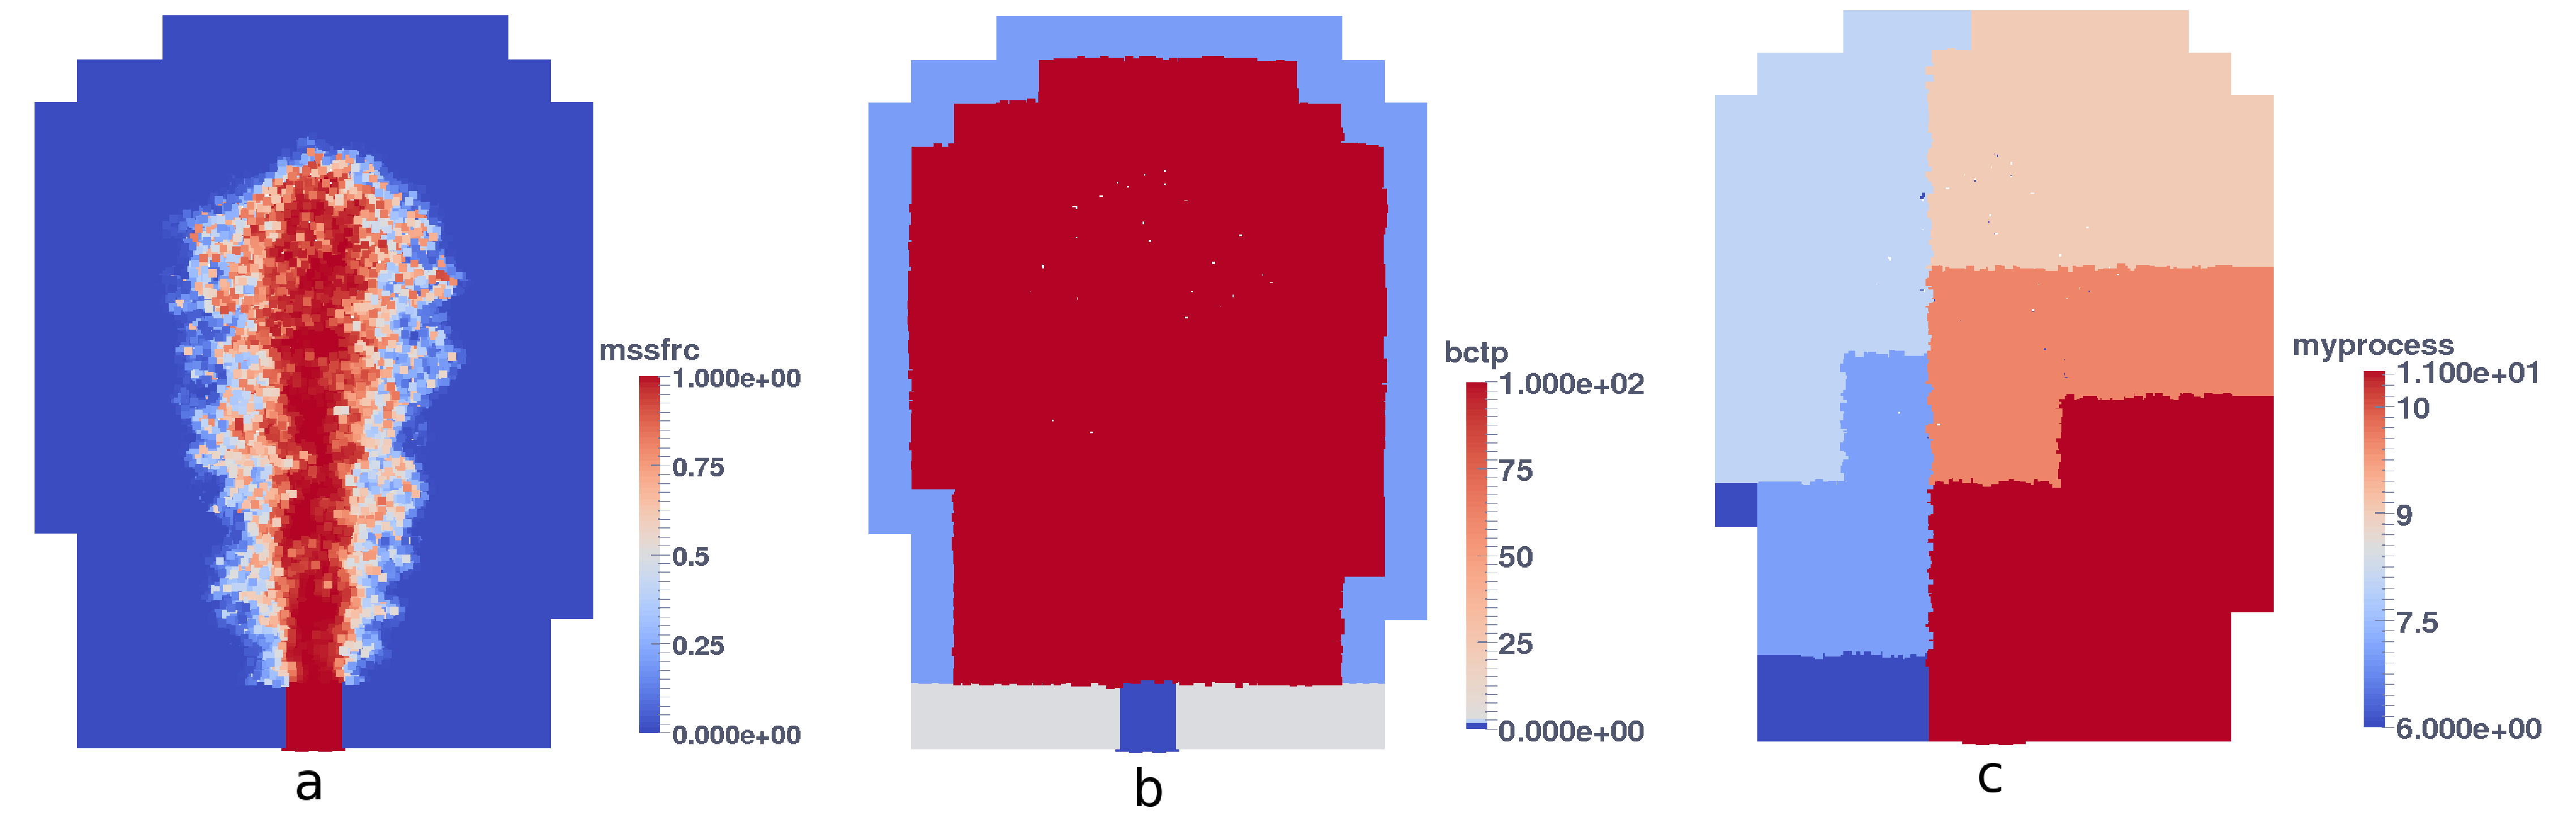
\includegraphics[width=18cm]{Chapter-3/Figures/t120_bc_proc}
\caption{A cross section view of the simulation domain in $y-z$ plane at 66 seconds. Subfigure $a$ shows the mass fraction. Subfigure $b$ shows all boundary conditions: the dark blue region are occupied by eruption ghost particles with "Ghost particle ID" of 0, the light blue area are occupied by pressure ghost particles with "Ghost particle ID" of 1, the gray area is filled with wall ghost particles with "Ghost particle ID" of 2, "Ghost particle ID" of all real particles are set to 100, they occupy the major portion of the domain in subfigure $b$. Subfigure $c$ shows the cross section view of domain decomposition based on SFC. The simulation is conducted on 12 processors, so there are 12 subdomains in total. The crosss section view shows a portion of them.}
\label{fig:bc_and_domain_decomp}
\end{figure}
\chapter{Godunov SPH and RCM SPH}

\section{Introduction}
Historically, SPH has difficulty in capturing discontinuities, such as shocks or contact discontinuities. Inviscid description of fluids becomes invalid at shock fronts, where specific entropy of the fluids increases through the conversion of mechanical energy into internal energy. Most SPH codes have included an artificial viscosity term explicitly, both for stabilizing the simulation and for handling shock discontinuities by dissipating local velocity differences and converting them into heat \citep{monaghan1983shock, monaghan1997sph, klapp2012strong}. Without knowing the minimum amount of dissipation for shock capturing, such methodology usually provides dissipation more than need and smears the discontinuity if the artificial viscosity coefficients are not tuned. The method of using constant artificial viscosity might also introduce spurious effects at region away from shocks, for instance, causing an unphysical damping of turbulent mixing (as shown, for example, by \citet{borgani2012hydrodynamic}) or spurious
shearing torques in rotating flows \citep{flebbe1994smoothed}. Selective application of artificial viscosity techniques, such as the time dependent viscosity \citep{morris1997switch, dolag2005turbulent} and shock-indicator-based viscosity \citep{cullen2010inviscid} have been tried for counteracting this. 
\citet{sigalotti2008adaptive} improved the standard SPH near sharp discontinuities adopting adaptive density kernel estimation (ADKE) techniques. However, the parameters for ADKE have to be tuned to the problem at hand \citep{puri2014comparison}. Hence it is hard to implement ADKE in real applications.

Besides adding dissipation explicitly, \citet{inutsuka2002reformulation} proposed an innovative approach to introduce dissipation implicitly by reformulating the SPH convolution integrals. Artificial viscosity is introduced implicitly by using iterative solution to a Riemann problem at an imaginary interface between an interacting particles pair. This method, named as Godunov SPH (GSPH), is attractive because it eliminates parameterization and hence user intervention associated with artificial viscosity coefficients. The GSPH method has been shown to be able to handle shock discontinuities \citep{inutsuka2002reformulation, cha2003implementations,iwasaki2011smoothed, puri2014approximate}, introduces less damping to turbulent mixing \citep{cha2010kelvin, borgani2012hydrodynamic} than standard SPH, and ameliorate pressure ``blips" (or ``wiggle" called by others) at the contact discontinuity \citep{borgani2012hydrodynamic}. However, the amount of dissipation introduced by GSPH is stll excessive than needs. When using a linear interpolation of the volume function, it has been shown \citep{borgani2012hydrodynamic} that the excess of diffusion, which manifests itself in the shock tube tests as a smooth transition at the rarefaction fan, is such to prevent the development of the Kelvin-Helmholtz (KH) instability.
%The development of KH instability is also significantly affected by number of neighbouring particles for cubic interpolation of the volume function.

The random choice method (RCM) was introduced by \citet{glimm1965solutions} for the construction of solutions of systems of nonlinear hyperbolic conservation laws. \citet{chorin1976random} developed the RCM as a practical computational method for solutions to one dimensional (1D) Euler equations of gas dynamics. Chorin's work was followed by numerous researchers, with applications and further improvements \citep{sod1977numerical,concus1979numerical,colella1982glimm, freistuhler1992numerical}. In essence, the solution is advanced in time by a sequence of operations that include solving of Riemann problems and a stochastic sampling of the solution. See \citep{toro2013riemann} for details. When applied to one dimensional time dependent Euler equations \citep{colella1982glimm}, diffusive errors from spatial averaging are completely eliminated and hence discontinuities, such as shocks or material interface, can be resolved as true discontinuities.
For unsteady flows in genuine two (or higher) space dimensions, however, such very desirable property of RCM do not seem to persist \citep{colella1982glimm}.
%This need to be proven ---> But at least, if the good property of preserving true discontinuity is still valid in 1D shock tube problem, it should be preserved in multiple-dimensional implementations. Because in current framework of RSPH, no matter what is the dimension of the problem, the techniques is only implemented in a one-dimensional scenario.

In this investigation, we introduce a new method, which will be referred to as RSPH in later paragraph, by integrating RCM method within framework of SPH. 
The new scheme inherits the attraction of classical RCM, introducing less but sufficient artificial viscosity and causing less smearing of discontinuities than other methods for 1D problems. Implementing of RCM within the framework of SPH only involves sampling of solutions of Riemann problem in 1D local coordinate system no matter what is the dimensionality of the problem. That is to say, no multi-dimensional coordinate is involved even for multi-dimensional problems. Thereby, the desirable property of RCM method in 1D should be retained in higher dimensional implementations within the framework of SPH. This hypothesis is confirmed by a three-dimensional (3D) free jet flow simulation. 

To summarize, RSPH has the following advantages over standard SPH:
\begin{itemize}
\item RSPH is able to capture discontinuities with less smearing.
\item The RSPH is able to adaptively adjust equivalent artificial viscosity coefficients, assigning larger artificial viscosity coefficients around the shock and small artificial viscosity coefficients otherwhere.
\item RSPH is able to alleviate pressure ``wiggle" at the contact discontinuity, a common issue in classical SPH.
\end{itemize}
Compared with GSPH, which is also based on solution of local Riemann problems, RSPH introduces less but sufficient dissipation than GSPH, especially in the region away from shocks. Such feature of RSPH is especially beneficial for simulating of scenarios involving turbulence mixing, for which excessive dissipation would suppress mixing. In addition, RSPH also shows faster convergence rate than GSPH.

The scheme of this chapter is follows. We start with a brief review of standard GSPH in the second section. The RSPH is then explained in details in the third section followed by the numerical tests section, where both one 1D and 3D inviscid Euler equations (see Eq. (\ref{eq:gov-cs-rho-er}) - (\ref{eq:gov-cs-e-er}) are solved by standard SPH, GSPH and RSPH. Limitations and potential applications of RSPH are discussed in last section. 

Investigation in this chapter implements RSPH scheme in solving inviscid compressile Euler equations as the application case.  
\begin{align}
\dfrac{\partial \rho}{\partial t} + \nabla \cdot \left(\rho \textbf{v} \right) = 0 \label{eq:gov-cs-rho-er} \\
\dfrac{\partial \rho \textbf{v}}{\partial t} + \nabla \cdot \left(\rho \textbf{v} \textbf{v} + p\textbf{I}\right) = 0 \label{eq:gov-cs-v-er} \\
\dfrac{\partial \rho E}{\partial t} + \nabla \cdot \left[\left(\rho E + p \right)\textbf{v}\right] = 0 \label{eq:gov-cs-e-er}
\end{align}
where $\rho$ is the density, $\textbf{v}$ is the velocity, $\textbf{I}$ is a unit tensor.
$E = e + K $ is the total energy which is a summation of kinetic energy $K$ and internal energy $e$.
The system of equations is closed by equation of state (EOS) for idea gas.
\begin{equation}
p = \left(\gamma - 1\right)\rho e \label{eq:EOS-er}
\end{equation}
with $\gamma=1.4$.

For any SPH scheme, governing equations in Lagrangian form are needed. By deducting kinetic energy from energy equation, subtracting mass conservation from momentum equation, combining transient term and advection term into material derivative term, the governing equations are converted into the Lagrange form. 
\begin{align}
\dfrac{D \rho}{D t} + \rho \nabla \cdot \textbf{v} = 0 \label{eq:gov-nc-rho-er}\\
\dfrac{D \textbf{v}}{D t} + \dfrac{\nabla P}{\rho} =0 \label{eq:gov-nc-v-er}\\
\dfrac{D e}{D t} + \dfrac{P \nabla \cdot \textbf{v}}{\rho} = 0 \label{eq:gov-nc-e-er}
\end{align}
%\cutet{puri2014comparison} propose an addition of an artificial heating term to the GSPH scheme to eliminate unphysical spikes in the thermal energy at the contact discontinuity.  --> It is worthwhile to check whether RSPH is able to avoid this phenomena without using his techniques.
%Another issue of RCM: the very desirable properties of RCM: no diffusive errors from spatial averaging do not seem to persist for flows in two space dimensions. For two dimensional steady supersonic flow, one of the space variables can be treated as a time-like one and RCM can be applied in a way similar to that for one-dimensional unsteady flow.
%--Then what about RSPH?

\section{GSPH method}
The RSPH method is based on standard SPH and GSPH. In addition, these three methods will be compared in the numerical tests section. Standard SPH has been discussed in detail in previous chaper. We present here a brief review on standard GSPH providing corresponding discretization of the compressible Euler equations.
 
In GSPH, the density field is updated in the same way as updating of density in SPH, according to Eq. (\ref{eq:ns-sph-d}). Updating of velocity and internal energy in GSPH is different from these in SPH. 
Derivation of discretized momentum and energy equation in first GSPH paper \citep{inutsuka2002reformulation} is based on the following discrete consistency identities: 
\begin{equation}
1=\sum_{b} \frac{m_{b}}{\rho(\textbf{x})}w(\textbf{x} - \textbf{x}_{b}, h)
\label{eq:GSPH-basic1}
\end{equation}
\begin{equation}
0=\sum_{b} m_{b} \nabla \frac{w(\textbf{x} - \textbf{x}_{b}, h)}{\rho(\textbf{x})}
\label{eq:GSPH-basic2}
\end{equation}
Lengthy algebraic manipulations \citep{inutsuka2002reformulation,iwasaki2011smoothed} lead to the discretized momentum and energy equations:
\begin{equation}
\ddot{\textbf{x}}_{a} = <\dfrac{d \textbf{v}_{a}}{dt}>= -\sum_{b} m_{b} p_{a b}^{\ast} \left[\frac{1}{\rho_{a}^2} \nabla w_{a b}(h_{a}) + \frac{1}{\rho_{b}^2} \nabla w_{a b}(h_{b}) \right]
\label{eq:gov-gsph-v-simple-form}
\end{equation}
\begin{equation}
<\dfrac{d e_{a}}{dt}>= - \sum_{b} m_{b} p_{a b}^{\ast} [\textbf{v}_{a b}^{\ast} - \dot{\textbf{x}}_{a}^{\ast}] \left[\frac{1}{\rho_{a}^2} \nabla w_{a b}(h_{a}) + \frac{1}{\rho_{b}^2} \nabla w_{a b}(h_{b}) \right]
\label{eq:gov-gsph-e-simple-form}
\end{equation}
where, $p_{a b}^{\ast}$ and $\textbf{v}_{a b}^{\ast}$ are obtained by solving a 1D Riemann problem constructed based on physical quantity of particle $a$ and particle $b$. The starred quantity are interpolated value of the solution to the Riemann problem at an imaginary interface. More discussion about the imaginary interface is in section \ref{sec:Picking-up-single-state}.
$\dot{\textbf{x}}_{a}^{\ast}$ is time centered velocity of particle $a$:
\begin{equation}
\dot{\textbf{x}}_{a}^{\ast} = <\textbf{v}_{a}> + \frac{\Delta t}{2} \ddot{\textbf{x}}_{a}
\end{equation}

The difference between this formulation and classical SPH formulations come from two sources: 
\begin{itemize}
\item the averaged (in certain sense) pressure and the effect of artificial viscosity is replaced by  $p^{\ast}$, obtained based on a local Riemann solver.
\item a time centered velocity is used, which satisfies the following identities approximately. 
\begin{equation}
\left( \textbf{v}_{a b}^{\ast} - \dot{\textbf{x}}_{a}^{\ast} \right) \approx -0.5 \textbf{v}_{a b}
\label{eq:SPH-GSPH-difference2}
\end{equation}
%Where $\textbf{v}_{a b}$ is defined as $\textbf{v}_a - \textbf{v}_b$.
\end{itemize}
Actually, Godunov's idea of using Riemann solver can be combined with other SPH discretization formulations as well \citep{cha2003implementations}. 

More technical details of GSPH are in section \ref{sec:RSPH-method}. The construction of Riemann problem, Riemann solvers and projection of picked solution of the Riemann problem back to global coordinate system are exactly the same in GSPH and RSPH. They are described in the next section. The way how to pick up the starred value from solution of the Riemann problem is the only difference between GSPH and RSPH. Detailed discussion is presented in section \ref{sec:Picking-up-single-state}. 

\section{RSPH method} \label{sec:RSPH-method}
RSPH shares many commonalities with SPH and GSPH, especially with GSPH. We adopt the same density updating formulation (see Eq. (\ref{eq:ns-sph-d})) for density updating in SPH, GSPH and RSPH. The same kernel function is used for all schemes. The equation for updating particle position (see Eq. (\ref{eq:SPH-update-pos})) is also the same for all schemes. Discretized governing equations for RSPH and GSPH are exactly the same as well. The common palces shared with classical SPH and GSPH are unnecessary to repeat in this section. We focus more on where RSPH is different from SPH and GSPH.

Both GSPH and RSPH borrow ideas of shock capturing techniques from mesh based method. There is a great deal of commonality between Godunov's method and RCM for mesh based method. Both of them utilize the solution of a local Riemann problem. The difference is that the RCM pick up a single state contained in the local solutions ``randomly" while Godunov's method take the integral average. 
Integrating of Godunov's idea within SPH framework (the GSPH method), however, does not take the integral average at all. Instead, a single state of the local Riemann solution at an imaginary interface is picked up and used to upgrade physical quantities through discretized governing equations (see Eq. (\ref{eq:gov-gsph-v-simple-form}) - Eq. (\ref{eq:gov-gsph-e-simple-form})). The RSPH method, proposed in this paper mimicking classical RCM, picks up the single state by stochastic sampling. So the difference between RSPH and GSPH is how to pick up the single state from solution of the Riemann problem.

Technical details for GSPH which are not coverred in section \ref{sec:GSPH-method} are also presented in this section.
The piecewise constant construction of Riemann problem, which is adopted in both RSPH and GSPH, is presented in section \ref{sec:RP-construction}. The way to pick up a single state from solutions to local Riemann problems are formulated in section \ref{sec:Picking-up-single-state}. It is a common practice in real implementations of Godunov's method to use approximate non-iterative Riemann solvers.
Two non-iterative Riemann solvers, Roe Riemann solver and HLLC (Harten, Lax and van Keer scheme with contact) Riemann solver \citep{toro1994restoration}, are adopted in GSPH. The HLLC type of Riemann solver \citep{toro1994restoration}, in which the contact wave is considered, is used in RSPH. Section \ref{sec:RP-solver} presents details on these Riemann solvers. 

The last second subsection is about generating of random numbers for RSPH. The RSPH algorithm is summarized in last subsection.

\subsection{Defining of local 1D Riemann problem} \label{sec:RP-construction}
A 1D Riemann problem need to be solved to obtain  $p_{a b}^{\ast}$ and $\textbf{v}_{a b}^{\ast}$ in both GSPH and RSPH. Hence, a 1D Riemann problem need to be constructed first. Constructing of 1D Riemann problem starts from establishing of a local coordinate system ($q$). The origin is selected at the middle-point of the line segment joining two particles with the unit vector along the line defined as: 
\begin{equation}
\hat{r}_{a b}= \frac{\textbf{x}_{a} - \textbf{x}_{ b}}{|\textbf{x}_{a} - \textbf{x}_{ b}|}
\end{equation}
Then vector variables, such as velocity, need to be projected onto the local coordinate system (Eq. (\ref{eq:RP-project-2-local-a}) and Eq. (\ref{eq:RP-project-2-local-b})). 
\begin{equation}
u_{a}= \textbf{v}_{a} \cdot \hat{r}_{a b}
\label{eq:RP-project-2-local-a}
\end{equation}
\begin{equation}
u_{b}= \textbf{v}_{b} \cdot \hat{r}_{a b}
\label{eq:RP-project-2-local-b}
\end{equation}
Scalar variables are simply assigned to corresponding points without projection.

The RSPH essentially takes the ``piece wise constant" manner for Riemann problem construction. No further step is required for construction after projection. Recall that in GSPH method, the construction of Riemann problem is divided into two sub-steps: projection and construction. 
Different from original Godunov's method, which assumes piecewise linear distribution of the data (or higher order method like MUSCL and PPM which use higher order polynomial approximation), RCM method assumes that the given data at the center of cell is constant throughout the respective cell. The same idea can be easily (and naturally) applied in RSPH as there is actually no cell in SPH method. Then the Riemann problem is defined directly based on data on particles. There is no need to calculate and project first order derivative of $\rho$, $u$ and $p$, which are needed for constructing of Riemann problem in a piece wise linear manner. The computation associated with calculation of gradient and projection of gradient is avoided when constructing 1D Riemann problem in such a ``piece wise constant" manner.
Per above description, the initial states at left and right sides are given as: 
\begin{eqnarray}
\rho_L = \rho_b 
\label{eq:Riemann-Prob-define-L-rho} \\
u_L = u_b 
\label{eq:Riemann-Prob-define-L-v} \\
p_L = p_b 
\label{eq:Riemann-Prob-define-L-p}
\end{eqnarray}
\begin{eqnarray}
\rho_R = \rho_a 
\label{eq:Riemann-Prob-define-R-rho} \\
u_R = u_a 
\label{eq:Riemann-Prob-define-R-v} \\
p_R = p_a 
\label{eq:Riemann-Prob-define-R-p}
\end{eqnarray}

\subsection{Picking up a single state} \label{sec:Picking-up-single-state}
Solving the 1D Riemann problem with initial right and left states (Eq. (\ref{eq:Riemann-Prob-define-L-rho}) - Eq. (\ref{eq:Riemann-Prob-define-R-p})) leads to a solution of the local system. Then pick up a single state and assign it to $p^{\ast}$ and $u^{\ast}$. The location where the single state is picked up is different for RSPH and GSPH. The starred values for RSPH takes the solution of the local Riemann problem at location $q_{ab}^{RSPH}$, which depends on a random number $\epsilon$. 
\begin{equation}
q_{ab}^{RSPH}=\epsilon \left( q_a - q_b \right) - \frac{| q_a + q_b|}{2}
\label{eq:sample-location-RSPH}
\end{equation}
At the nth time step, the same random number $\epsilon^n$ is used for picking up the single state from solutions of all local Riemann problems. For the next time step, the next pseudo random number $\epsilon^{n+1}$ will be used.
Recall that the starred value for GSPH is taken as solution of the local Riemann problem at a fixed location, denoted as $q_{ab}^{GSPH}$. In original GSPH, the imaginary interface is determined based on interpolation of the specific volume between two paired particles \citep{inutsuka2002reformulation}. We set the fixed location at the middle point \citep{cha2003implementations} for simplicity. 
\begin{equation}
q_{ab}^{GSPH}= 0
\label{eq:sample-location-GSPH}
\end{equation} 

Denote the solution of the local Riemann problem, either accurate or approximate, between a pair of particles ($a$ and $b$) to be $\textbf{W} (q), \  \forall q \in [q_a, q_b]$ (note, we use $\textbf{W}$ to represent the primitive variable vector $[\rho, u, p]^T$ and $\textbf{U}$ for conservative variable vector  $[\rho, \rho u, \rho E]^T$). The starred value for both GSPH and RSPH can be expressed in the same way:
\begin{equation}
p_{ab}^{\ast} = p \left(q_{ab}^{\ast} \right)
\label{eq:RSPH-Random-Pick-p}
\end{equation}
\begin{equation}
u_{ab}^{\ast} = u \left(q_{ab}^{\ast} \right)
\label{eq:RSPH-Random-Pick-u}
\end{equation}
where $q_{ab}^{\ast}=q_{ab}^{GSPH}$ for GSPH while $q_{ab}^{\ast}=q_{ab}^{RSPH}$ for RSPH. The random sample range for RSPH and imaginary interface for GSPH is shown in Fig. \ref{fig:pick-up-state-GSPH-RSPH}.
\begin{figure}[H]
    \center
	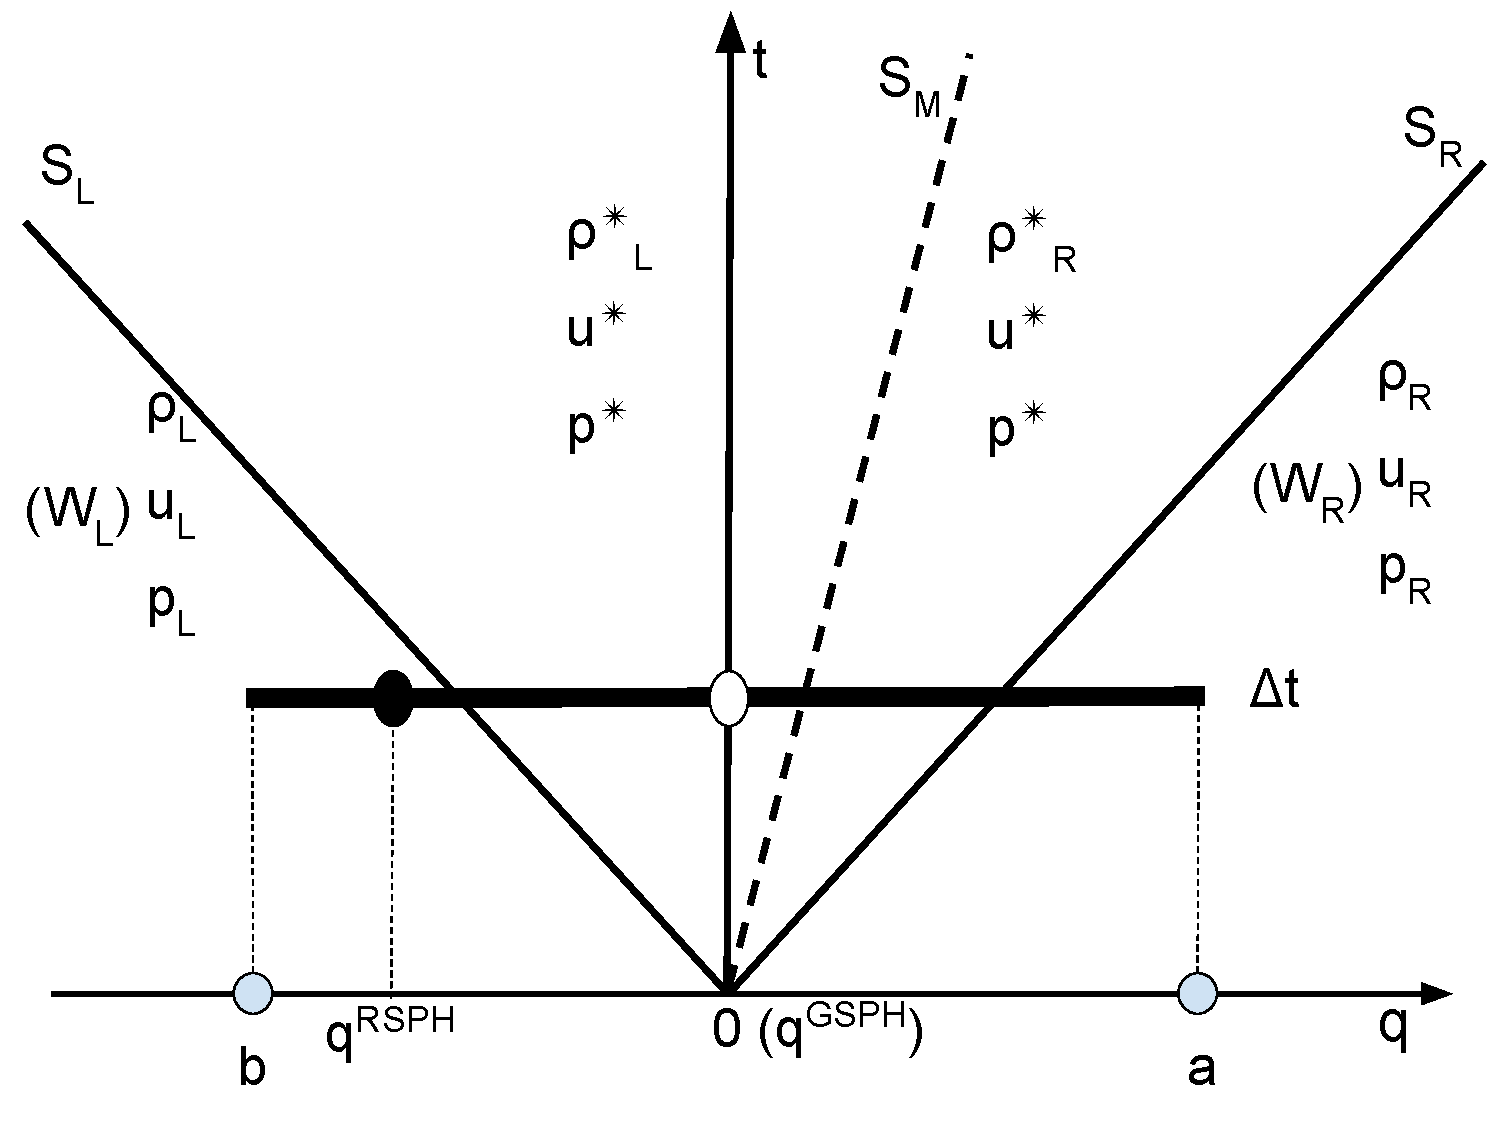
\includegraphics[width=0.5 \textwidth]{Chapter-4/Figures/RSPH-GSPH}
    \caption{Evaluating of the starred values in RSPH and GSPH for paired particles $a$ and $b$. The local Riemann problem is defined by state of particles $a$ and $b$ at $t=0$ according to Eq. (\ref{eq:Riemann-Prob-define-L-rho}) - Eq. (\ref{eq:Riemann-Prob-define-R-p})). The horizontal bold solid line indicate the sample range in the solution of the Riemann problem defined between particle $a$ and particle $b$ at given time $t=\Delta t$. The dark ellipse is an example sample point of RSPH with the random number $\epsilon < \frac{1}{2}$. Depending on the random number $\epsilon$, the sample points can be anywhere on the horizontal bold solid line. The white ellipse is the imaginary interface for GSPH, which is fixed. The sampled state is assigned to starred velocity and pressure in Eq. (\ref{eq:gov-gsph-v-simple-form}) and Eq. (\ref{eq:gov-gsph-e-simple-form}) for both GSPH and RSPH.}
    \label{fig:pick-up-state-GSPH-RSPH}
\end{figure}

A short comments regarding the difference between application of RCM method in SPH and its application in finite volume method. In finite volume method, for 1D case, two Riemann Problems are definied on interfaces of both sides. the superposition of solutions of these two Riemann problems is taken as local solution within the cell and the sampled single state is assigned to the cell center. In RSPH, only one Riemann problem is defined between two particles and the sampled single state (the $p^{\ast}$ and $u^{\ast}$) is used in momentum and energy updating.

$u^{\ast}$ is velocity in a 1D local space and needs to be projected back to global space to obtain $\textbf{v}^{\ast}$ in cases of multi-dimensional implementations. One of such back-project approximations is:
\begin{equation}
\textbf{v}^{\ast}_{a b}=u^{\ast}_{a b} \hat{\textbf{r}}_{a b} + \left [\frac{\textbf{v}_{a} + \textbf{v}_{b}}{2} - \frac{u_L + u_R}{2} \hat{\textbf{r}}_{a b}\right]
\label{eq:RP-project-to-3d-arithmetic}
\end{equation}
In Eq. (\ref{eq:RP-project-to-3d-arithmetic}), the arithmetic average of shear velocity is taken as the shear velocity at the sample points. Alternative approximation might be distance weighted average or Roe average (weighted by square root of density). If $q_{a b}^{\ast}$ is assumed to be zero, then distance weighted average will degenerate to the arithmetic average.
Such back projection is required for both GSPH and RSPH.

We have to mention that it is strange in GSPH to assume an imaginary interface, which never need in RSPH. And that's one of the reasons why we like RSPH more.

\subsection{Non-iterative Riemann solvers} \label{sec:RP-solver}
The starred variable $p^{\ast}$ and $u^{\ast}$ represent the interpolated pressure and velocity at certain point (an imaginary interface in GSPH or a randomly sampled poit in RSPH) along the line joining the pairs of two particles. They do not have to be obtained by solving a Riemann problem. However, $p^{\ast}$ and $u^{\ast}$ obtained by solving a Riemann problem provides necessary and sufficient dissipation needed to capture discontinuities and stabilize the scheme.

The exact Riemann solver, even though more accurate and robust, requires an iterative root finding, and hence is computational inefficient. For governing equations other than well studied ones, such as Euler equations, there is no iterative Riemann solver available. Non-iterative approximate Riemann solvers can relieve these drawbacks of exact Riemann solvers. Among the available Riemann solvers \citep{rider1994review, luo2004computation, puri2014approximate}, we adopted the HLLC approximate Riemann solver.
The HLLC solver is a 3-wave approximate Riemann solver proposed by \citet{toro1994restoration}. In this work, we adopt the formulation of the HLLC solver proposed by \citet{luo2004computation} for multi-material, underwater explosions in their ALE scheme. This Riemann solver has the properties of being positivity preserving for scalar quantities, entropy satisfying and to exact preserve isolated contacts.

Equation (\ref{eq:RP_solver_HLLC_u}) and (\ref{eq:RP_solver_HLLC_pu}) are the approximate solution to the local Riemann problem, written in term of $p$ and $pu$ as functions of local coordinate $q$.
\begin{equation}
p \left( q \right) =  \begin{cases} 
      p_L & if \  S_L \Delta t> q \\
      \frac{S_M}{S_L - S_M}\left [ (S_L - \hat{u}_L) M_L + (\hat{p}- p_L) \right] + \hat{p} & if \  S_L \Delta t \leq q \leq S_M \Delta t \\
      \frac{S_M}{S_R - S_M}\left [ (S_R - \hat{u}_R) M_R + (\hat{p}- p_R) \right] + \hat{p} & if \  S_M \Delta t \leq q \leq S_R \Delta t \\
      p_R & if \  S_R \Delta t < q
\end{cases}
\label{eq:RP_solver_HLLC_u}
\end{equation}
\begin{equation}
(pu) \left( q \right)  =  \begin{cases} 
      p_L u_L& if \  S_L \Delta t > q \\
      \frac{S_M}{S_L - S_M}\left [ (S_L - \hat{u}_L) E_L + (\hat{p} S_M - p_L \hat{u}_L) \right] + (S_M - \hat{u}_{LR}) \hat{p} & if \  S_L \Delta t \leq q \leq S_M \Delta t \\
      \frac{S_M}{S_R - S_M}\left [ (S_R - \hat{u}_R) E_R + (\hat{p} S_M- p_R \hat{u}_R) \right] + (S_M + \hat{u}_{LR}) \hat{p} & if \ S_M \Delta t \leq q \leq S_R \Delta t\\
      p_R u_R & if \  S_R \Delta t < q
\end{cases}
\label{eq:RP_solver_HLLC_pu}
\end{equation}
where $\hat{u}_{LR}$ is the interface velocity and is taken as the Roe-averaged velocity on either side of the interface \citep{cheng2007high}. The quantities of $\hat{u}_R$ and $\hat{u}_L$ are velocities relative to the interface velocity.
\begin{equation}
\hat{p}= \rho_L (\hat{u}_L - S_L) (\hat{u}_L - S_M) + p_L
\end{equation}
Formulation to approximate the signal speeds $S_M$, $S_L$ and $S_R$ is given by Eq. (\ref{eq:RP-solver-HLLC-SM}) to (\ref{eq:RP-solver-HLLC-SR}).
\begin{eqnarray}
S_M= \frac{\rho_R \hat{u}_R (S_R - \hat{u}_R) - \rho_L \hat{u}_L (S_L - \hat{u}_L) + p_L - p_R}{\rho_R (S_R - \hat{u}_R) - \rho_L (S_L - \hat{u}_L)} \label{eq:RP-solver-HLLC-SM} \\
S_L = min (\hat{u}_L - c_L, -c_{LR}) \label{eq:RP-solver-HLLC-SL} \\
S_R = max (\hat{u}_R - c_R, c_{LR}) \label{eq:RP-solver-HLLC-SR}
\end{eqnarray}
where $c_{LR}$ is the relevant Roe averaged sound speed \citep{cheng2007high}. 

Besides HLLC, another 2-wave approximate Riemann solver, the Roe Riemann solver \citep{roe1981approximate}, is also adopted in GSPH.
Roe Riemann solver is proposed by \citet{roe1981approximate} to linearize the Euler equations and approxiamte the solution of non-linear system by a system of linear equations. The characteristic decomposition of the linearized Lagrangian flux and Jacobia matrices are used to write the flux. \citet{rider1994review} proposed an algebraic averaging of the Lagrangian variables, which is adopted in this work. Since Roe solver is only used in GSPH. We directly provide here the resulting starred values of the pressure and velocity \citep{puri2014approximate}: 
\begin{eqnarray}
u^{\ast} = \frac{1}{2} \left[ u_L + u_R - \frac{1}{C_{LR}} (p_R - p_L) \right] \label{eq:RP-solver-ROE-u} \\
p^{\ast} = \frac{1}{2}\left[ p_L + p_R - C_{LR} (u_R - u_L) \right] \label{eq:RP-solver-ROE-p}
\end{eqnarray}
Where $C_{LR}$ is the averaged Lagarangian sound speed at the interface.
\begin{equation}
C_{LR} = \sqrt{\gamma p_{LR} \rho_{LR}}
\end{equation}

\subsection{Binary Van Der Corput pseudo-random numbers} \label{sec:Van-Der-Corput-random-num}
The random number $\epsilon$ is used to determine the sample location $q_{ab}^{RSPH}$. The quantity of the computed RCM solution depends crucially on the random number $\{\epsilon ^n\}$. We adopt the Van Der Corupt pseudo-random number sequence \citep{hammersley2013monte} in this investigation following \citet{colella1982glimm}.

A general Van Der Corupt pseudo-random number sequence depends on two parameters $x_1$ and $x_2$ with $x_1 > x_2 > 0$, both are integer and relatively prime. The sequence is formally defined as \citep{hammersley2013monte}:
\begin{equation}
\epsilon ^n = \sum_{i=0}^{s} H_i x_1^{-(i+1)}
\label{eq:Van-Der-Corput-pseudo-random-num}
\end{equation}
where
\begin{equation}
H_i = x_2 a_i(mod \ x_1)
\label{eq:Van-Der-Corput-pseudo-random-num-Hi}
\end{equation} 
\begin{equation}
n = \sum_{i=0}^{s} a_i x_1^i
\label{eq:Van-Der-Corput-pseudo-random-num-n}
\end{equation} 
Equation (\ref{eq:Van-Der-Corput-pseudo-random-num-n}) gives the binary expansion of n when we take $x_1$ as $2$. For example,
\begin{equation}
5=1 \times 2^0 + 0 \times 2^1 + 1 \times 2^2
\end{equation}
with $m=2$. 

The next stage is to find the coefficient $H_i$ according to Eq. (\ref{eq:Van-Der-Corput-pseudo-random-num-Hi}). If we take $x_2 = 1$, for which case, $H_i = a_i, \ \forall i$. Having $H_i$, $x_1$ and $s$ ready, the random number $\epsilon ^n $ can be easily obtained according to Eq. (\ref{eq:Van-Der-Corput-pseudo-random-num}).
We take $x_1=2$  and $x_2 =1$ in this paper. Other combinations of $x_1$ and $x_2$ were also discussed by \citet{toro2013riemann}. A desirable statistical property of the sequence $\{\epsilon ^n\}$ is that $\{\epsilon ^n\}$ be uniformly distributed over $[0,1]$.
 
The arithmetic mean and the standard deviation of 200 binary Van Der Corput pseudo-random numbers are $0.49459$ and $0.28885$. The chi-square statistic (see \citet{toro2013riemann} for its calculation) $\chi_{sq}$ is $1.0000$. 
The binary Van Der Corput pseudo-random numbers are generated offline to save computational time.

%\subsection{Convergence}

\subsection{RSPH algorithm (the PESB algorithm)}
The Godunov's method is summarized as a REA (reconstruct, evolve, average) algorithm. Here we summarize the RSPH algorithm as a PESB (project, evolve, sample, back-project) algorithm. 
\begin{itemize}
\item For any two pair of particles, establish a local coordinate system whose axis joints these two particles then project the primitive variables vector onto the local coordinate system.
\item Evolve the hyperbolic equation exactly or approximately with Riemann problem defined by the projected data to obtain a solution between these two particles.
\item Sample these solutions between the particles pair to pick up a state and assign it to $p^{\ast}$ and $u^{\ast}$
\item Project $p^{\ast}$ and $u^{\ast}$ from local coordinate system back to the global coordinate system obtaining $p^{\ast}$ and $\textbf{v}^{\ast}$.
\end{itemize}
PESB algorithm is integrated into framework of SPH discretization to update physical quantities in time. PESB also fit well with GSPH, for which, the sample step is not stochastic randomly sample.

\section{Numerical tests}
We carry out several numerical tests using SPH, RSPH and GSPH in this section.
1D shock tube tests are conducted to compare standard SPH, GSPH and RSPH. Comprehensive shock tube tests are also conducted to check the capacity of RSPH for different situations. In addition, order of accuracy is investigated based on 1D shock tube problem. 
In the last subsection, a 3D free jet flow is simulated with SPH, GSPH and RSPH to check equivalent overall dissipation introduced by each method.

Input parameters for 1D tests can be found in Table \ref{tab:1D-shock-input_parameters}. 
\begin{table}[htp]
\centering
      \caption{Overview of 1D shock tube tests}		
	  \begin{tabular}{lrrrrrrrrrr}
	    \hline
	          & $\rho_L$ & $p_L$ &$v_L$ & $\rho_R$ & $p_R$ &$v_R$ & $m$ & $[x_L, x_R]$ & $t_f$\\
	    \hline
	    Test 1 & $1.0$ & $1.0$ &$0$ & $0.25$ & $0.1795$ &$0$ & $0.003$  & $[-0.4, 0.4]$ & $0.17$\\
	    	Test 2 & $1.0$ & $1.0$ &$0$ & $0.5$ & $0.2$ &$0$ & $0.003$  & $[-0.4, 0.4]$ & $0.2$\\
	    	Test 3 & $2.0$ & $1.95$ &$1.0$ & $1.0$ & $1.95$ &$-1.0$  & $0.006$  & $[-0.4, 0.4]$ & $0.13$\\
	    Test 4 & $1.0$ & $2.4$ &$8.0$ & $0.5$ & $0.4$ &$-0.25$ & $0.003$  & $[-0.4, 0.4]$ & $0.05$\\
	    	Test 5 & $1.0$ & $-2.0$ &$0.4$ & $1.0$ & $0.4$ &$2.0$ & $0.003$  & $[-0.4, 0.4]$ & $0.18$\\
	    	Test 6 & $1.0$ & $0$ &$1000$ & $1.0$ & $0$ &$0.01$ & $0.003$  & $[-0.5, 0.5]$  & $0.01$\\
	    \hline
	  \end{tabular}
	  \label{tab:1D-shock-input_parameters}
\end{table}
where, subscript $L$ refers left side and $R$ for right side. $m$ is particle mass, initial interval between adjacent particles are adjusted to guarantee equal particle mass. $t_f$ is the time to terminate simulation and plotting the results. Equal particle mass is assigned to all particles. The $x$ axis in all plots is normalized by time, that is $x/t_f$, in plots for shock tube tests results.

Test 1 consists of a left rarefaction, a right travelling contact and a right shock. Density increases at down wind of contact wave.
Test 2 also consists of a left rarefaction, a right travelling contact and a right shock. Density decreases at down wind of contact wave.
Test 3 includes double expansion waves. The initial density are different at right and left hand side.
Test 4 is a double shock tests with different initial density on the right side and left side.
Test 5 and Test 6 are two extreme cases. Test 5 is a cavity flow while test 6 is a strong blast flow.

\subsection{Comparison of RSPH with standard SPH and GSPH}
\begin{figure}[htp]
    \centering
    \begin{minipage}{.495\textwidth}
        \centering
        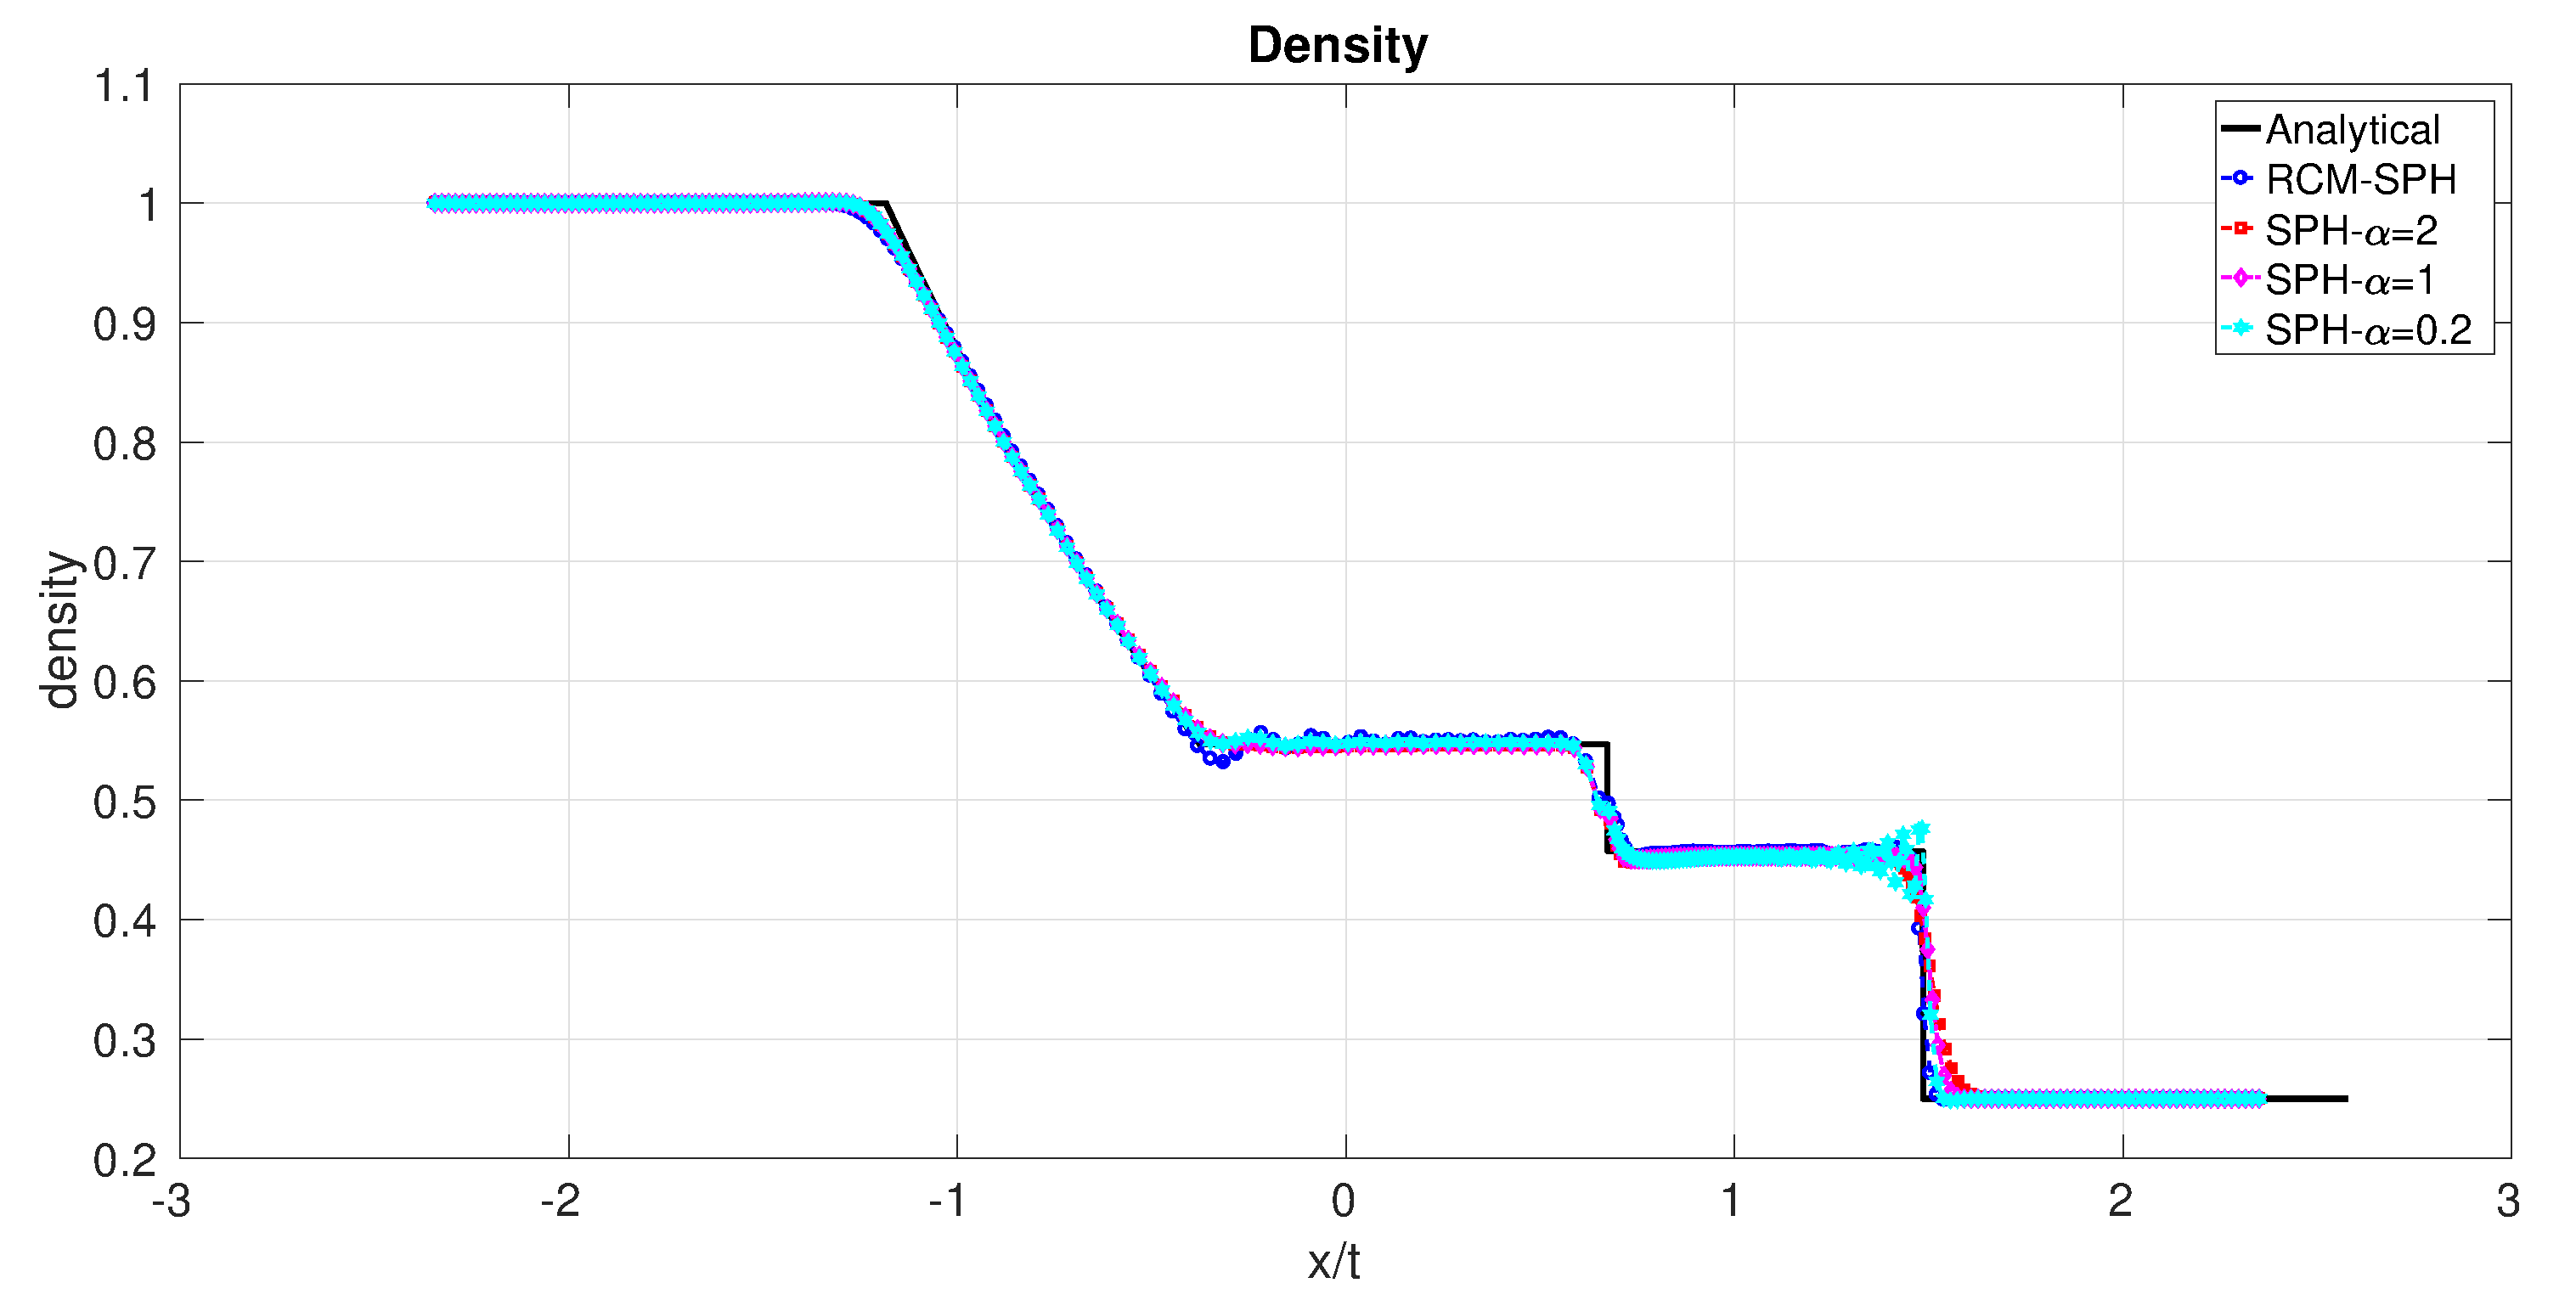
\includegraphics[width=0.99 \textwidth]{Chapter-4/Figures/Sod/RCM-Sod-SPH-alf-rho}
    \end{minipage}%
    \begin{minipage}{.495 \textwidth}
        \centering
        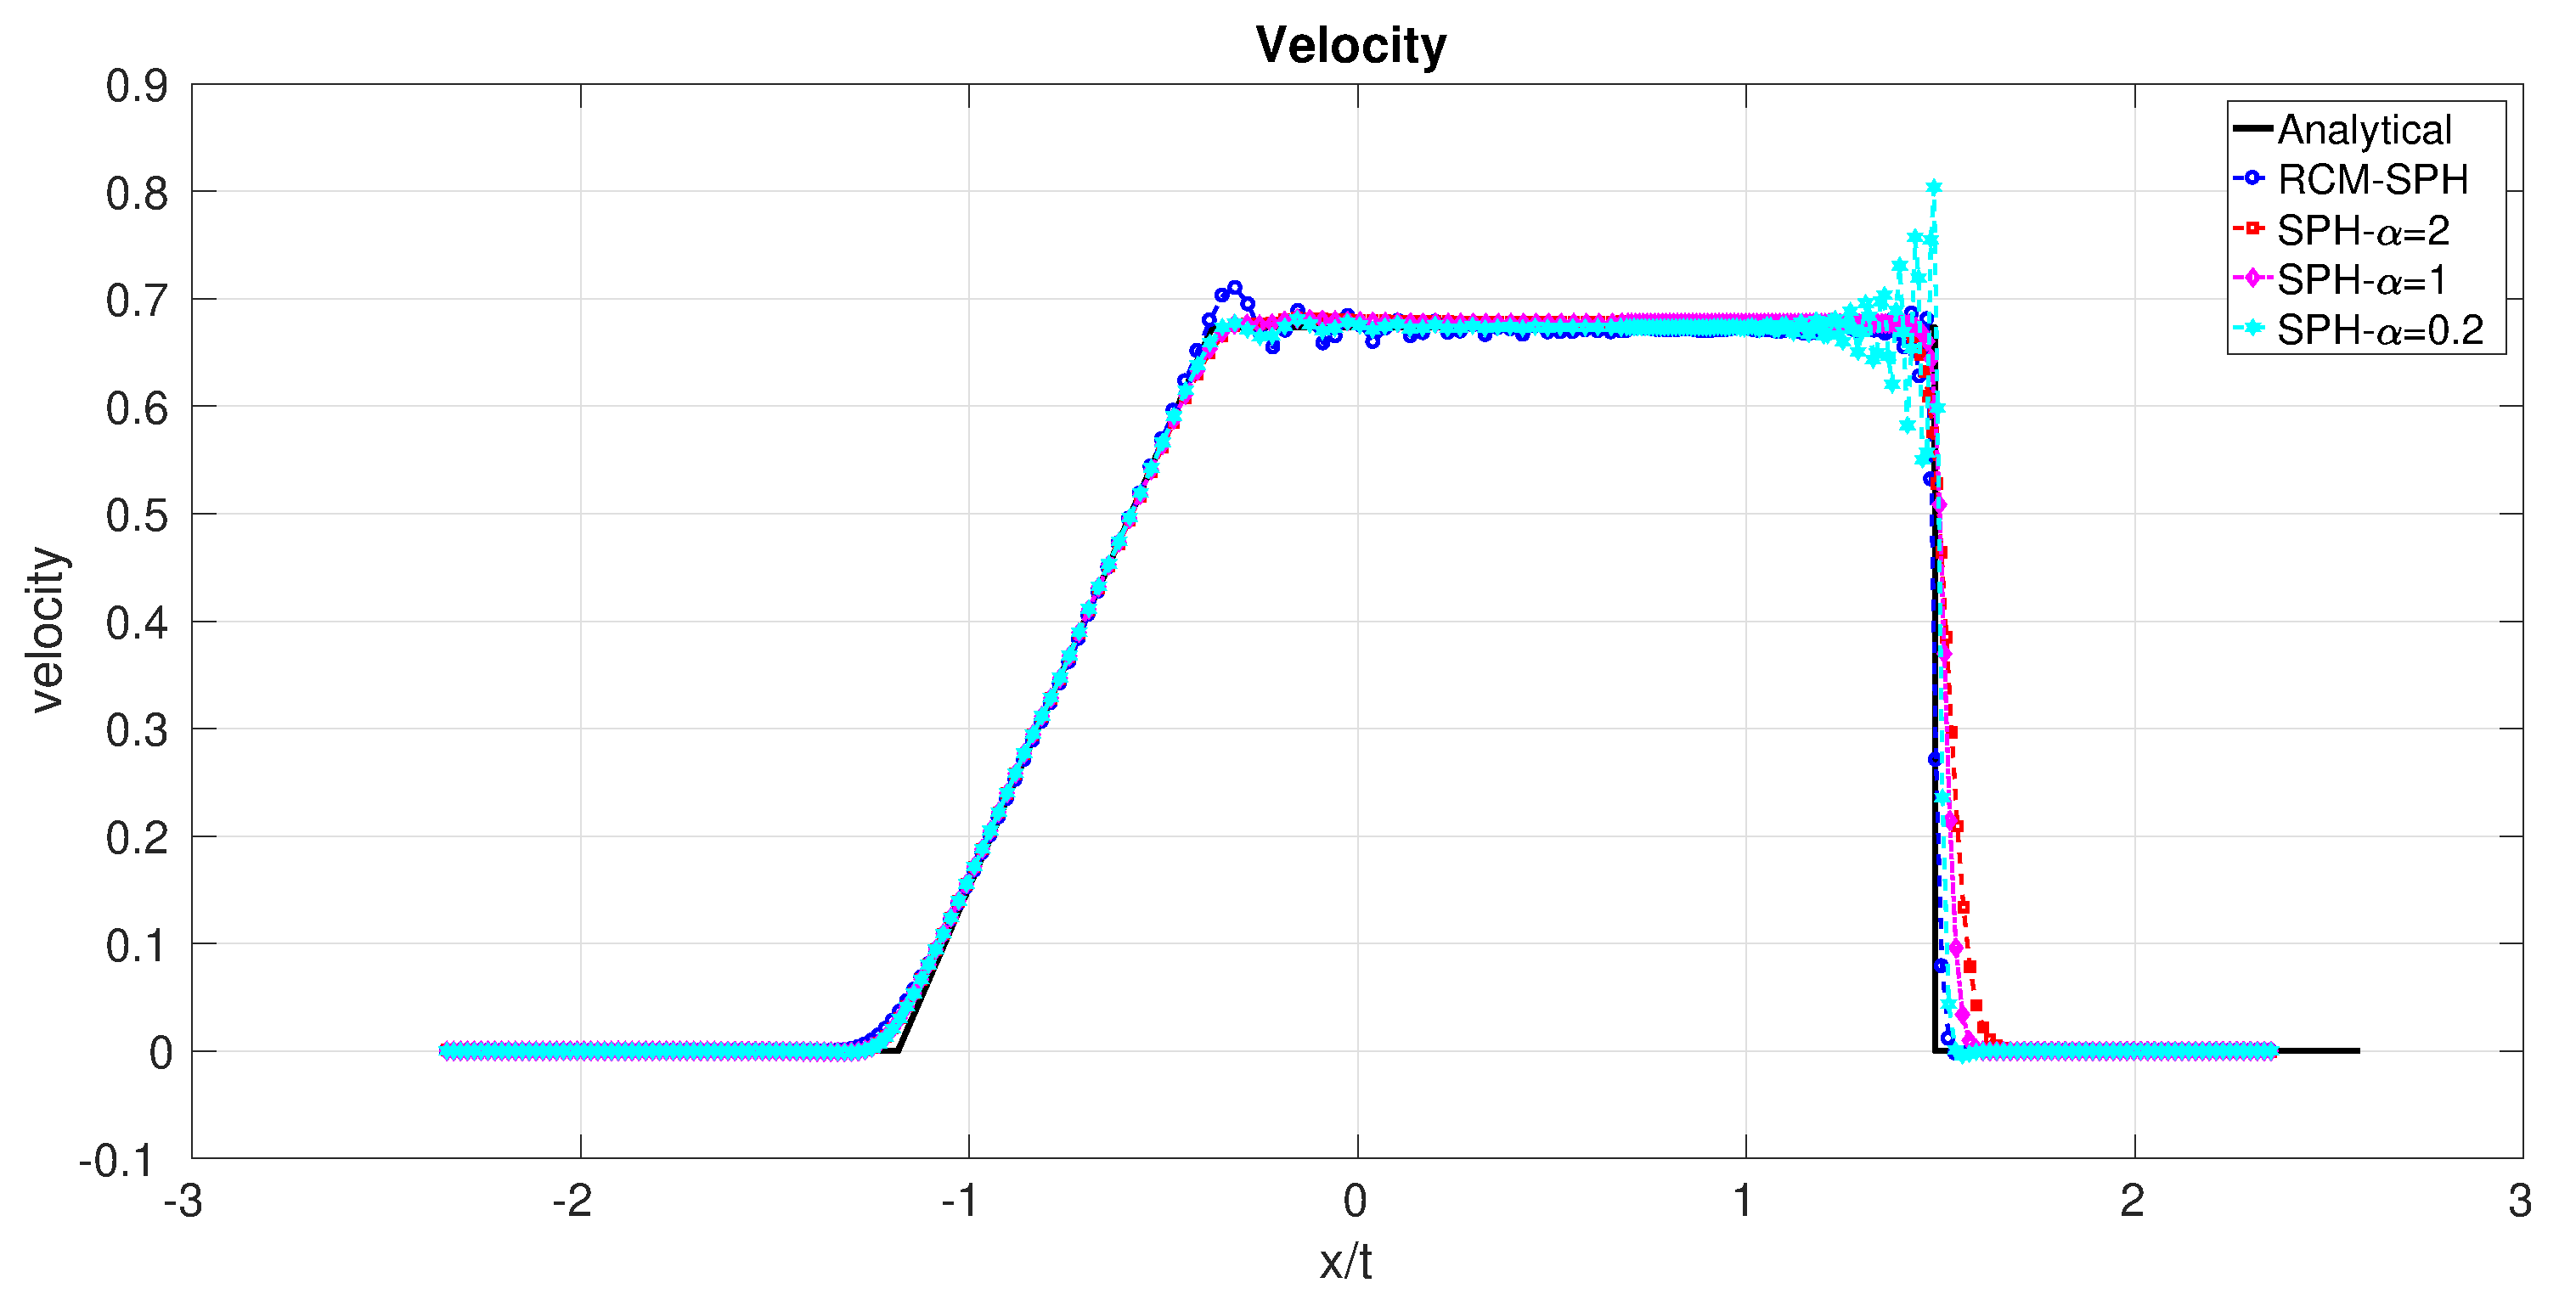
\includegraphics[width=0.99 \textwidth]{Chapter-4/Figures/Sod/RCM-Sod-SPH-alf-v}
    \end{minipage}%
    \\
    \begin{minipage}{.495\textwidth}
        \centering
        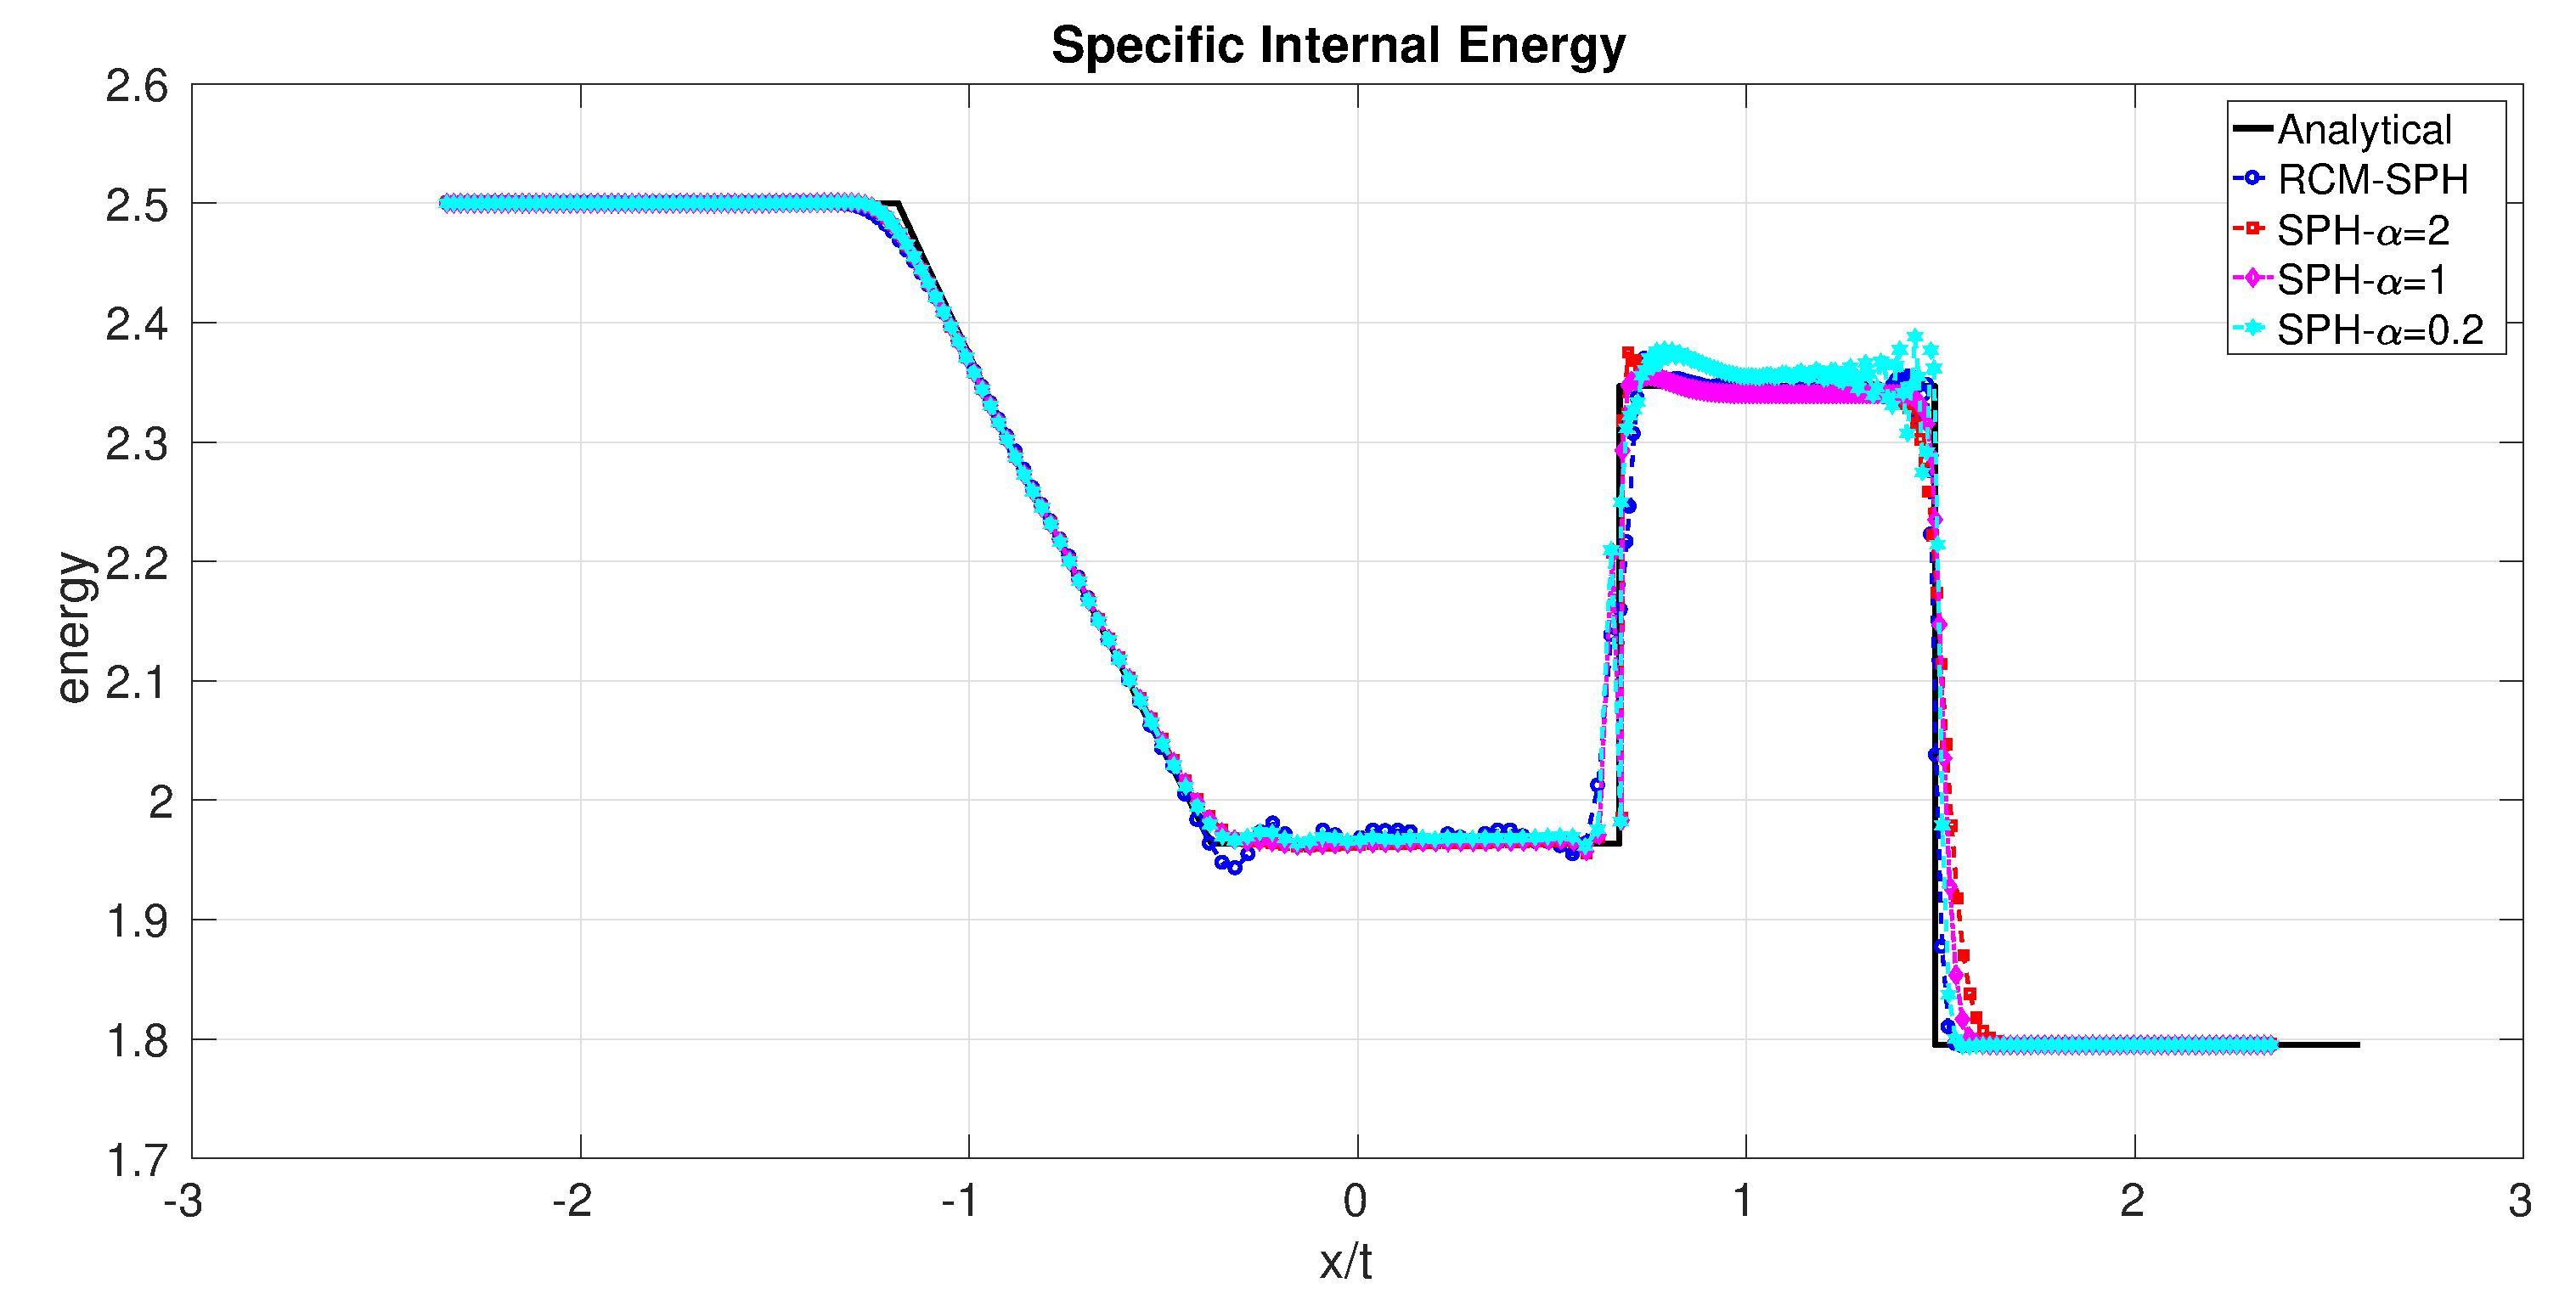
\includegraphics[width=0.99 \textwidth]{Chapter-4/Figures/Sod/RCM-Sod-SPH-alf-e}
    \end{minipage}%
    \begin{minipage}{.495 \textwidth}
        \centering
        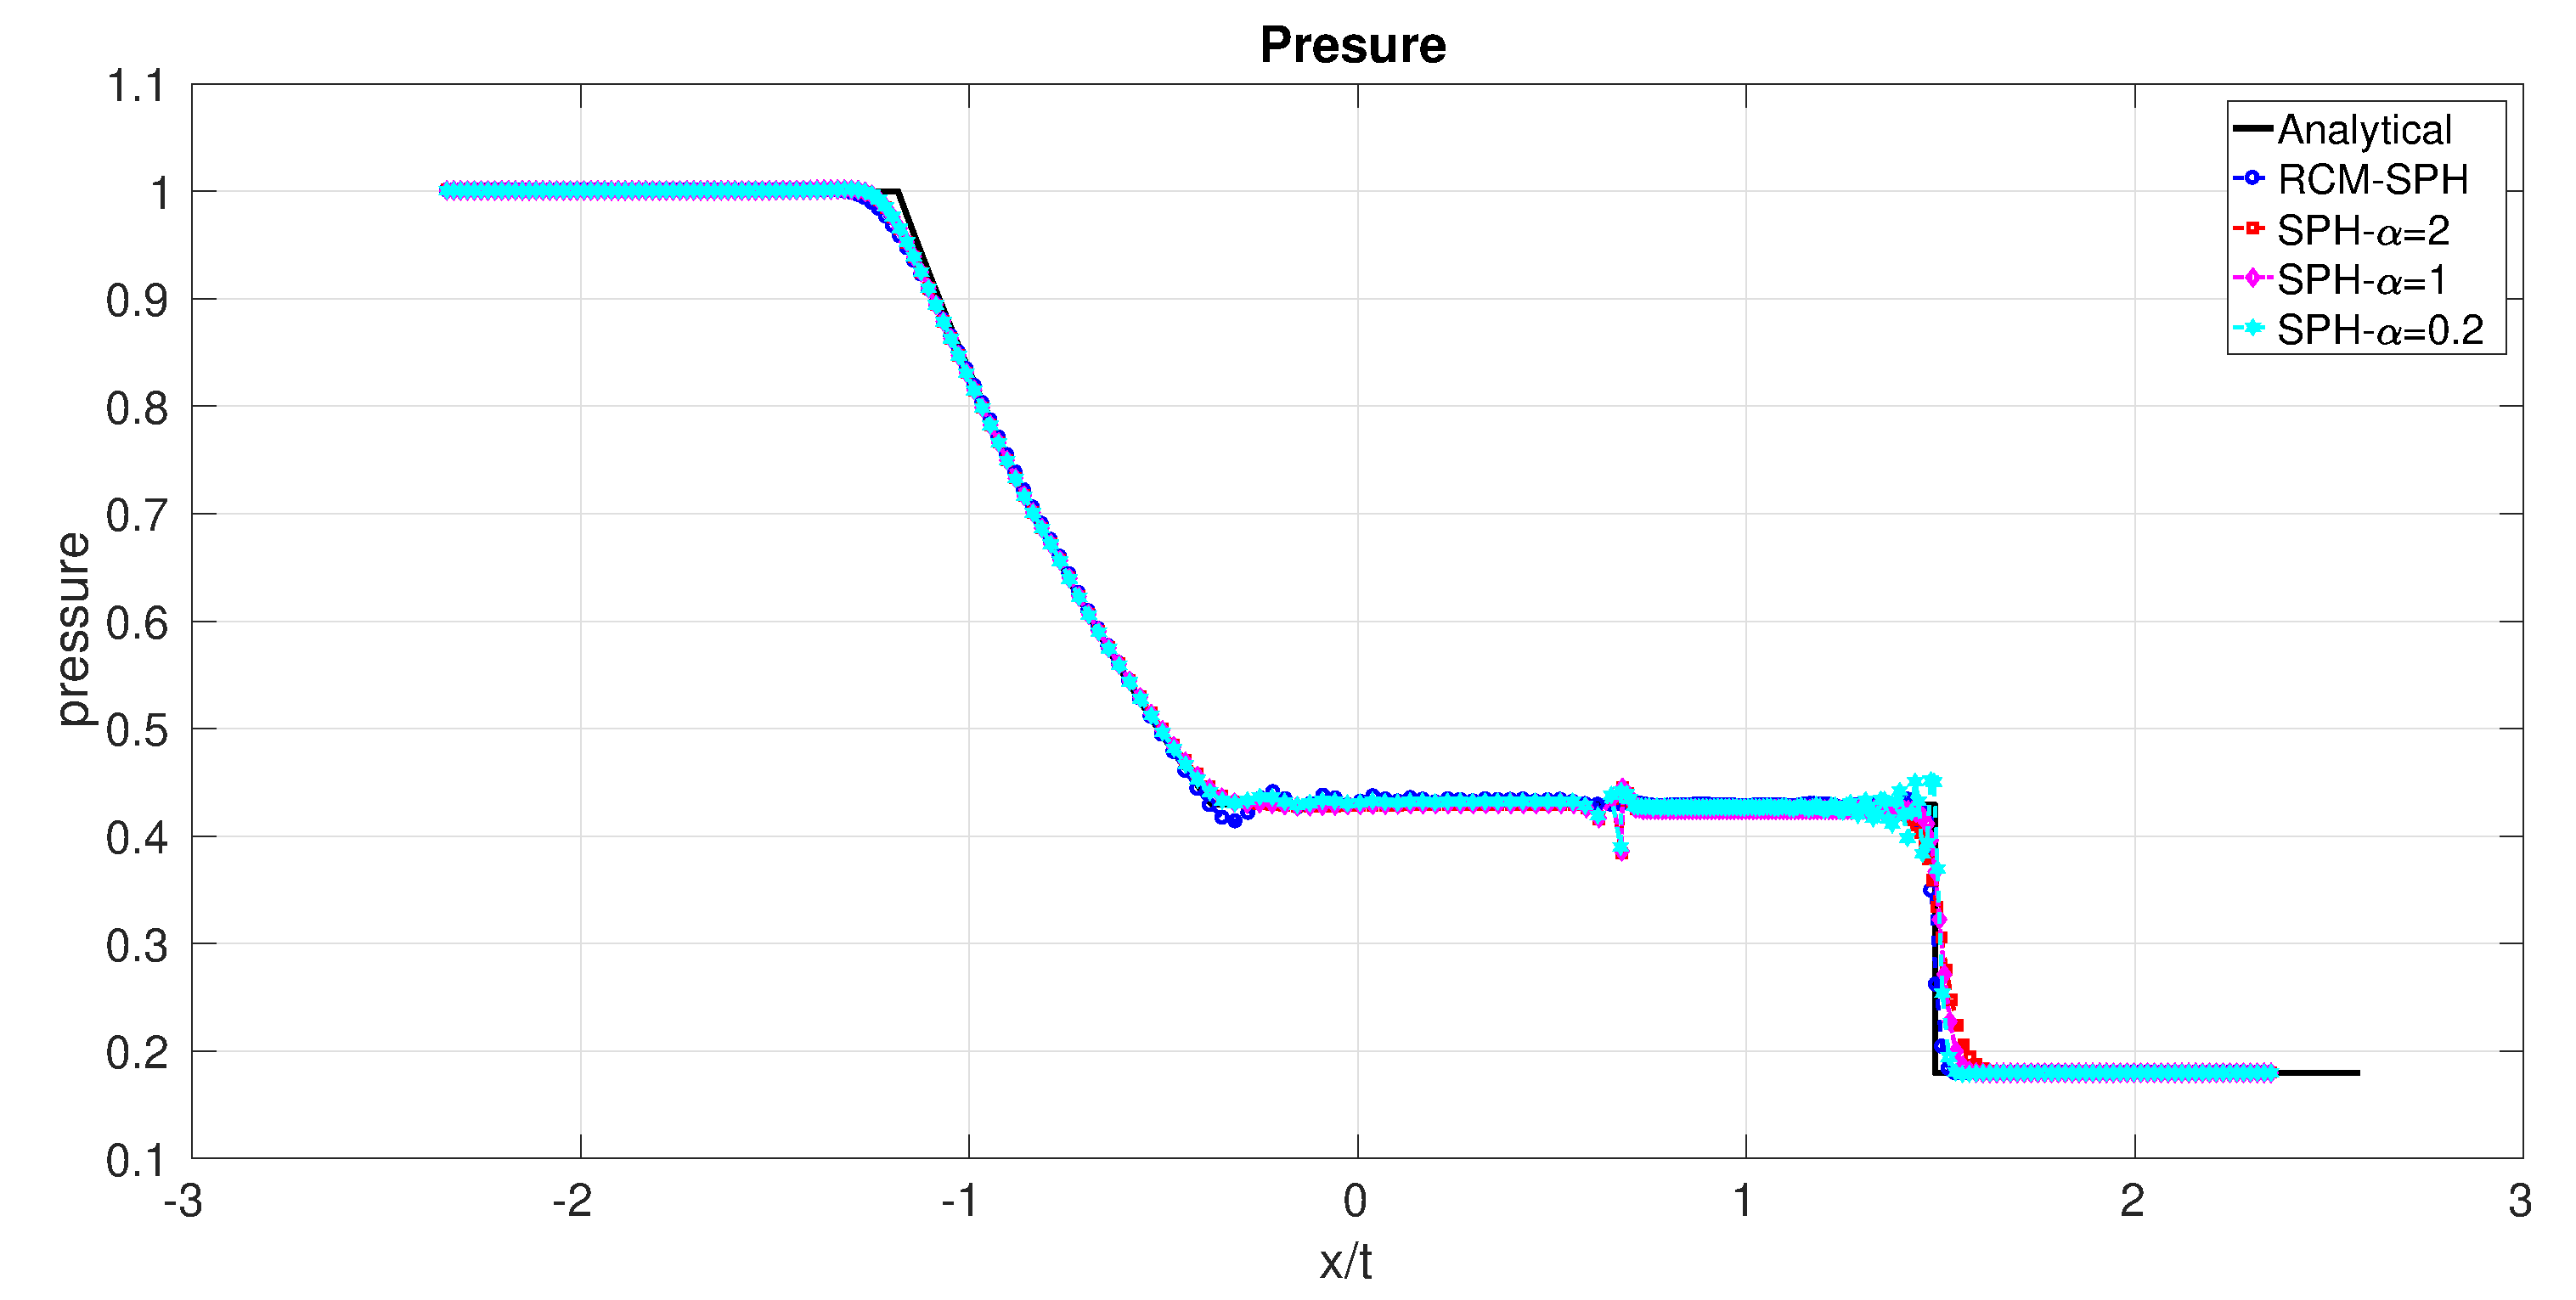
\includegraphics[width=0.99 \textwidth]{Chapter-4/Figures/Sod/RCM-Sod-SPH-alf-p}
    \end{minipage}% 
    \\
    \begin{minipage}{.495\textwidth}
        \centering
        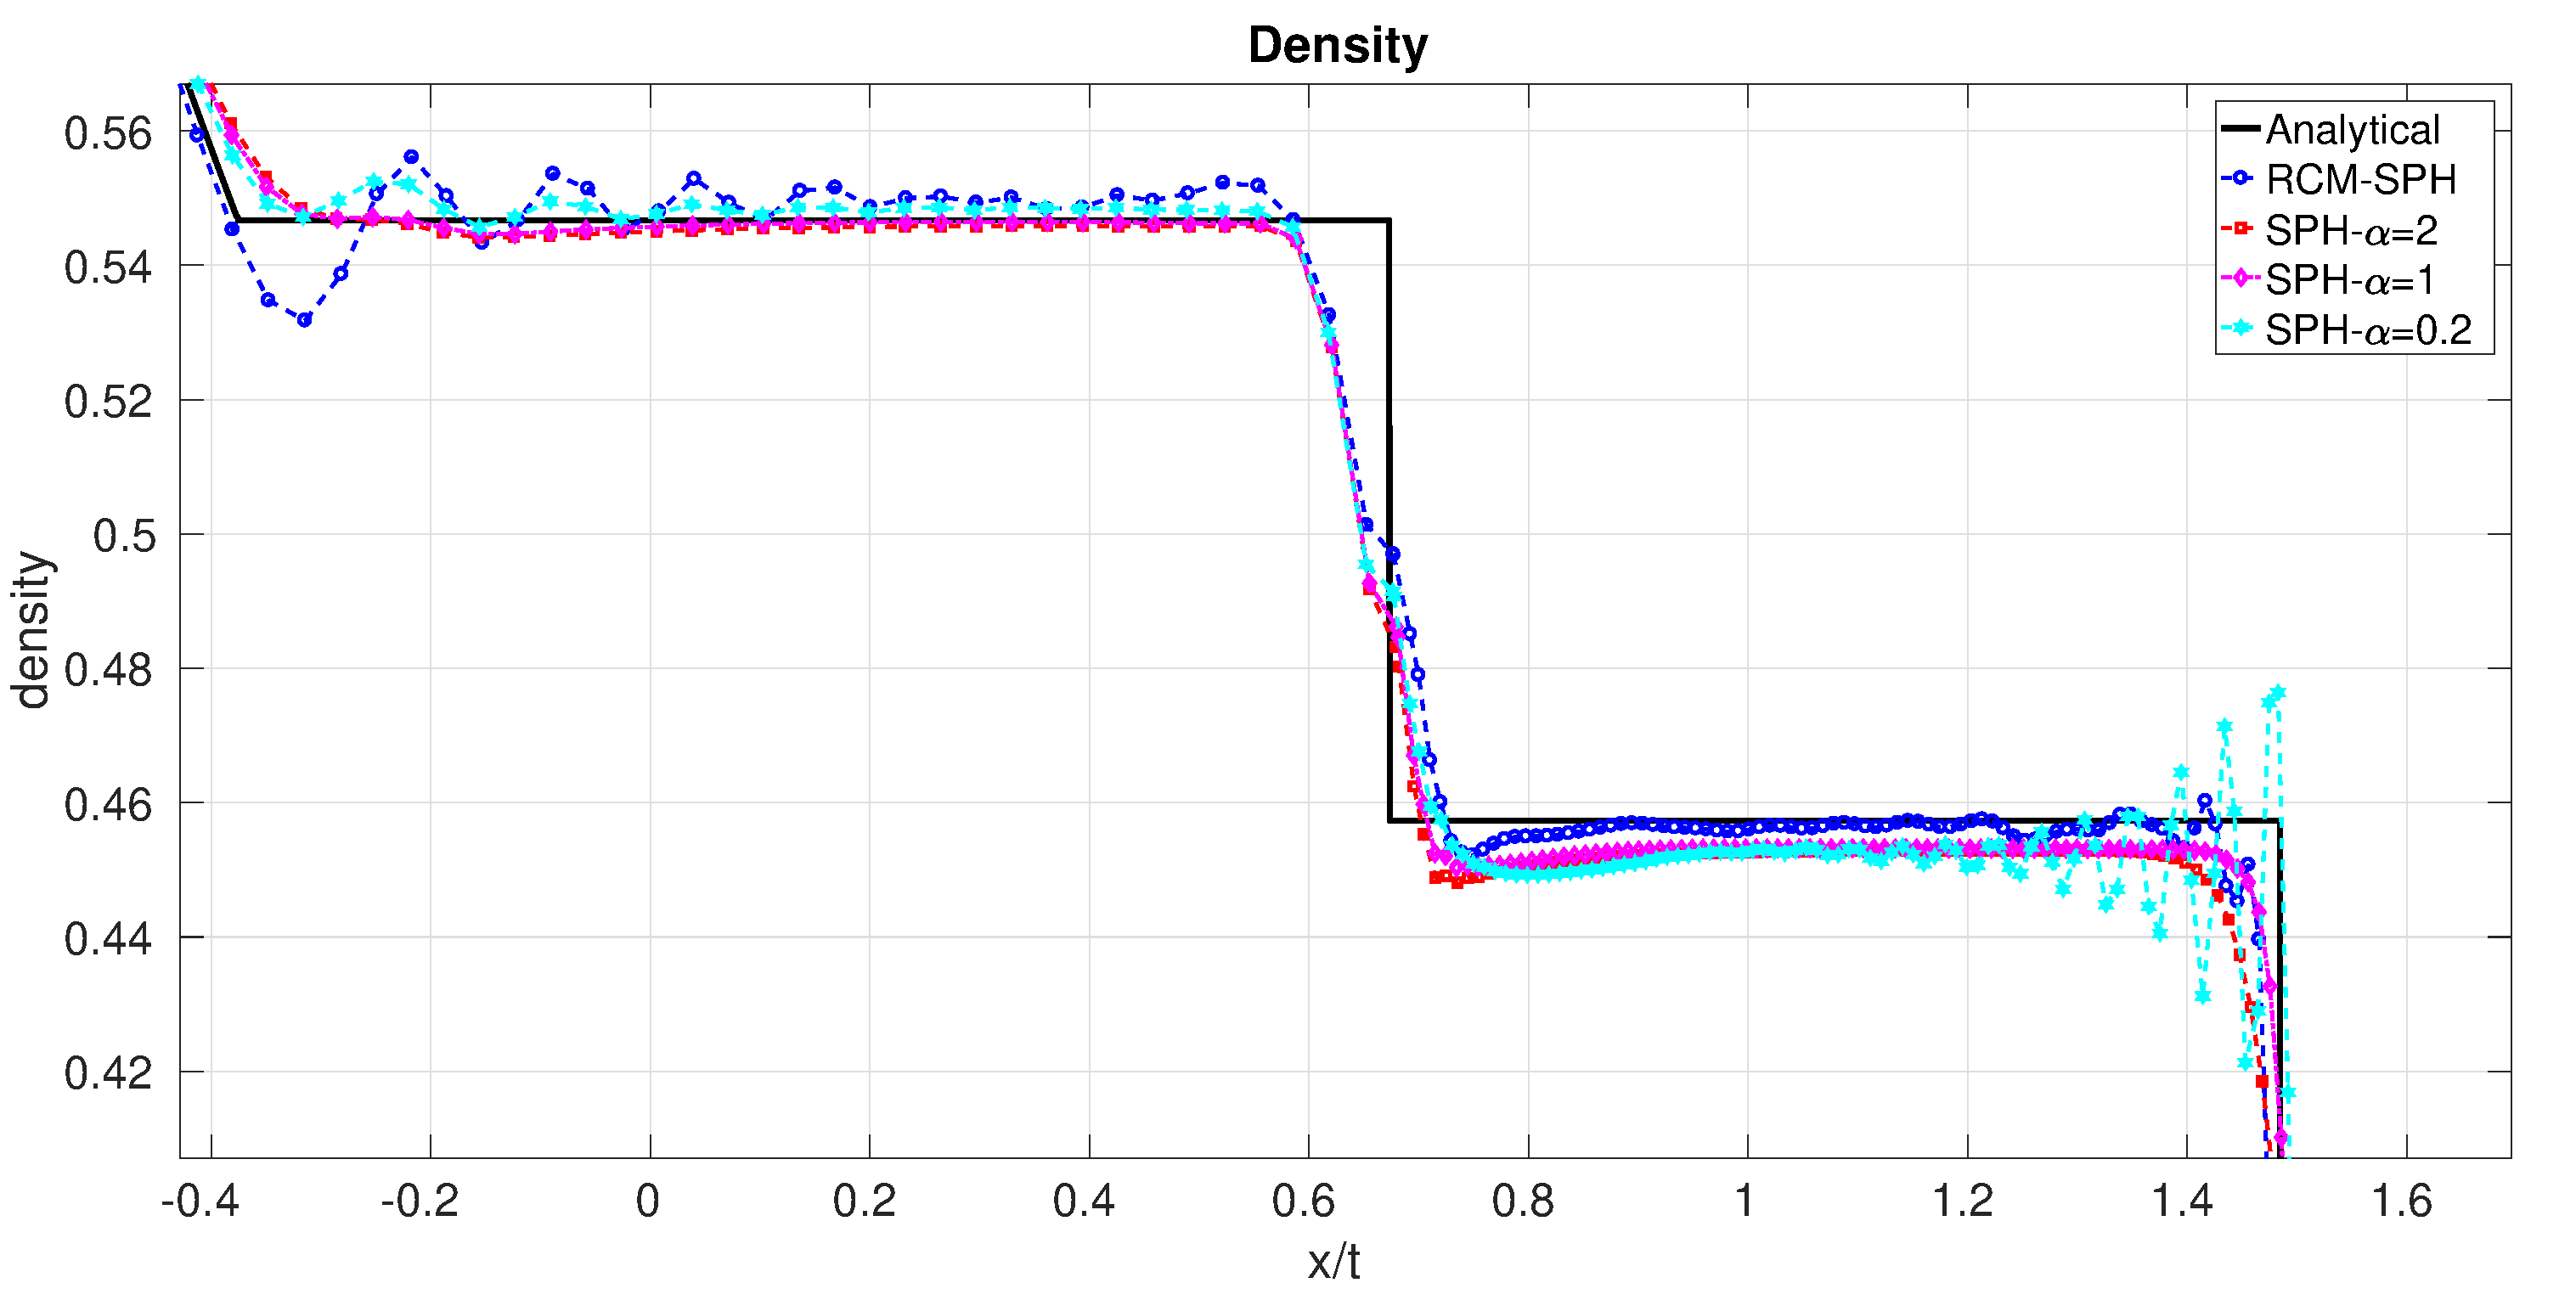
\includegraphics[width=0.99 \textwidth]{Chapter-4/Figures/Sod/RCM-Sod-SPH-alf-rho-zoom}
    \end{minipage}%
    \begin{minipage}{.495 \textwidth}
        \centering
        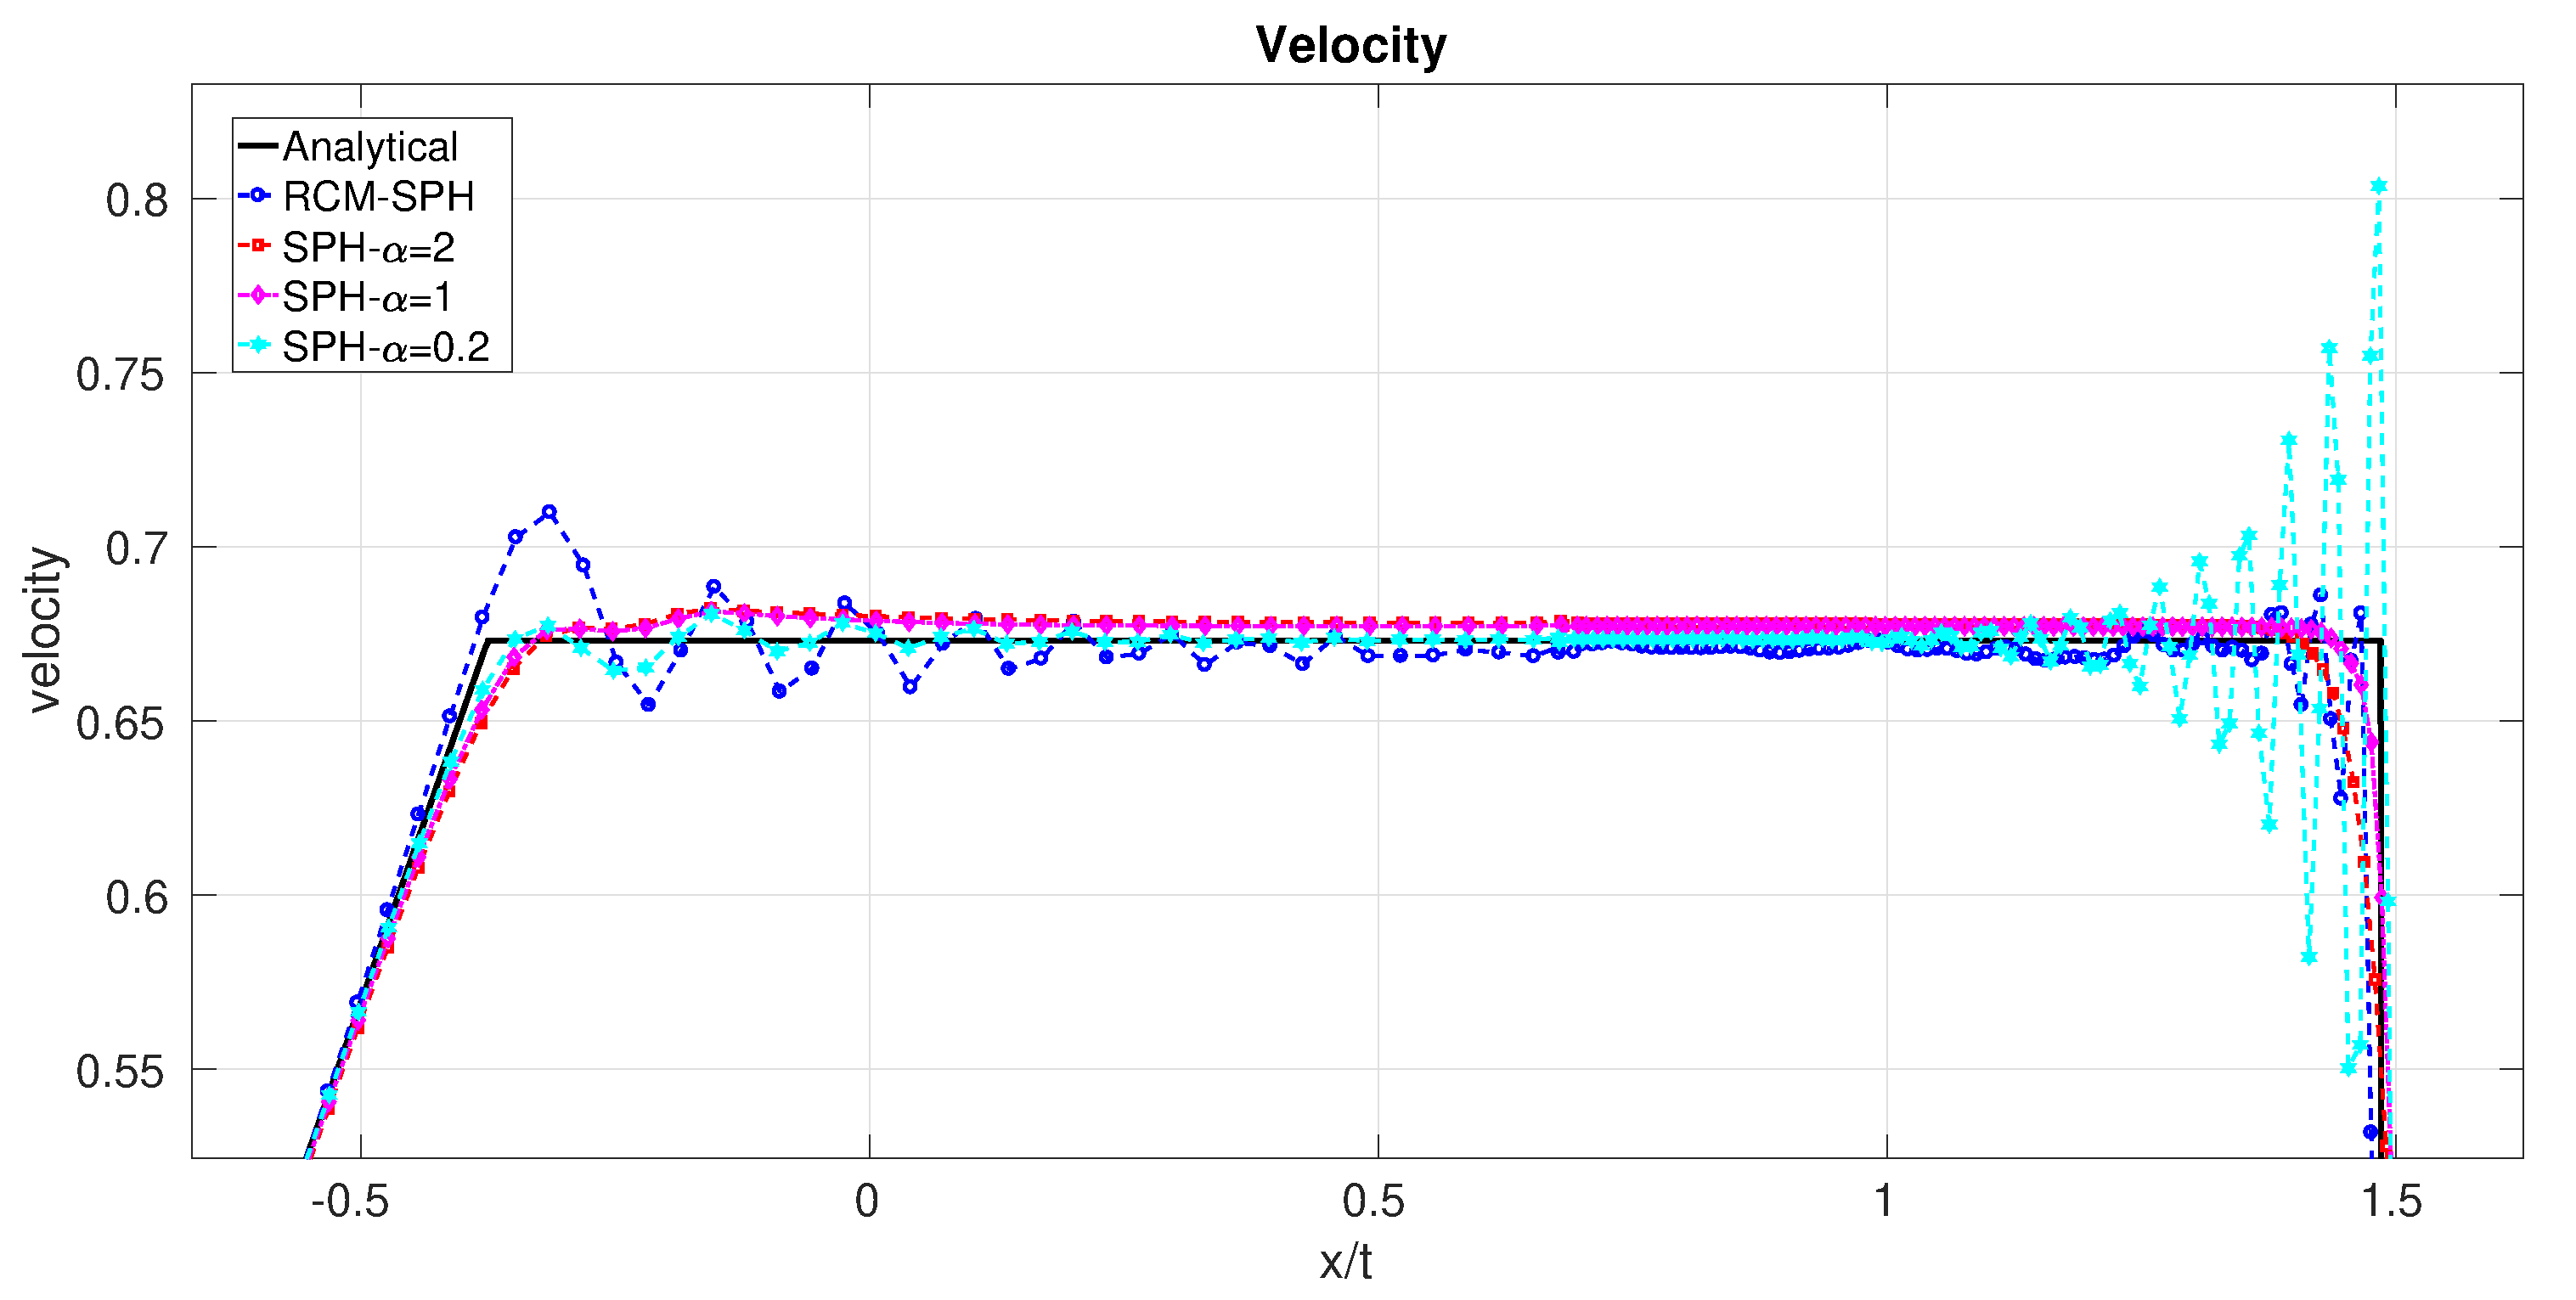
\includegraphics[width=0.99 \textwidth]{Chapter-4/Figures/Sod/RCM-Sod-SPH-alf-v-zoom}
    \end{minipage}% 
    \\
    \begin{minipage}{.495 \textwidth}
        \centering
        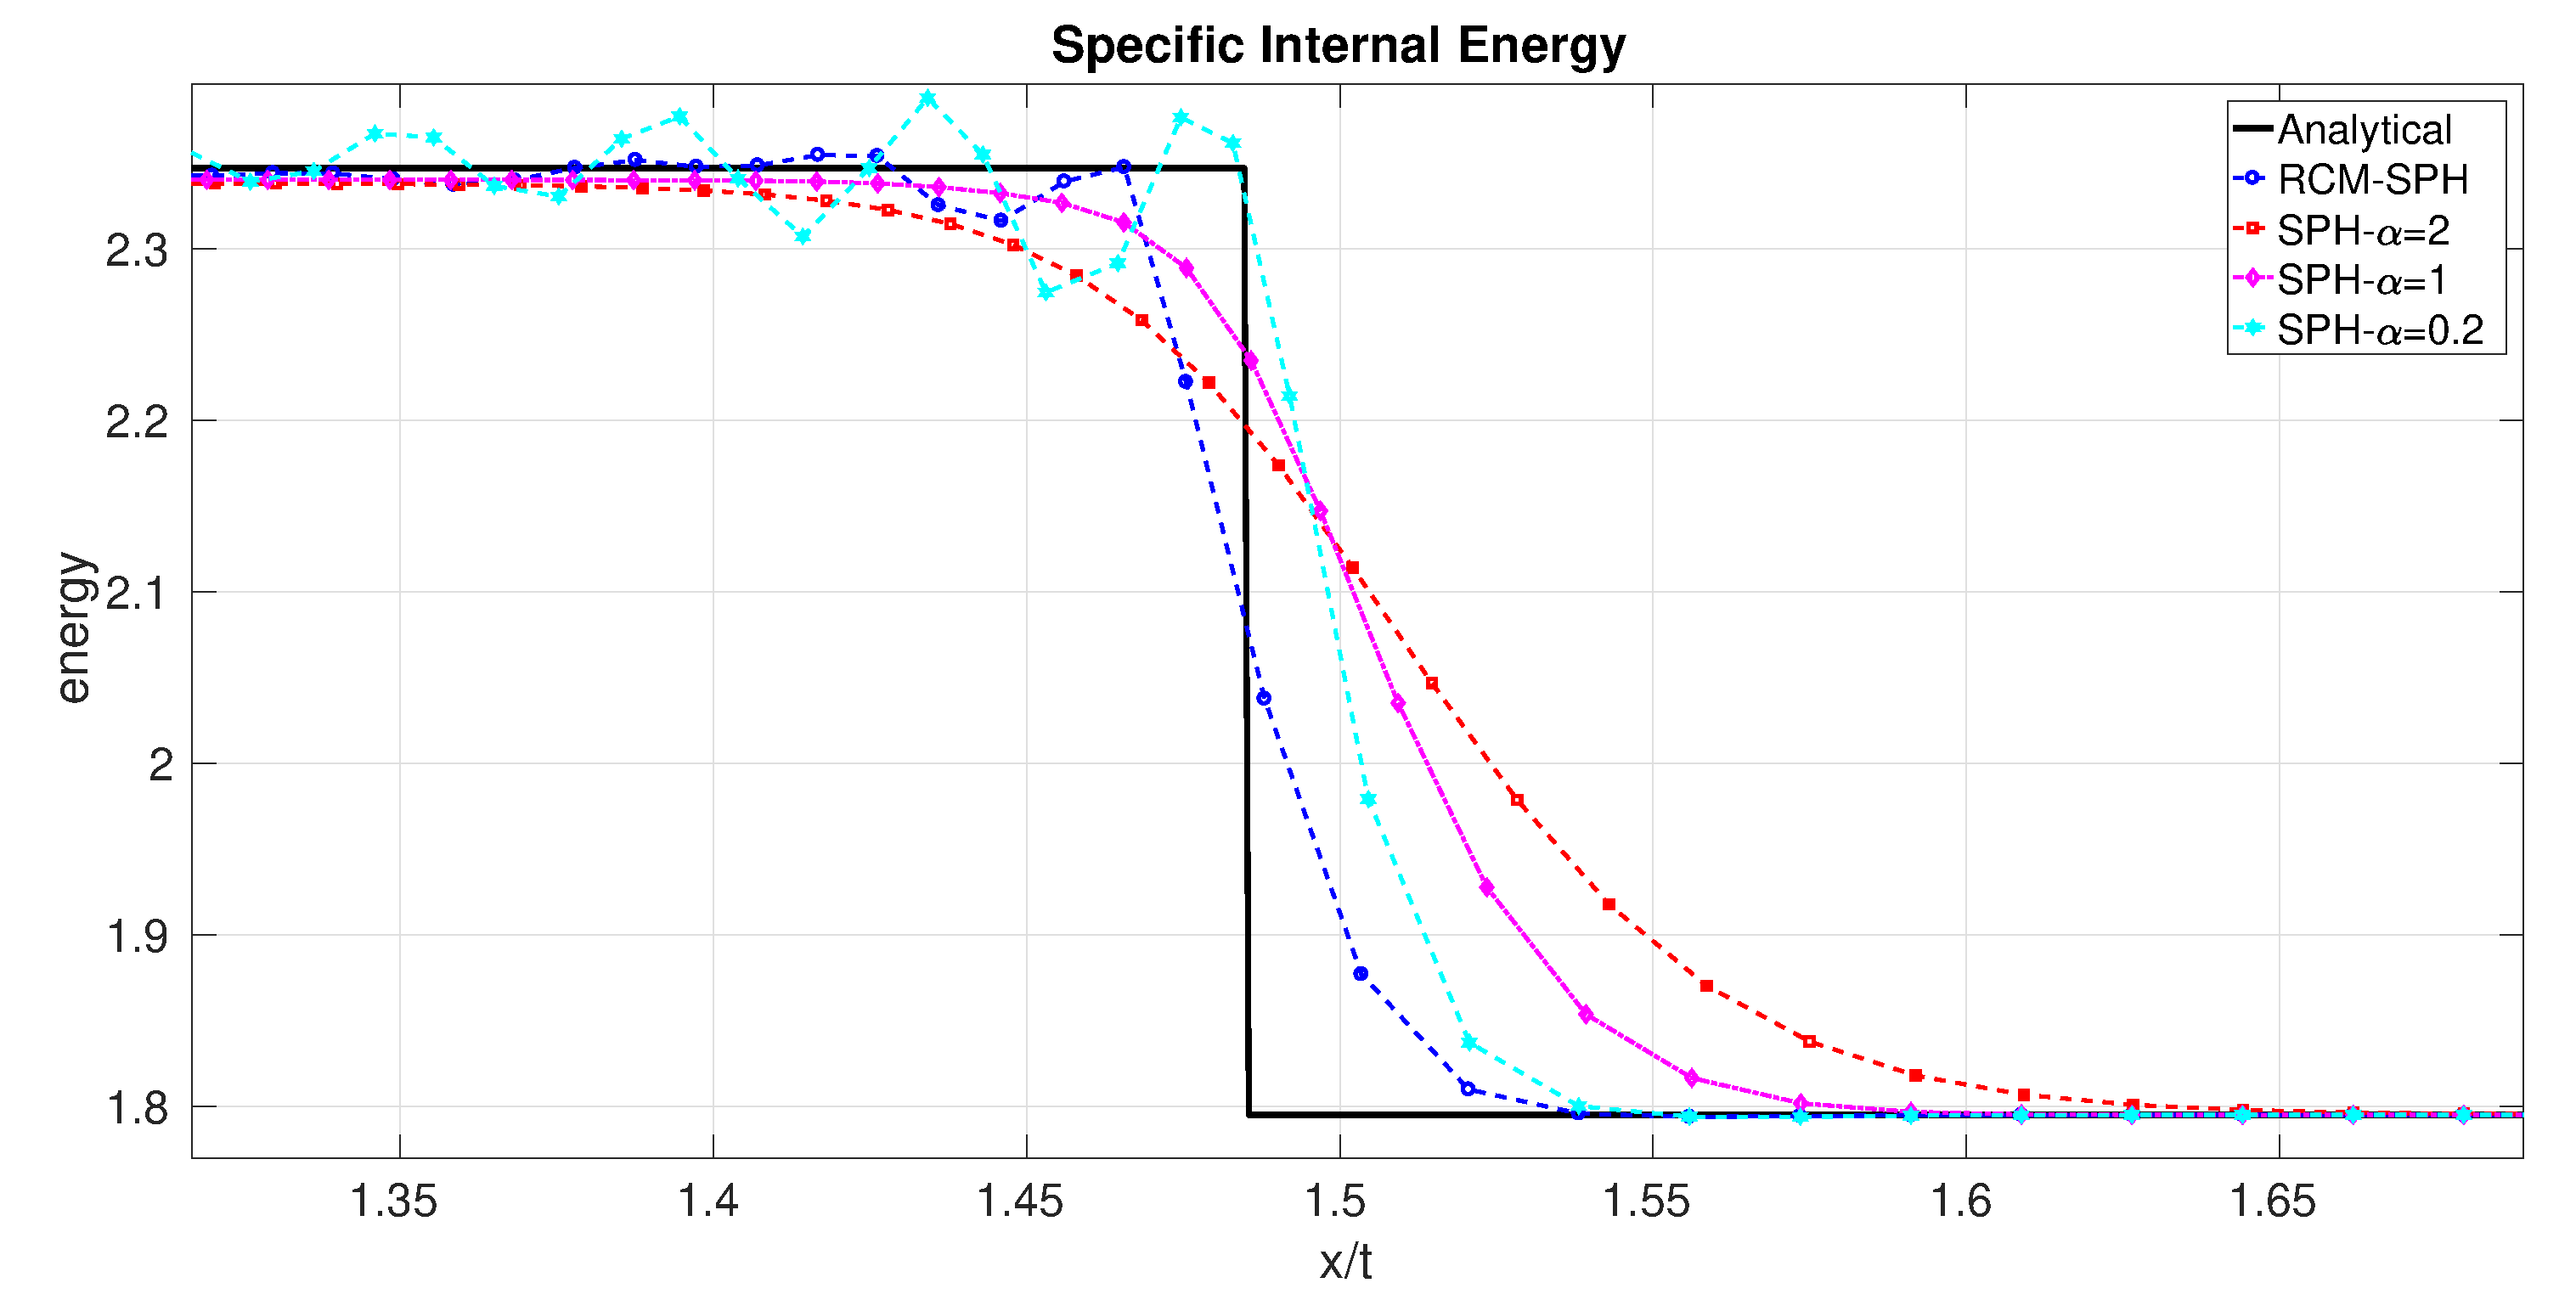
\includegraphics[width=0.99 \textwidth]{Chapter-4/Figures/Sod/RCM-Sod-SPH-alf-e-zoom}
    \end{minipage}% 
    \begin{minipage}{.495\textwidth}
        \centering
        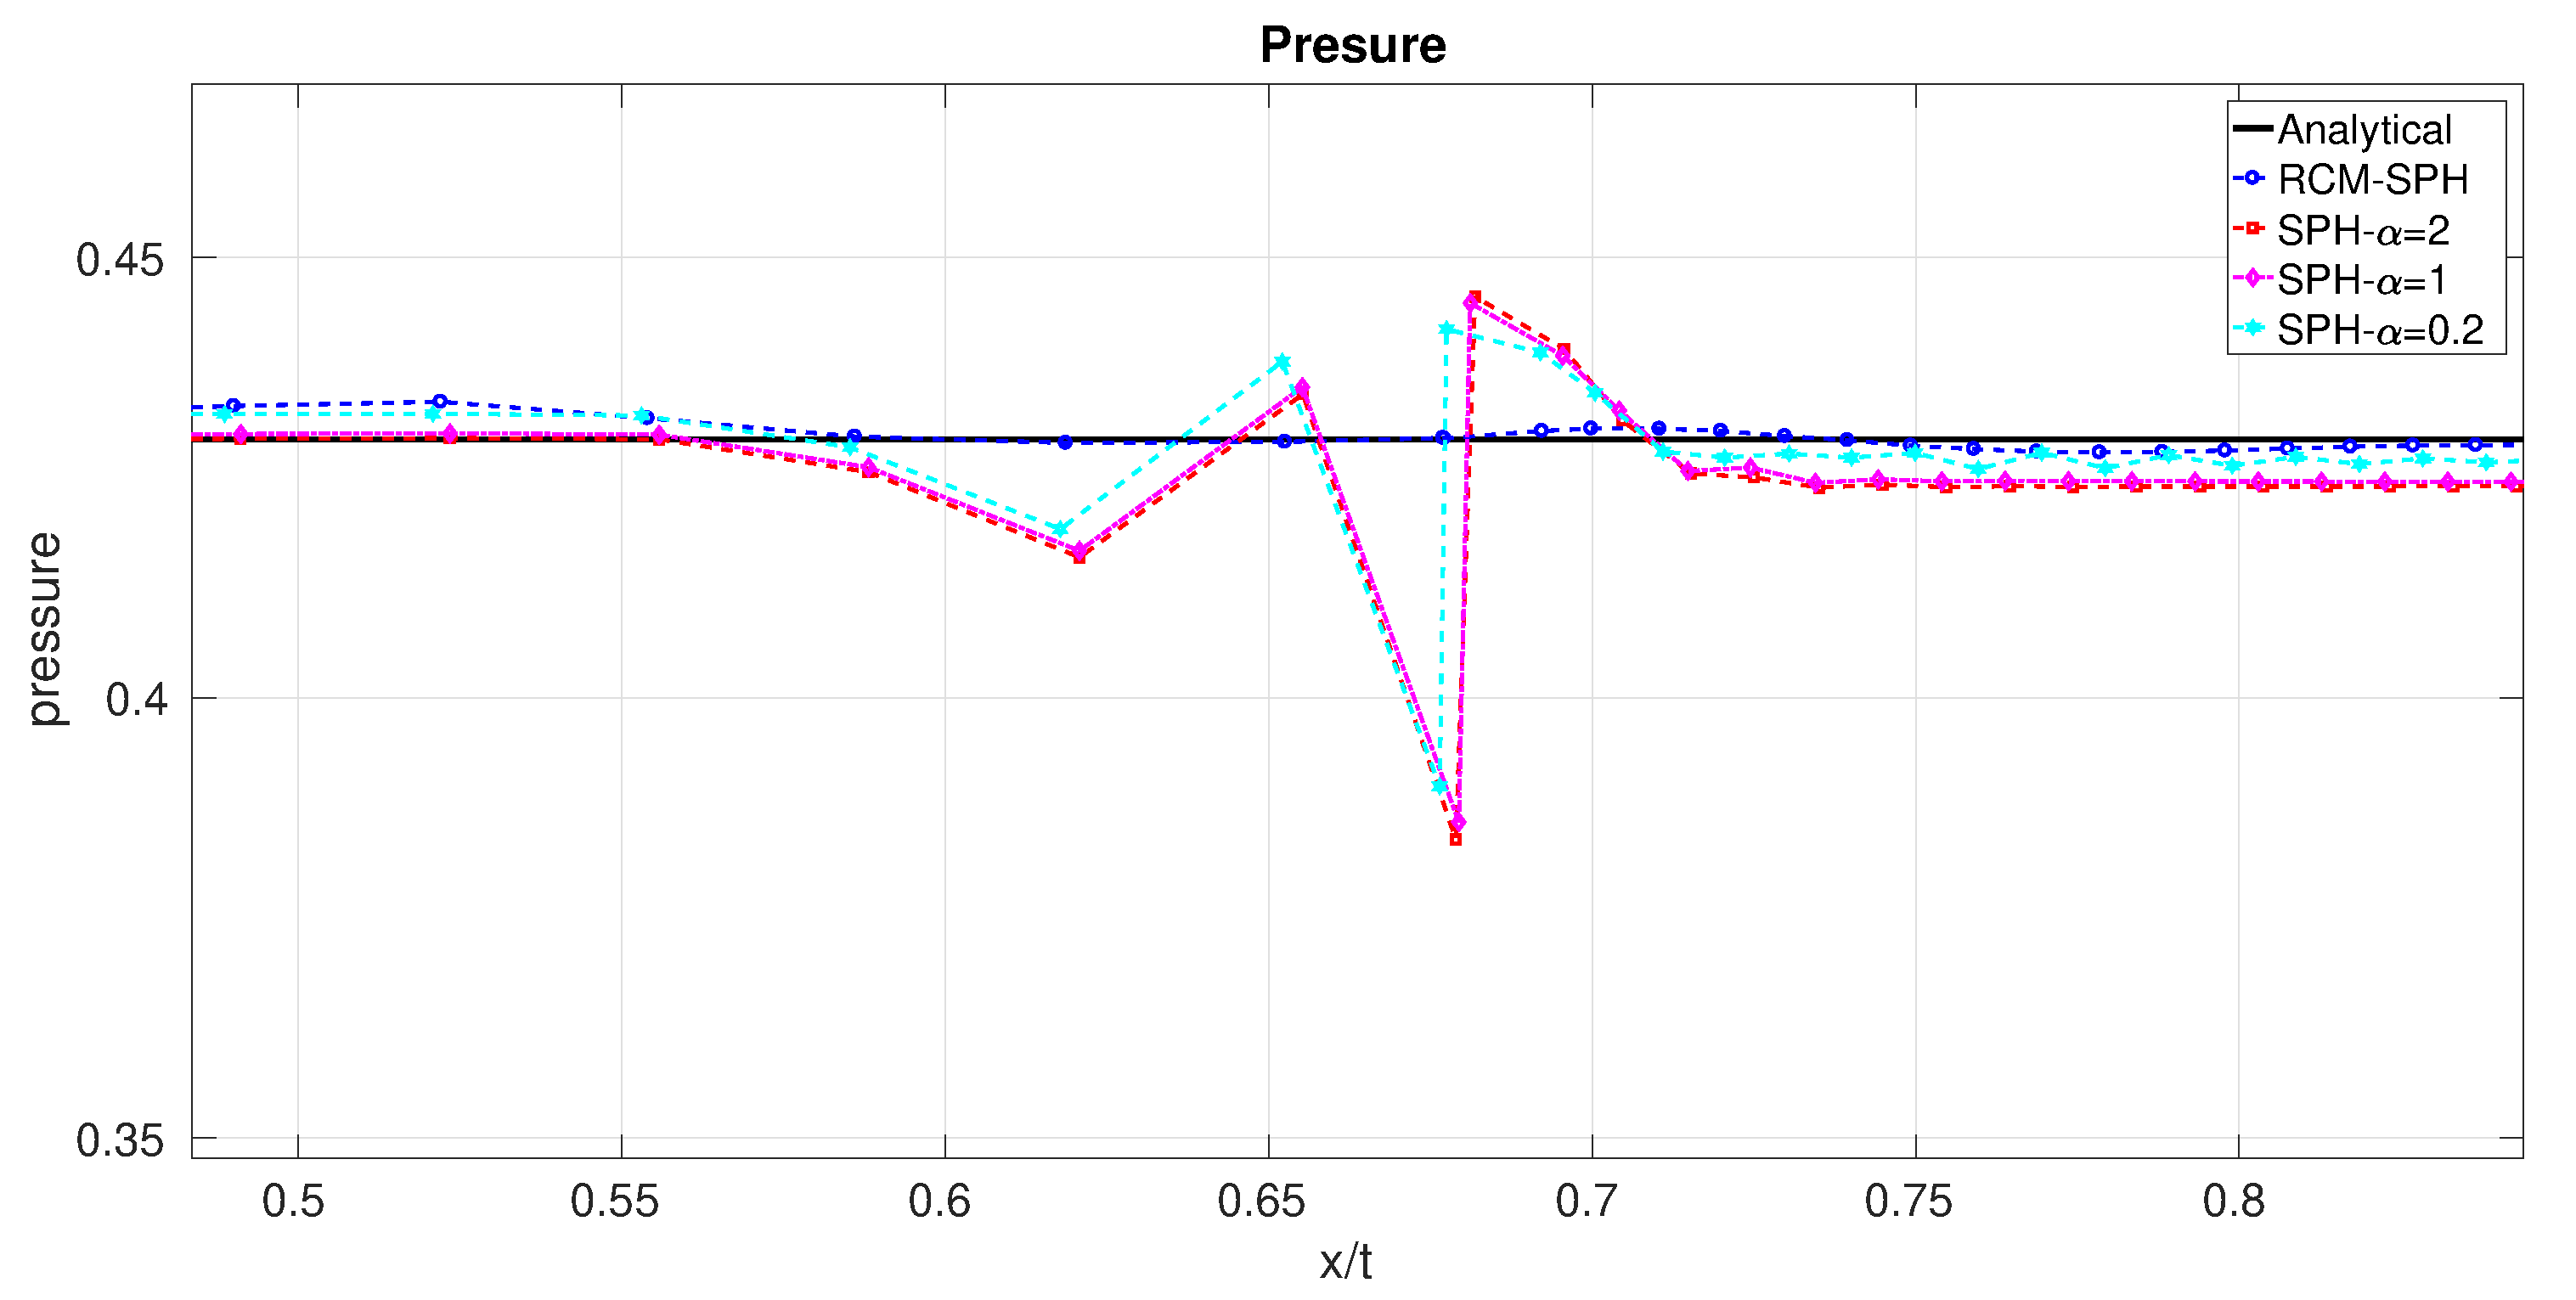
\includegraphics[width=0.99 \textwidth]{Chapter-4/Figures/Sod/RCM-Sod-SPH-alf-p-zoom}
    \end{minipage}%    
    \caption{Simulation results by RSPH and SPH with different artificial viscosity coefficients. The effect of artificial viscosity is illustrated through comparison. Artificial viscosity coefficients are chosen to always satisfy: $\beta=2\alpha$ in all SPH tests. The last four figures are zoomed views. Almost no fluctuation is observed when $\alpha=1$ and $\alpha=2$, illustrating that numerical fluctuation is completely suppressed if artificial viscosity is large enough. For density distribution obtained by RSPH, the fluctuations are more obvious in the area away from shock than those calculated by SPH with $\alpha=0.2$, implying that RSPH introduces smaller artificial viscosity than SPH with $\alpha=0.2$ in the area far away from shock. However, fluctuations around shock is much more obvious for SPH with $\alpha=0.2$ than RSPH, implying that RSPH introduces larger artificial viscosity than ``$\alpha=0.2$" around shock. To summarize, the equivalent artificial viscosity in RSPH is adaptive. Similar conclusion can be drew from zoomed view of velocity. The third zoomed view shows different degrees of smearing at the shock. The larger the artificial viscosity, the less sharp the solution at the shock. Since ``$\alpha=0.2$" is sharper than ``RSPH" at the shock, ``$\alpha=0.2$" introduces less dissipation at the shock, which is consistent with information implied by zoomed view of density and velocity. SPH with $\alpha=1.0$ and $\alpha=2.0$ introduces more dissipation than ``RSPH" in the area around the shock. The last zoomed view shows pressure around the contact discontinuity. It shows that RSPH get rid of pressure ``wiggle" around the contact discontinuity.}
    \label{fig:RCM-Sod-SPH-alf}
\end{figure}

Test 1 is simulated using standard SPH with different artificial viscosity coefficients, GSPH and RSPH. The comparison between RSPH and SPH using different artificial viscosity coefficients is shown in Fig. \ref{fig:RCM-Sod-SPH-alf}. In all simulations, the artificial viscosity $\beta$ is set to be twice of $\alpha$. For example, for the test ``$SPH-\alpha=2$", $\beta=4$. Several interesting observation are made based on the comparison between SPH and RSPH.
First of all, dissipation (introduced by artificial viscosity in these tests) can decays the numerical fluctuations. Numerical fluctuations are suppressed completely when large enough dissipation is introduced, for example, by using sufficiently large artificial viscosity coefficients.
%The mechanism for SPH to reduce (or completely get rid of) fluctuations should be completely different from that of new adaptive method of smoothing length. 
%The new adaptive method, reduces the sources of such fluctuations.
Secondly, the equivalent artificial viscosity coefficients introduced by RSPH varies adaptively.
As shown in Fig. \ref{fig:RCM-Sod-SPH-alf}, RSPH assigns smaller artificial viscosity coefficients (equivalent $\alpha$ much less then 0.2) at the area far away from shock and sufficient large artificial viscosity coefficients (equivalent $\alpha$ is about 1.0) around the shock. So RSPH is actually more adaptive than SPH. This feature is very desirable not only because it could eliminate parameterization and hence user intervention associated with artificial viscosity coefficients but also because it avoids introducing excessive artificial viscosity when unnecessary.
Thirdly, RSPH introduces less smearing of the shock discontinuity compared with SPH using most commonly adopted artificial viscosity coefficients ($\alpha=1.0$, $\beta=2.0$). Recall that RCM is able to resolve discontinuities as true discontinuity. RSPH, even though still smears the discontinuity in some degree, introduces much less smearing.
The last but not the least, the pressure ``wiggle" around contact discontinuity is completely eliminated by RSPH. It has been shown that thermal conduction is essential to mitigate the spurious pressure ``wiggle" at contact discontinuity in SPH \citep{monaghan1997sph, sigalotti2006shock, price2008modelling, price2012smoothed}. As for GSPH, it is reported that an implicit thermal conduction is introduced by Godunov's scheme and help suppress the anomaly \citep{puri2014approximate}. Even though, the ``wiggle" still visible in pressure distribution and velocity distribution of GSPH simulation results (for example, see figures in \citep{puri2014comparison}) and RSPH simulation results of other tests (see section \ref{sec:comprehensive-1d-tests}). ``Wiggle" in test 1, however, is completely eliminated by both GSPH and RSPH.

\begin{figure}[htp]
    \centering
    \begin{minipage}{.495\textwidth}
        \centering
        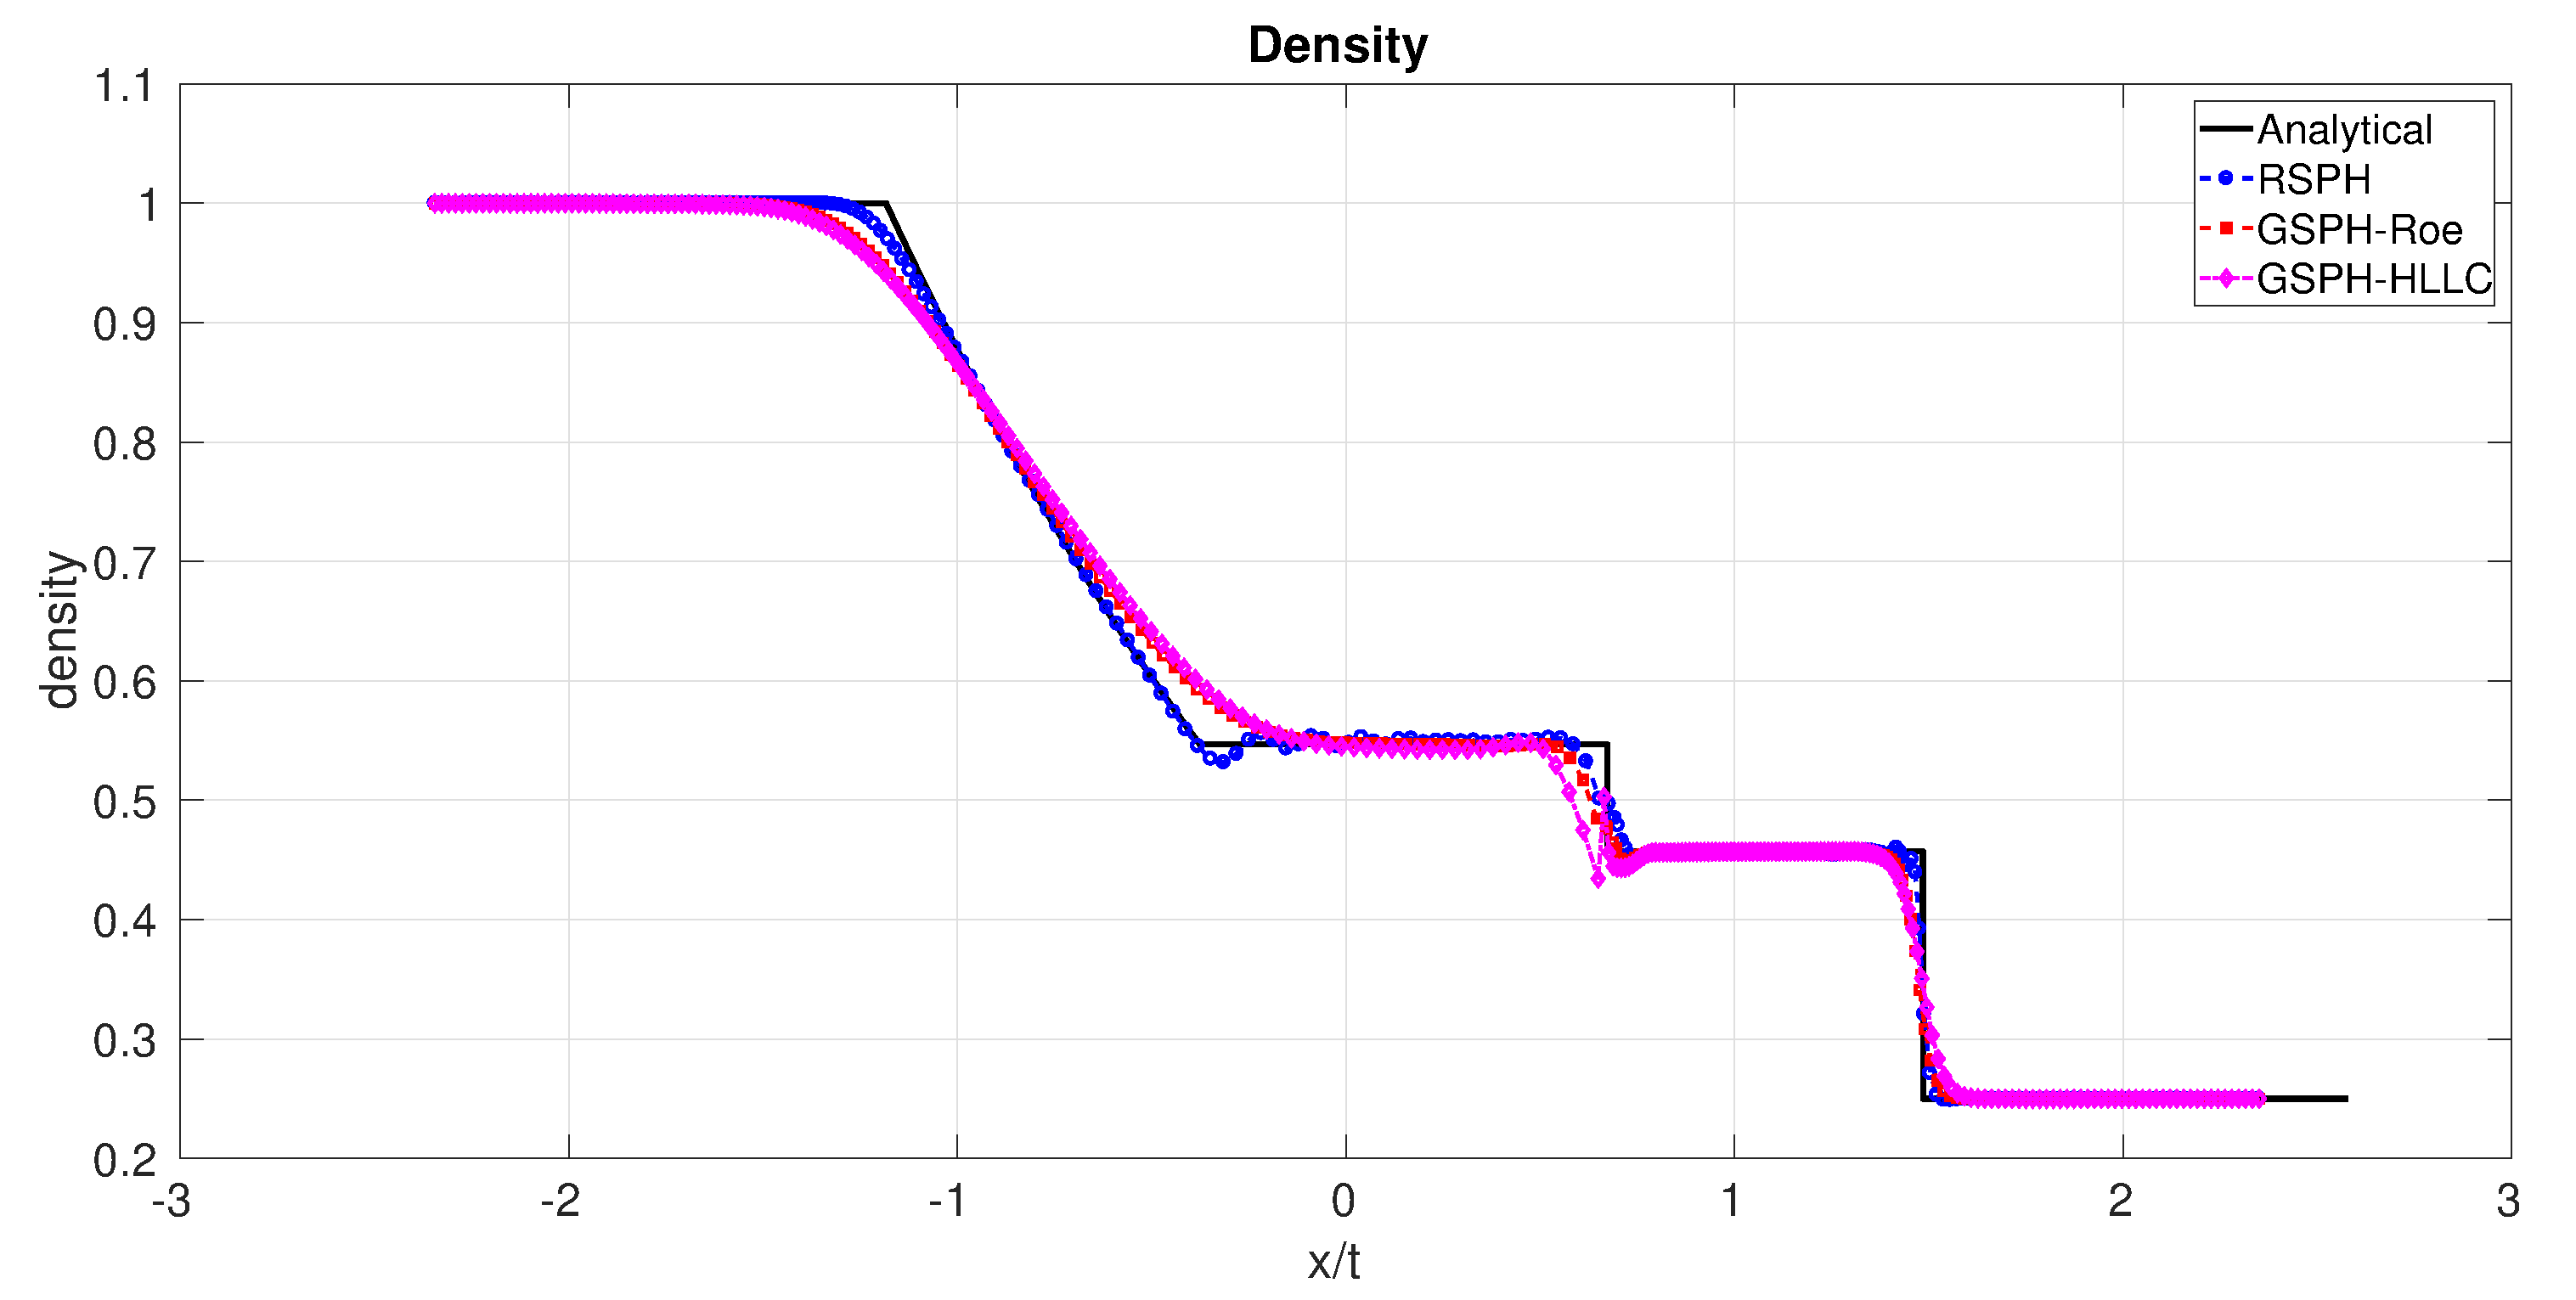
\includegraphics[width=0.99 \textwidth]{Chapter-4/Figures/Sod/RCM-Sod-GSPH-compare-rho}
    \end{minipage}%
    \begin{minipage}{.495 \textwidth}
        \centering
        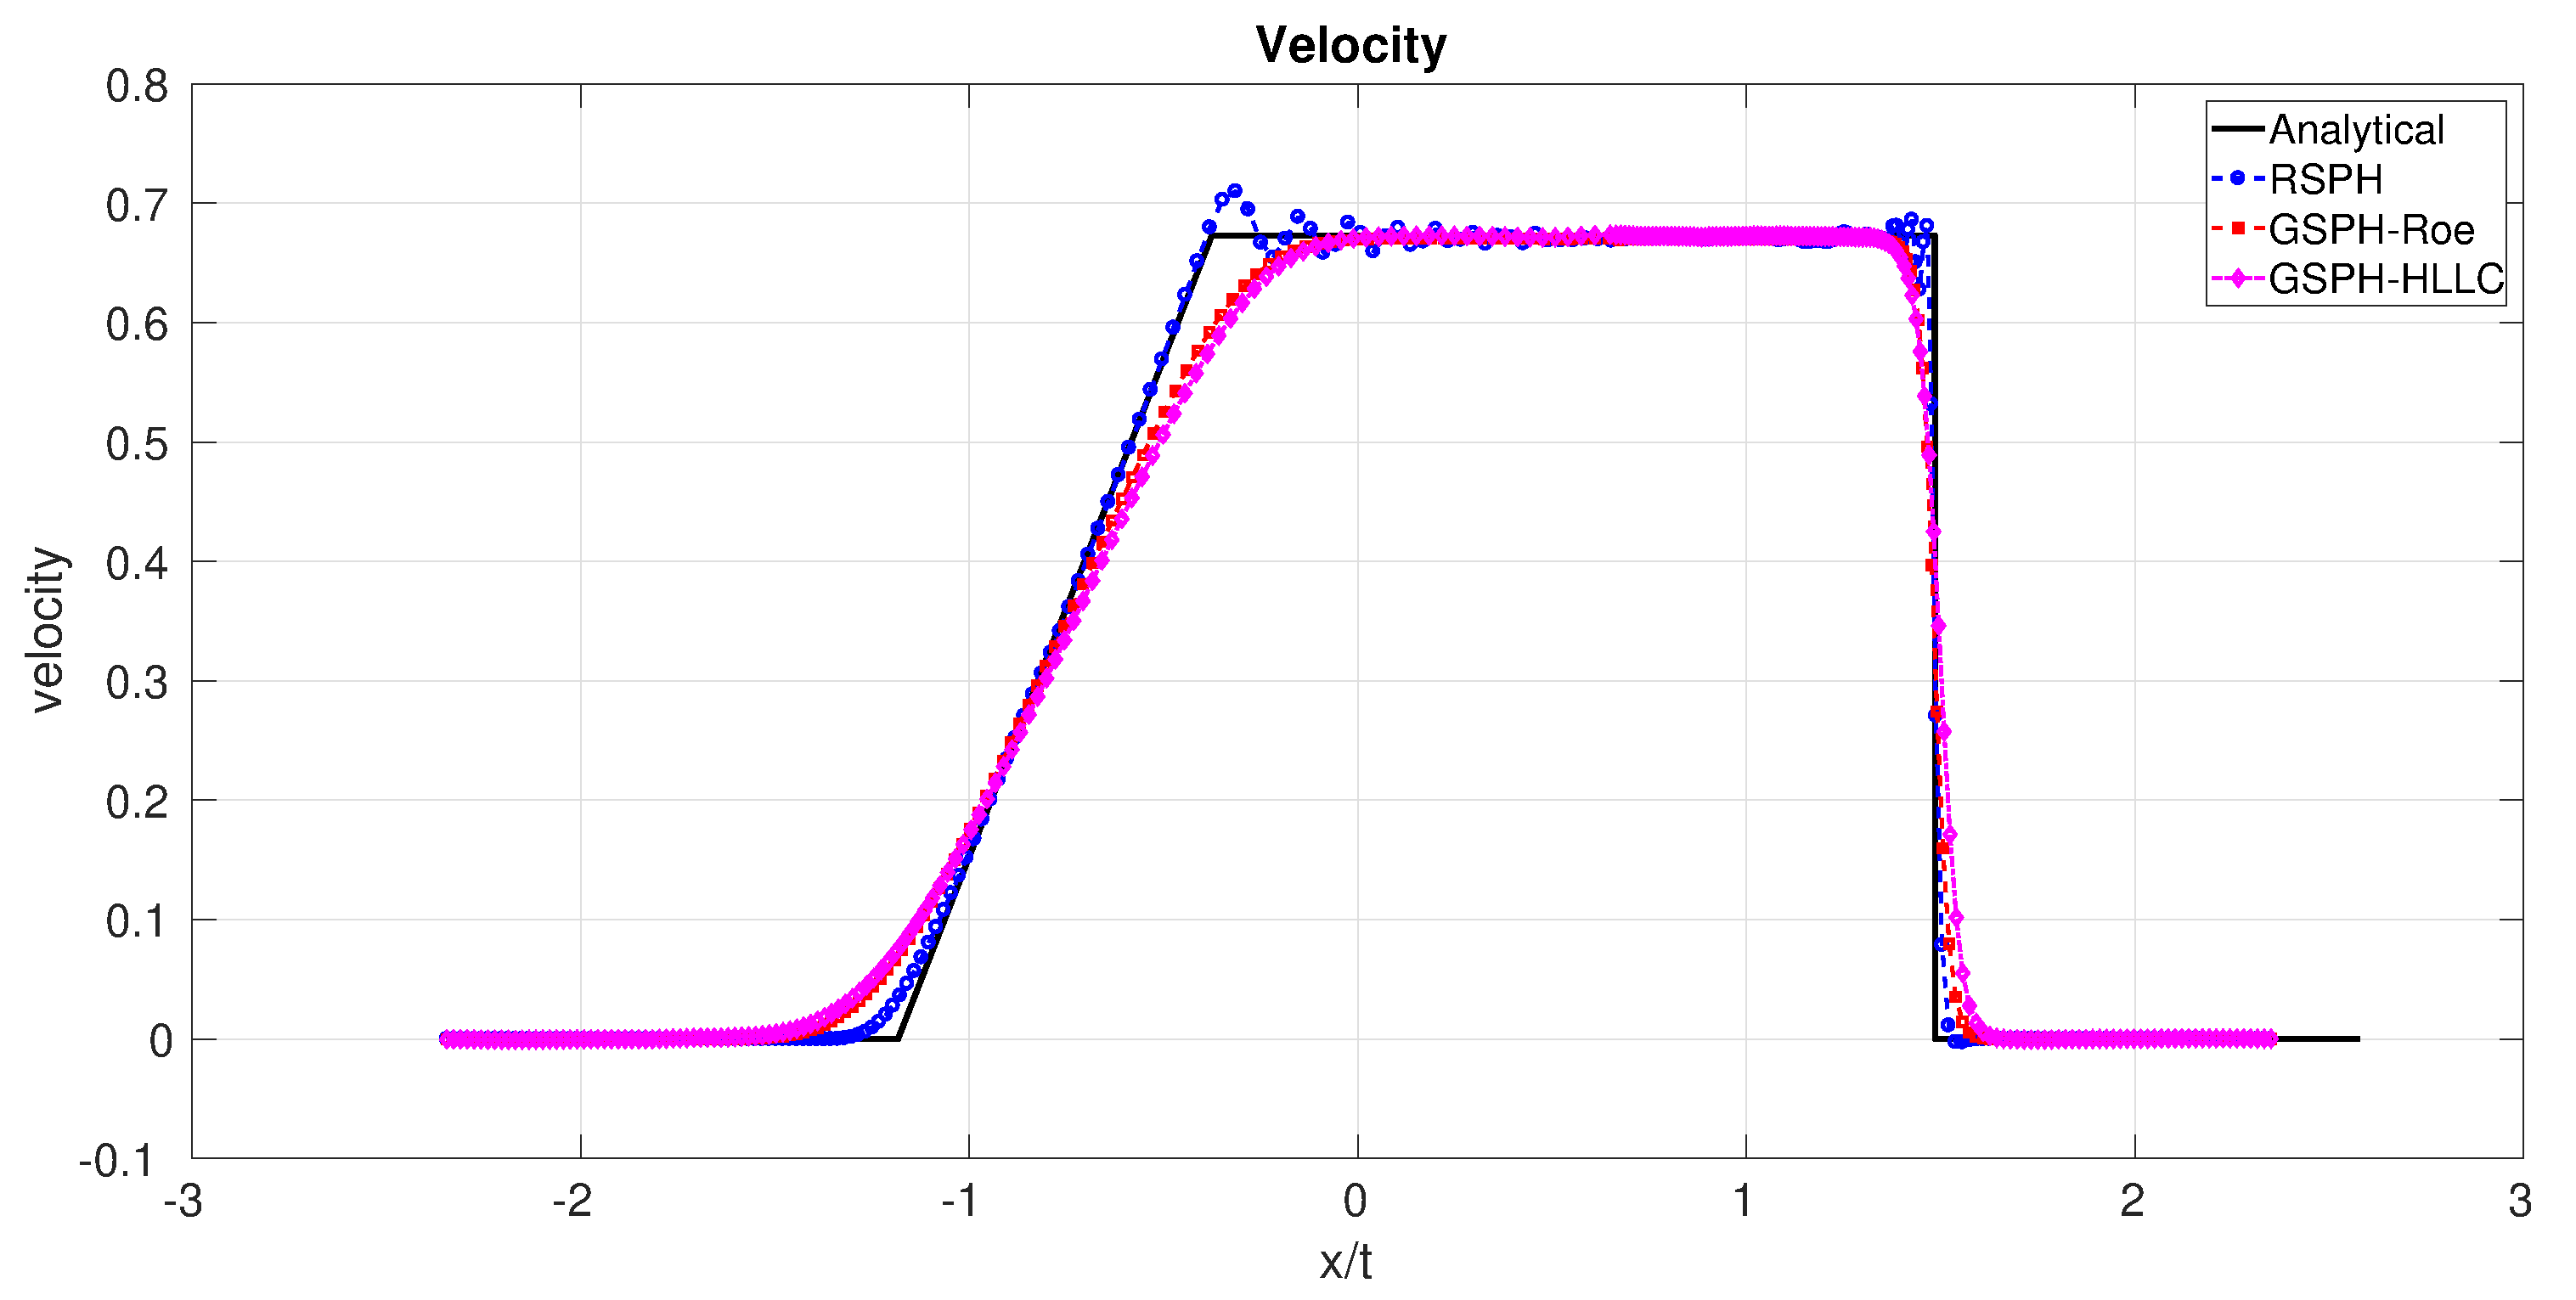
\includegraphics[width=0.99 \textwidth]{Chapter-4/Figures/Sod/RCM-Sod-GSPH-compare-v}
    \end{minipage}%
    \\
    \begin{minipage}{.495\textwidth}
        \centering
        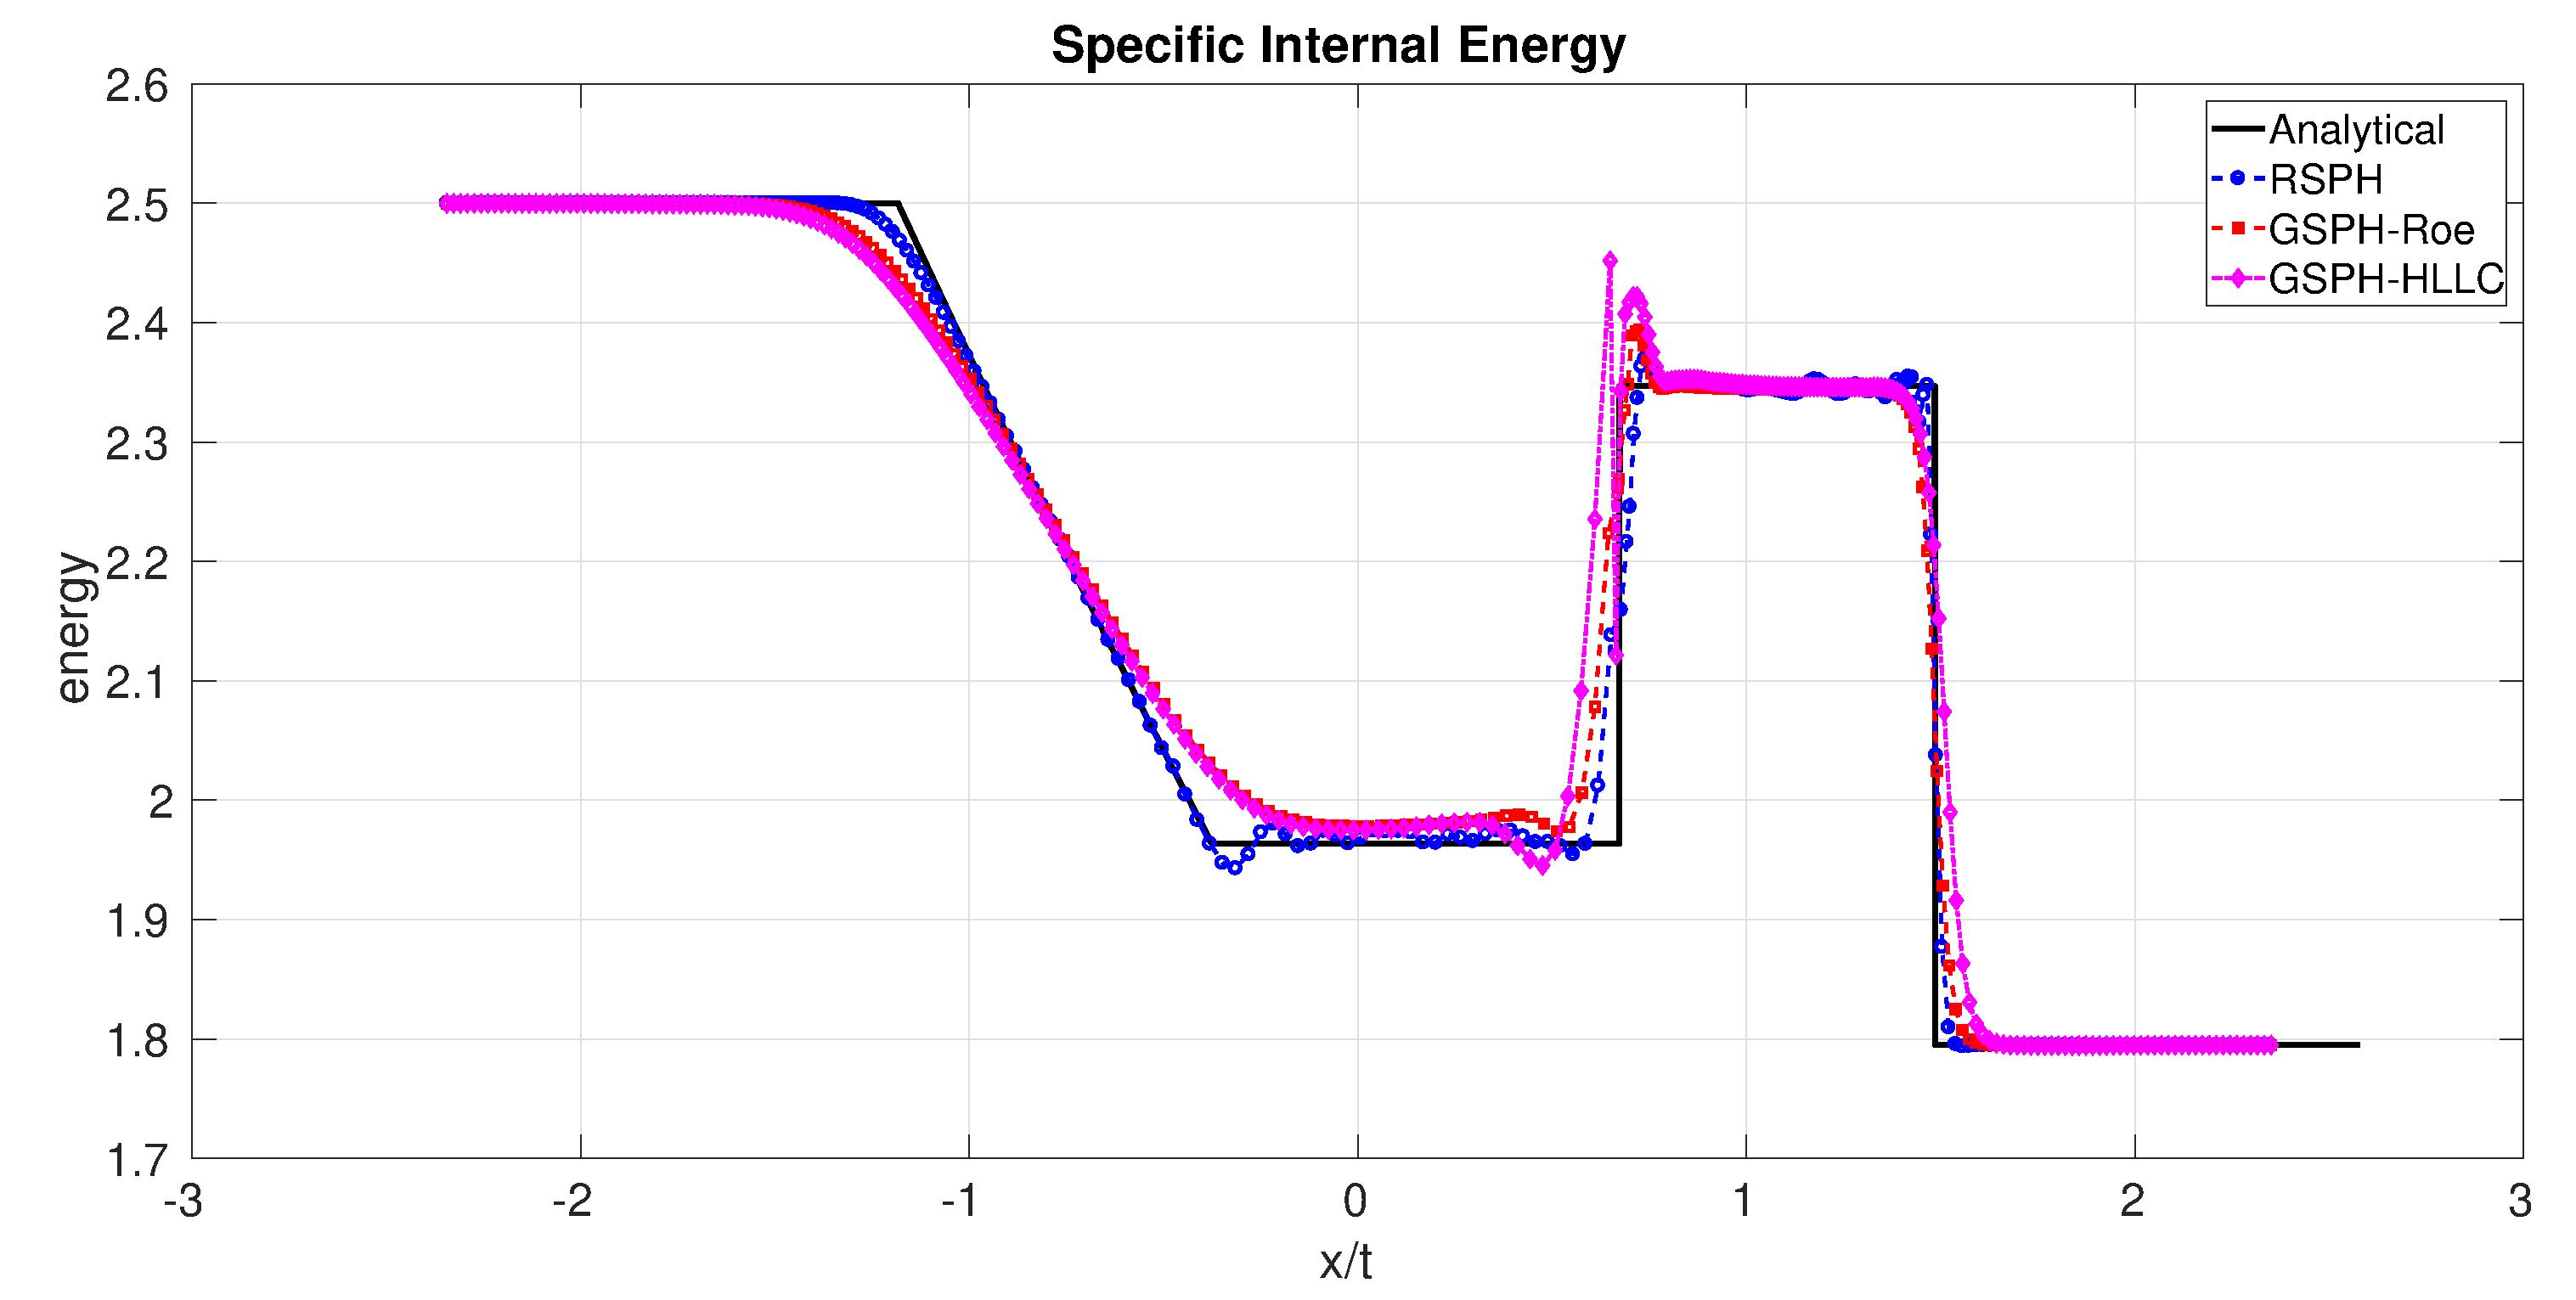
\includegraphics[width=0.99 \textwidth]{Chapter-4/Figures/Sod/RCM-Sod-GSPH-compare-e}
    \end{minipage}%
    \begin{minipage}{.495 \textwidth}
        \centering
        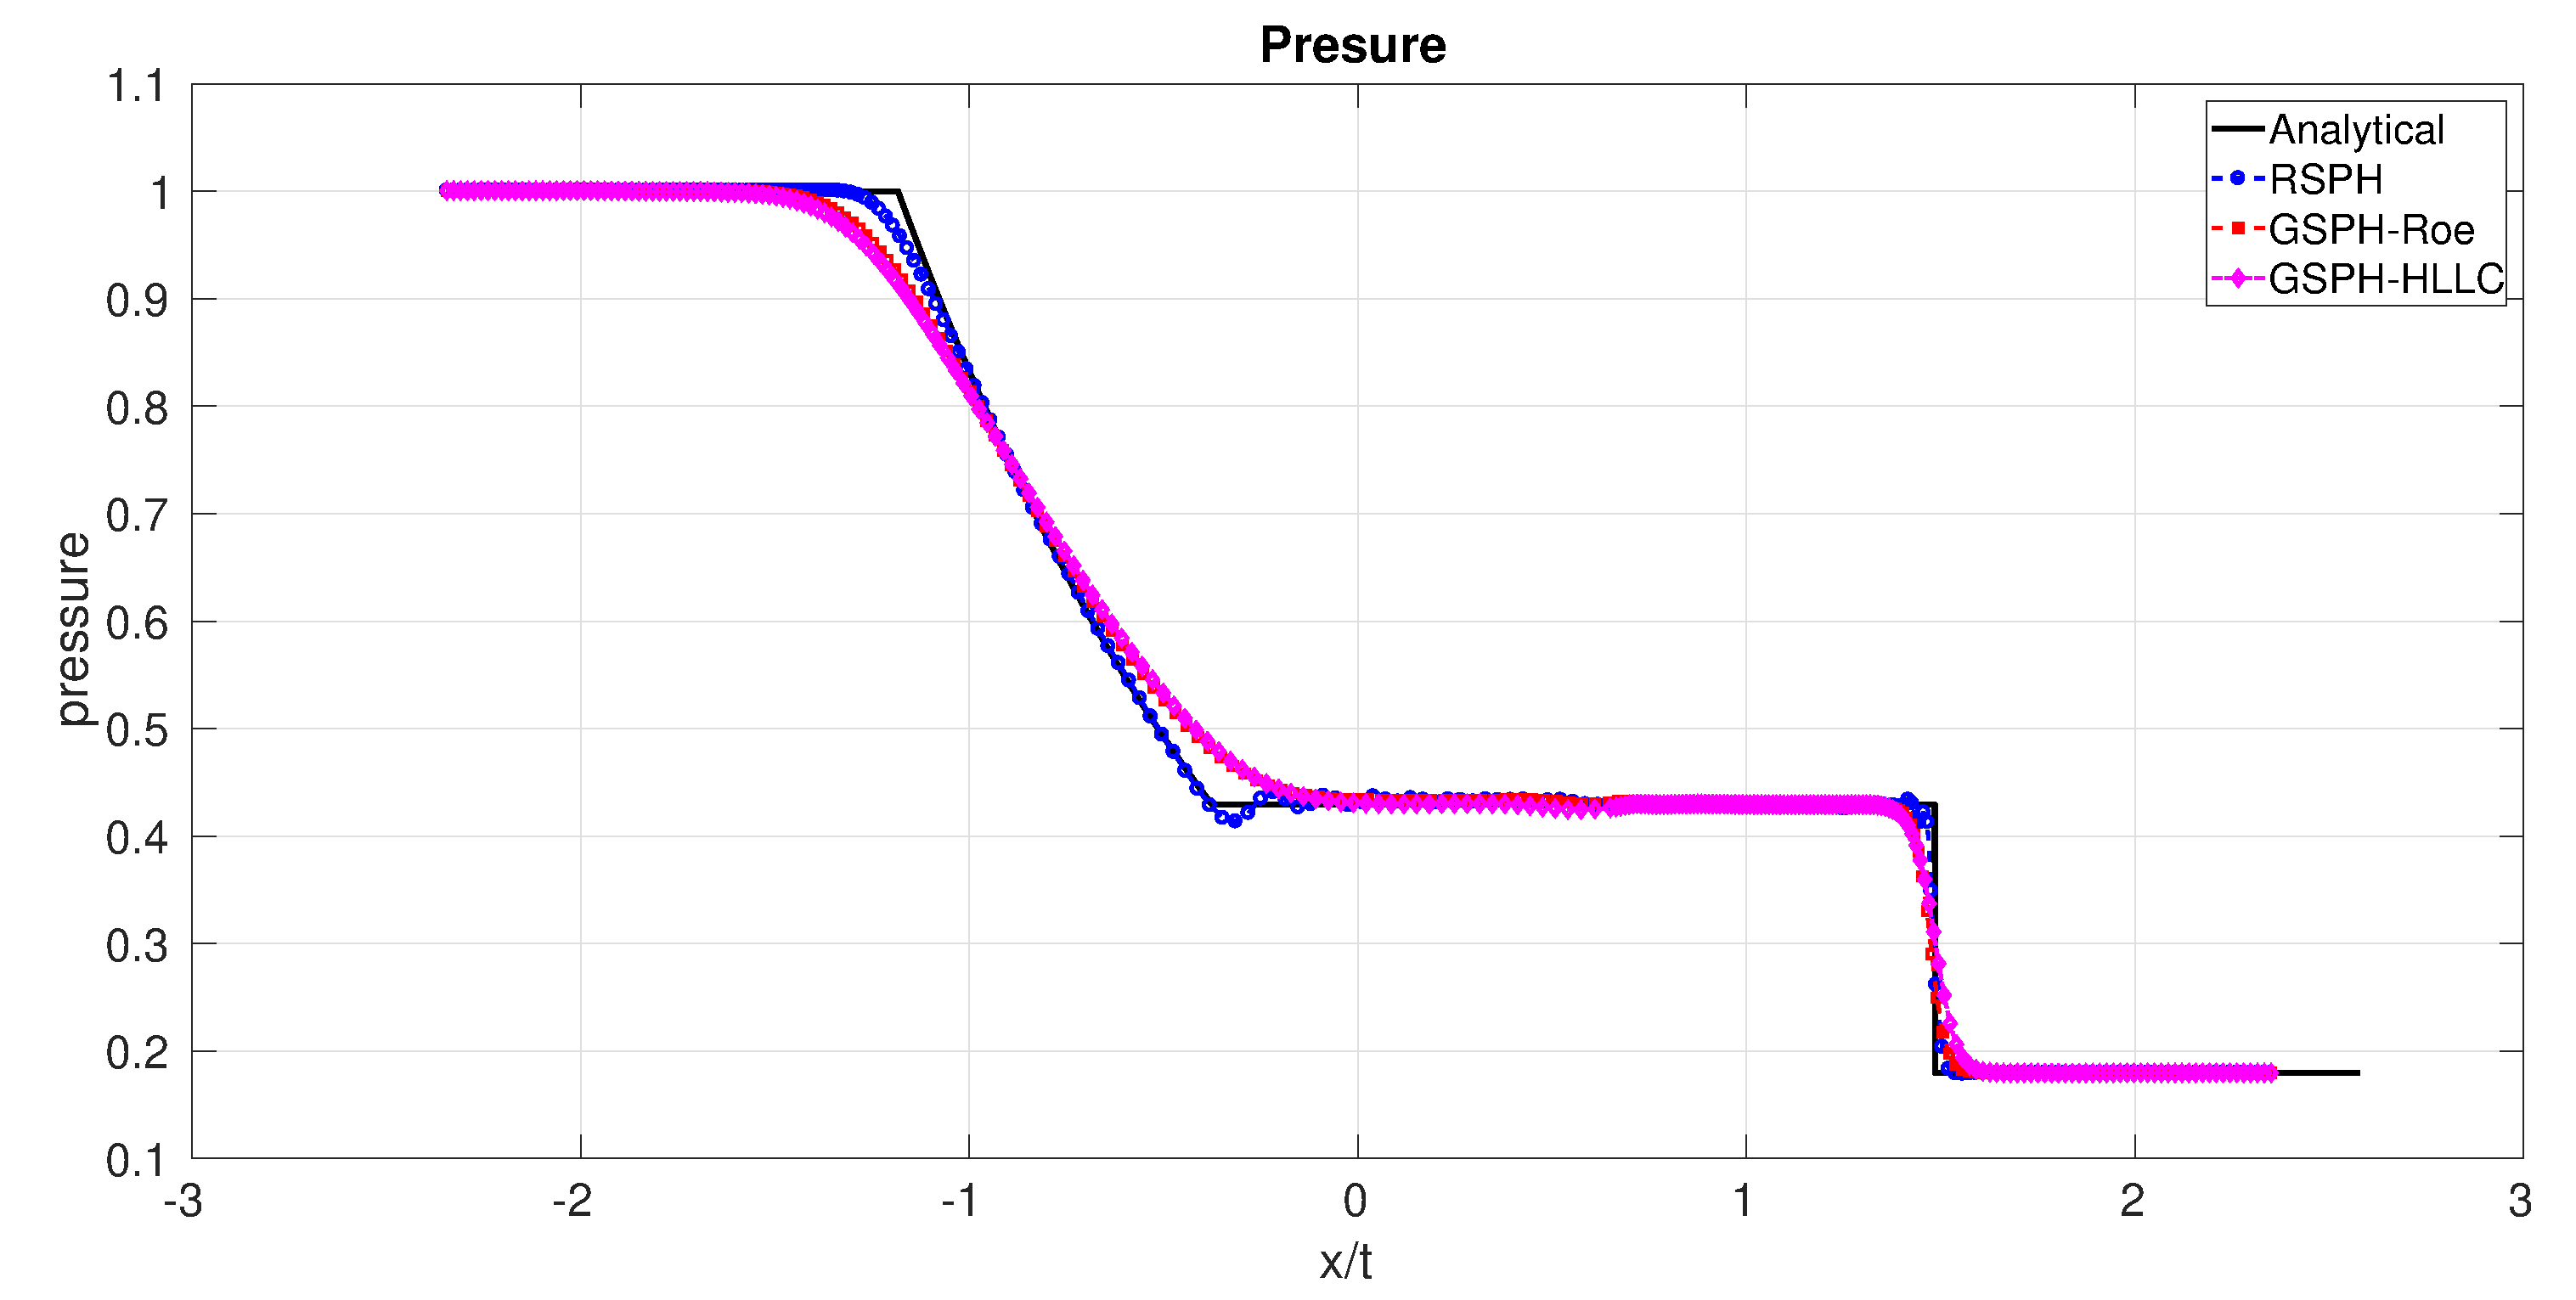
\includegraphics[width=0.99 \textwidth]{Chapter-4/Figures/Sod/RCM-Sod-GSPH-compare-p}
    \end{minipage}% 
    \\
    \begin{minipage}{.495\textwidth}
        \centering
        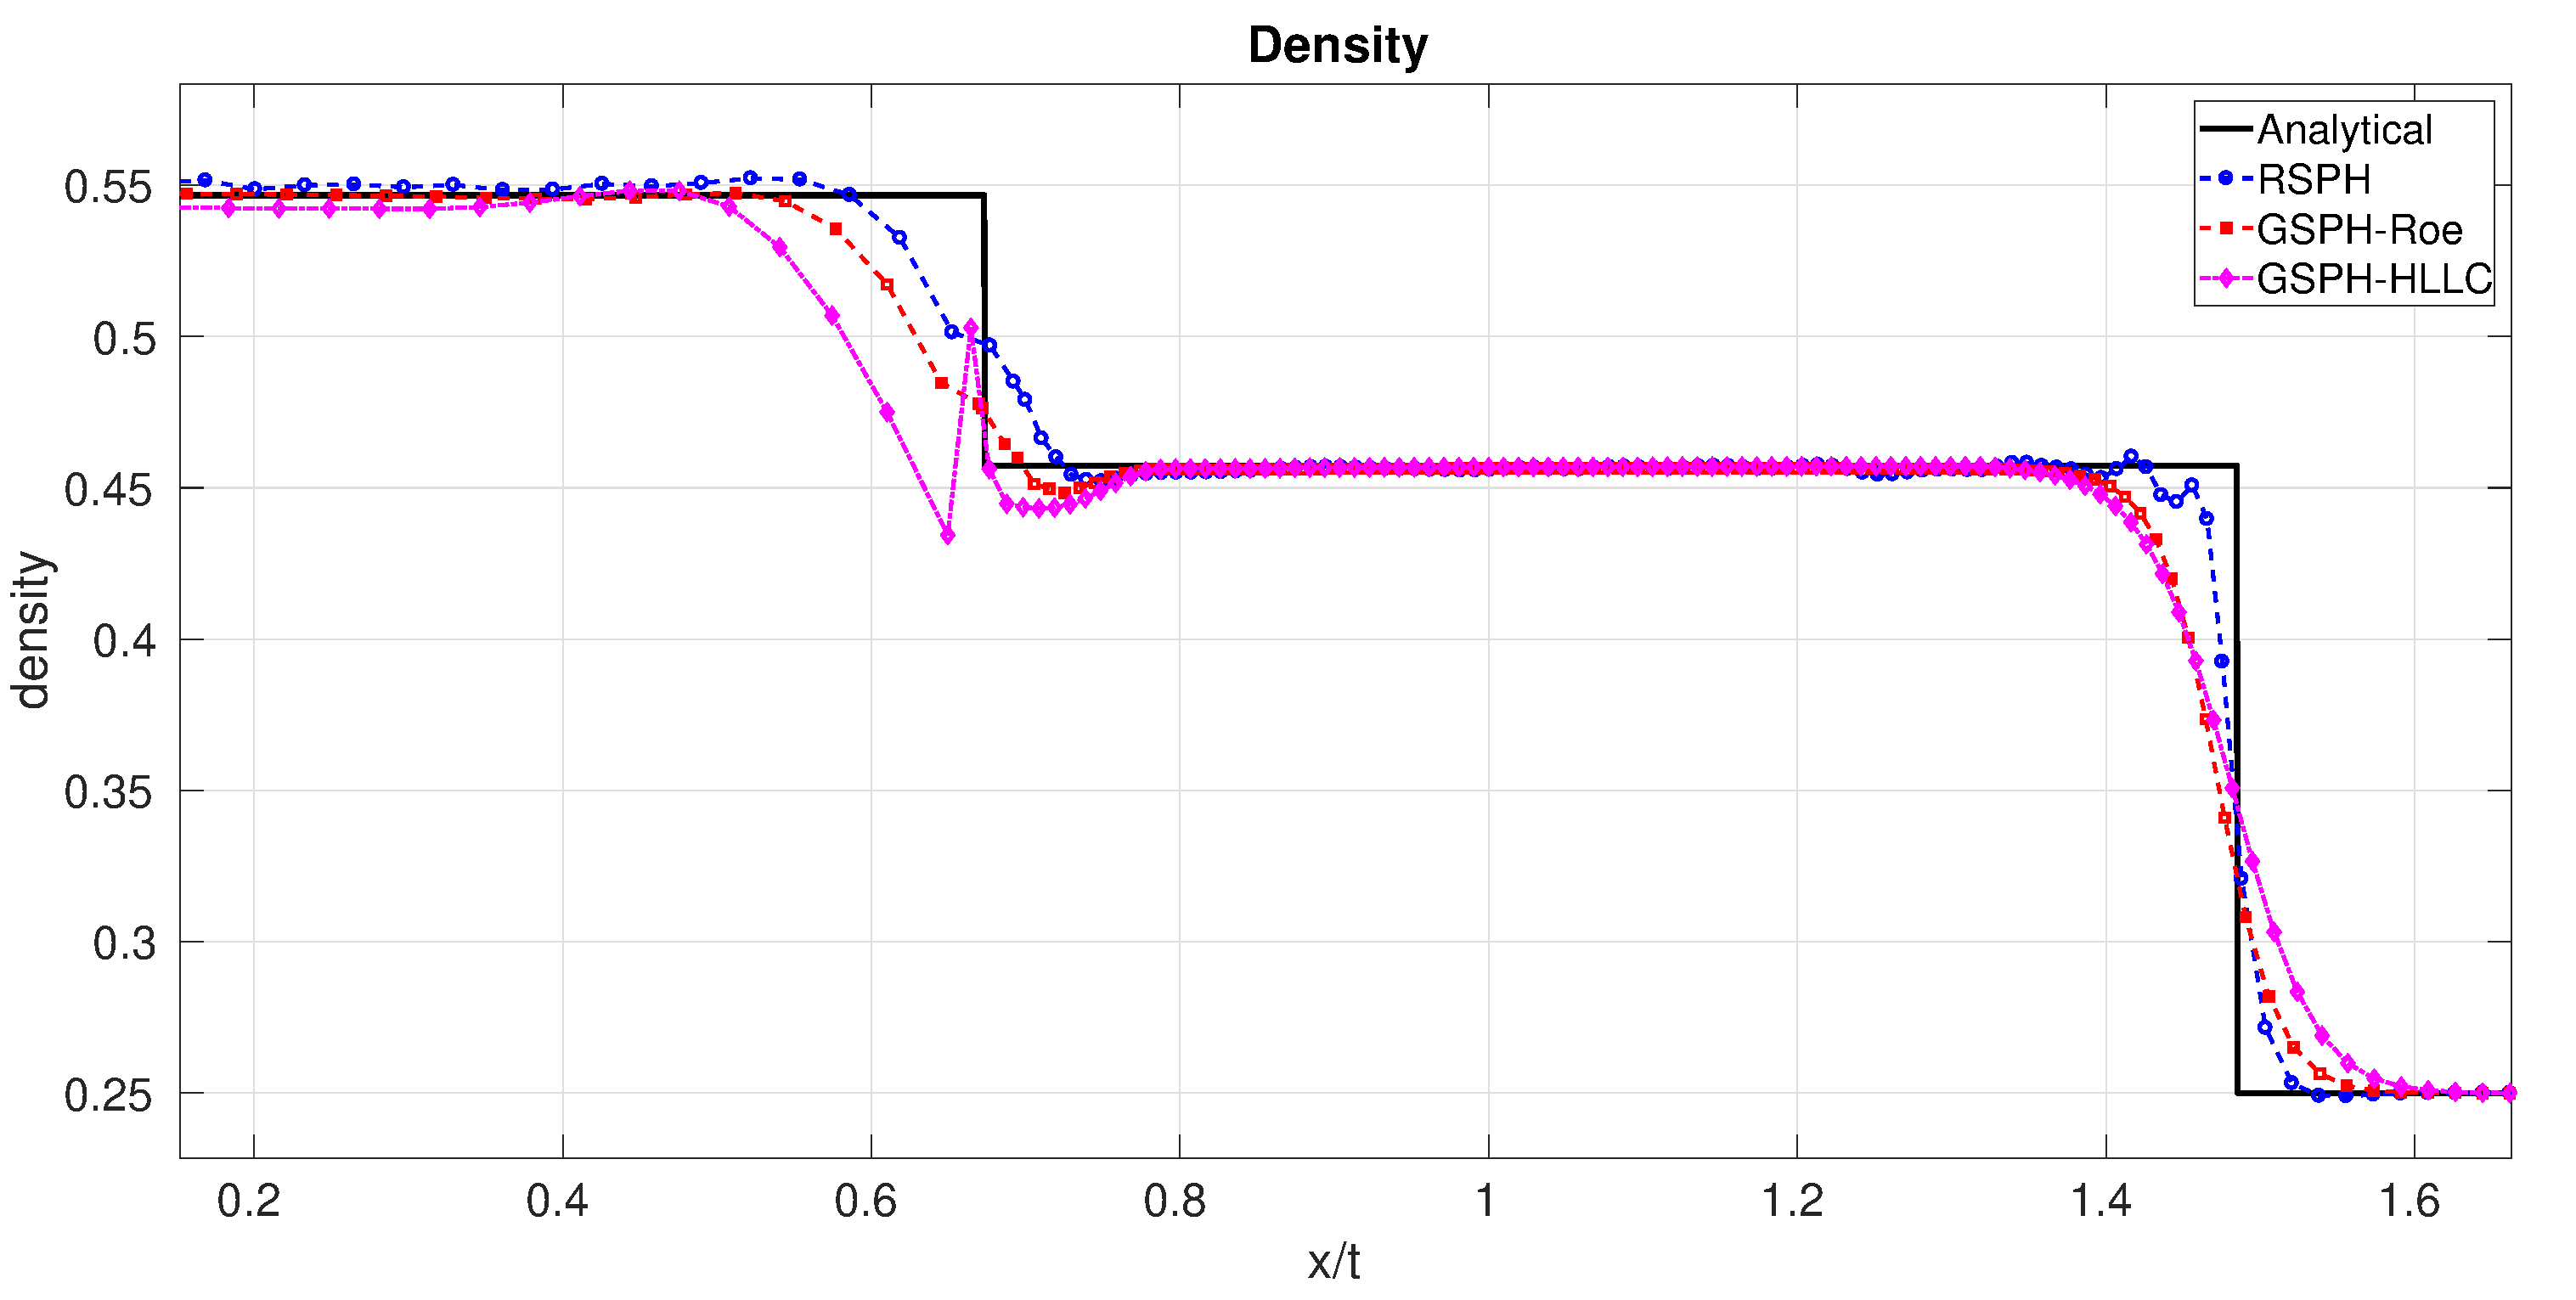
\includegraphics[width=0.99 \textwidth]{Chapter-4/Figures/Sod/RCM-Sod-GSPH-compare-rho-zoom}
    \end{minipage}%
    \begin{minipage}{.495 \textwidth}
        \centering
        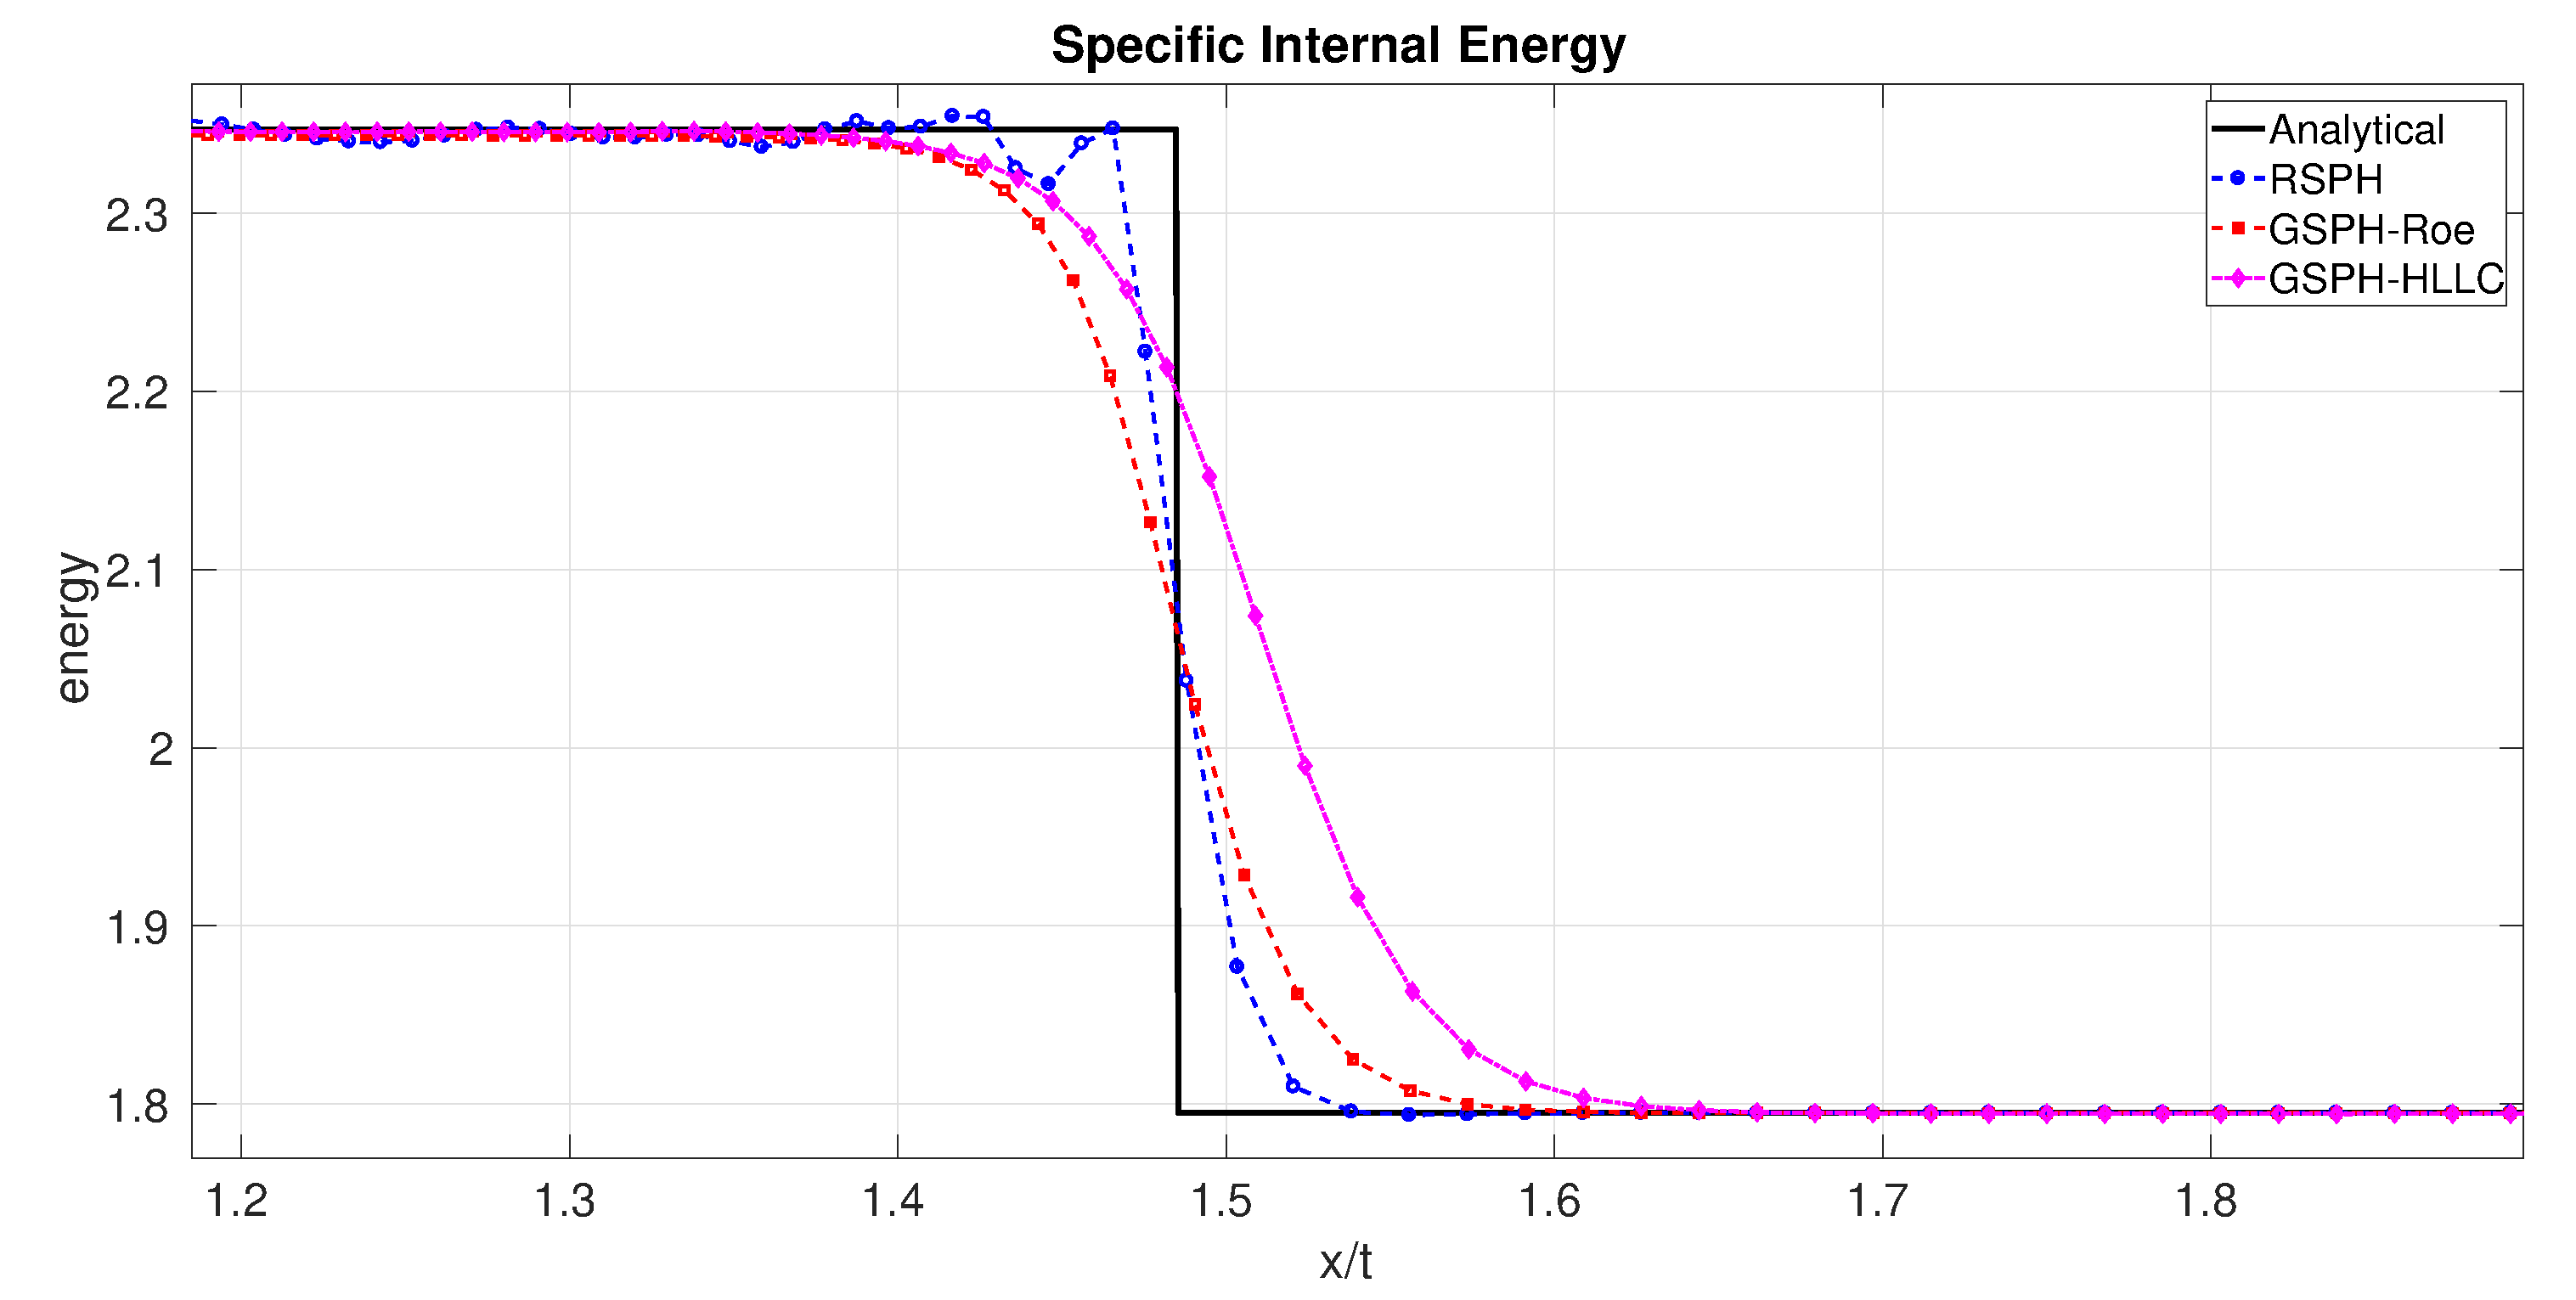
\includegraphics[width=0.99 \textwidth]{Chapter-4/Figures/Sod/RCM-Sod-GSPH-compare-e-zoom}
    \end{minipage}% 
    \\
    \begin{minipage}{.495 \textwidth}
        \centering
        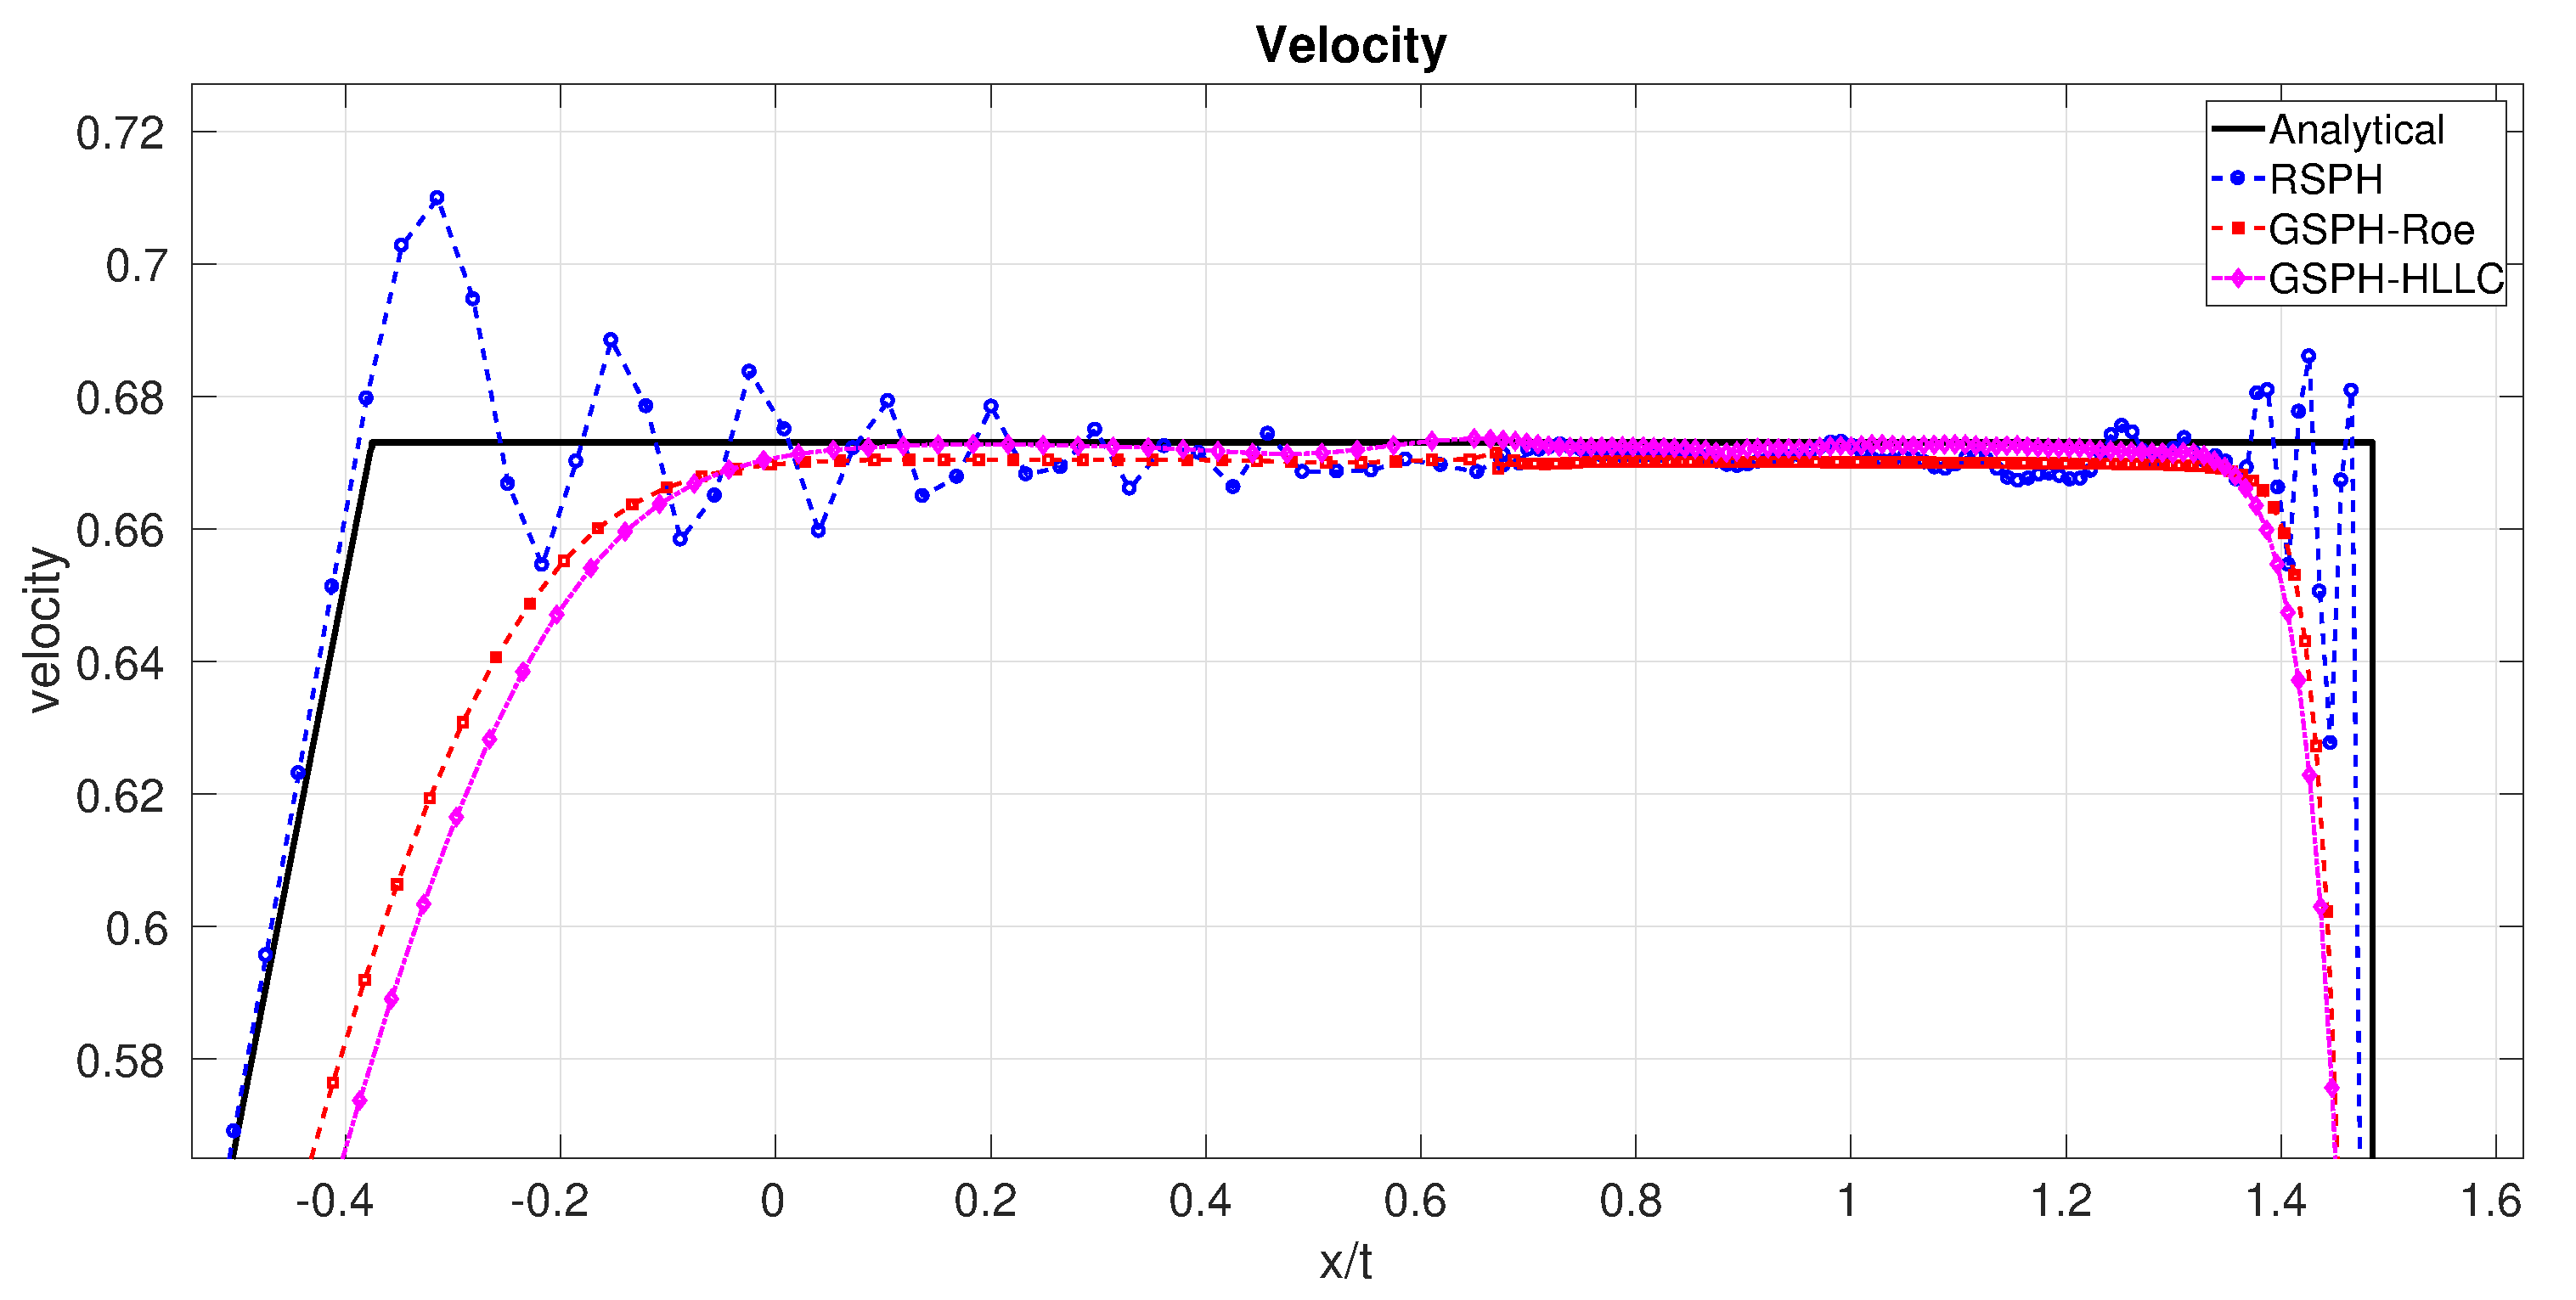
\includegraphics[width=0.99 \textwidth]{Chapter-4/Figures/Sod/RCM-Sod-GSPH-compare-v-zoom}
    \end{minipage}% 
    \begin{minipage}{.495\textwidth}
        \centering
        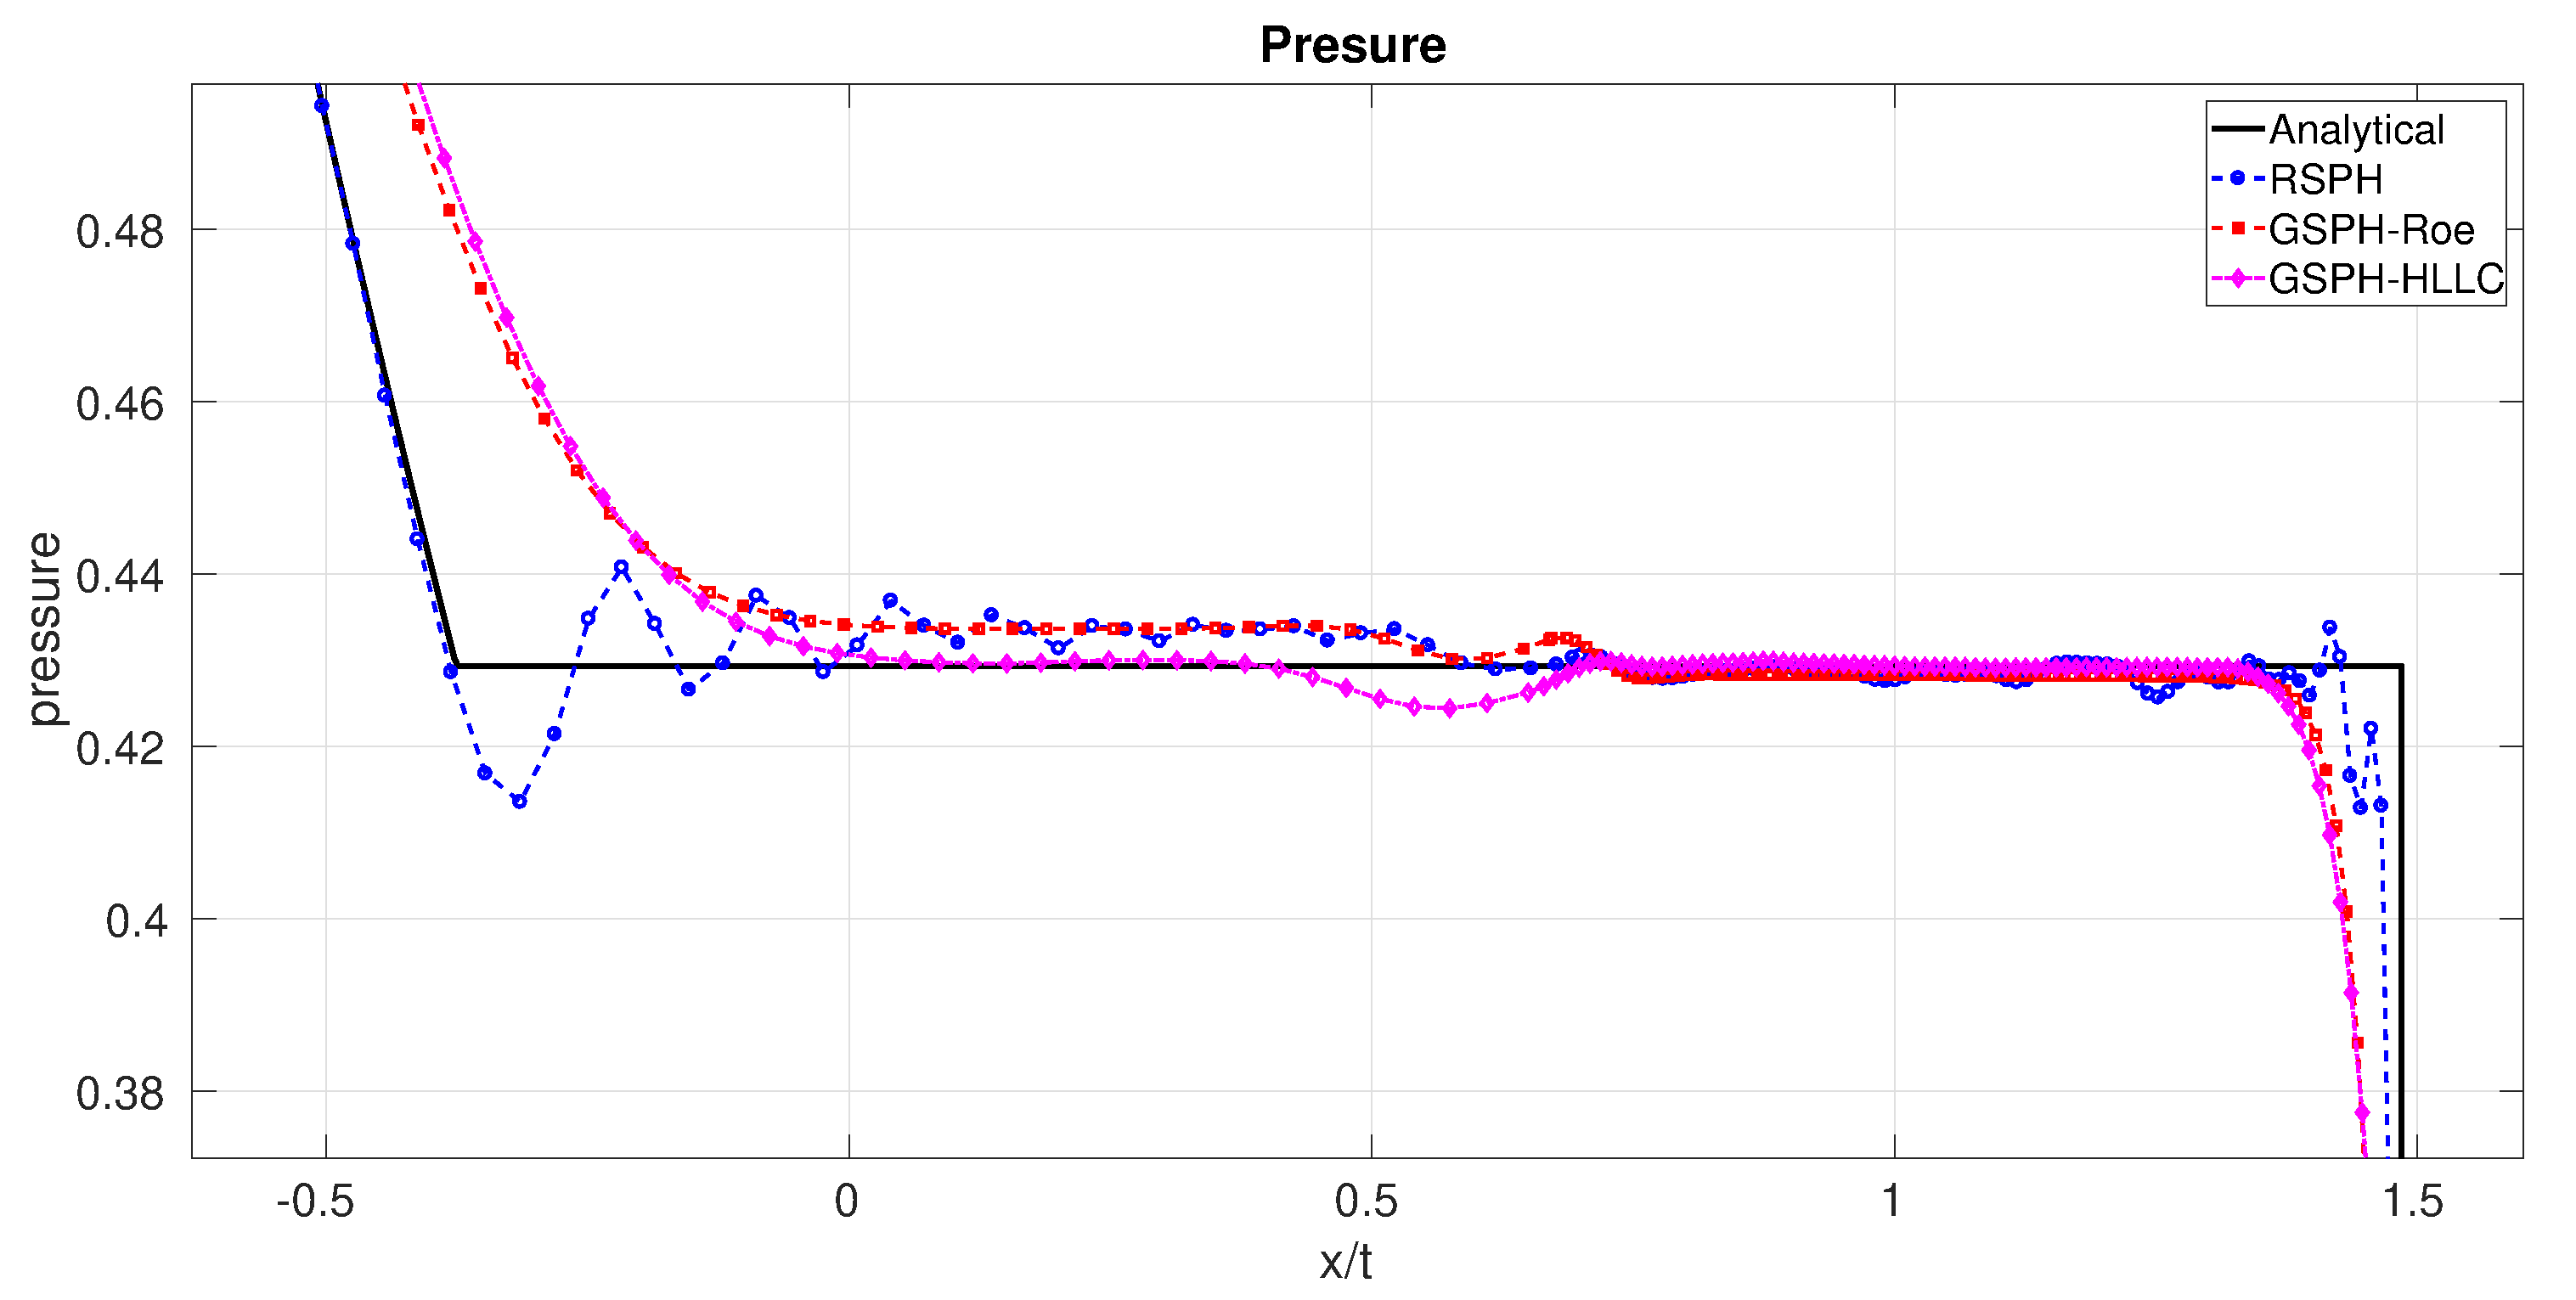
\includegraphics[width=0.99 \textwidth]{Chapter-4/Figures/Sod/RCM-Sod-GSPH-compare-p-zoom}
    \end{minipage}%    
    \caption{Comparison of RSPH with GSPH using Roe Riemann solver and HLLC Riemann solver. The last four plots are zoomed views. Zoomed view of density and specific internal energy show that GSPH smears the discontinuity at shock much more than RSPH. Zoomed view of velocity shows that fluctuation in GSPH is completely suppressed, which implies that numerical dissipation introduced in GSPH is at least around the same amount as SPH with $\alpha=1.0$. This is consistent with information implied by zoomed view of density and specific internal energy. The last zoomed view shows that both RSPH and GSPH can get rid of pressure ``wiggle" around the contact discontinuity.}
    \label{fig:RCM-Sod-GSPH}
\end{figure}

These zoomed views in fig. \ref{fig:RCM-Sod-GSPH} demonstrate that RSPH introduces less but sufficient dissipation compared with GSPH. The attractive feature of RCM method in preserving true discontinuity is inherited by RSPH in this 1D shock tube test. With more dissipation, GSPH can completely suppress numerical dissipation. The discontinuity at the shock is more seriously smeared. The excessive amount dissipation might have other, more undesirable, effects in real implementation. For example, over damping of shearing flow. Compared with SPH, both GSPH and RSPH avoid pressure ``wiggle" around contact discontinuity. Since RSPH share many common places with Godunov's method, it is not surprise that RSPH can also suppress the pressure ``wiggle" at contact discontinuity.

\subsection{Accuracy tests}
We use shock tube test to gauge the accuracy of the RSPH scheme.
% for both situations when the solution remains smooth and when there are shocks in the solution. We use test 1 to conduct order of accuracy test for the case with shocks in the solution. 
We examine the errors between simulation results and the analytical solution (the reference solution) as the number of particles is increased. The $L_1$ norm error, defined for a property $f$, is normalized by the number of particles as:
\begin{equation}
L_1= \frac{1}{N_p} \sum_a^{N_p} \vert f_a^{SPH} - f^{REF} (x_a) \vert 
\end{equation}
where the superscript $REF$ represent the reference solution, $SPH$ represents simulation results calculated by different SPH schemes. Fig. \ref{fig:Accuracy-test1} displays the $L_1$ norm errors for the density, velocity and pressure profiles for different SPH schemes.
We observe a rate of convergence of approximately 1 for GSPH and 1.5 for standard SPH and RSPH.
GSPH with an exact Riemann solver has been shown to be approximately second order of accuracy \citep{puri2014comparison} and comparable in accuracy to the standard SPH schemes when using piece wise linear construction. As for GSPH using approximate Riemann solver, \citet{puri2014approximate} reported second order accuracy for HLLC and Roe Riemann solvers adopting piece wise linear Riemann problem construction. In addition, they adopted a test problem without discontinuity in the solution. Existing of discontinuities, such as shock, in the test problem might lower rate of convergence. Both RSPH and GSPH tests in this paper adopt a piece wise constant construction of Riemann problem. So we conclude that RSPH shows higher order of accuracy than GSPH when using the same Riemann problem construction. Compared with SPH, RSPH shows almost the same order of accuracy and level of error.
%It is worthwhile to check the order of accuracy of GSPH using piecewise linear constructor
%It is also worthwile to check what of order of accuracy using another test problem.  
\begin{figure}[H]
    \centering
    \begin{minipage}{.332\textwidth}
        \centering
        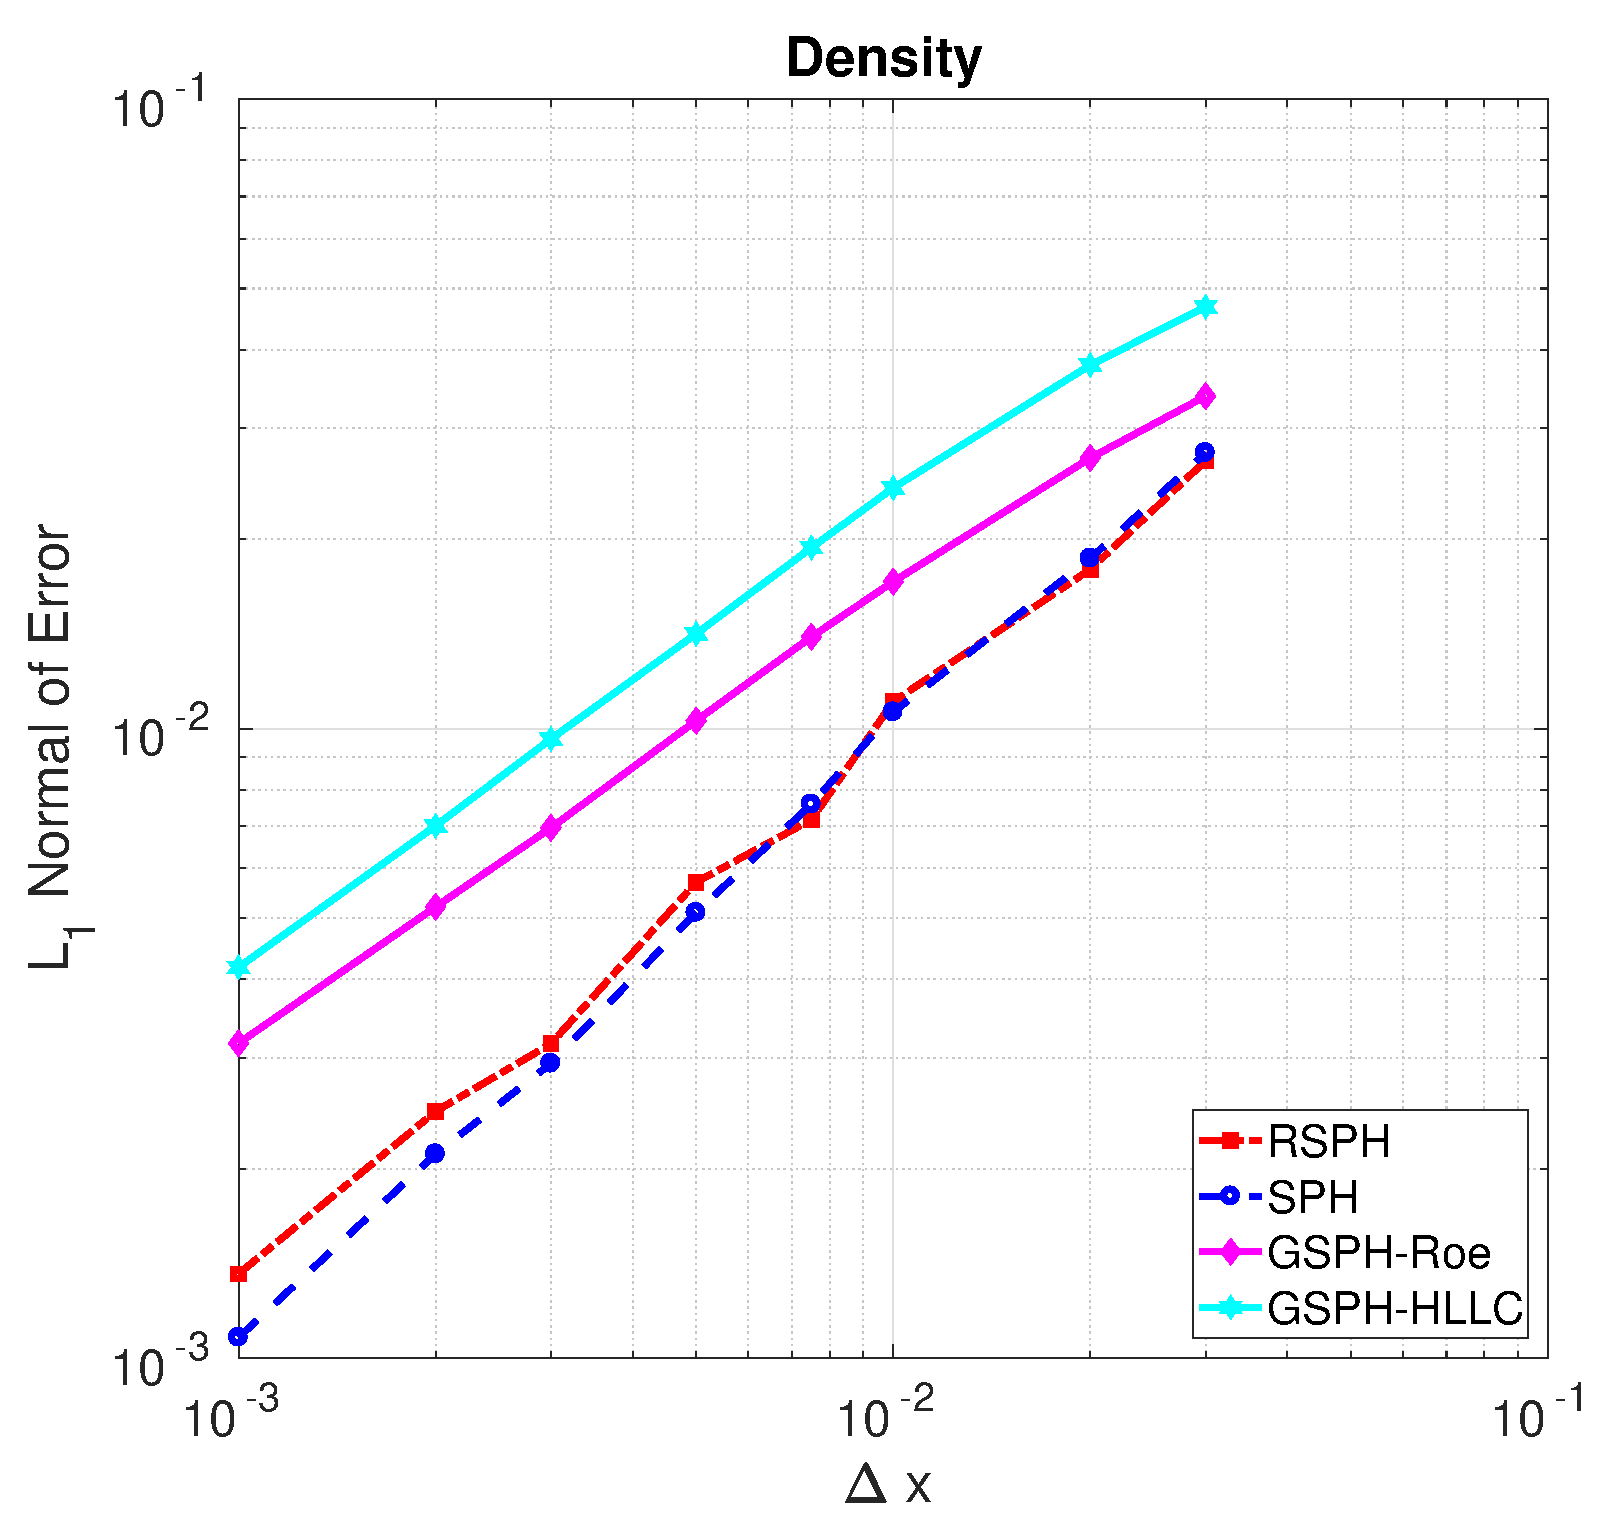
\includegraphics[width=0.99 \textwidth]{Chapter-4/Figures/Accuracy-des}
    \end{minipage}%
    \begin{minipage}{.332 \textwidth}
        \centering
        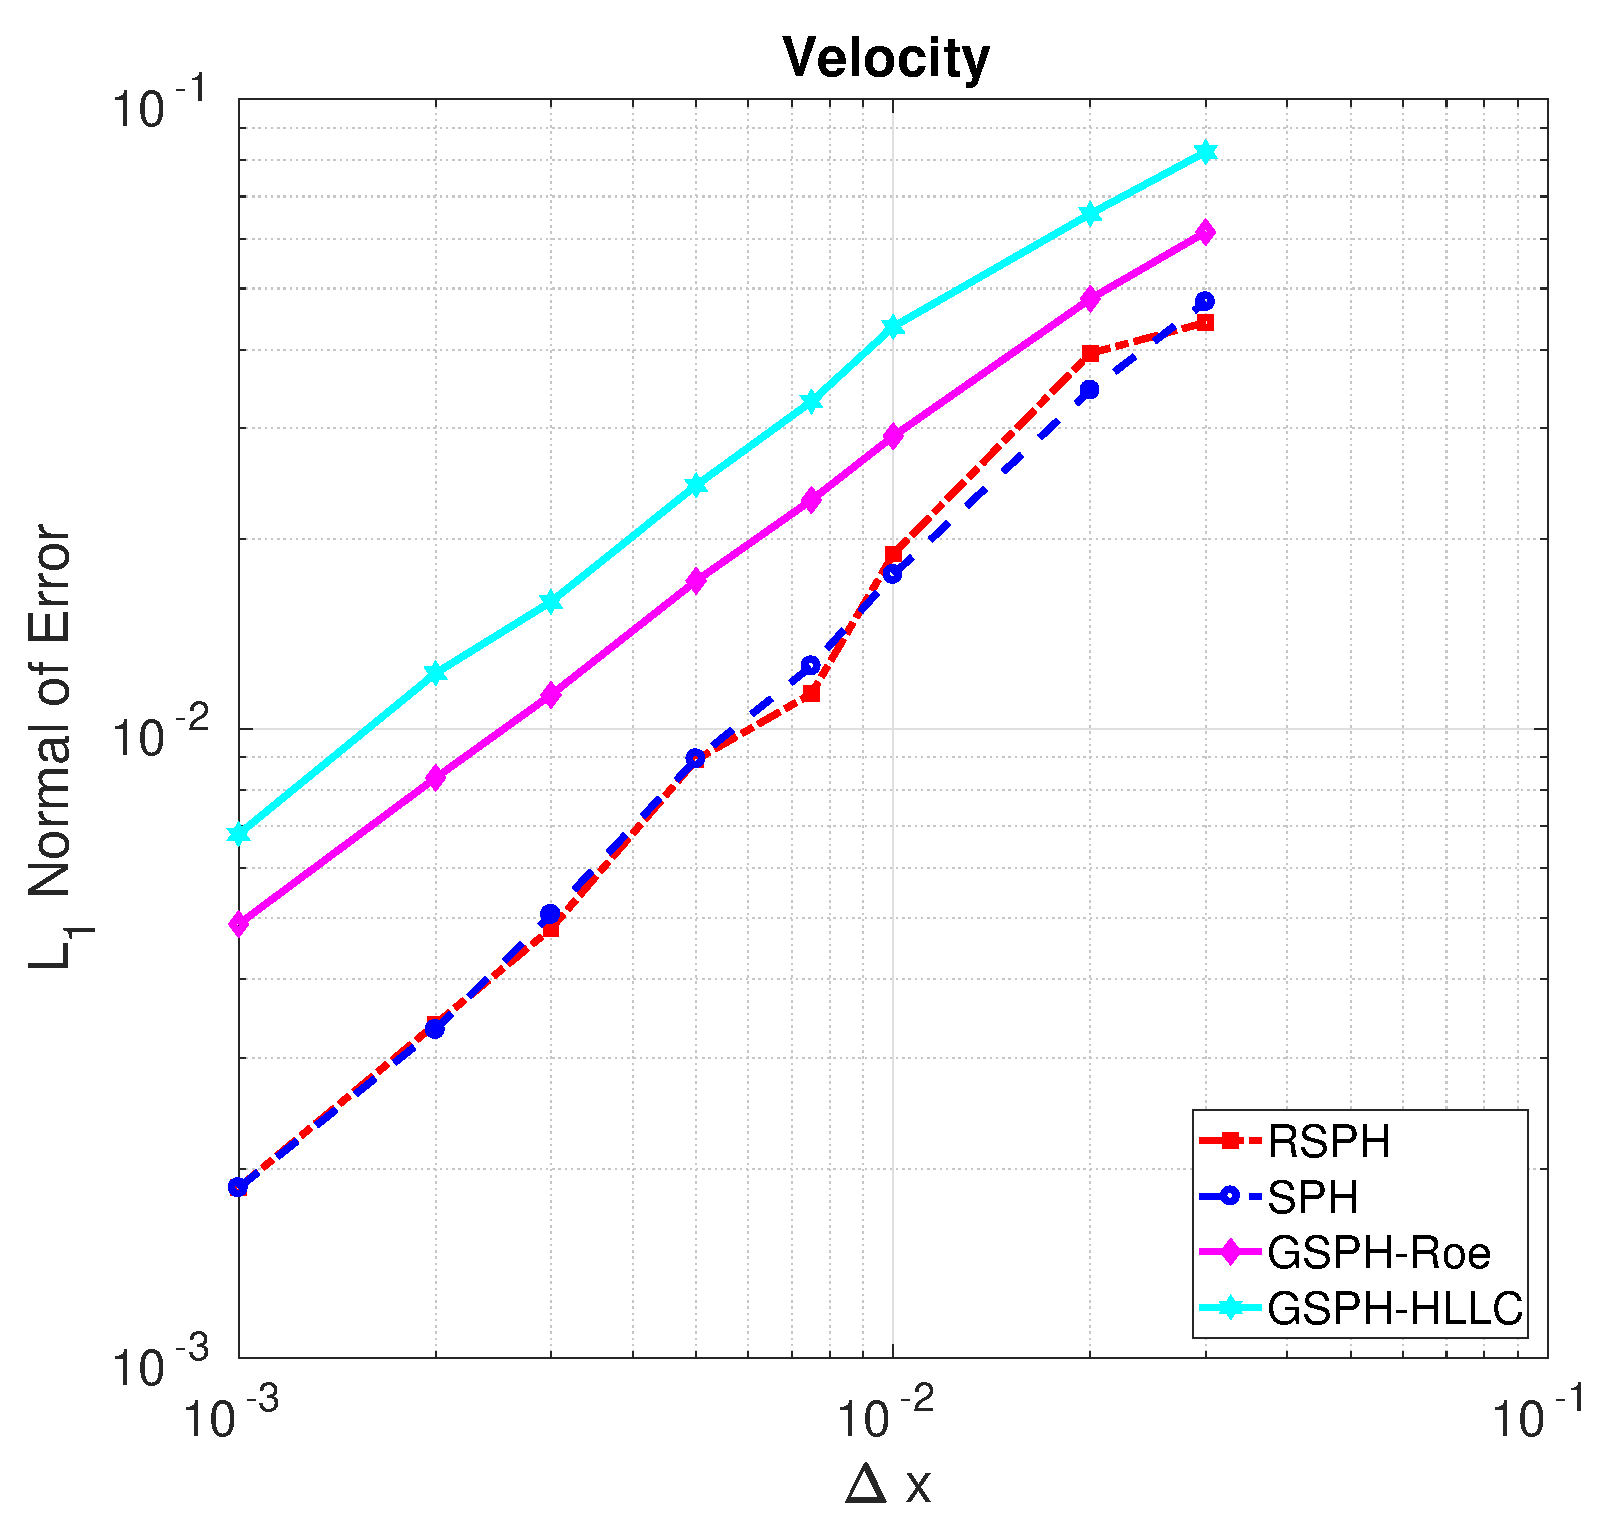
\includegraphics[width=0.99 \textwidth]{Chapter-4/Figures/Accuracy-vel}
    \end{minipage}%
    \begin{minipage}{.332\textwidth}
        \centering
        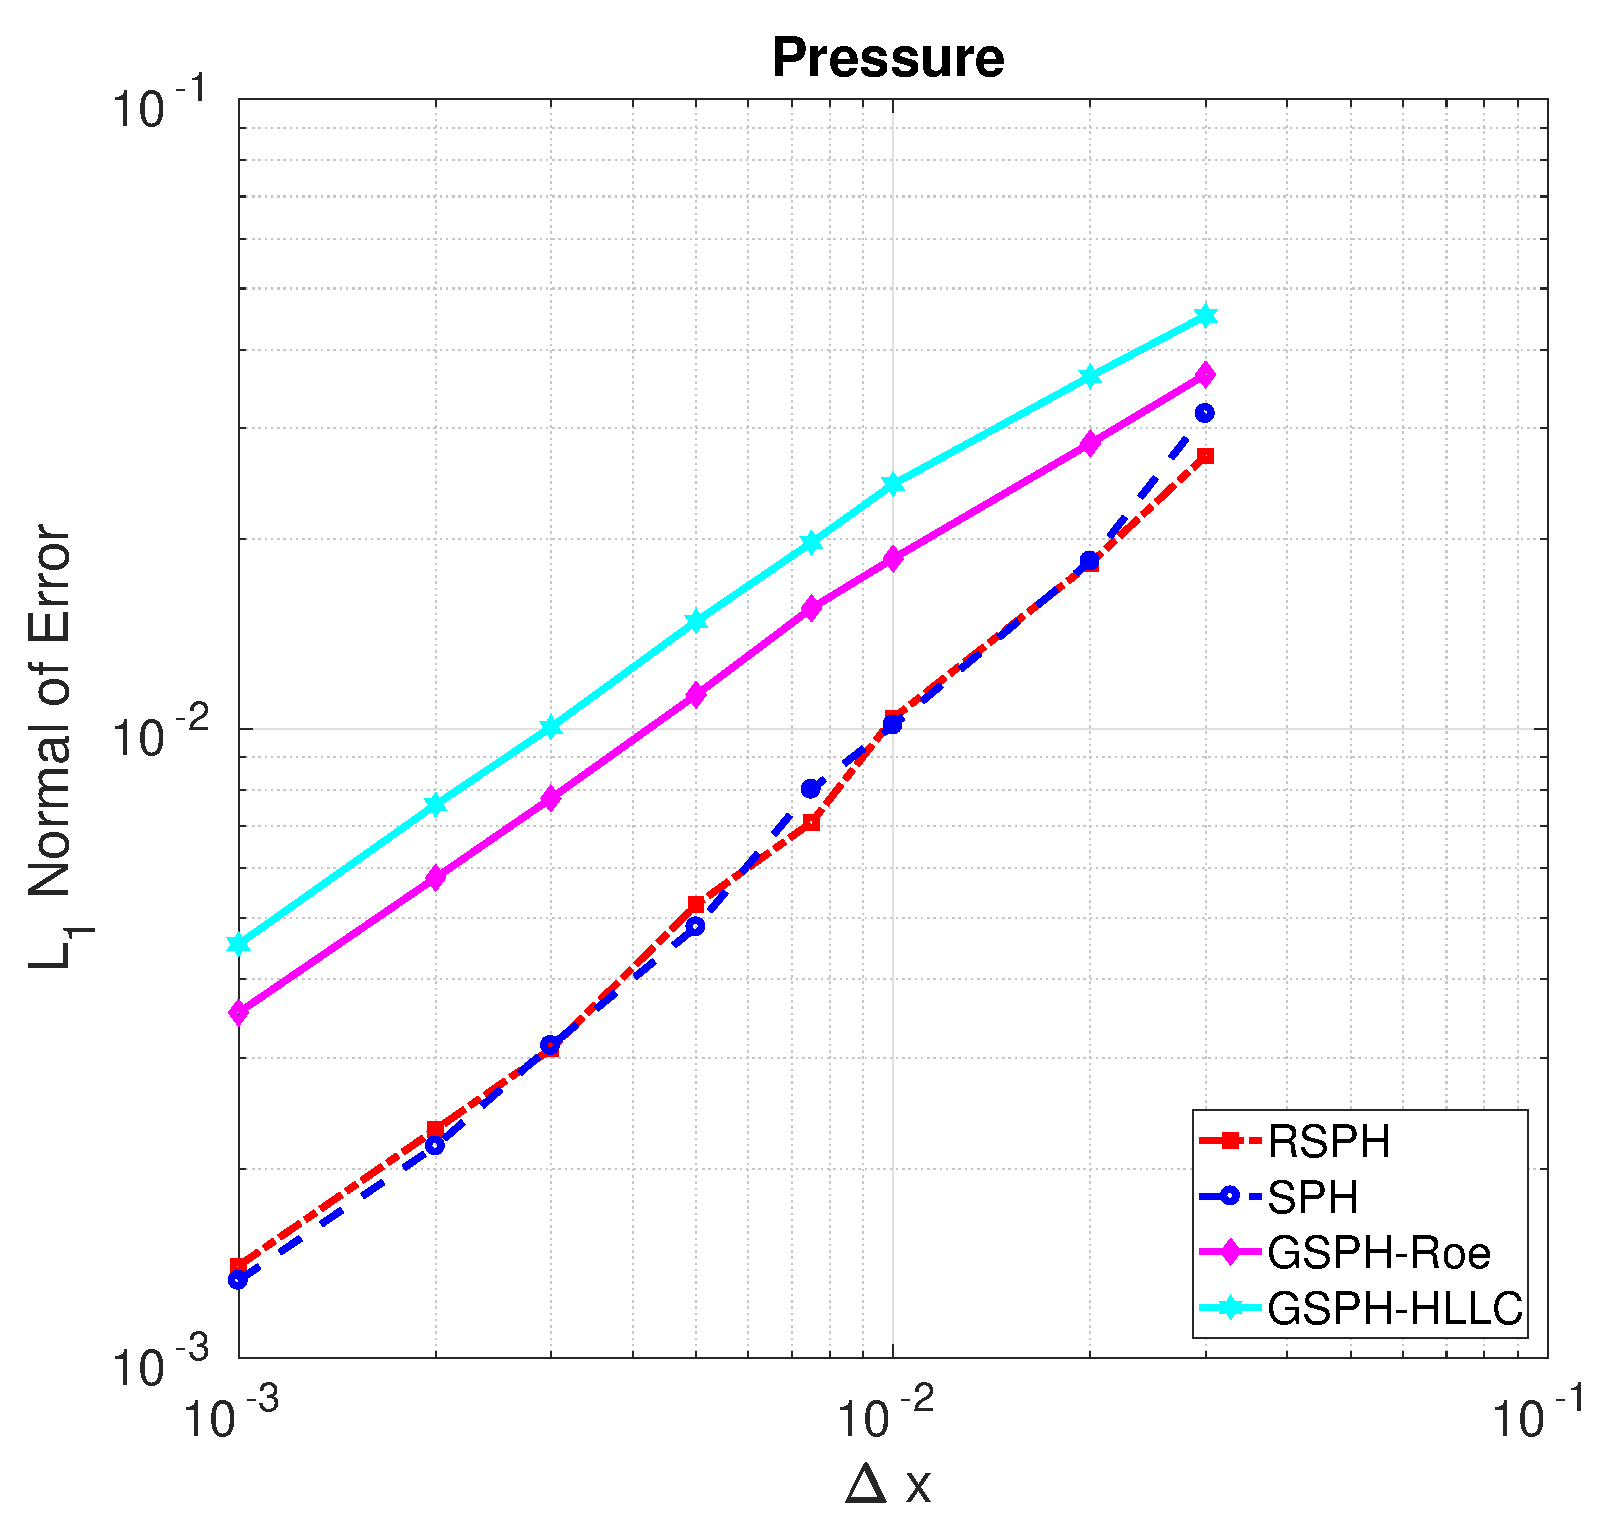
\includegraphics[width=0.99 \textwidth]{Chapter-4/Figures/Accuracy-pre}
    \end{minipage}%  
    \caption{ $L_1$ norm errors for 1D shock tube test (test1) for RSPH, standard SPH, GSPH using Roe Riemann solver and GSPH using HLLC Riemann Solver.  GSPH with the HLLC approximate Riemann solver exhibits the same convergence rate (around 1) but quantitatively larger errors than that with Roe Riemann solver. RSPH and standard SPH shows same rate of convergence and almost same amount of error.}
    \label{fig:Accuracy-test1}
\end{figure}
 
\subsection{Comprehensive 1D tests} \label{sec:comprehensive-1d-tests}
Comprehensive tests are presented in this section to check how well does RSPH work for different situations. Input parameters for each tests is given in Table \ref{tab:1D-shock-input_parameters}. Wave speed is estimated based on formulation Eq. (\ref{eq:RP-solver-HLLC-SM}) $\sim$ Eq. (\ref{eq:RP-solver-HLLC-SR}).
The results are shown in Fig. \ref{fig:RCM-GSPH-Sod} $\sim$ Fig. \ref{fig:RCM-strong-blast}. $x$ axis in these plots are normalized by the terminal time $t_f$. We observe that RSPH is able to correctly predict the position and magnitude of all waves for all tests. A jump of specific internal energy at the origin is observed in Sjogreen test. However, such jump is a common issue of SPH schemes and has been reported in many other tests (see, for example, \citep{monaghan1997sph,cha2003implementations,puri2014approximate})
In addition, a noticeable spike can be observed near the contact discontinuity. Similar spike is observed in GSPH simulation \citep{puri2014comparison}. Such spike is evident in the FVM solution as well and is perhaps an artifice of the Lagrangian nature of the two schemes. \citep{noh1987errors} proposed to adding a small amount of thermal conduction to ameliorate the spike and has been applied in blast-wave test using GSPH \citep{puri2014comparison}. We did not adopt such strategy in our simulation.
Due to less amount of dissipation, numerical fluctuations persist in all simulation results. For the strong blast test and double shock test, such fluctuations become more obvious than other tests. Even though, the magnitude of fluctuations is within acceptable range.

\begin{figure}[H]
    \centering
    \begin{minipage}{.495\textwidth}
        \centering
        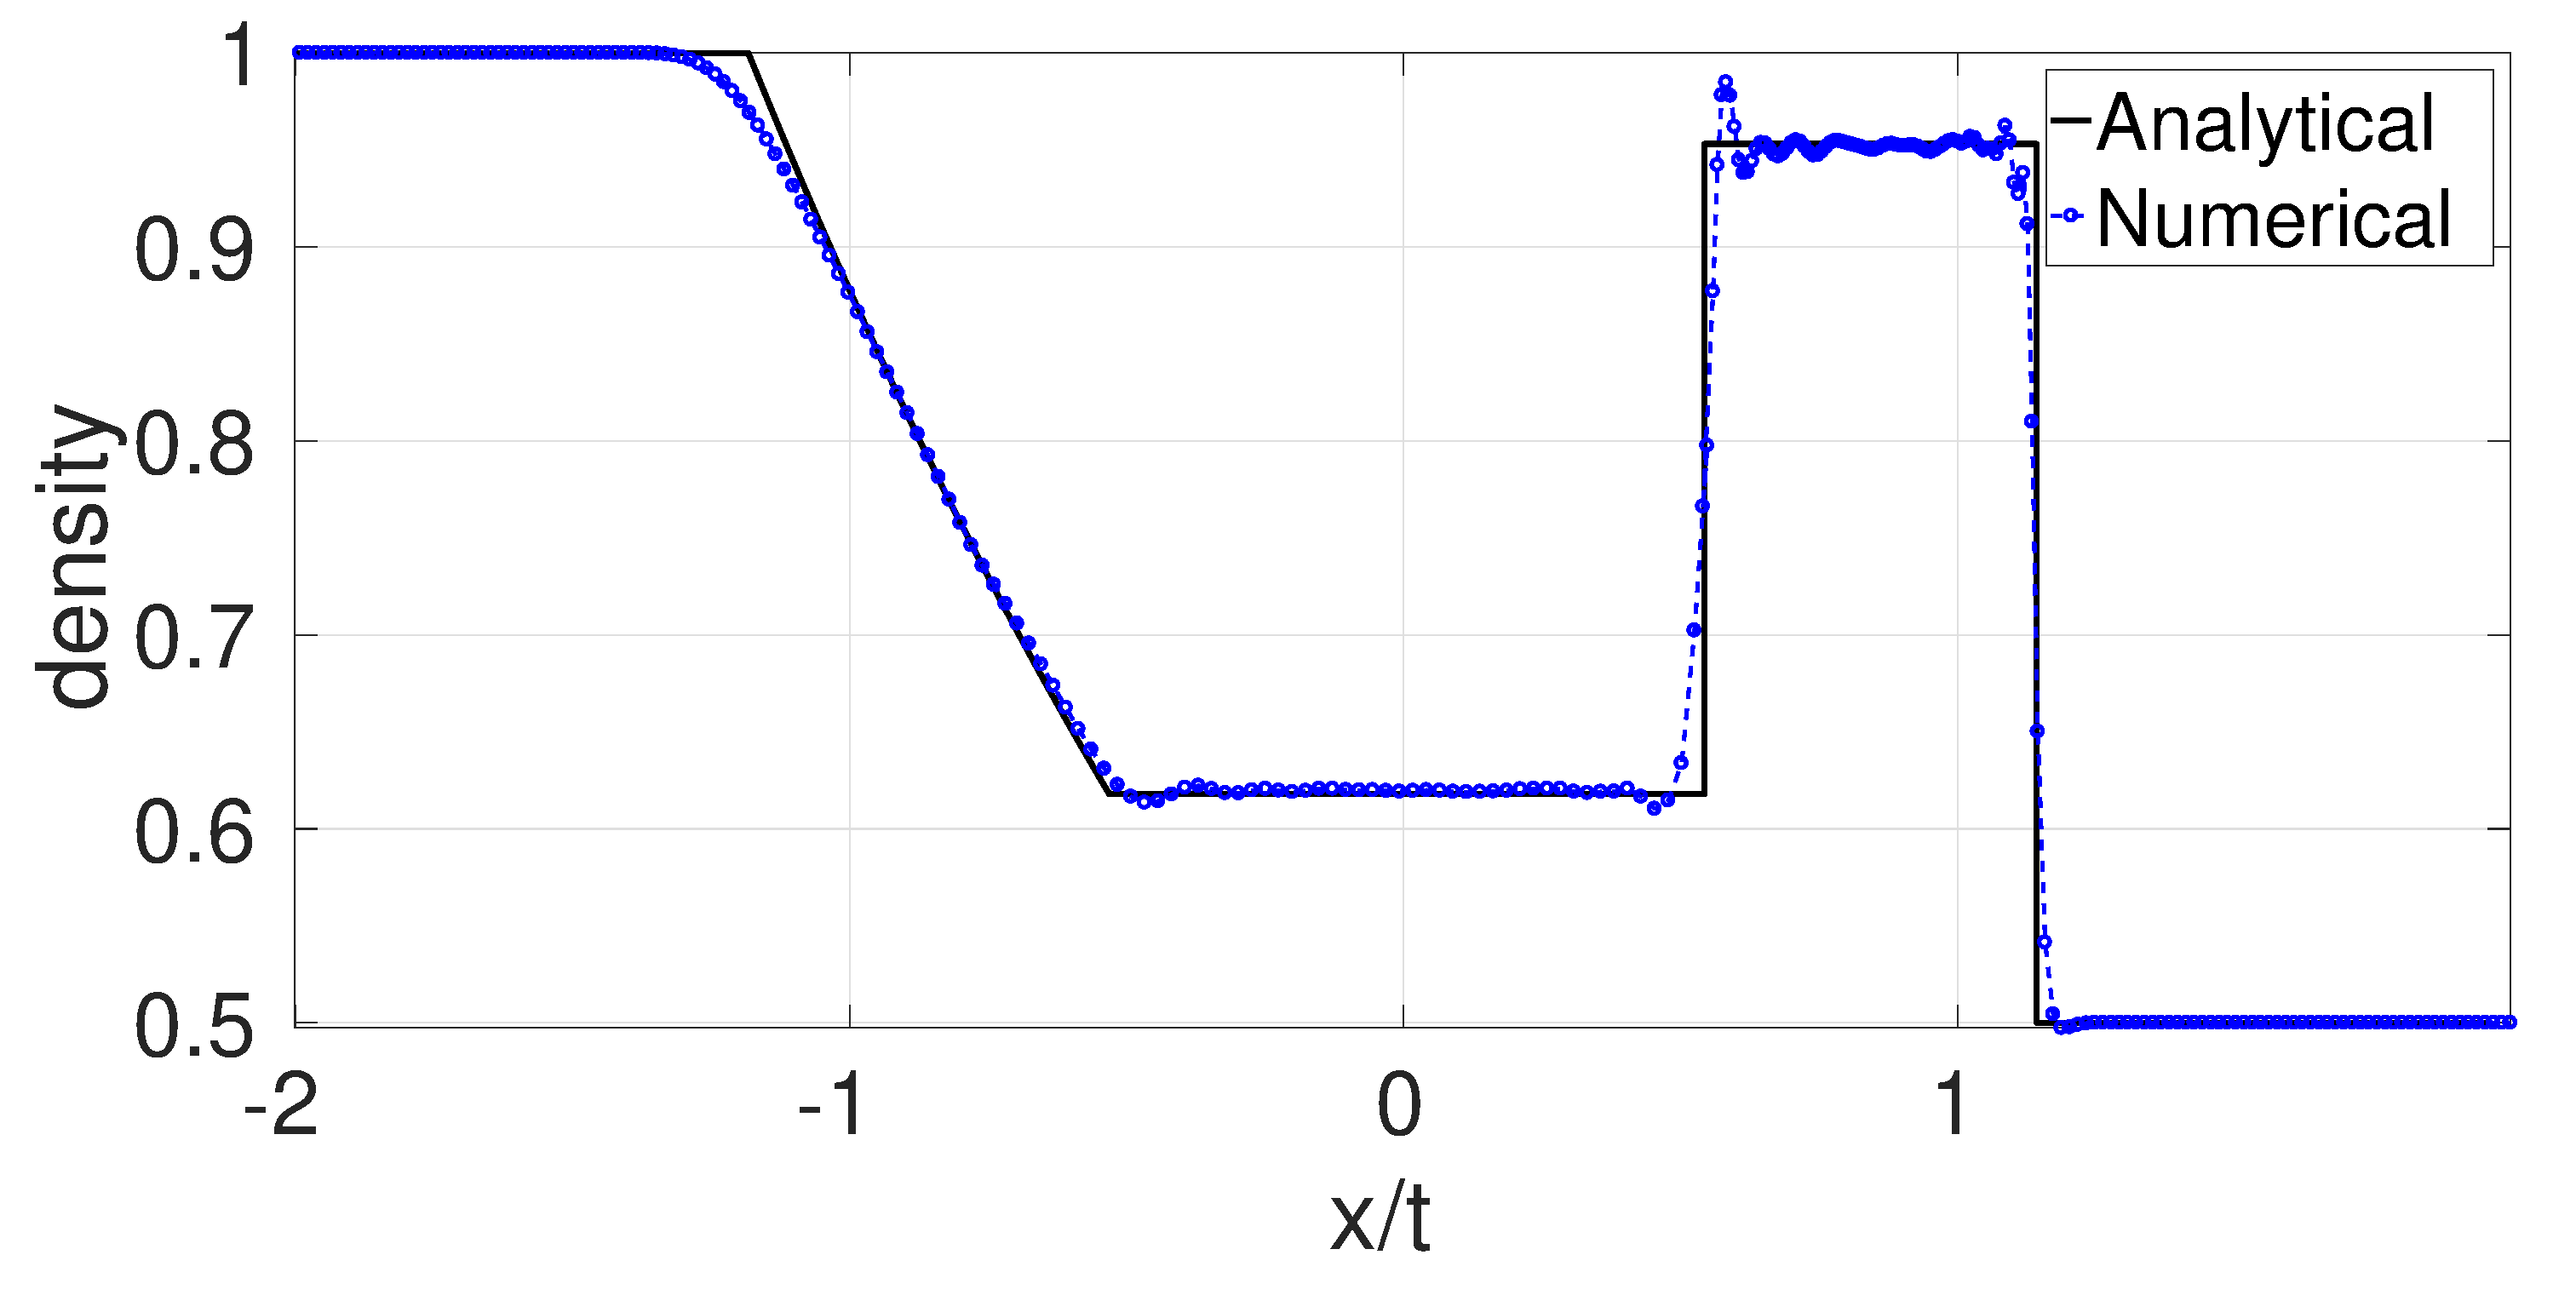
\includegraphics[width=0.99 \textwidth]{Chapter-4/Figures/GSPH-Sod/GRod-RCM-rho}
    \end{minipage}%
    \begin{minipage}{.495 \textwidth}
        \centering
        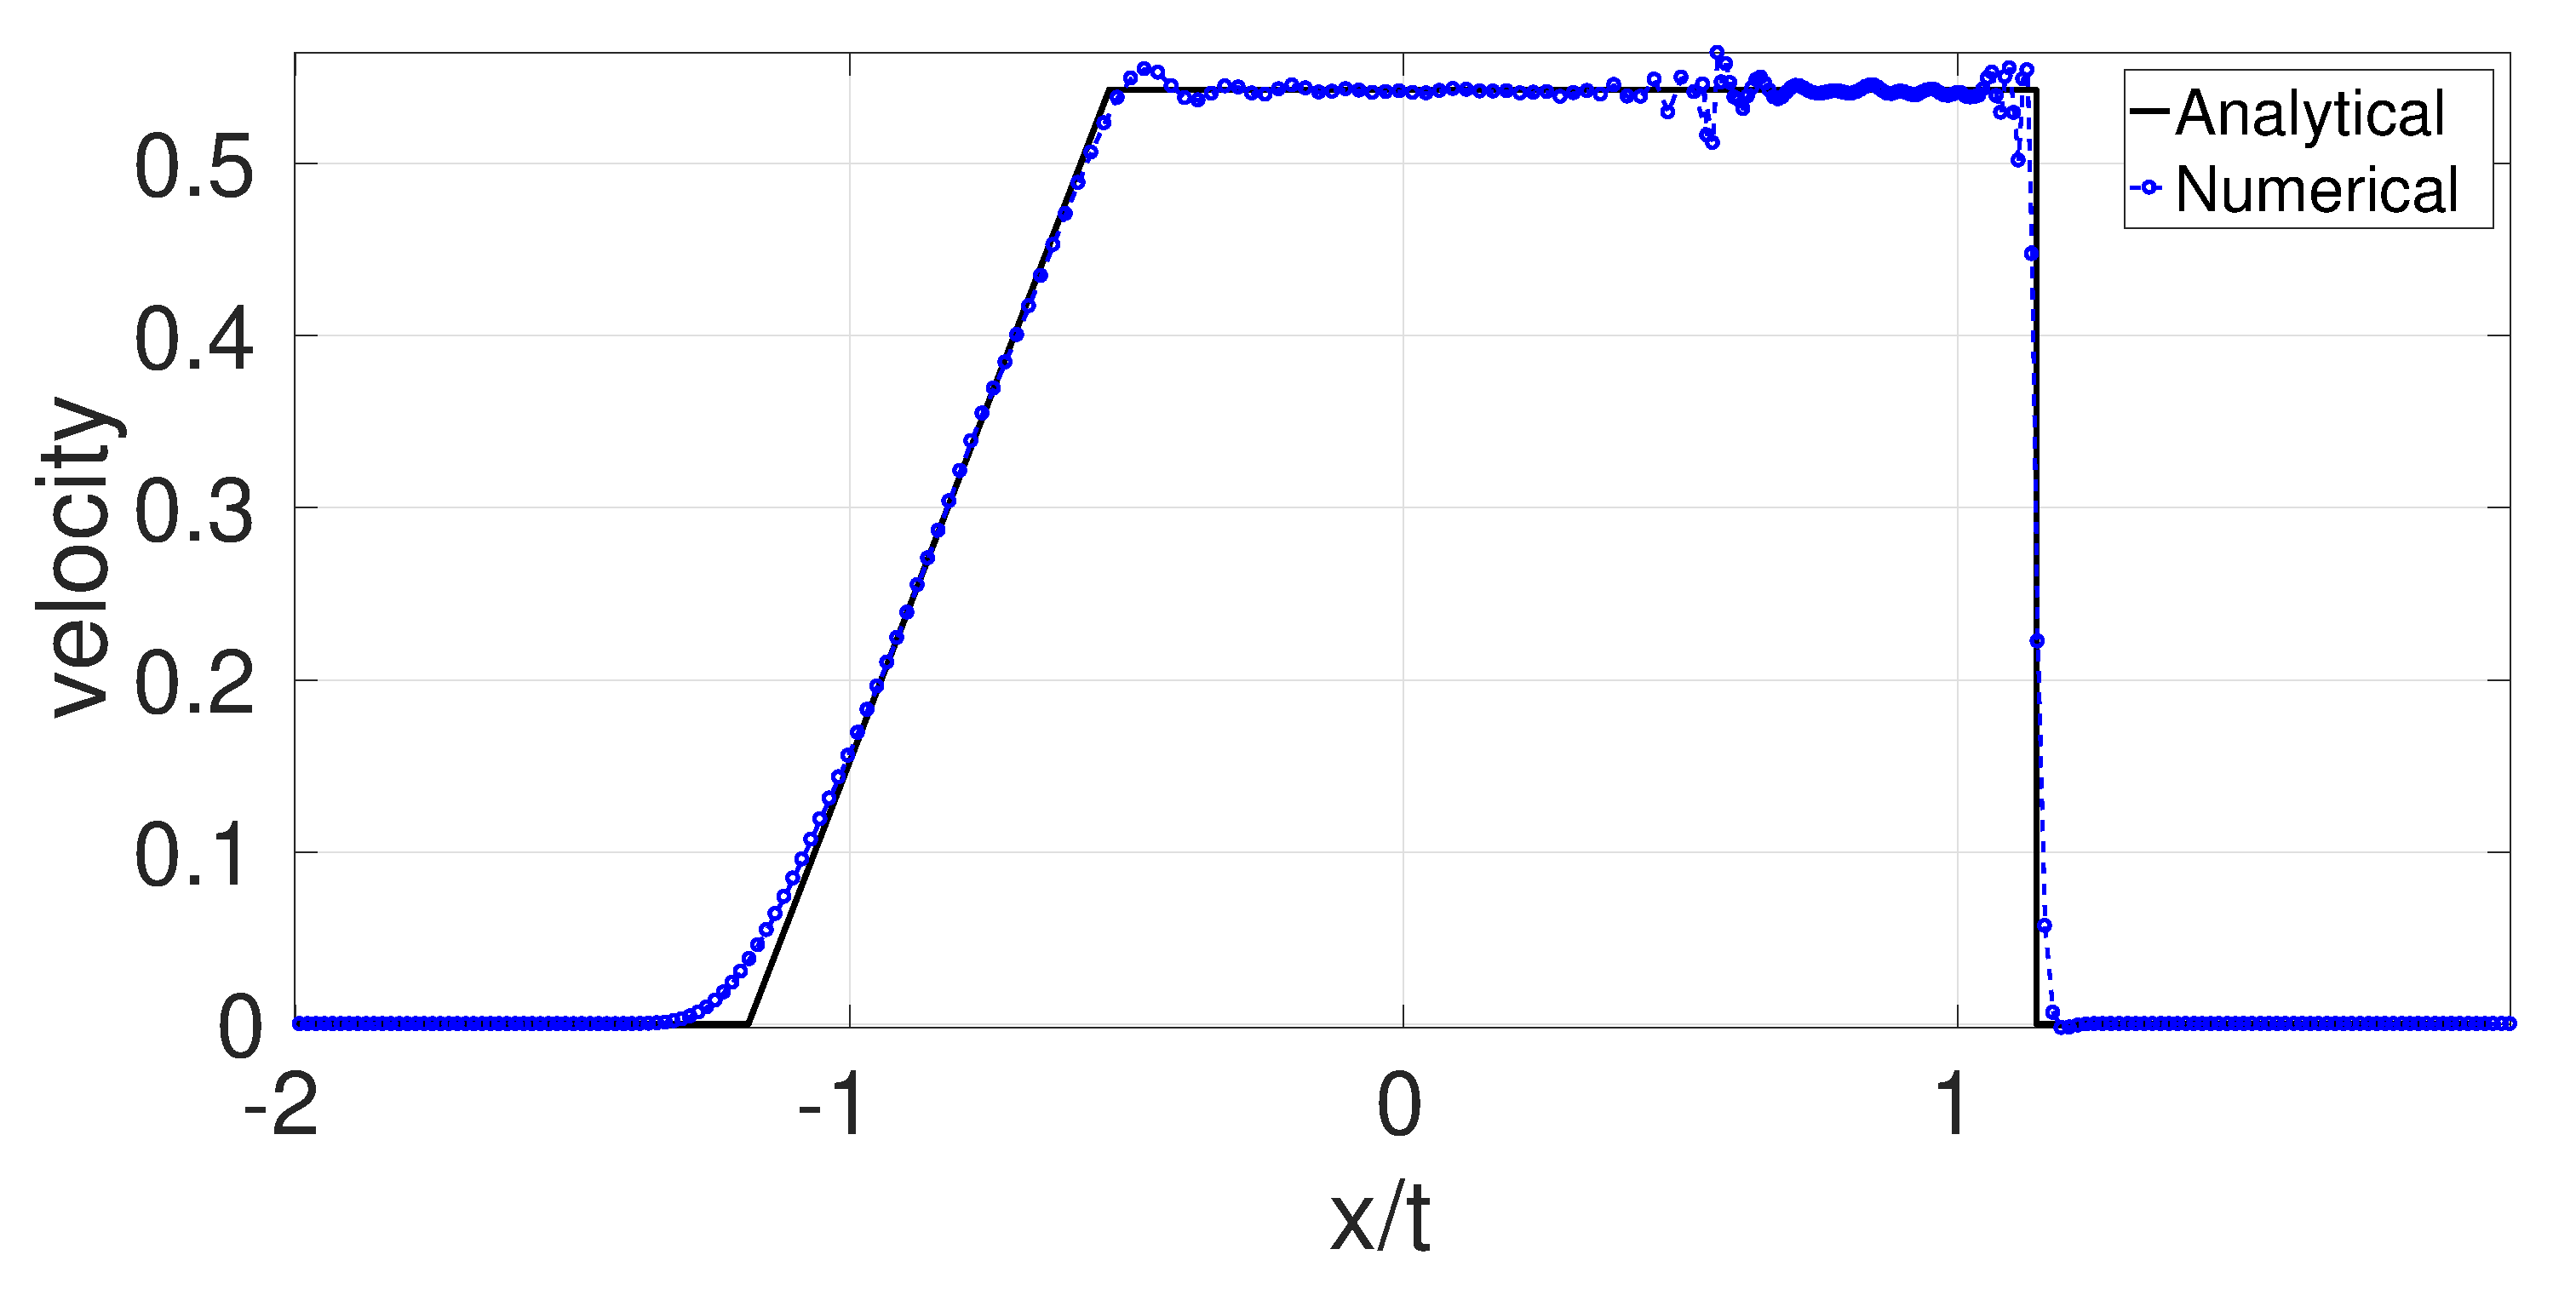
\includegraphics[width=0.99 \textwidth]{Chapter-4/Figures/GSPH-Sod/GRod-RCM-v}
    \end{minipage}% 
    \\
    \begin{minipage}{.495\textwidth}
        \centering
        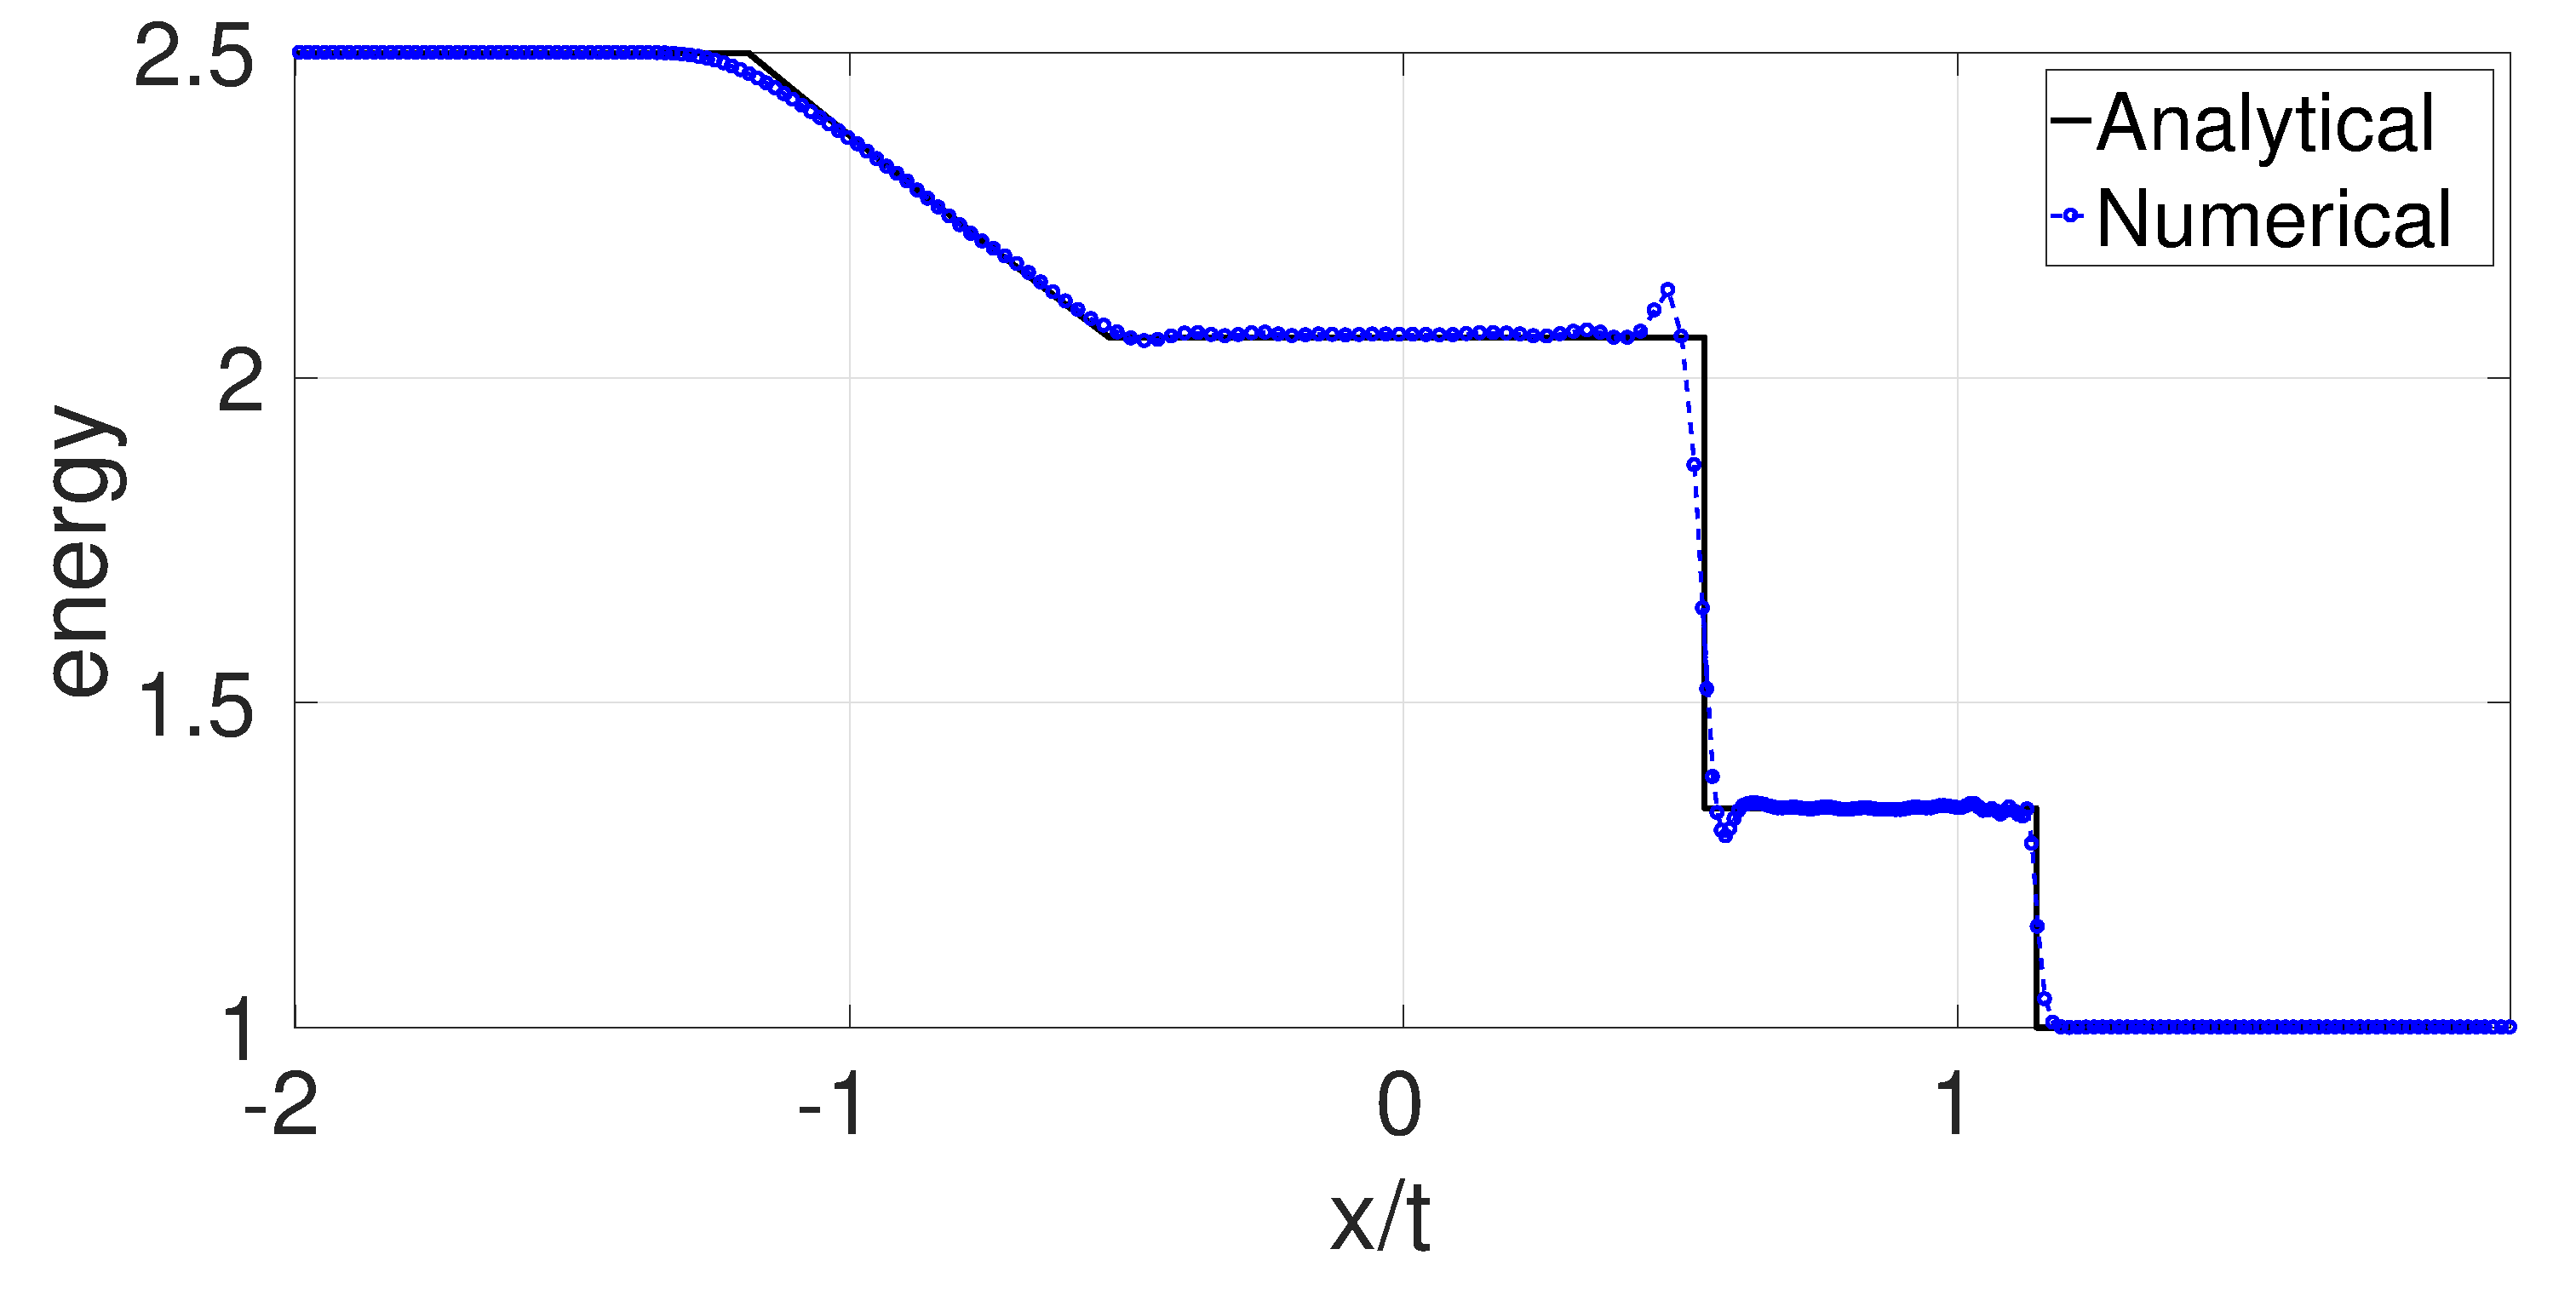
\includegraphics[width=0.99 \textwidth]{Chapter-4/Figures/GSPH-Sod/GRod-RCM-e}
    \end{minipage}%
    \begin{minipage}{.495 \textwidth}
        \centering
        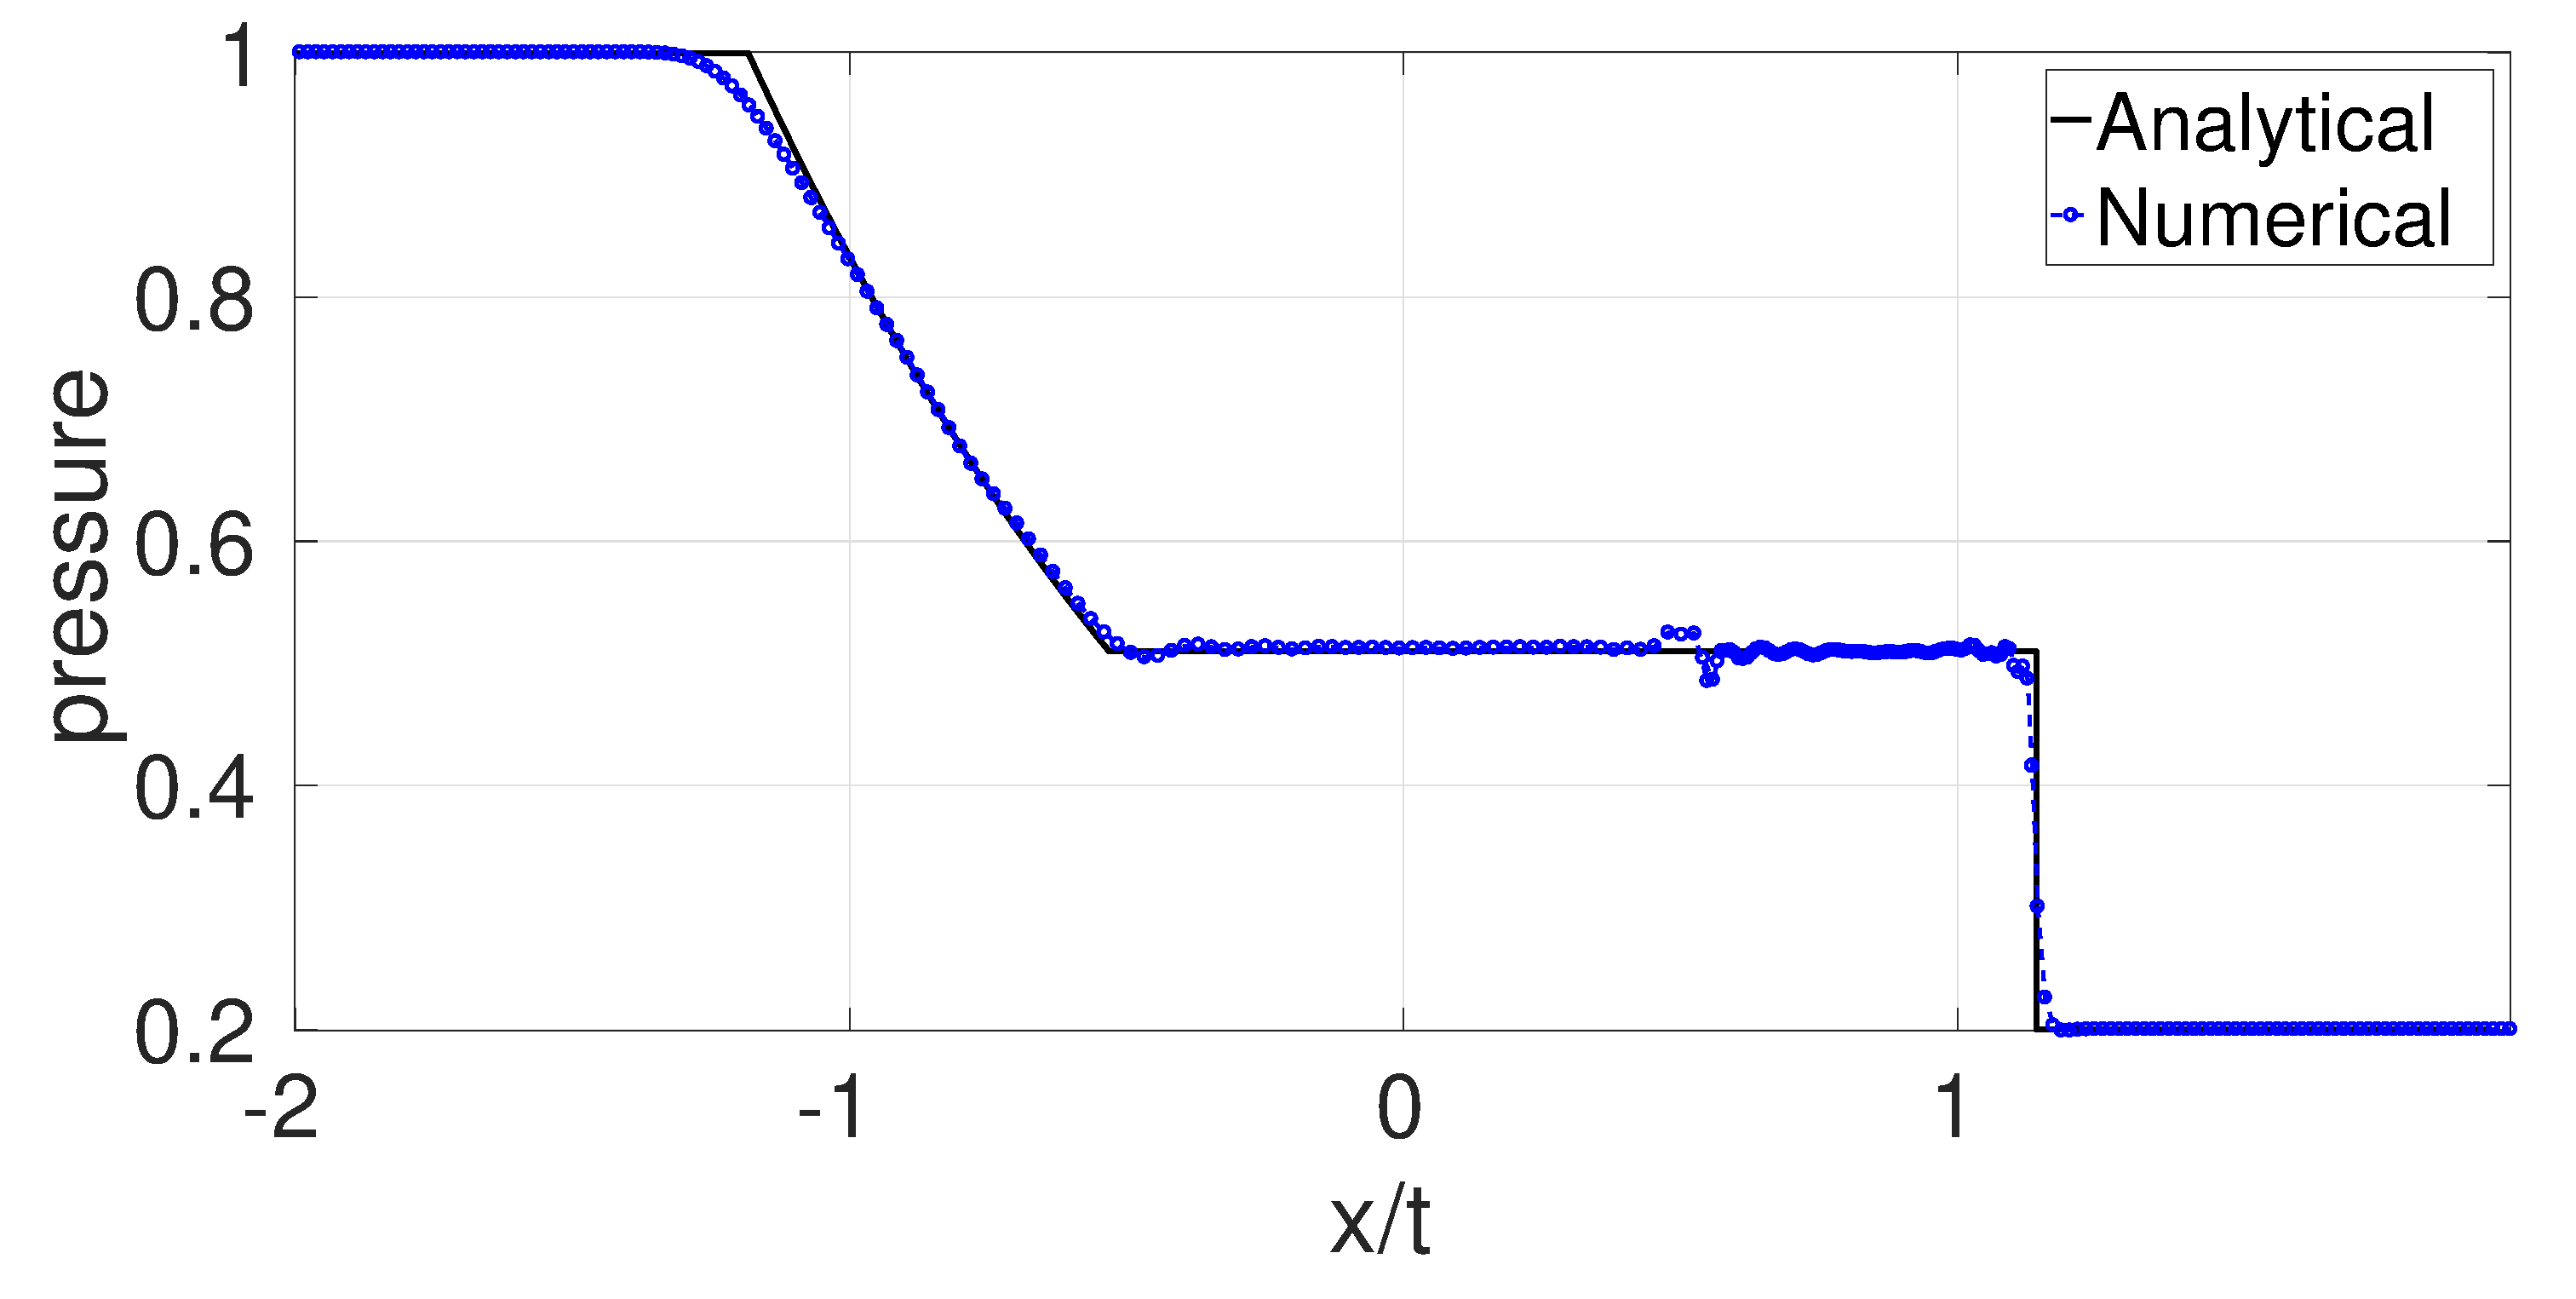
\includegraphics[width=0.99 \textwidth]{Chapter-4/Figures/GSPH-Sod/GRod-RCM-p}
    \end{minipage}% 
    \caption{Results for test 2, a variation of Sod test. All physical properties are well re-produced except for some acceptable oscillations}
    \label{fig:RCM-GSPH-Sod}
\end{figure}

\begin{figure}[H]
    \centering
    \begin{minipage}{.495\textwidth}
        \centering
        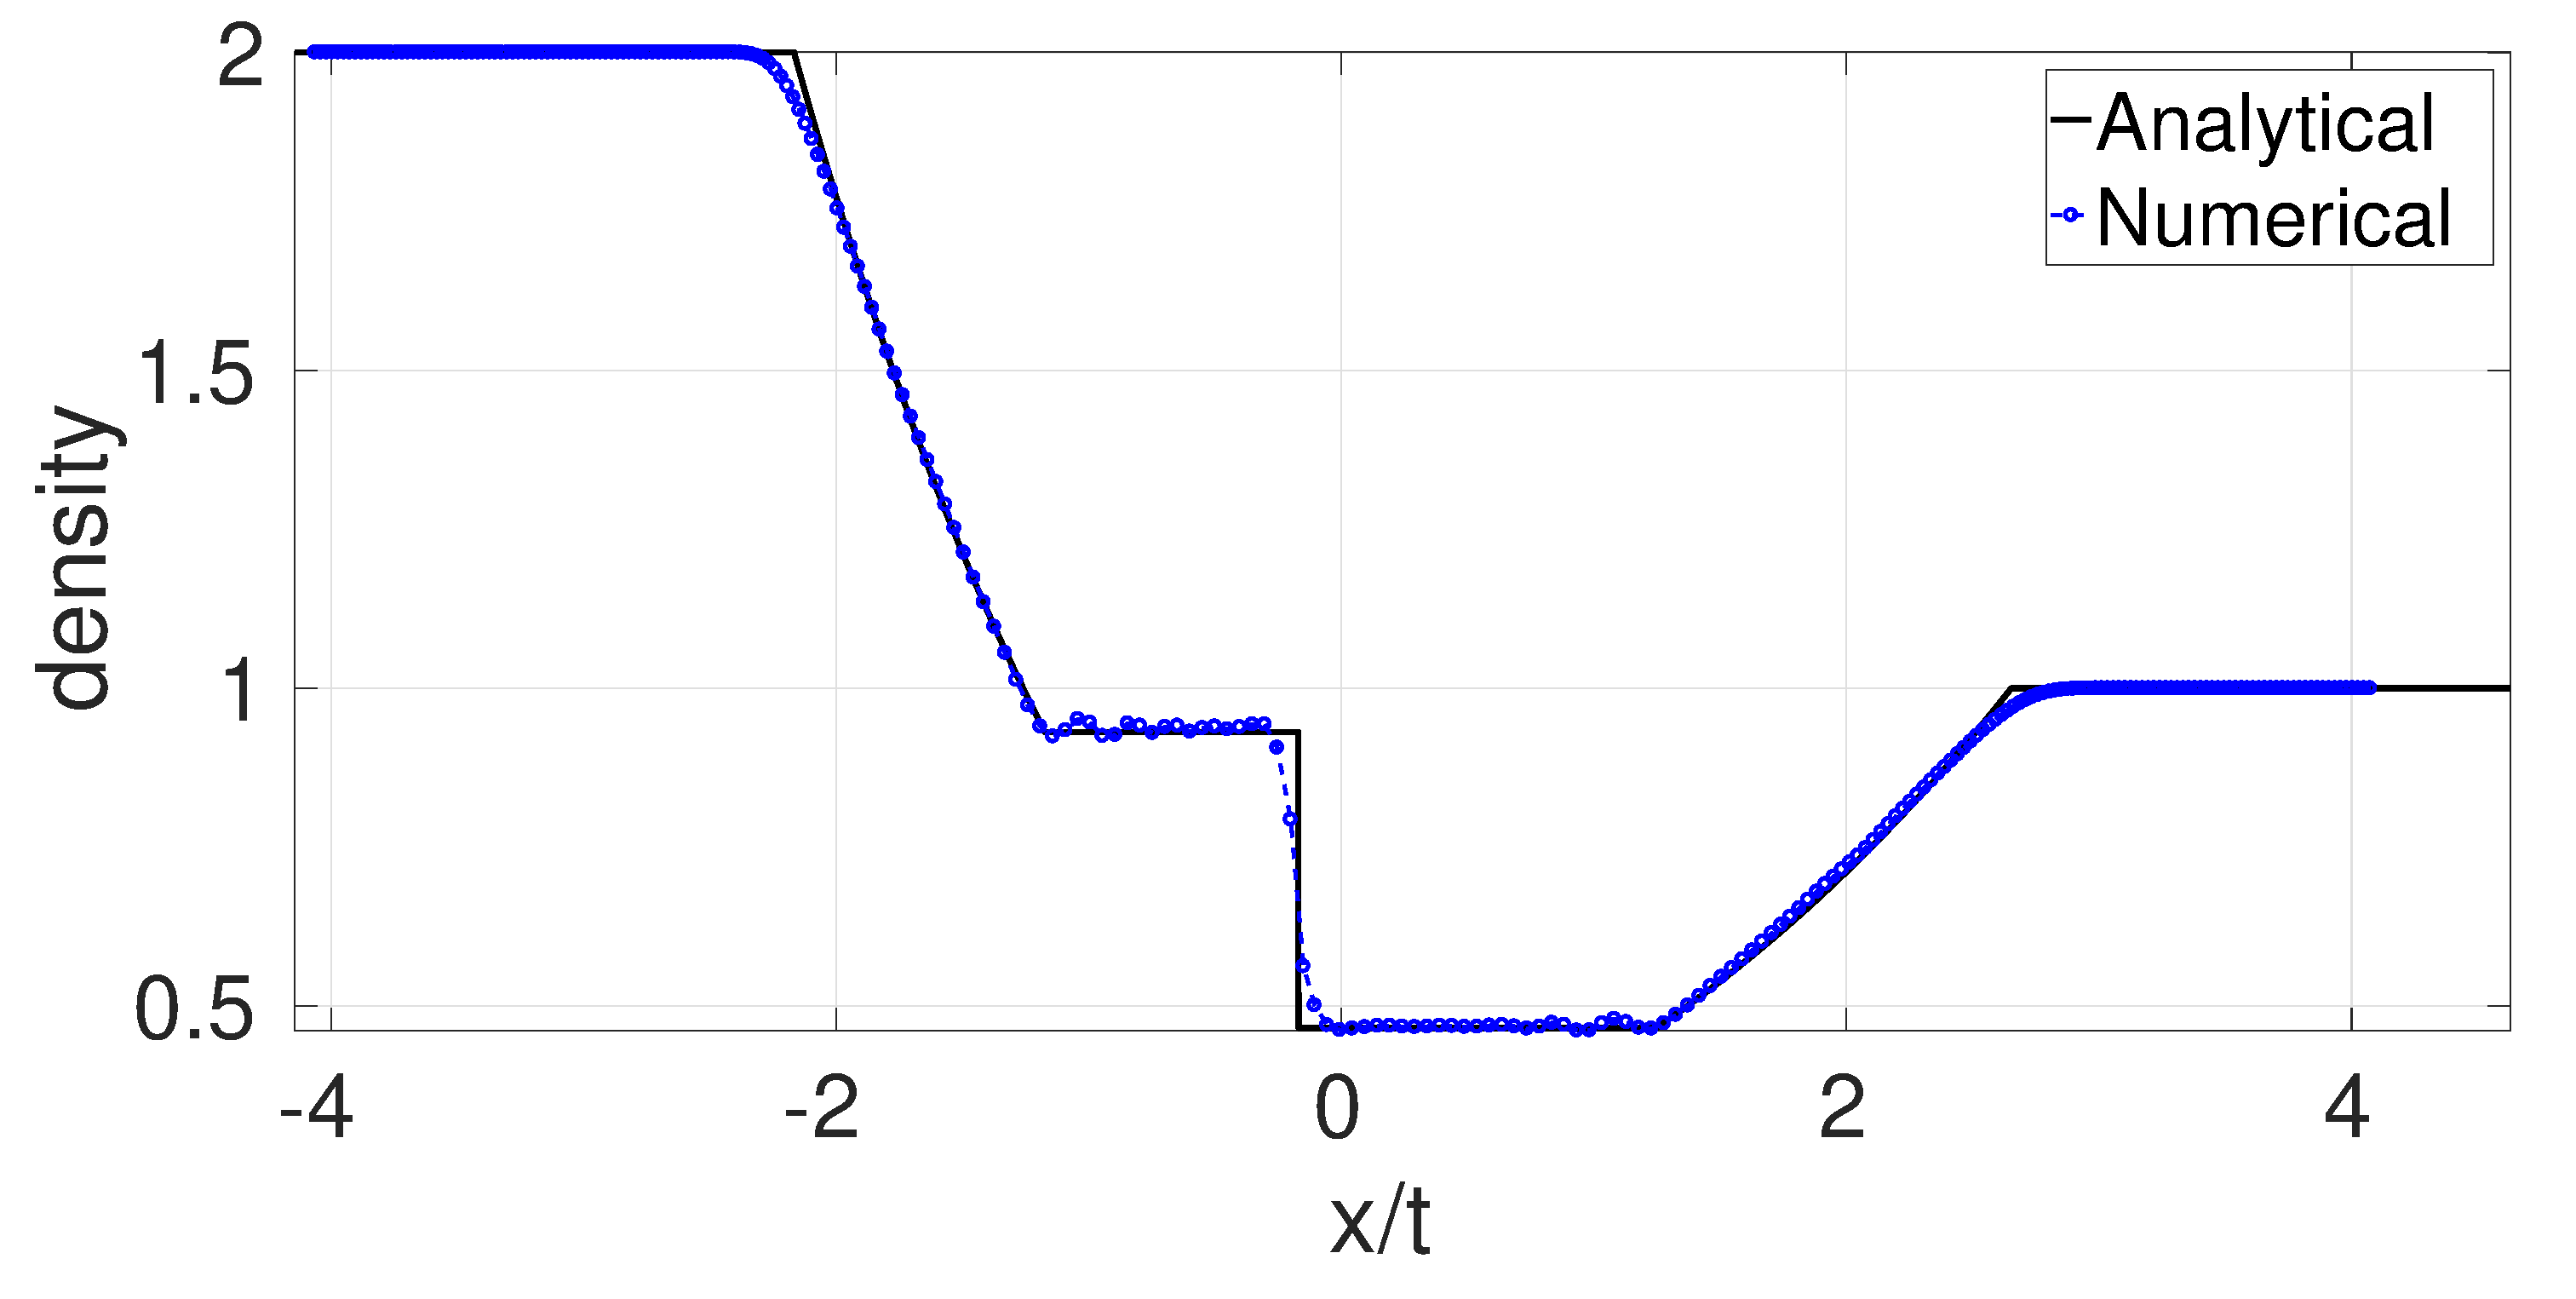
\includegraphics[width=0.99 \textwidth]{Chapter-4/Figures/double_exp/Dexp-RCM-rho}
    \end{minipage}%
    \begin{minipage}{.495 \textwidth}
        \centering
        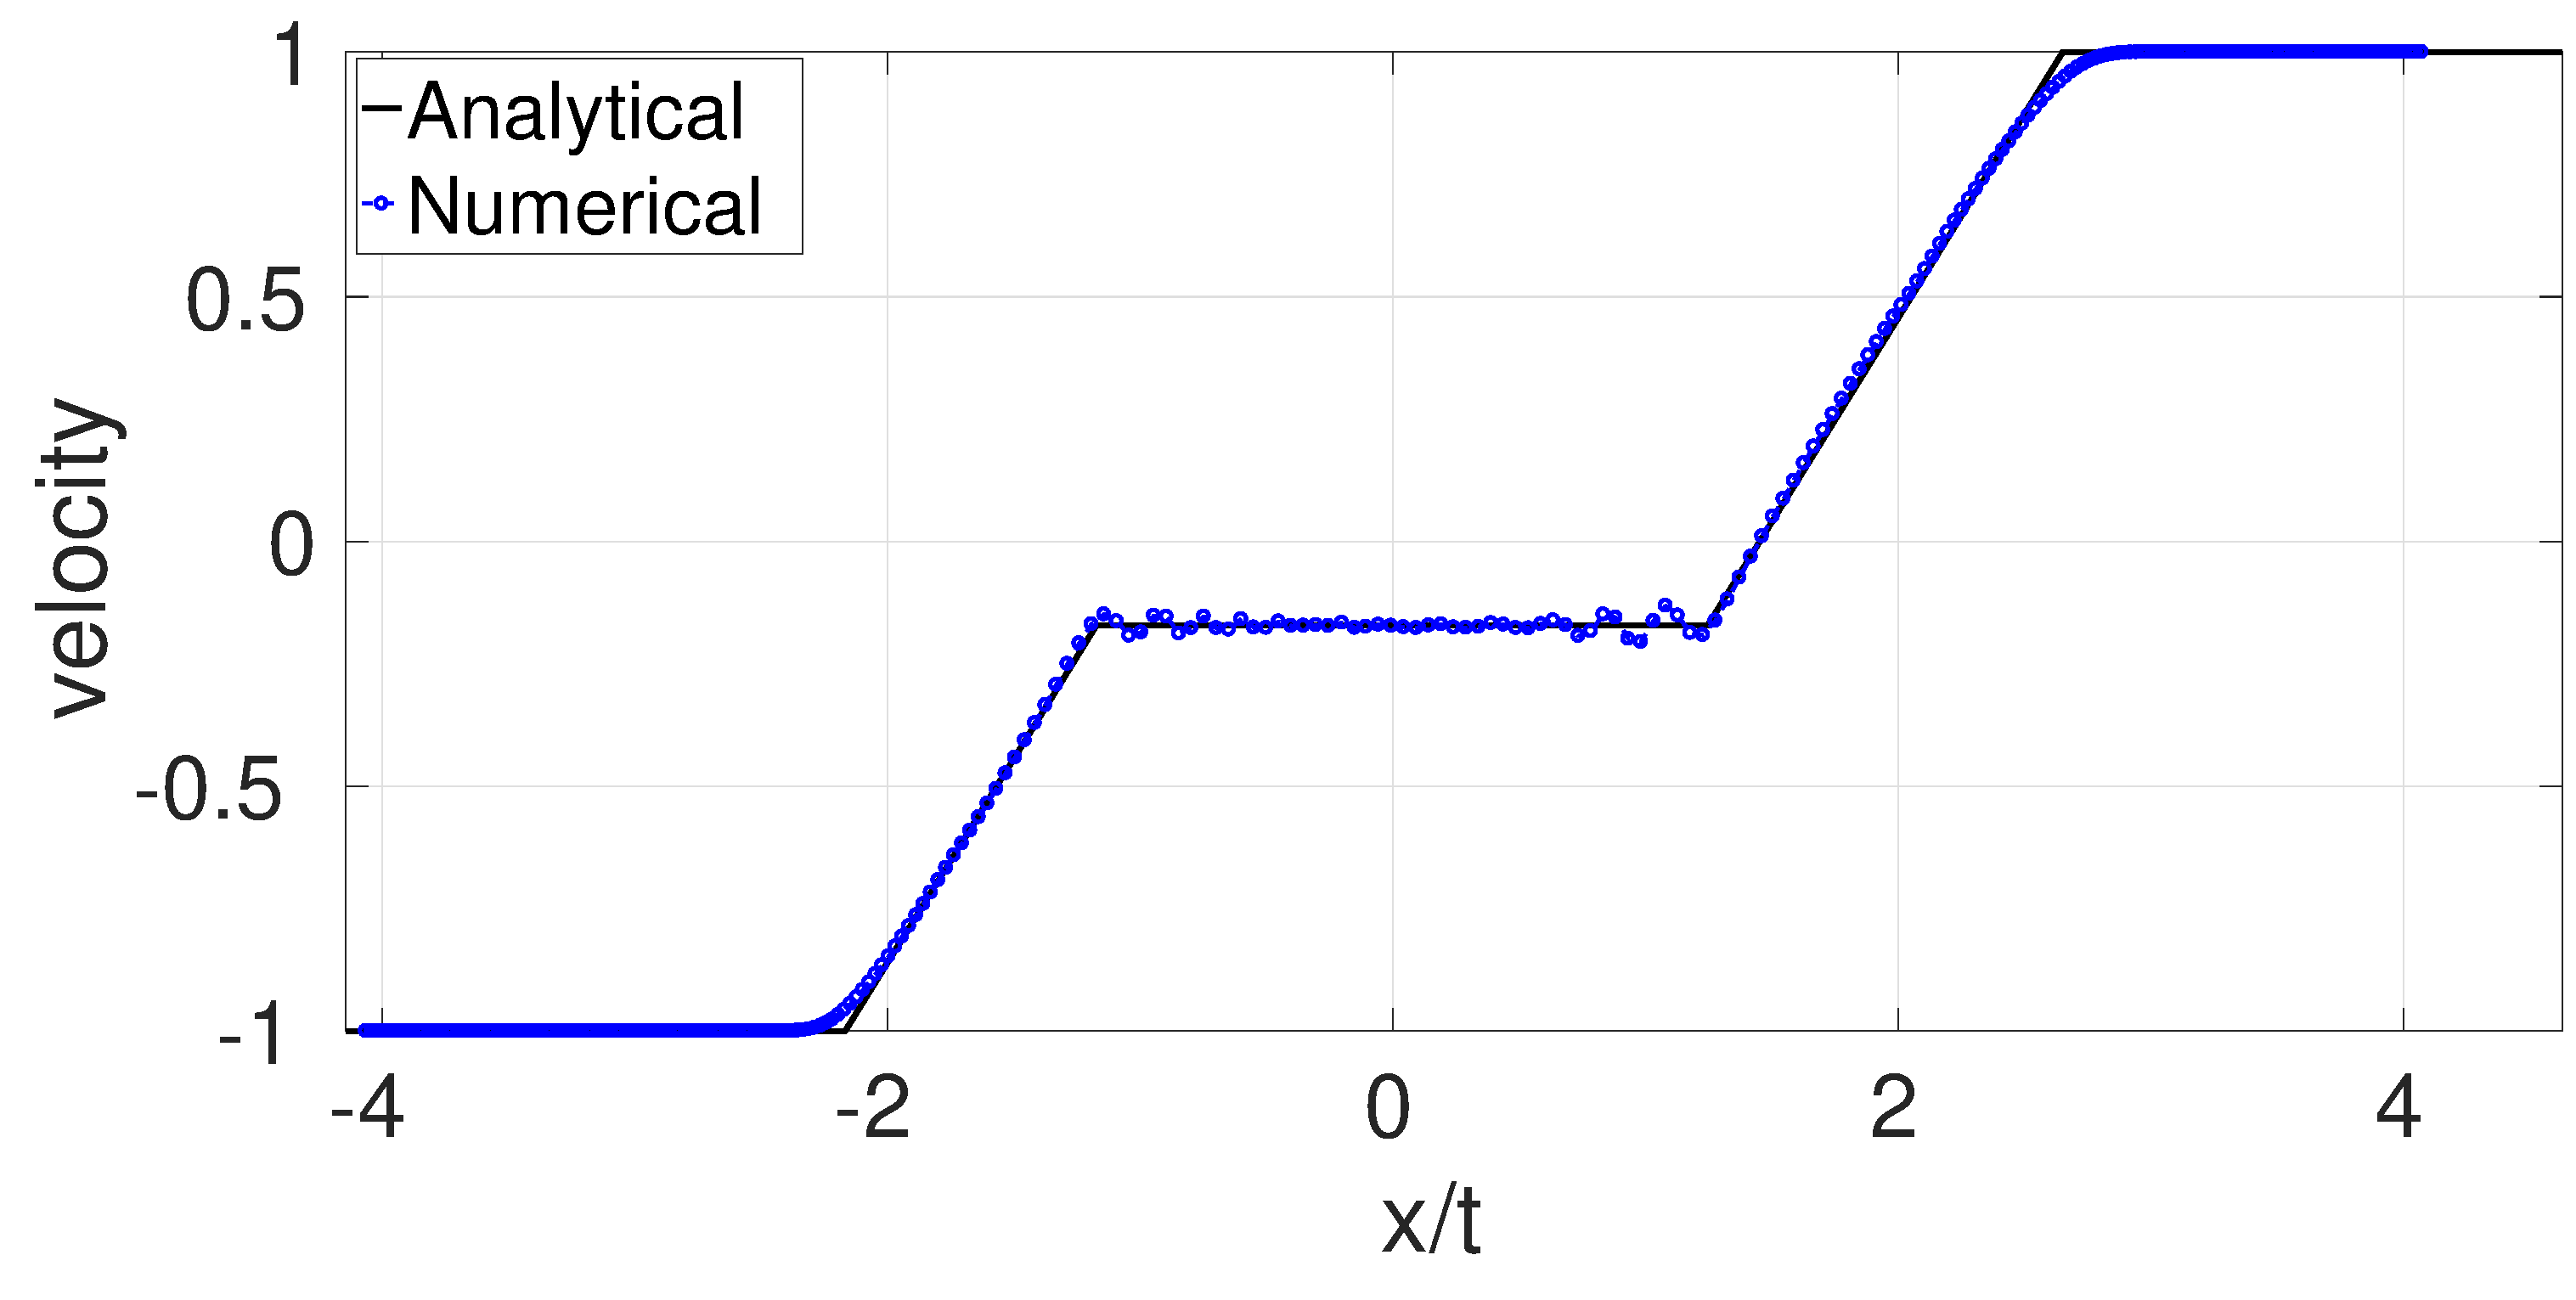
\includegraphics[width=0.99 \textwidth]{Chapter-4/Figures/double_exp/Dexp-RCM-v}
    \end{minipage}%
    \\
    \begin{minipage}{.495\textwidth}
        \centering
        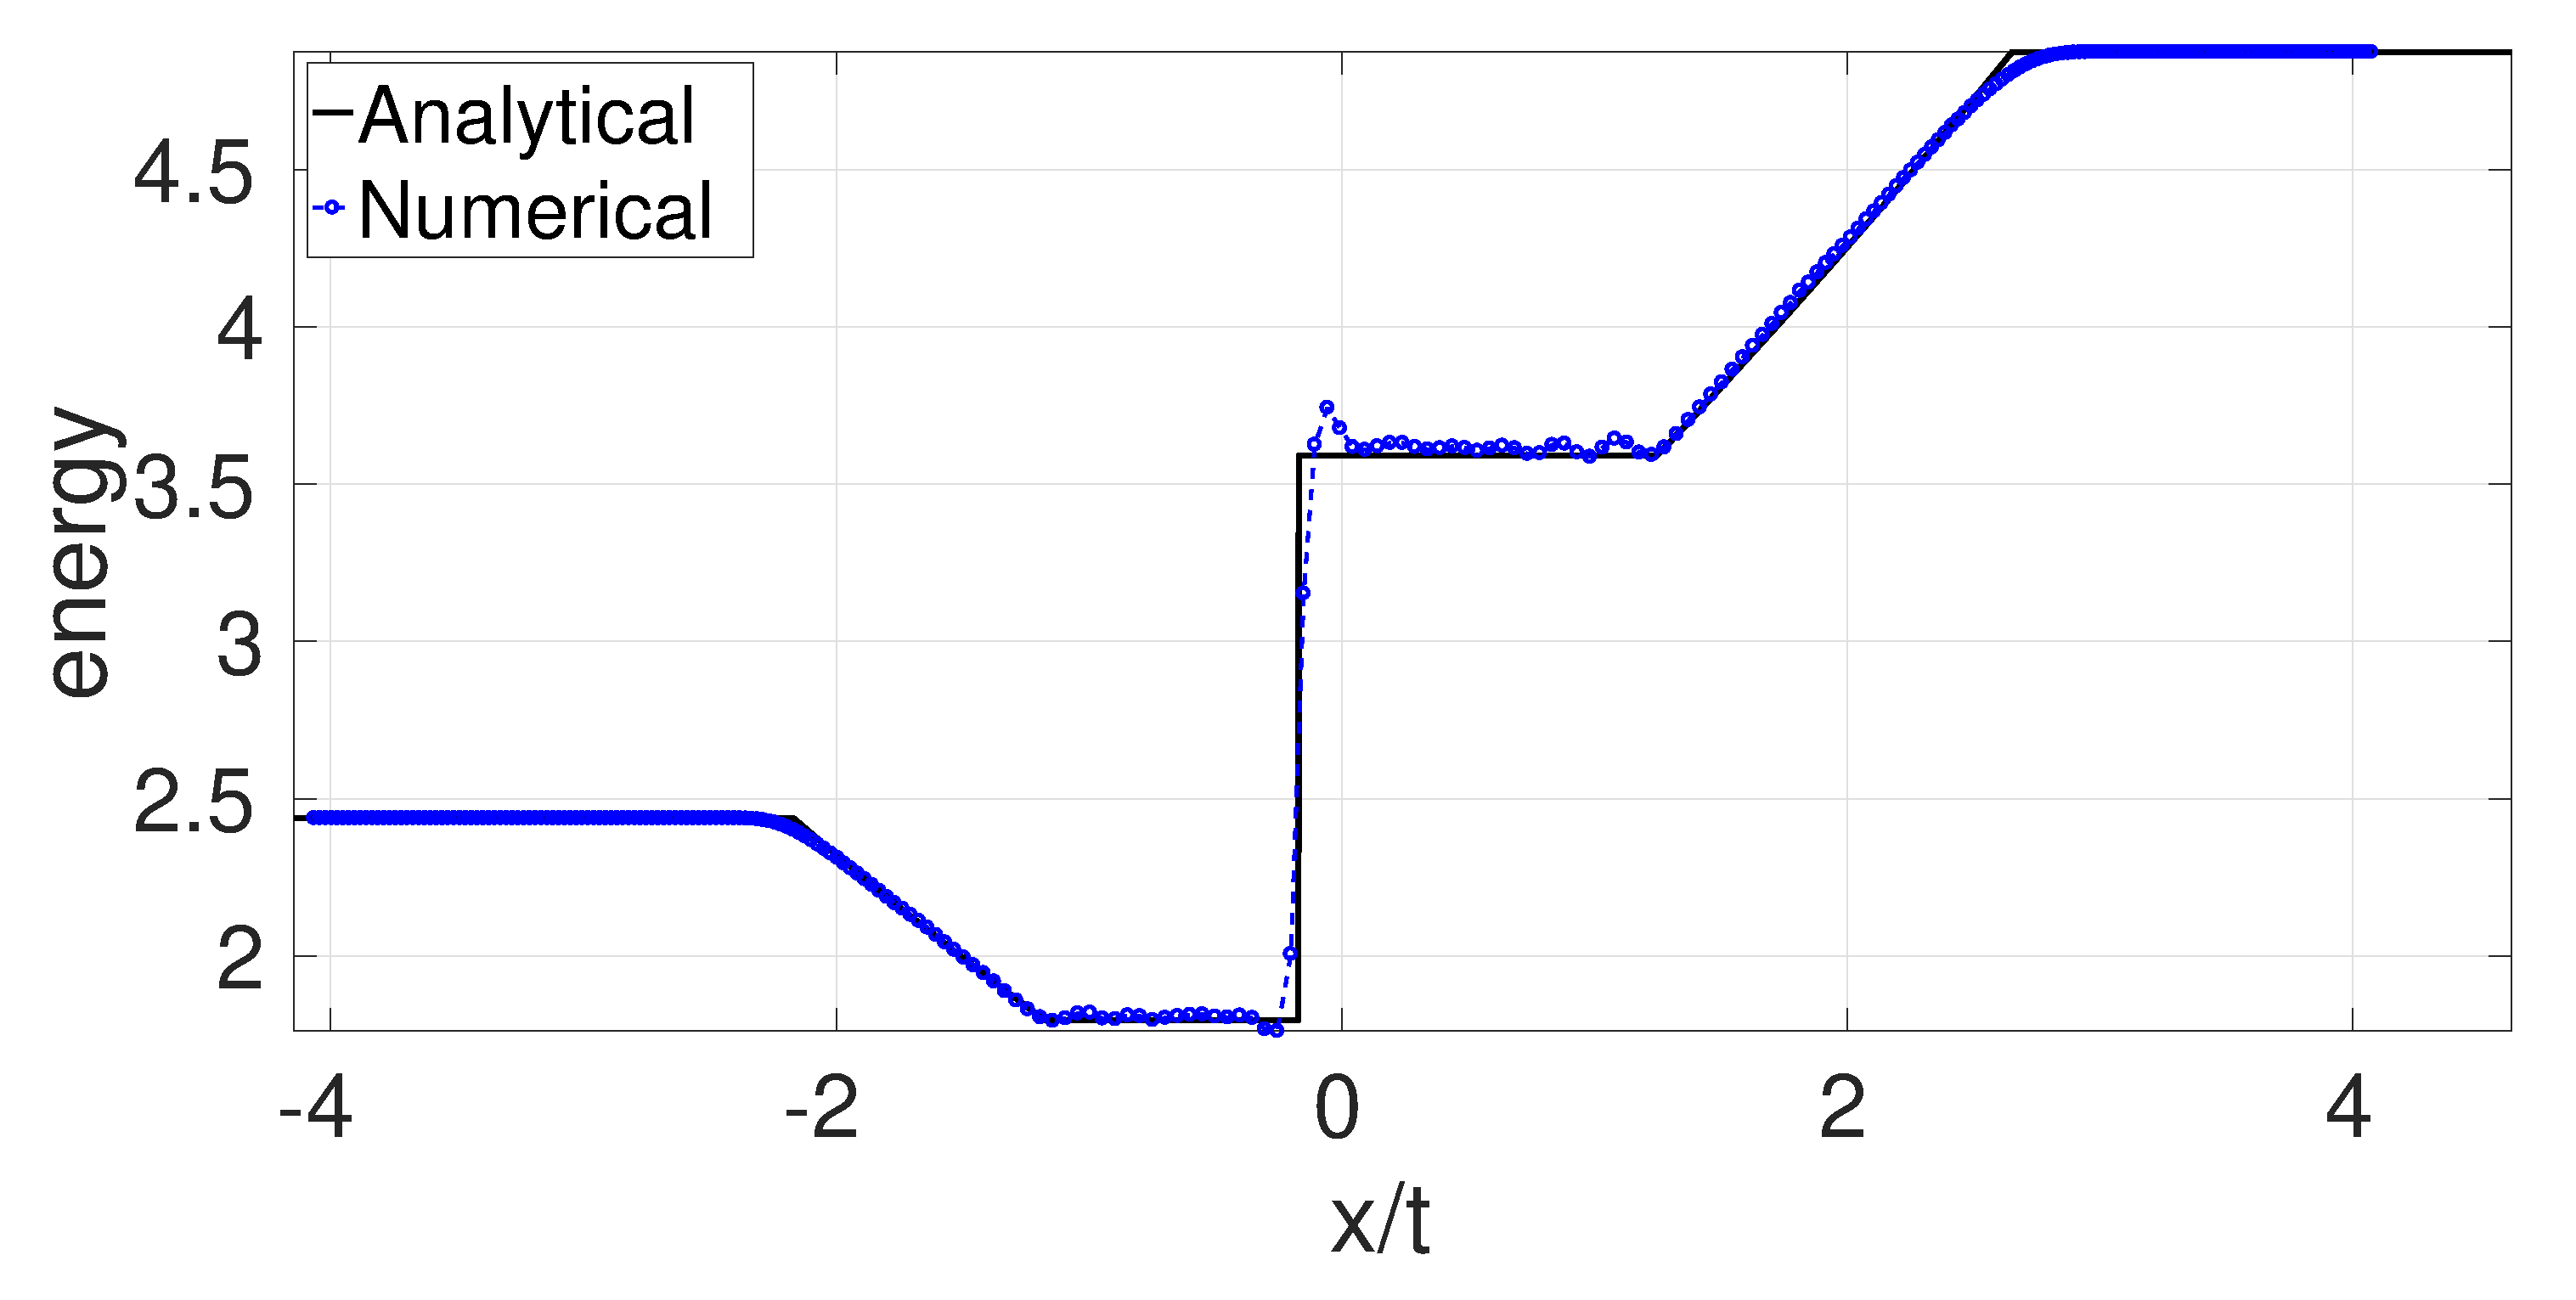
\includegraphics[width=0.99 \textwidth]{Chapter-4/Figures/double_exp/Dexp-RCM-e}
    \end{minipage}%
    \begin{minipage}{.495 \textwidth}
        \centering
        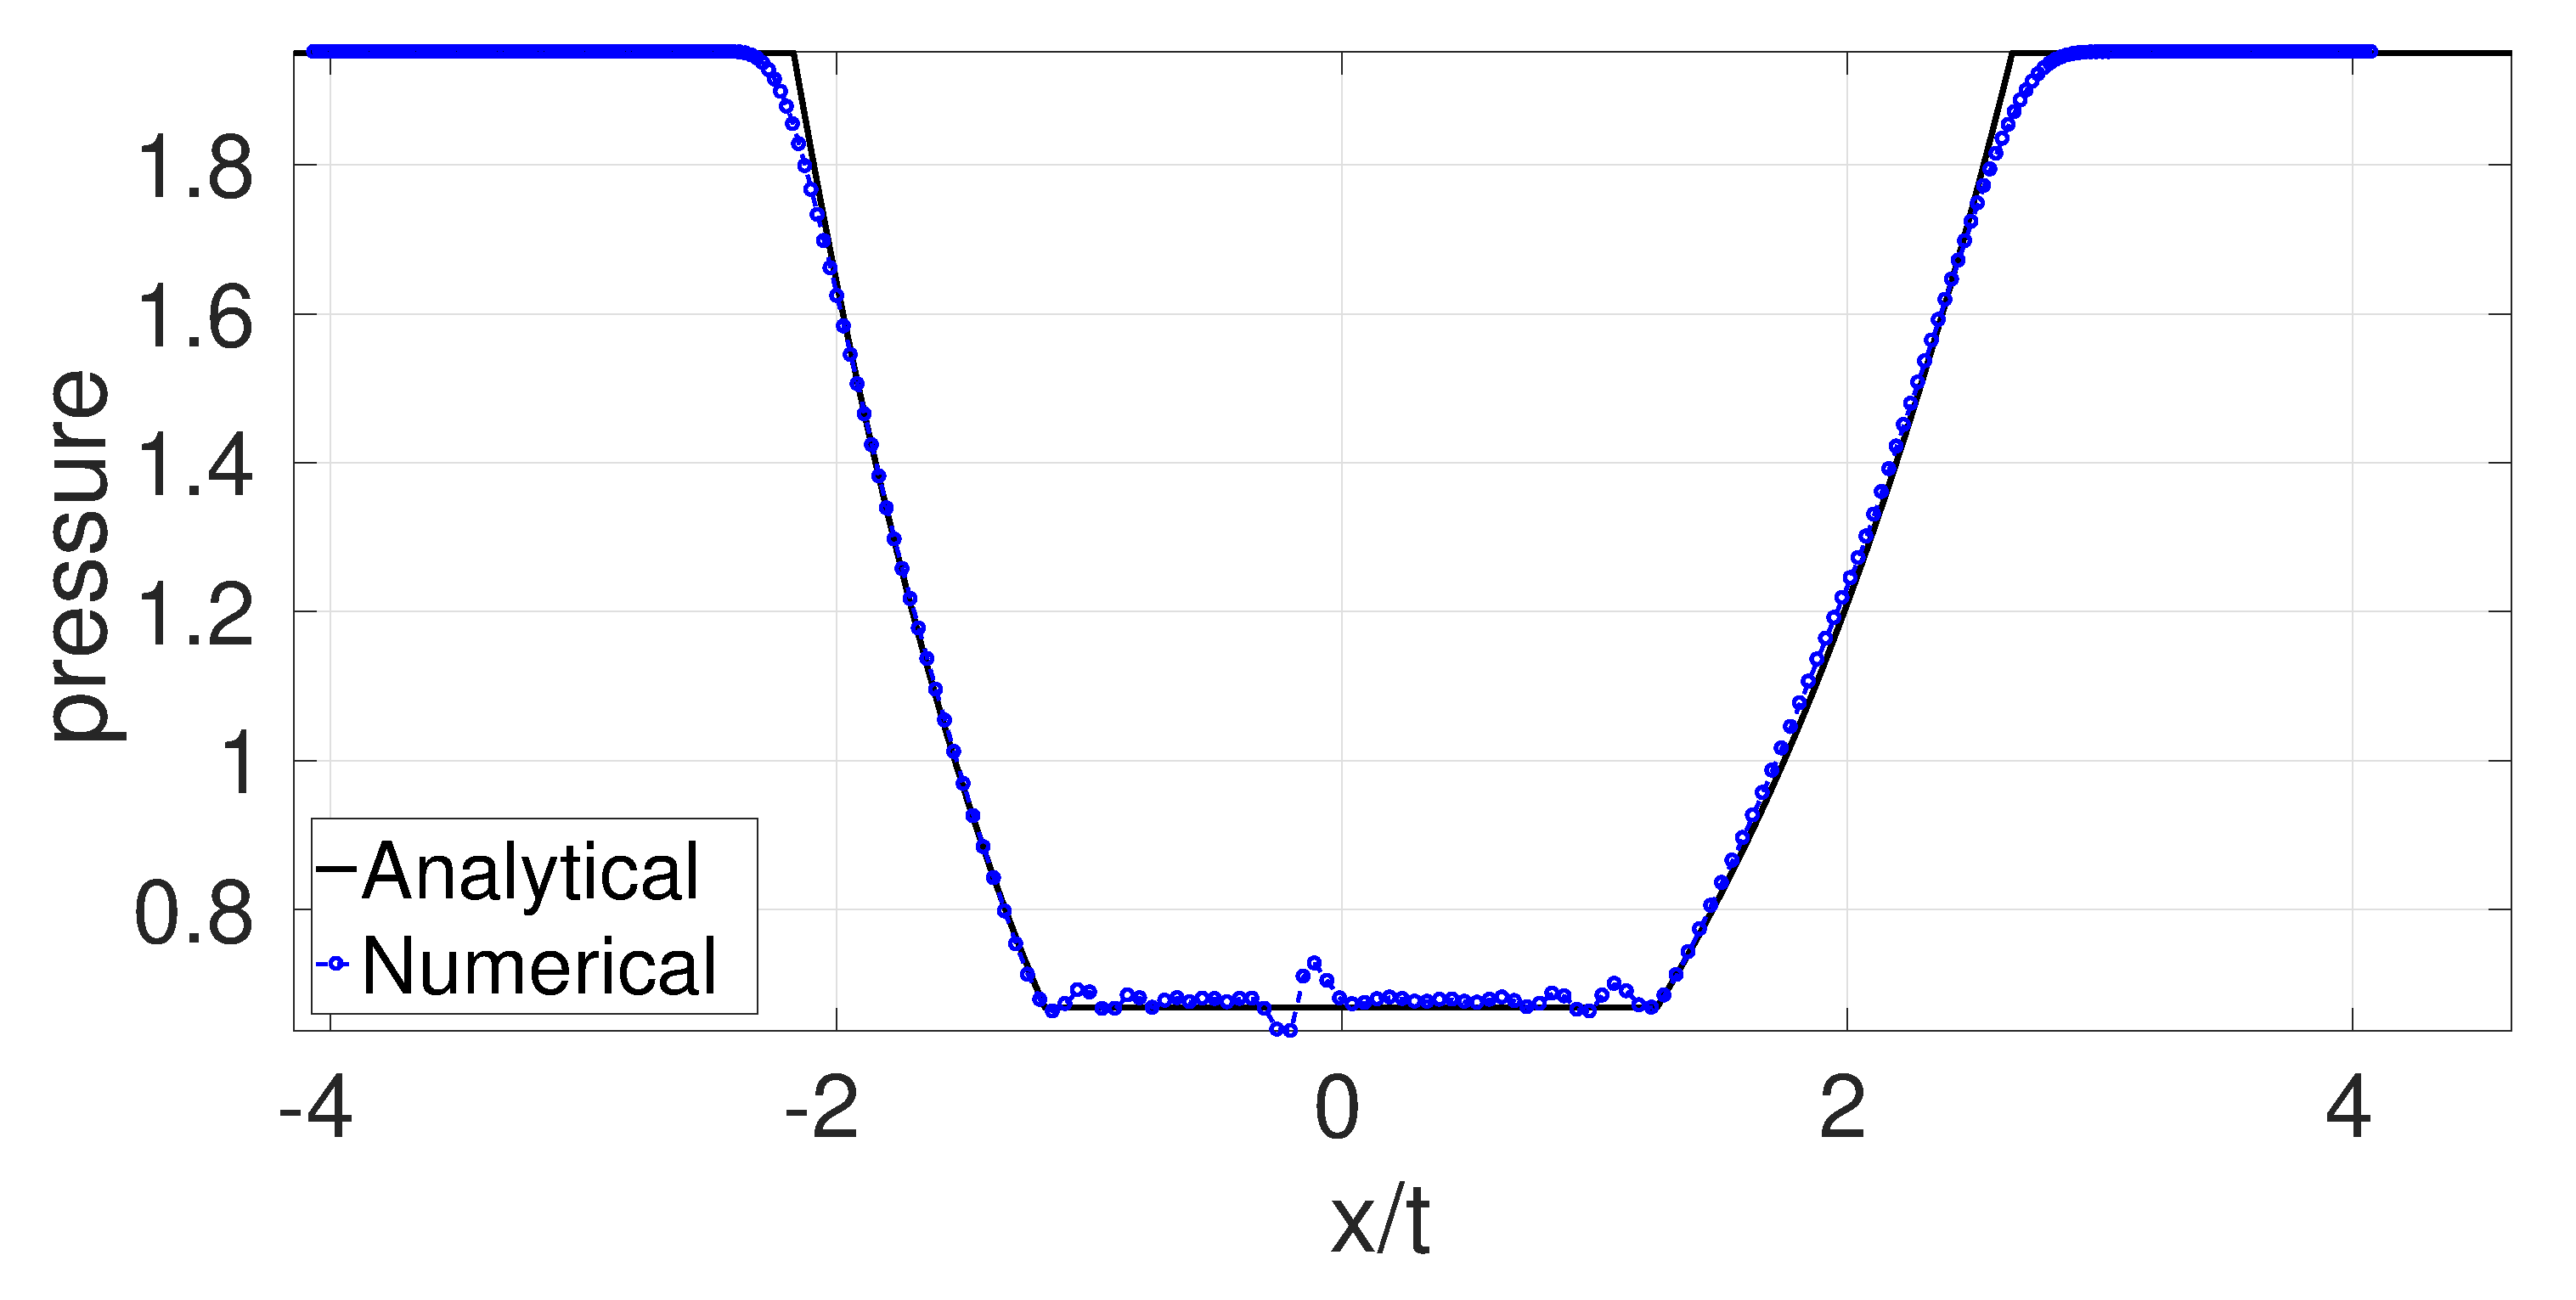
\includegraphics[width=0.99 \textwidth]{Chapter-4/Figures/double_exp/Dexp-RCM-p}
    \end{minipage}% 
    \caption{Results for test 3, the double expansion case. All physical properties are well re-produced except for some oscillations}
    \label{fig:RCM-double-expansion}
\end{figure}

\begin{figure}[H]
    %\centering
    \begin{minipage}{.495\textwidth}
        \centering
        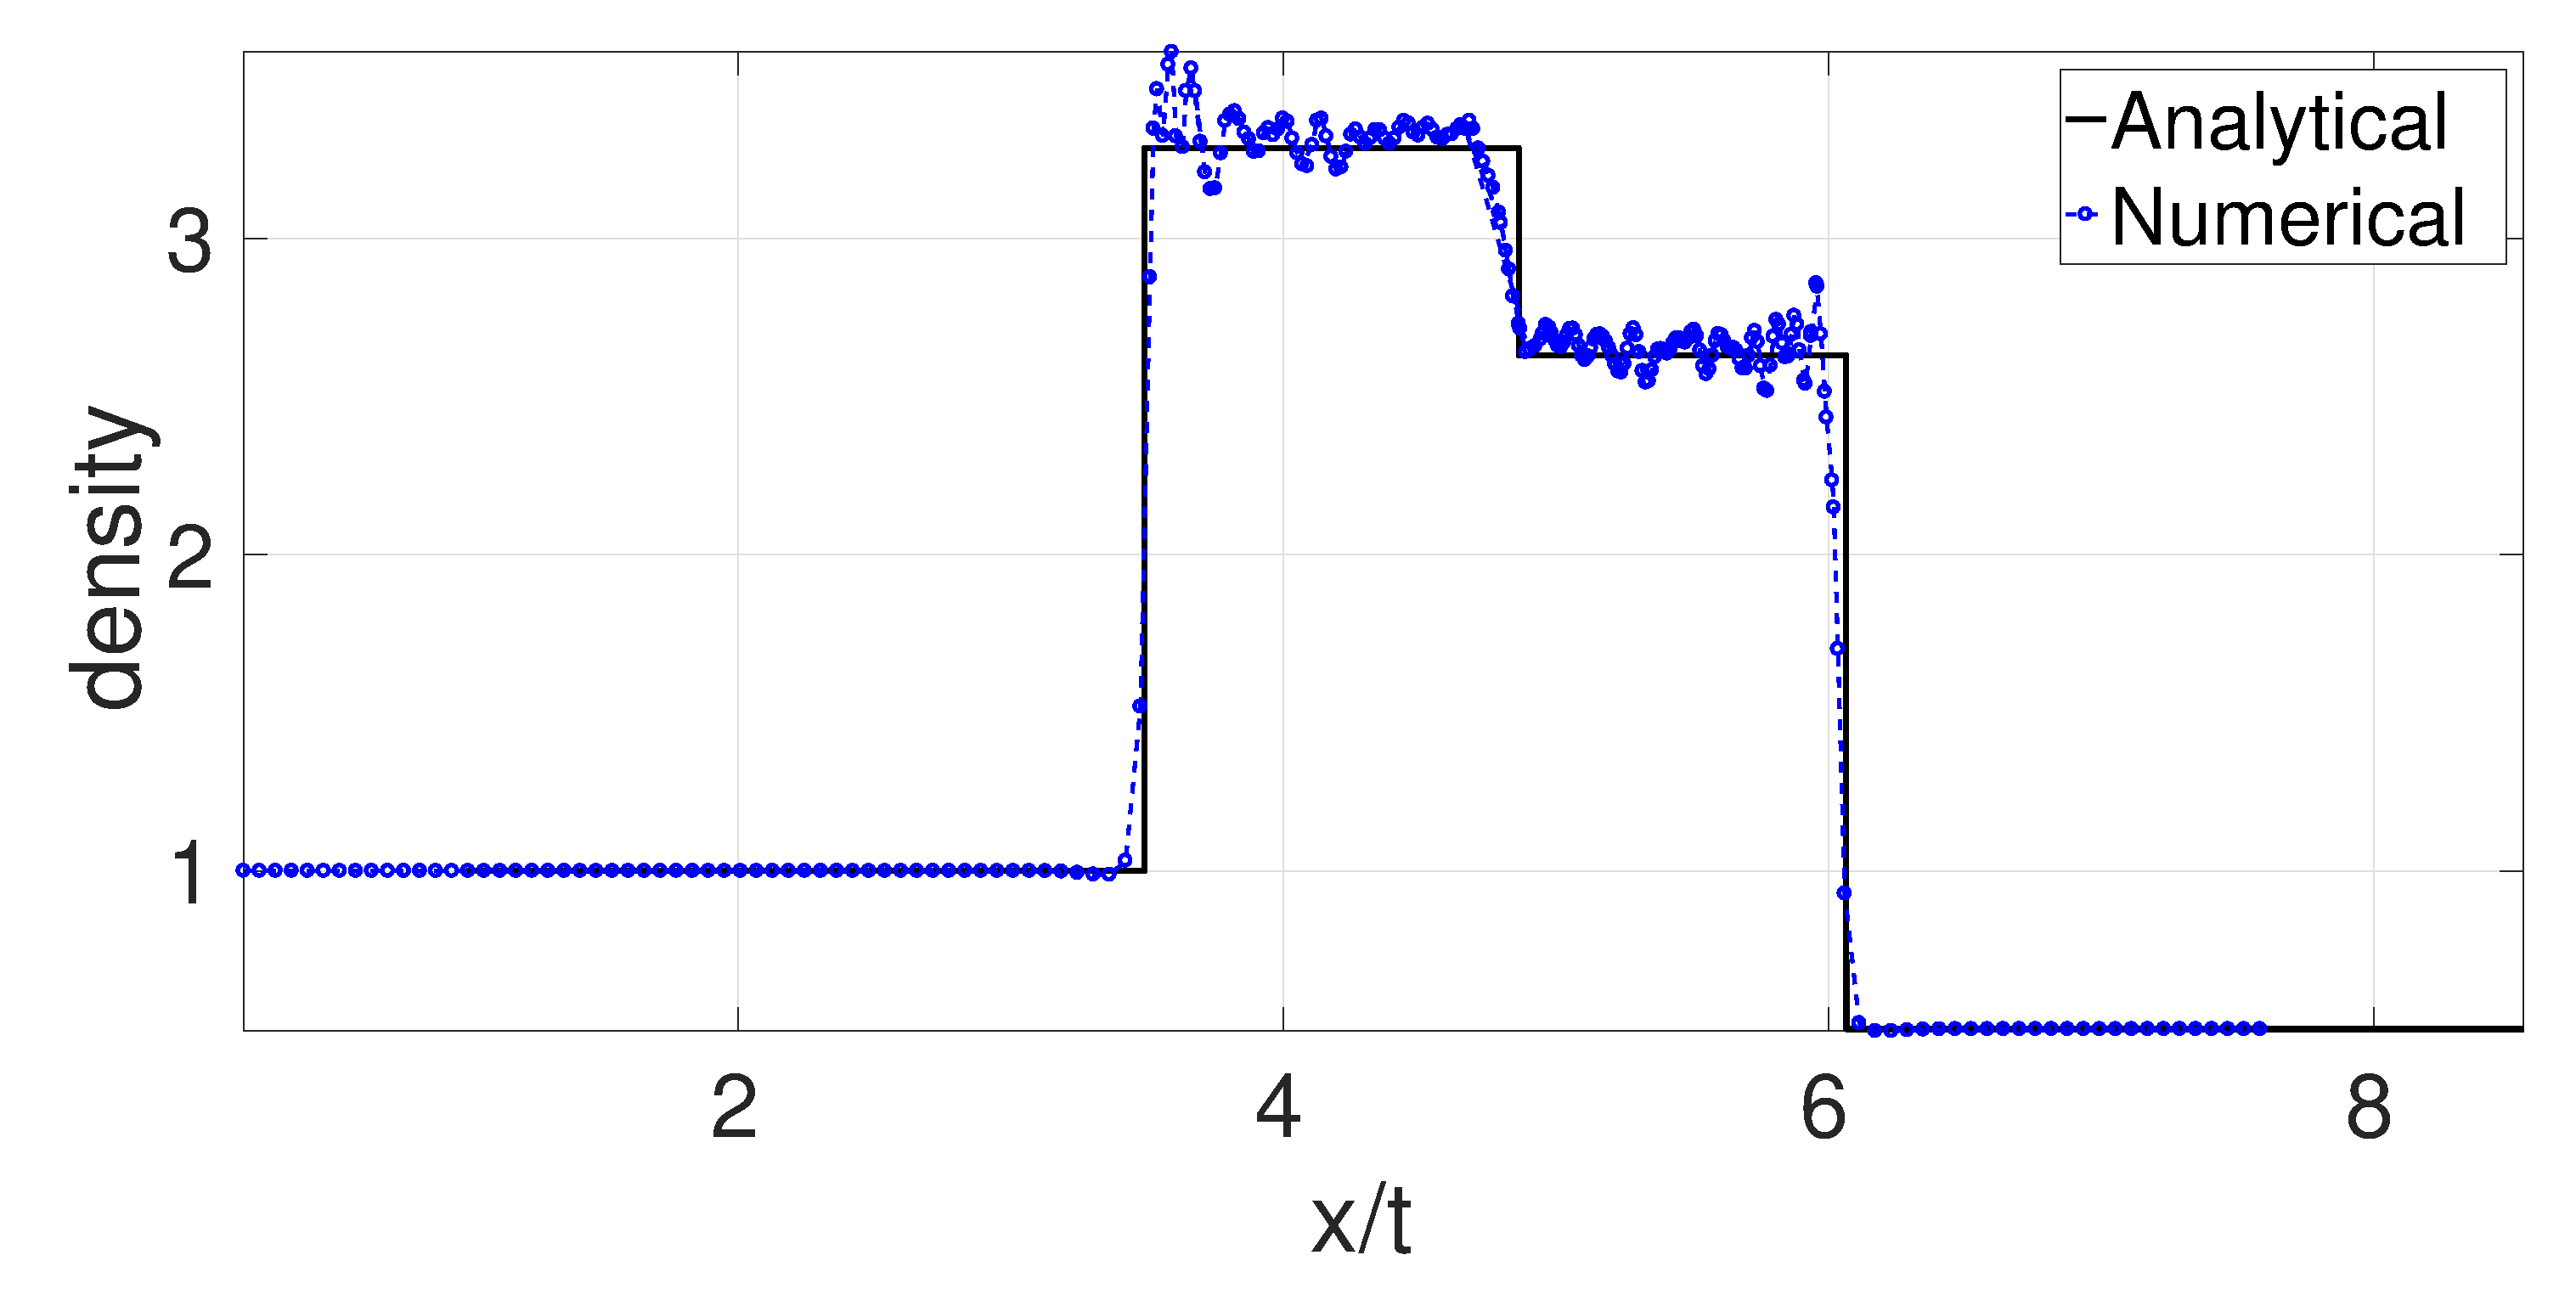
\includegraphics[width=0.99 \textwidth]{Chapter-4/Figures/double_shock/Dshock-RCM-rho-Rp6}
    \end{minipage}%
    \begin{minipage}{.495 \textwidth}
        \centering
        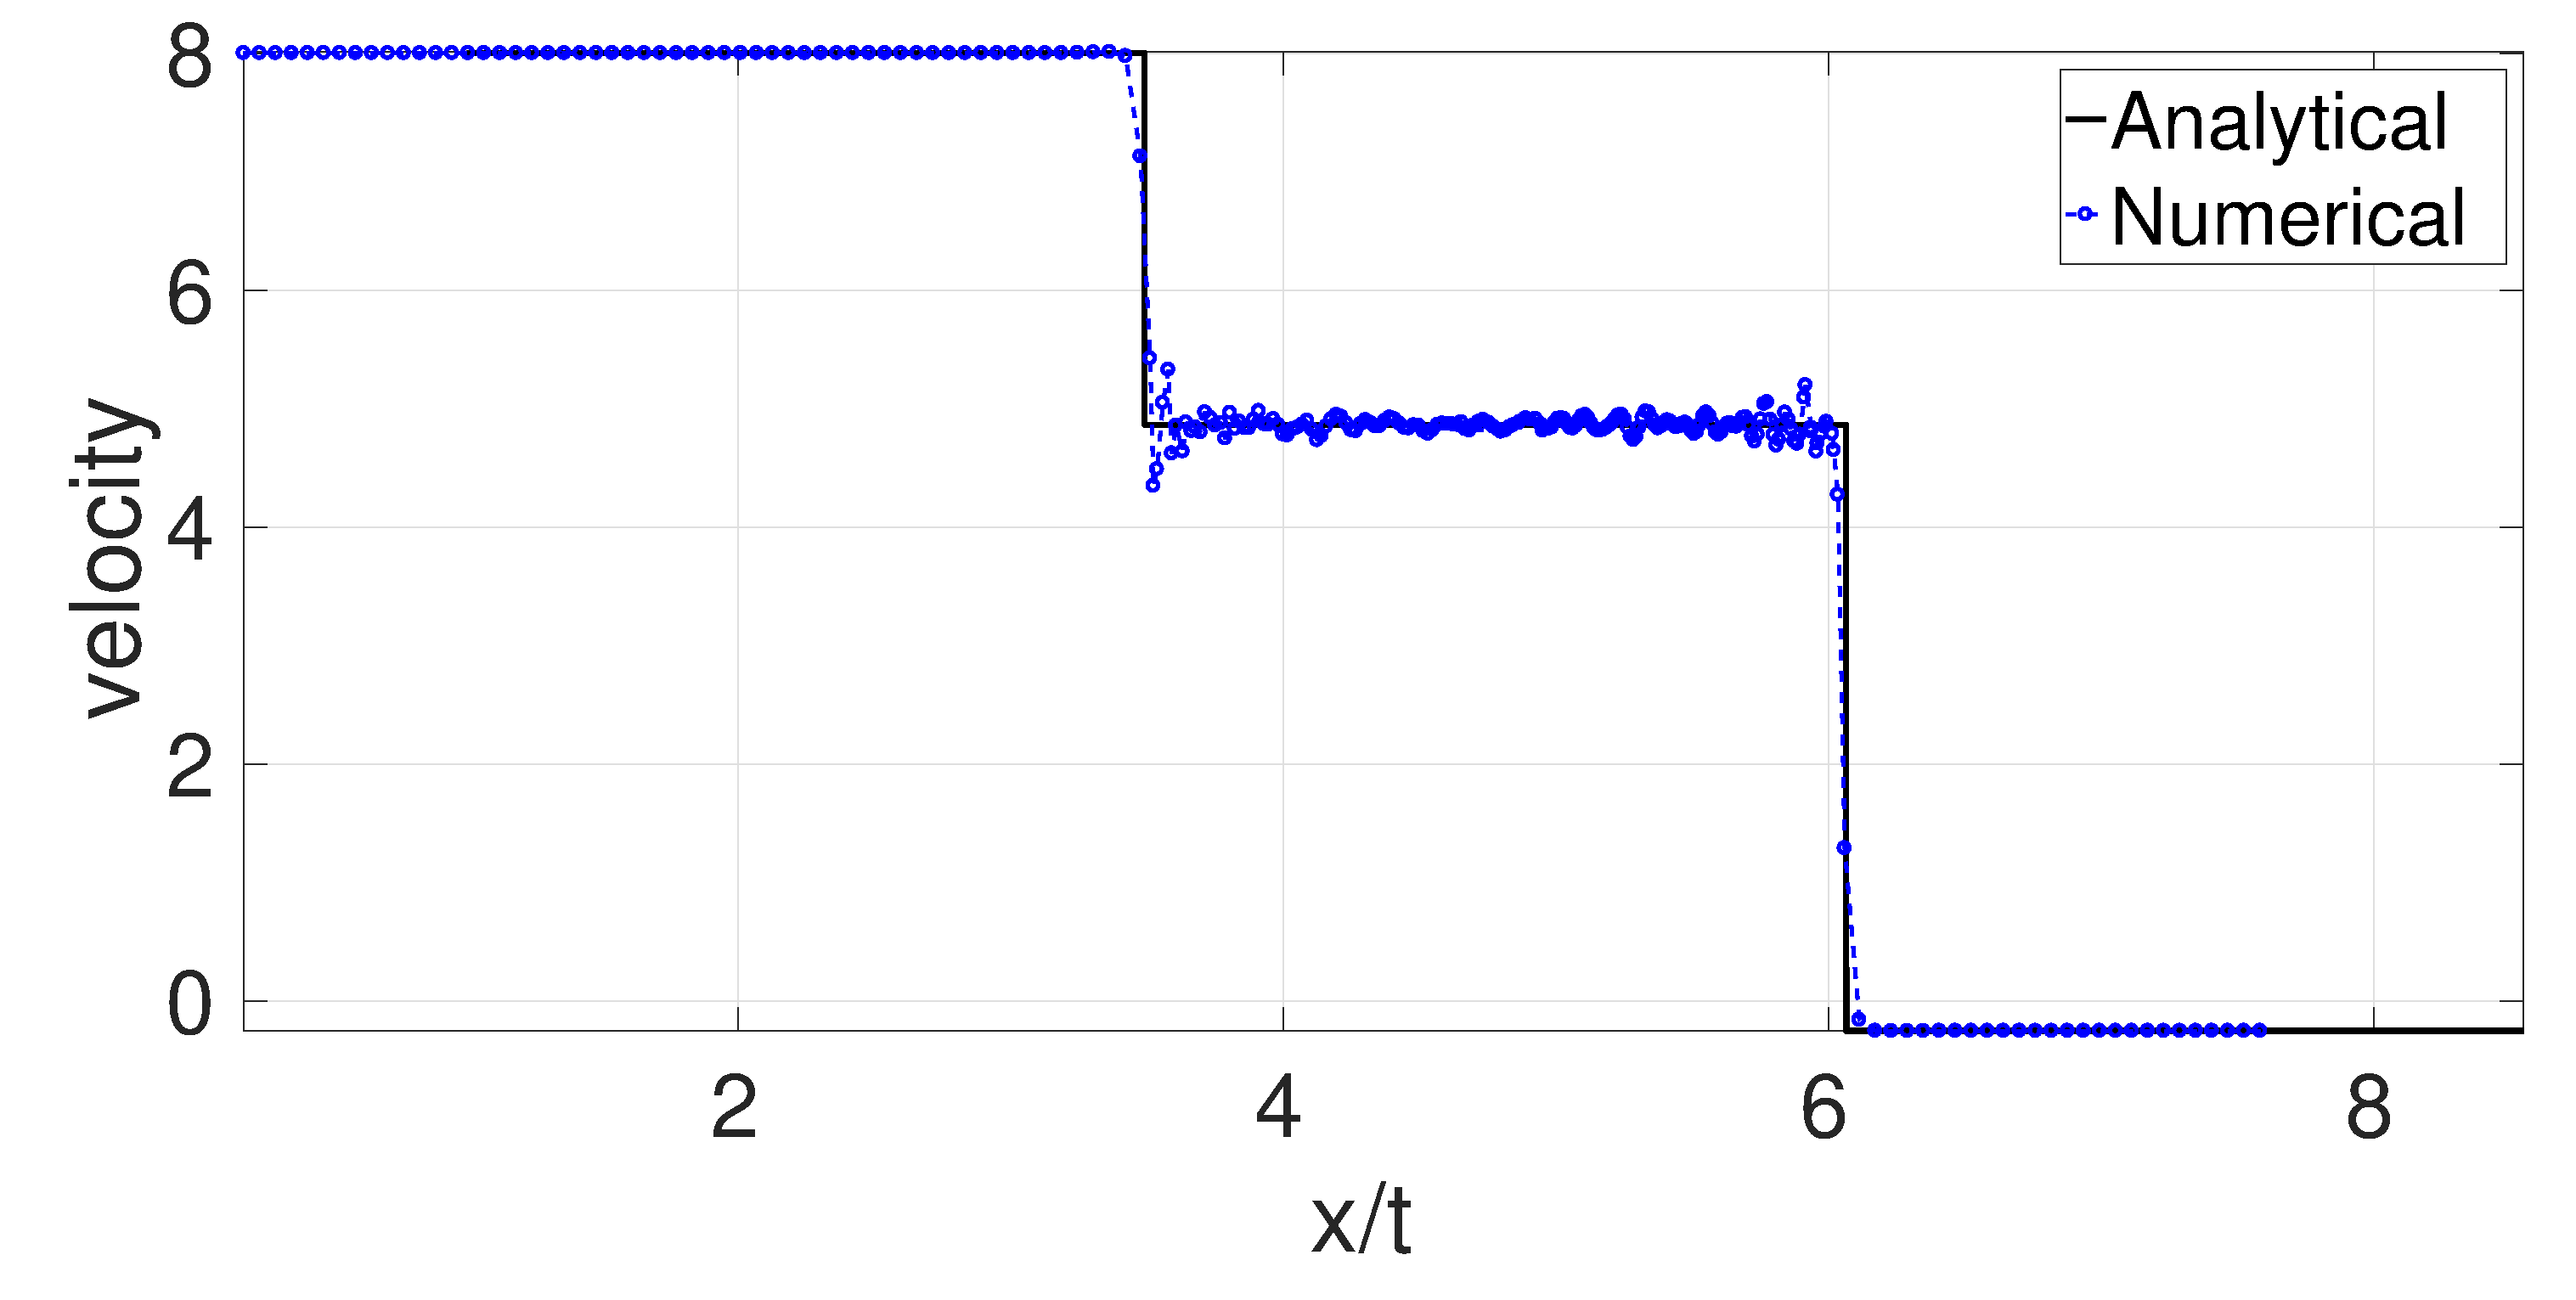
\includegraphics[width=0.99 \textwidth]{Chapter-4/Figures/double_shock/Dshock-RCM-v-Rp6}
    \end{minipage}%
    \\
    \begin{minipage}{.495\textwidth}
        \centering
        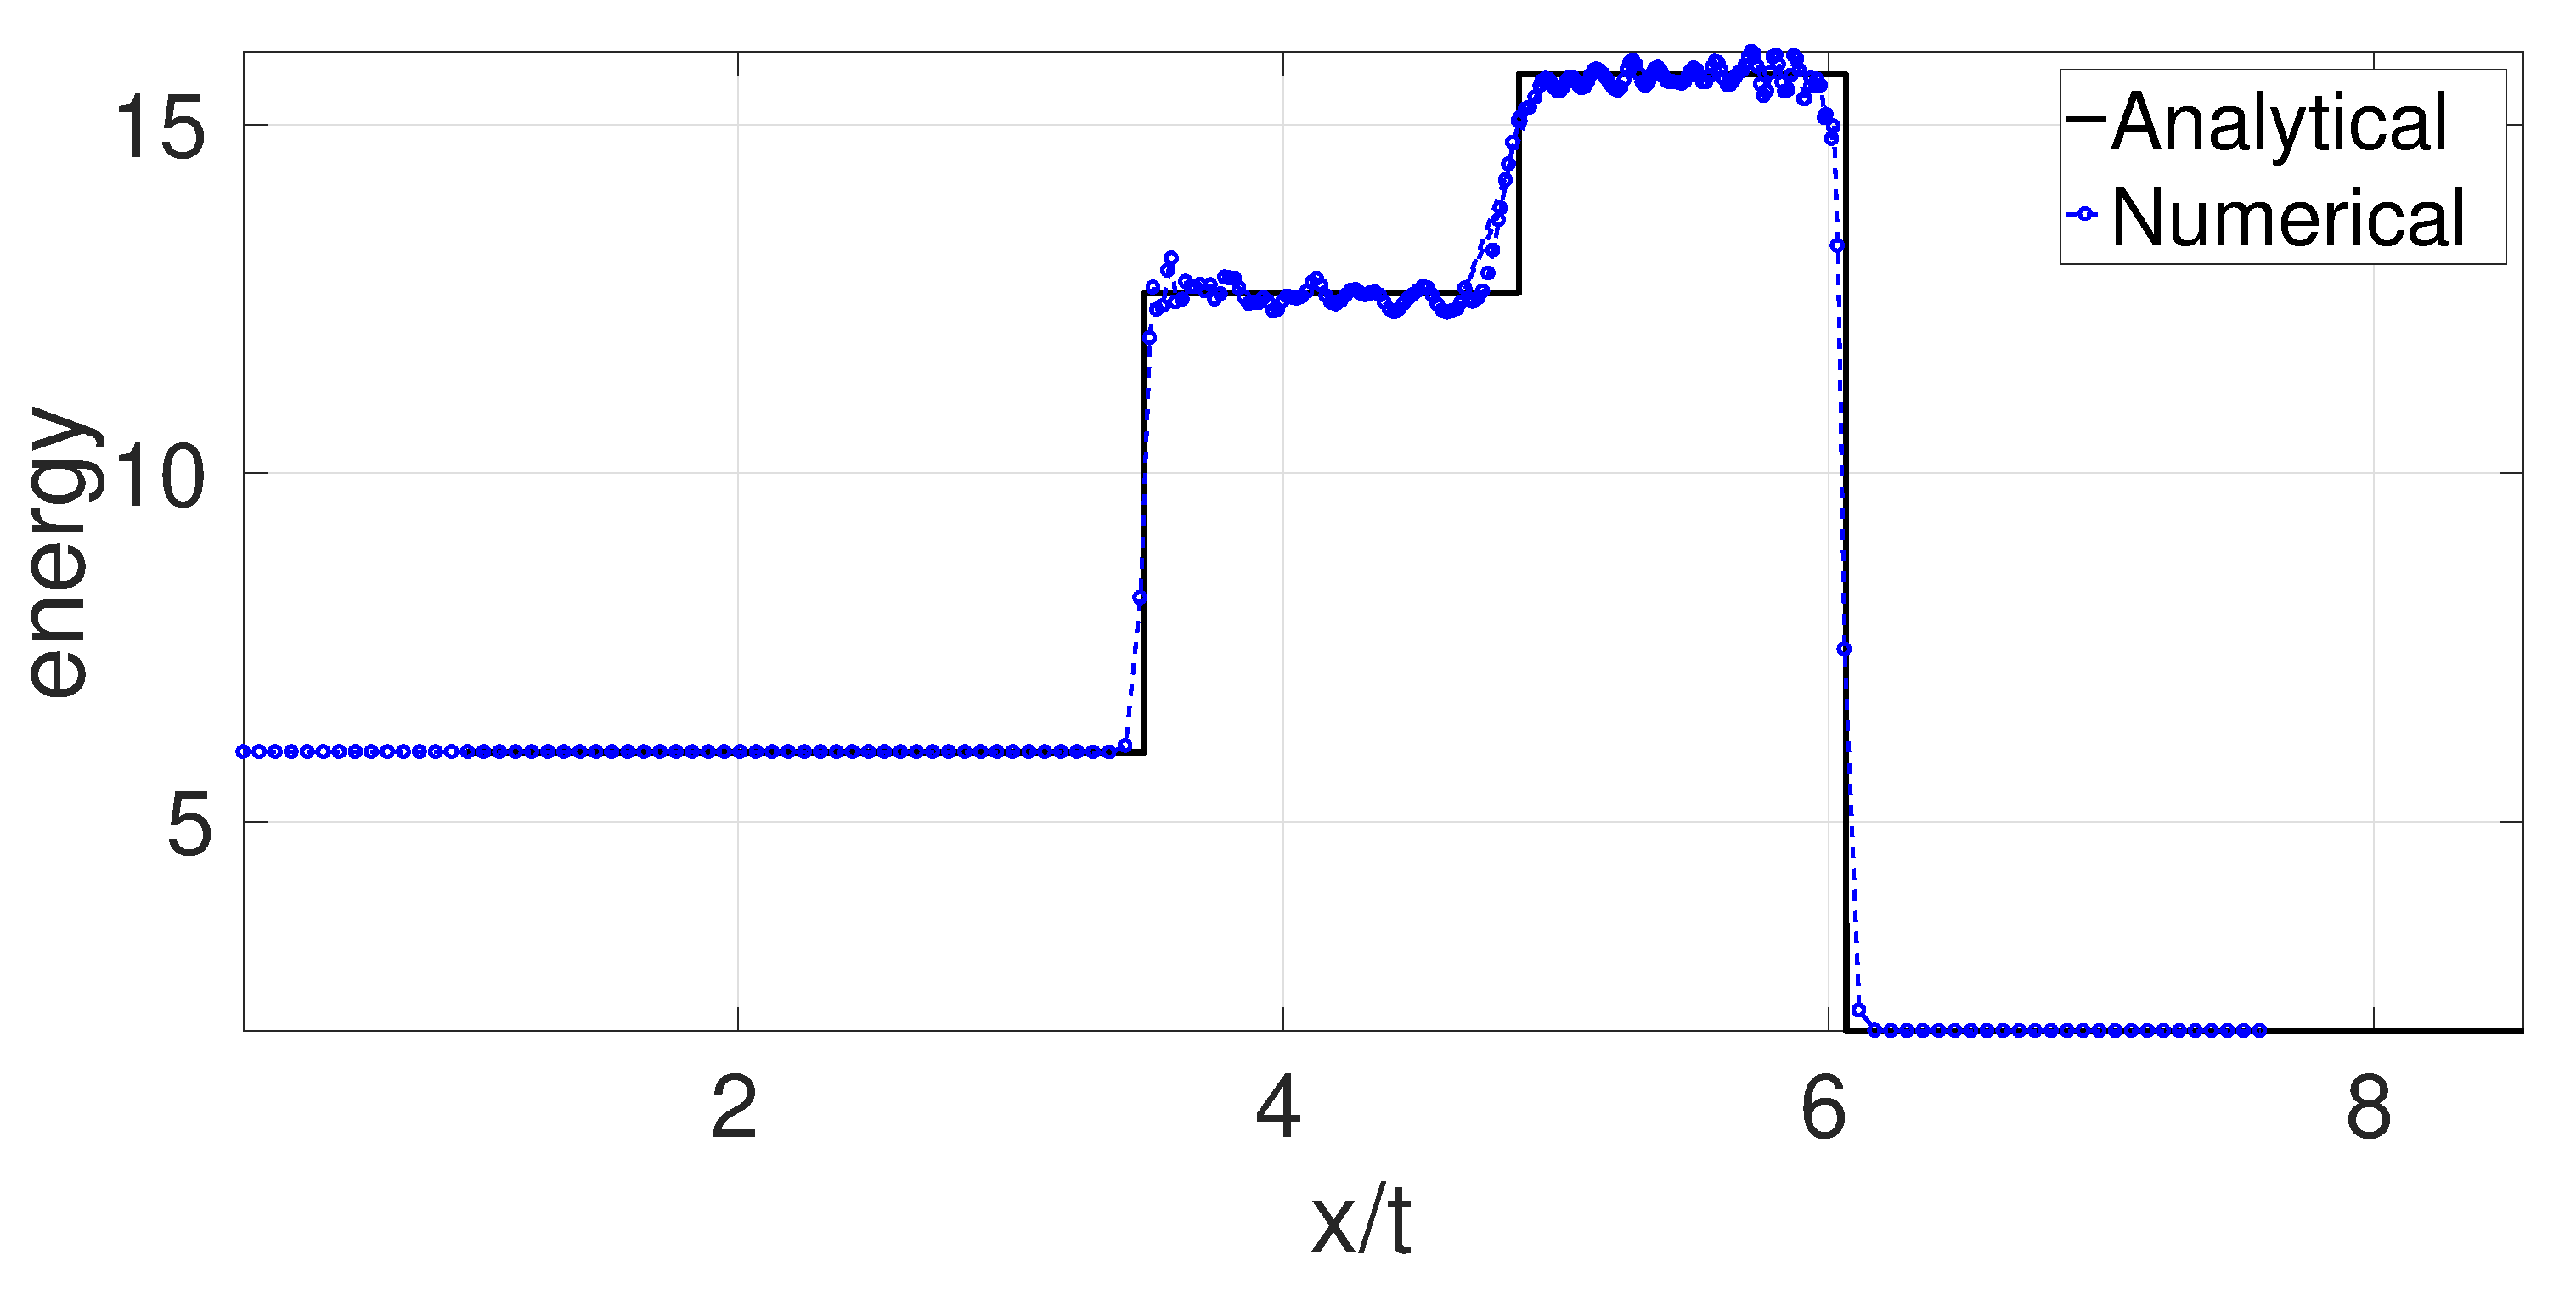
\includegraphics[width=0.99 \textwidth]{Chapter-4/Figures/double_shock/Dshock-RCM-e-Rp6}
    \end{minipage}%
    \begin{minipage}{.495 \textwidth}
        \centering
        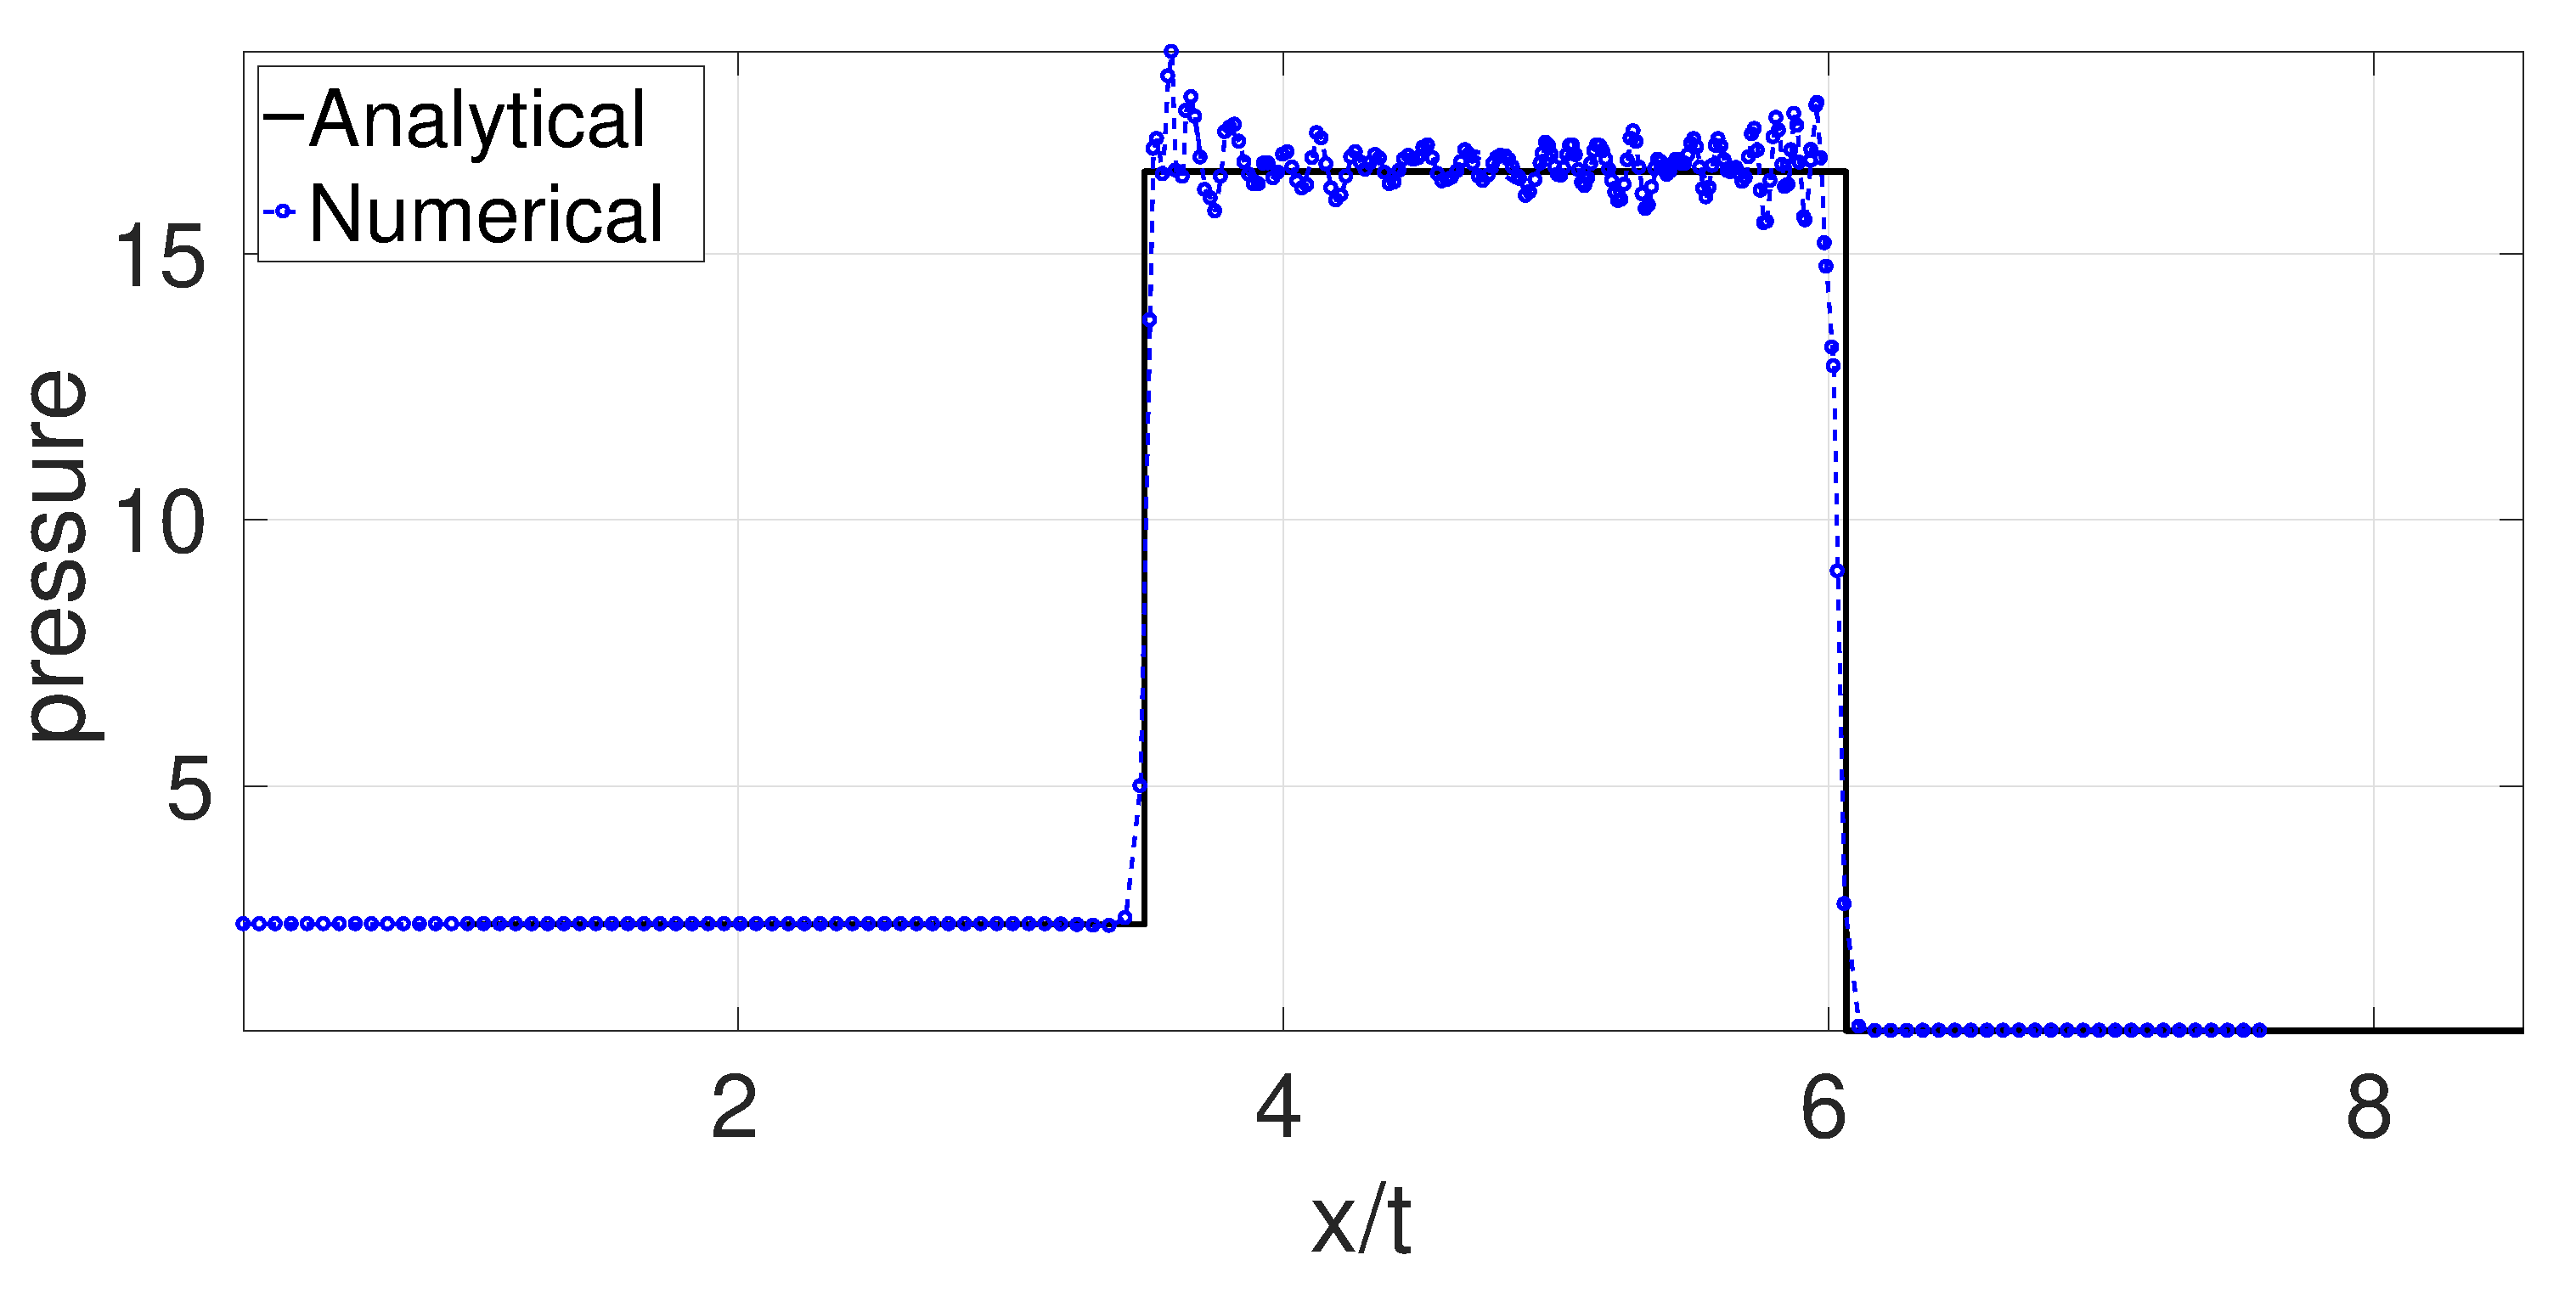
\includegraphics[width=0.99 \textwidth]{Chapter-4/Figures/double_shock/Dshock-RCM-p-Rp6}
    \end{minipage}% 
    \caption{Results for test 4, the double shock case. All physical properties are well re-produced. However, the oscillations are more serious than oscillations in other tests.}
    \label{fig:RCM-double-shock}
\end{figure}

\begin{figure}[H]
    %\centering
    \begin{minipage}{.495\textwidth}
        \centering
        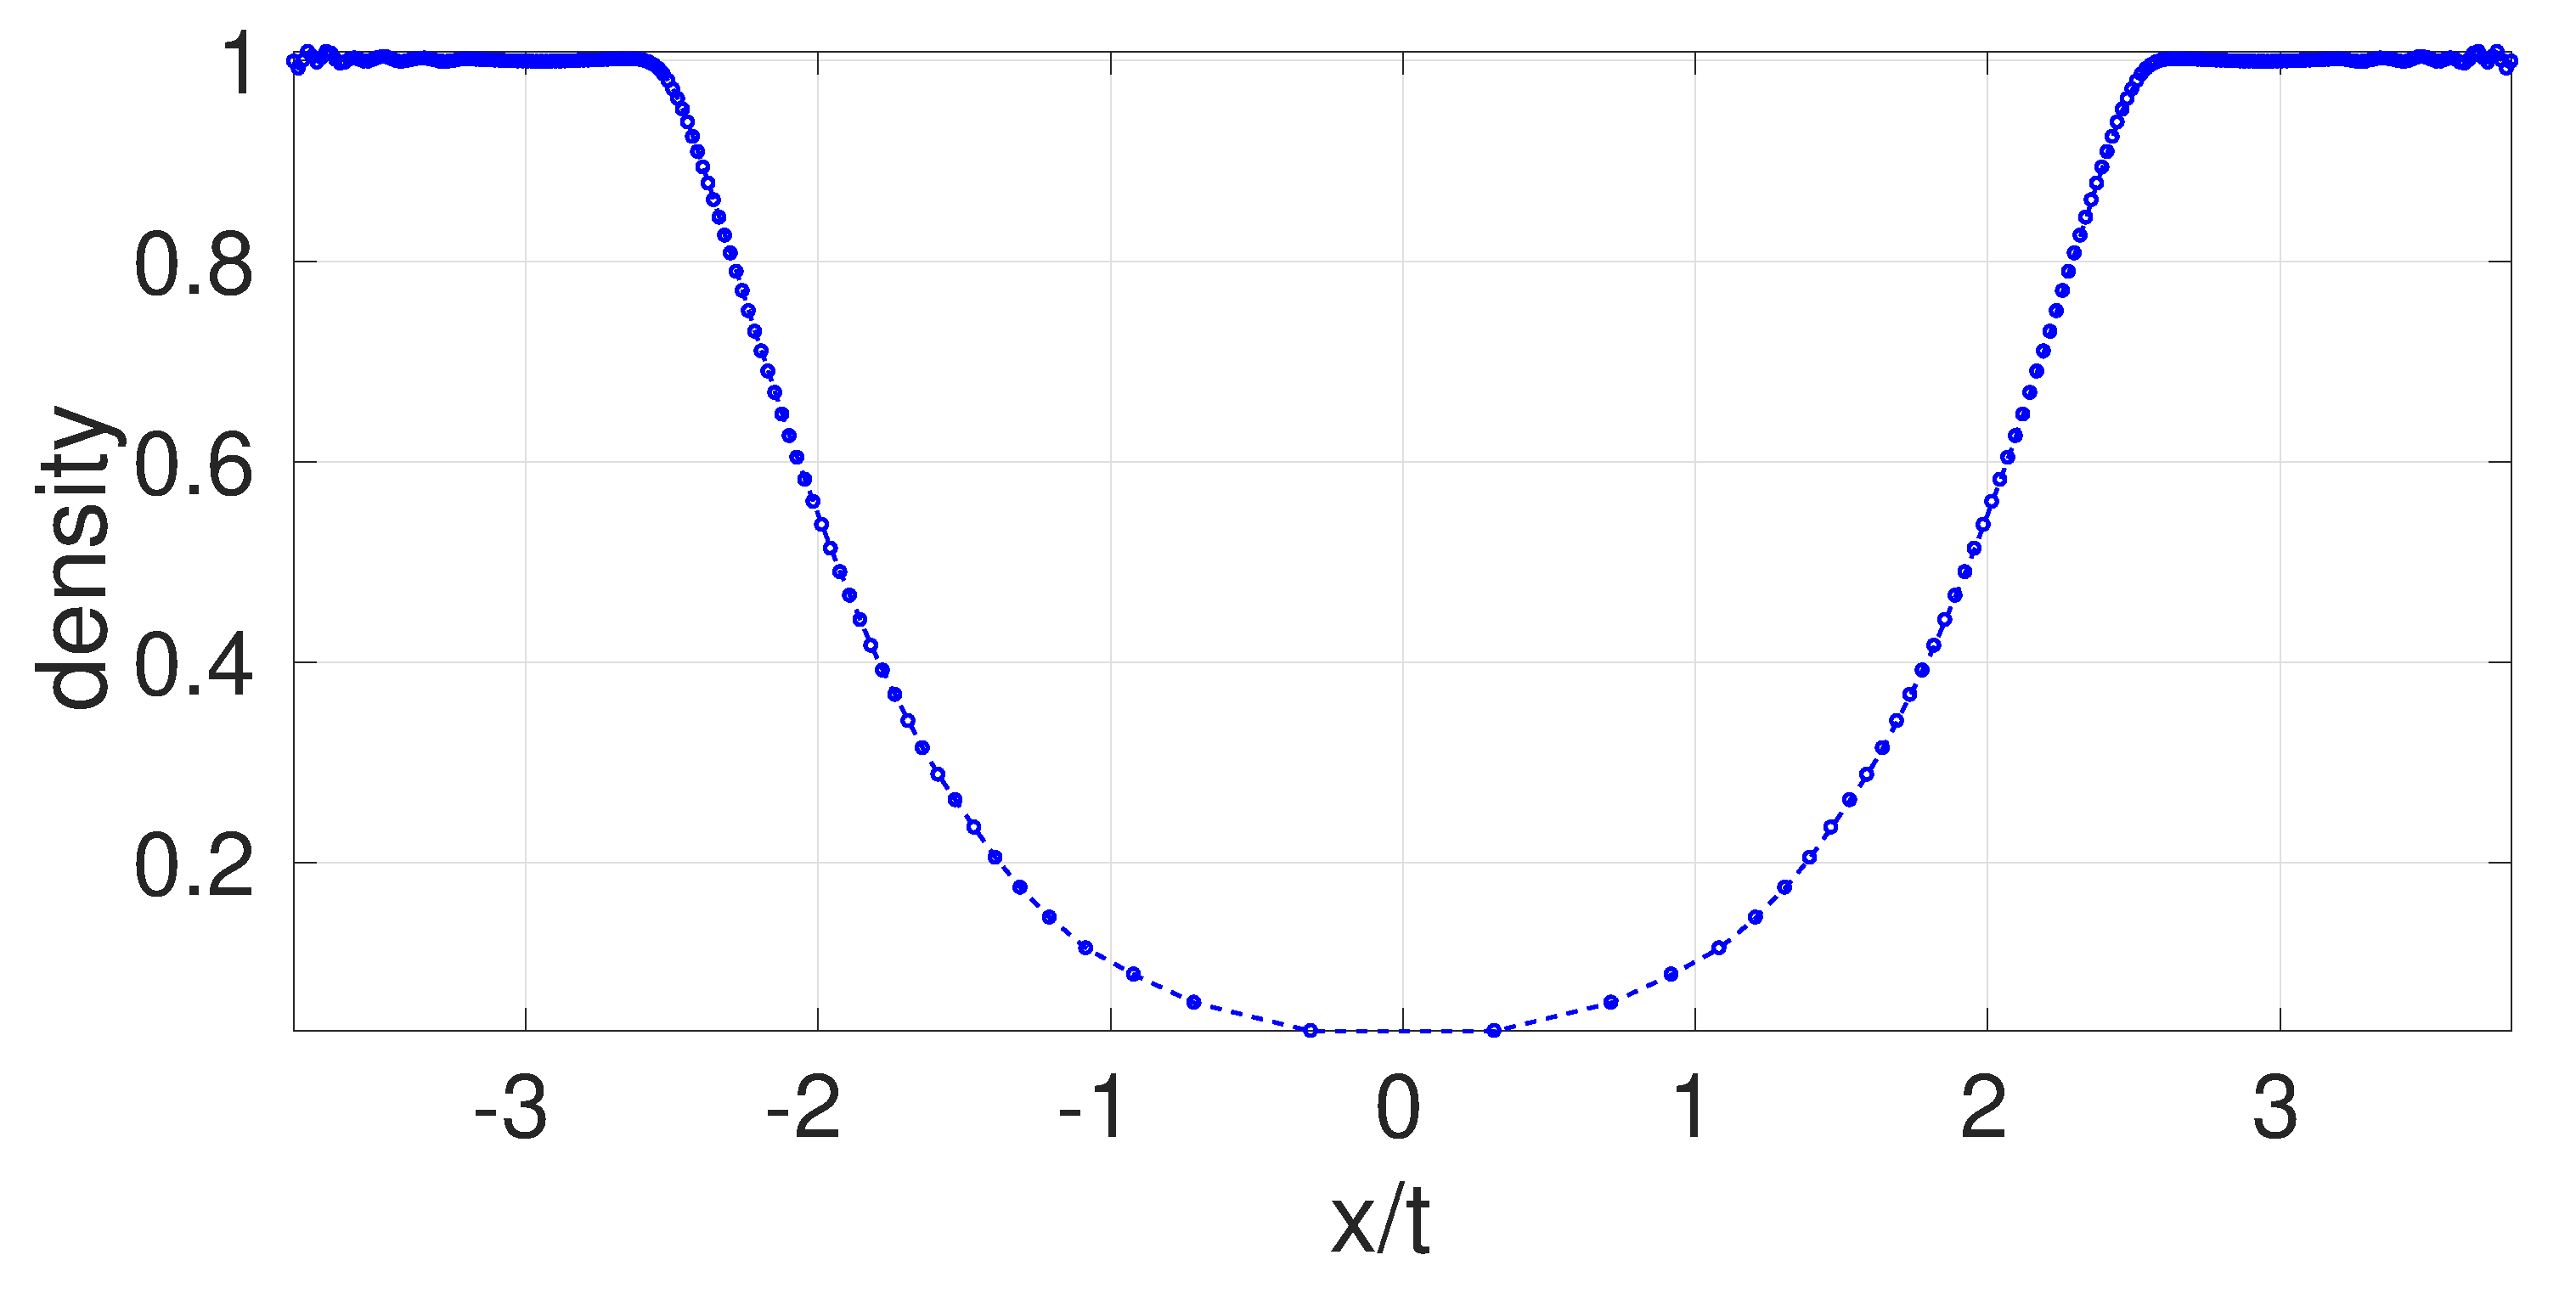
\includegraphics[width=0.99 \textwidth]{Chapter-4/Figures/Sjogreen/Sjogreen-RCM-rho-Adpt1}
    \end{minipage}%
    \begin{minipage}{.495 \textwidth}
        \centering
        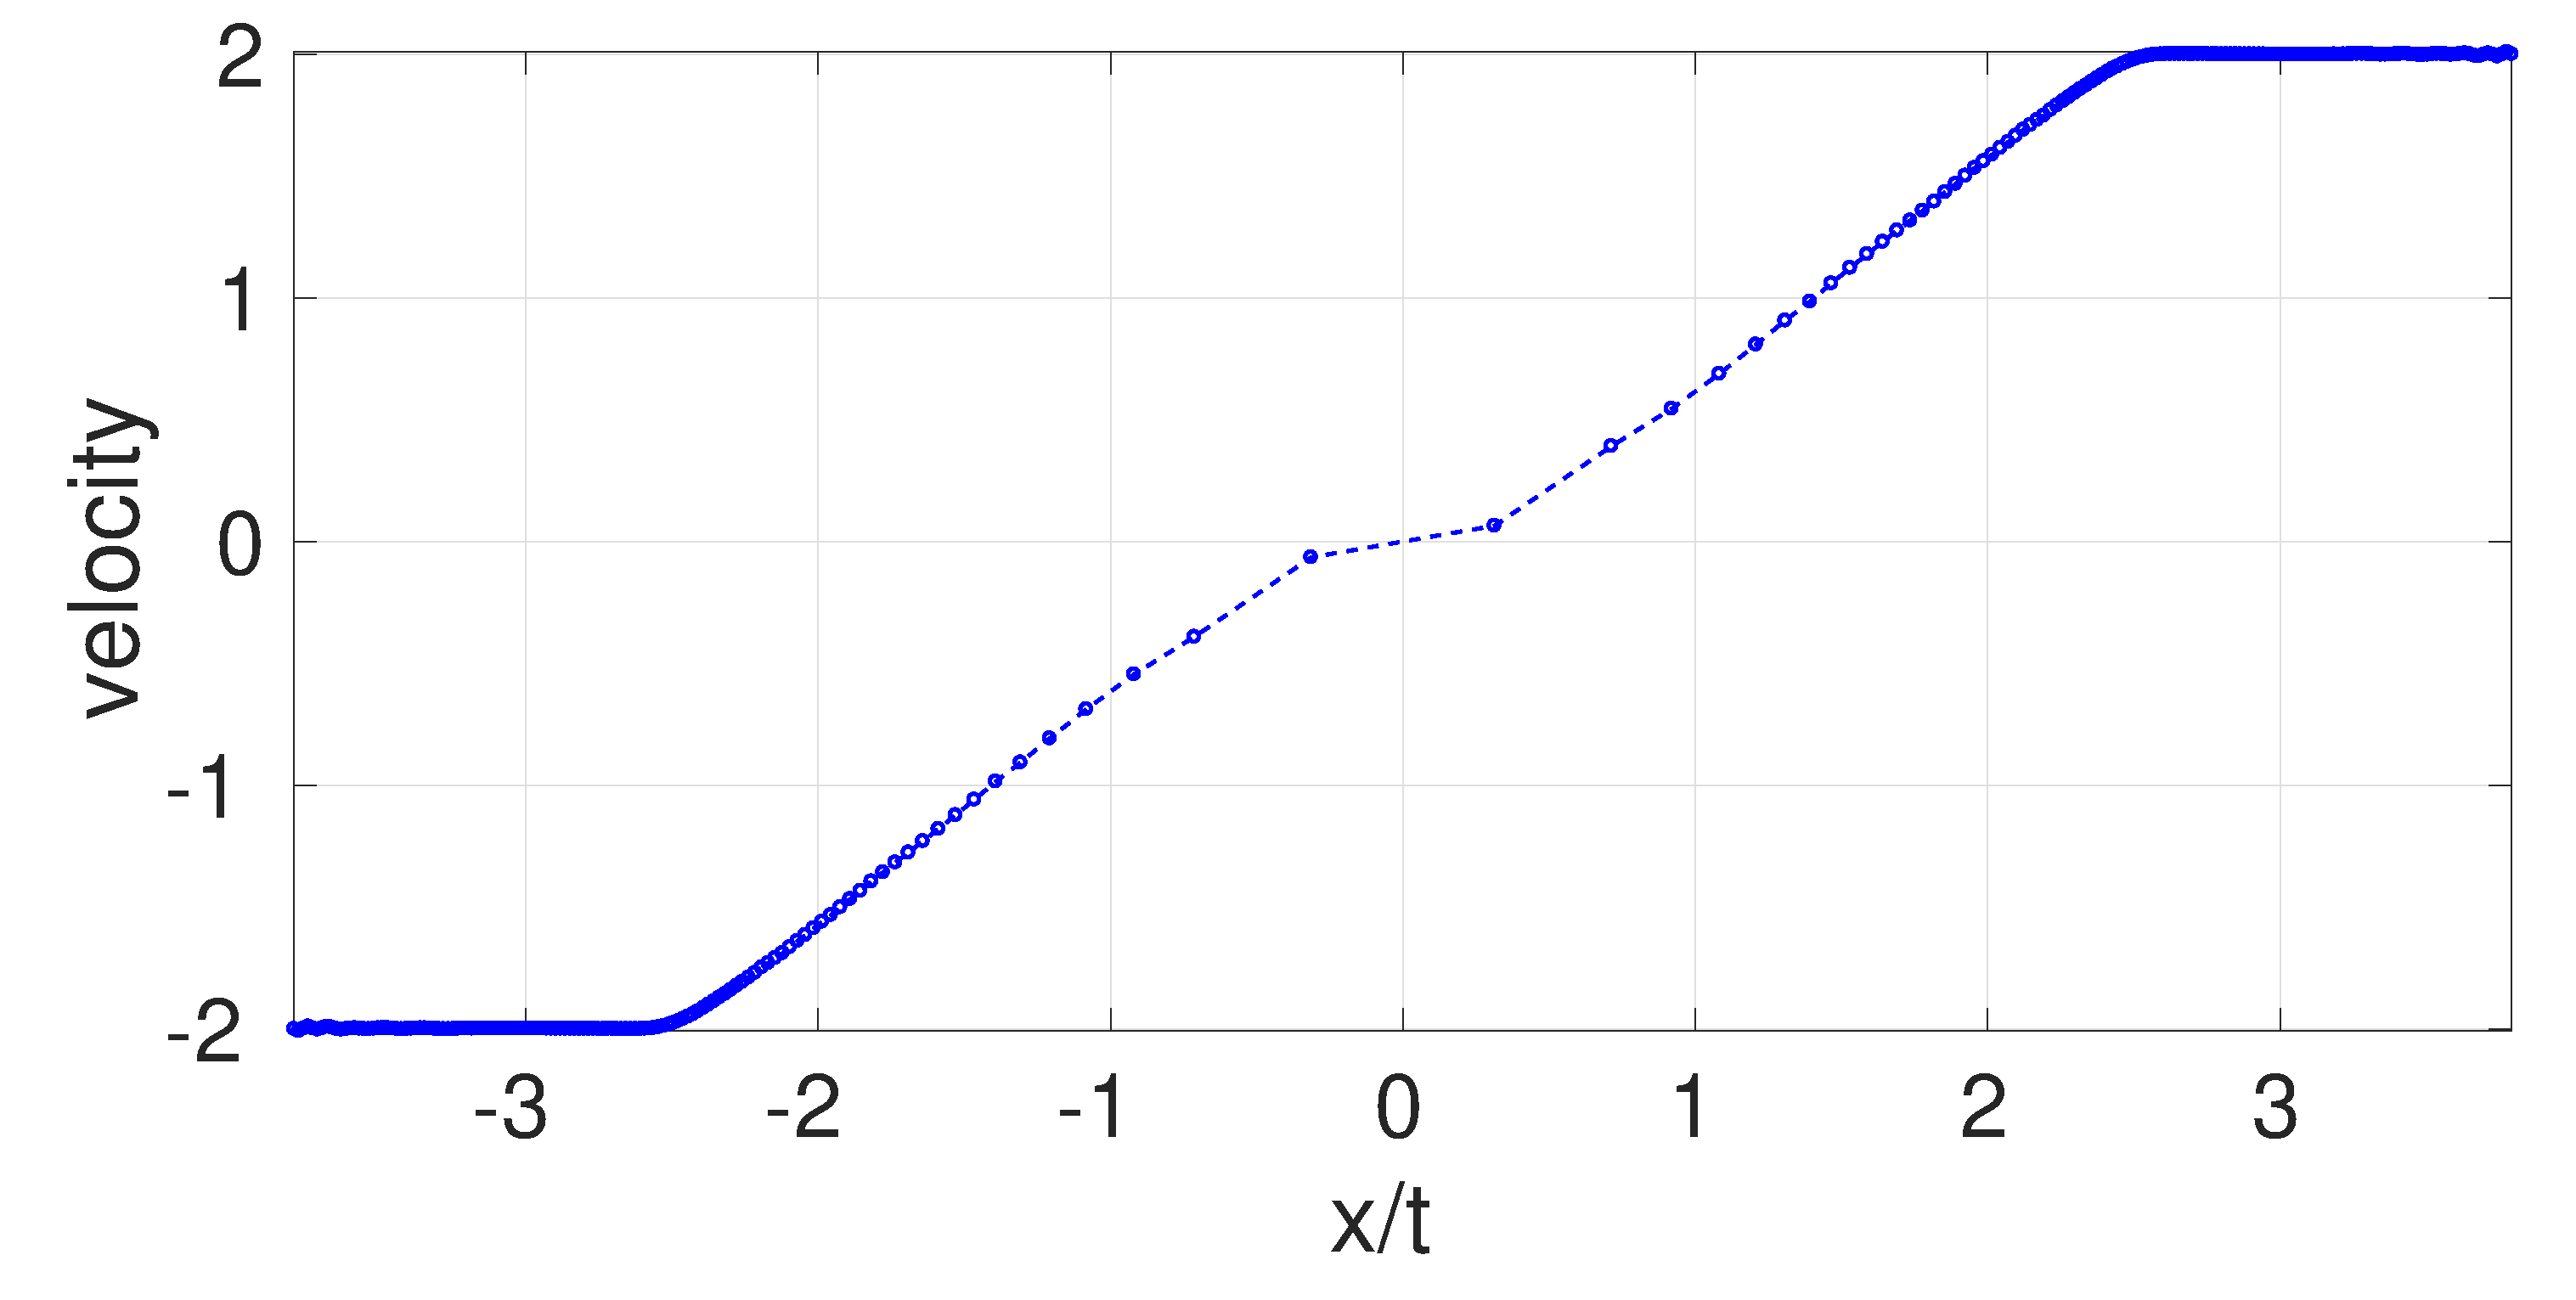
\includegraphics[width=0.99 \textwidth]{Chapter-4/Figures/Sjogreen/Sjogreen-RCM-v-Adpt1}
    \end{minipage}%
    \\
    \begin{minipage}{.495\textwidth}
        \centering
        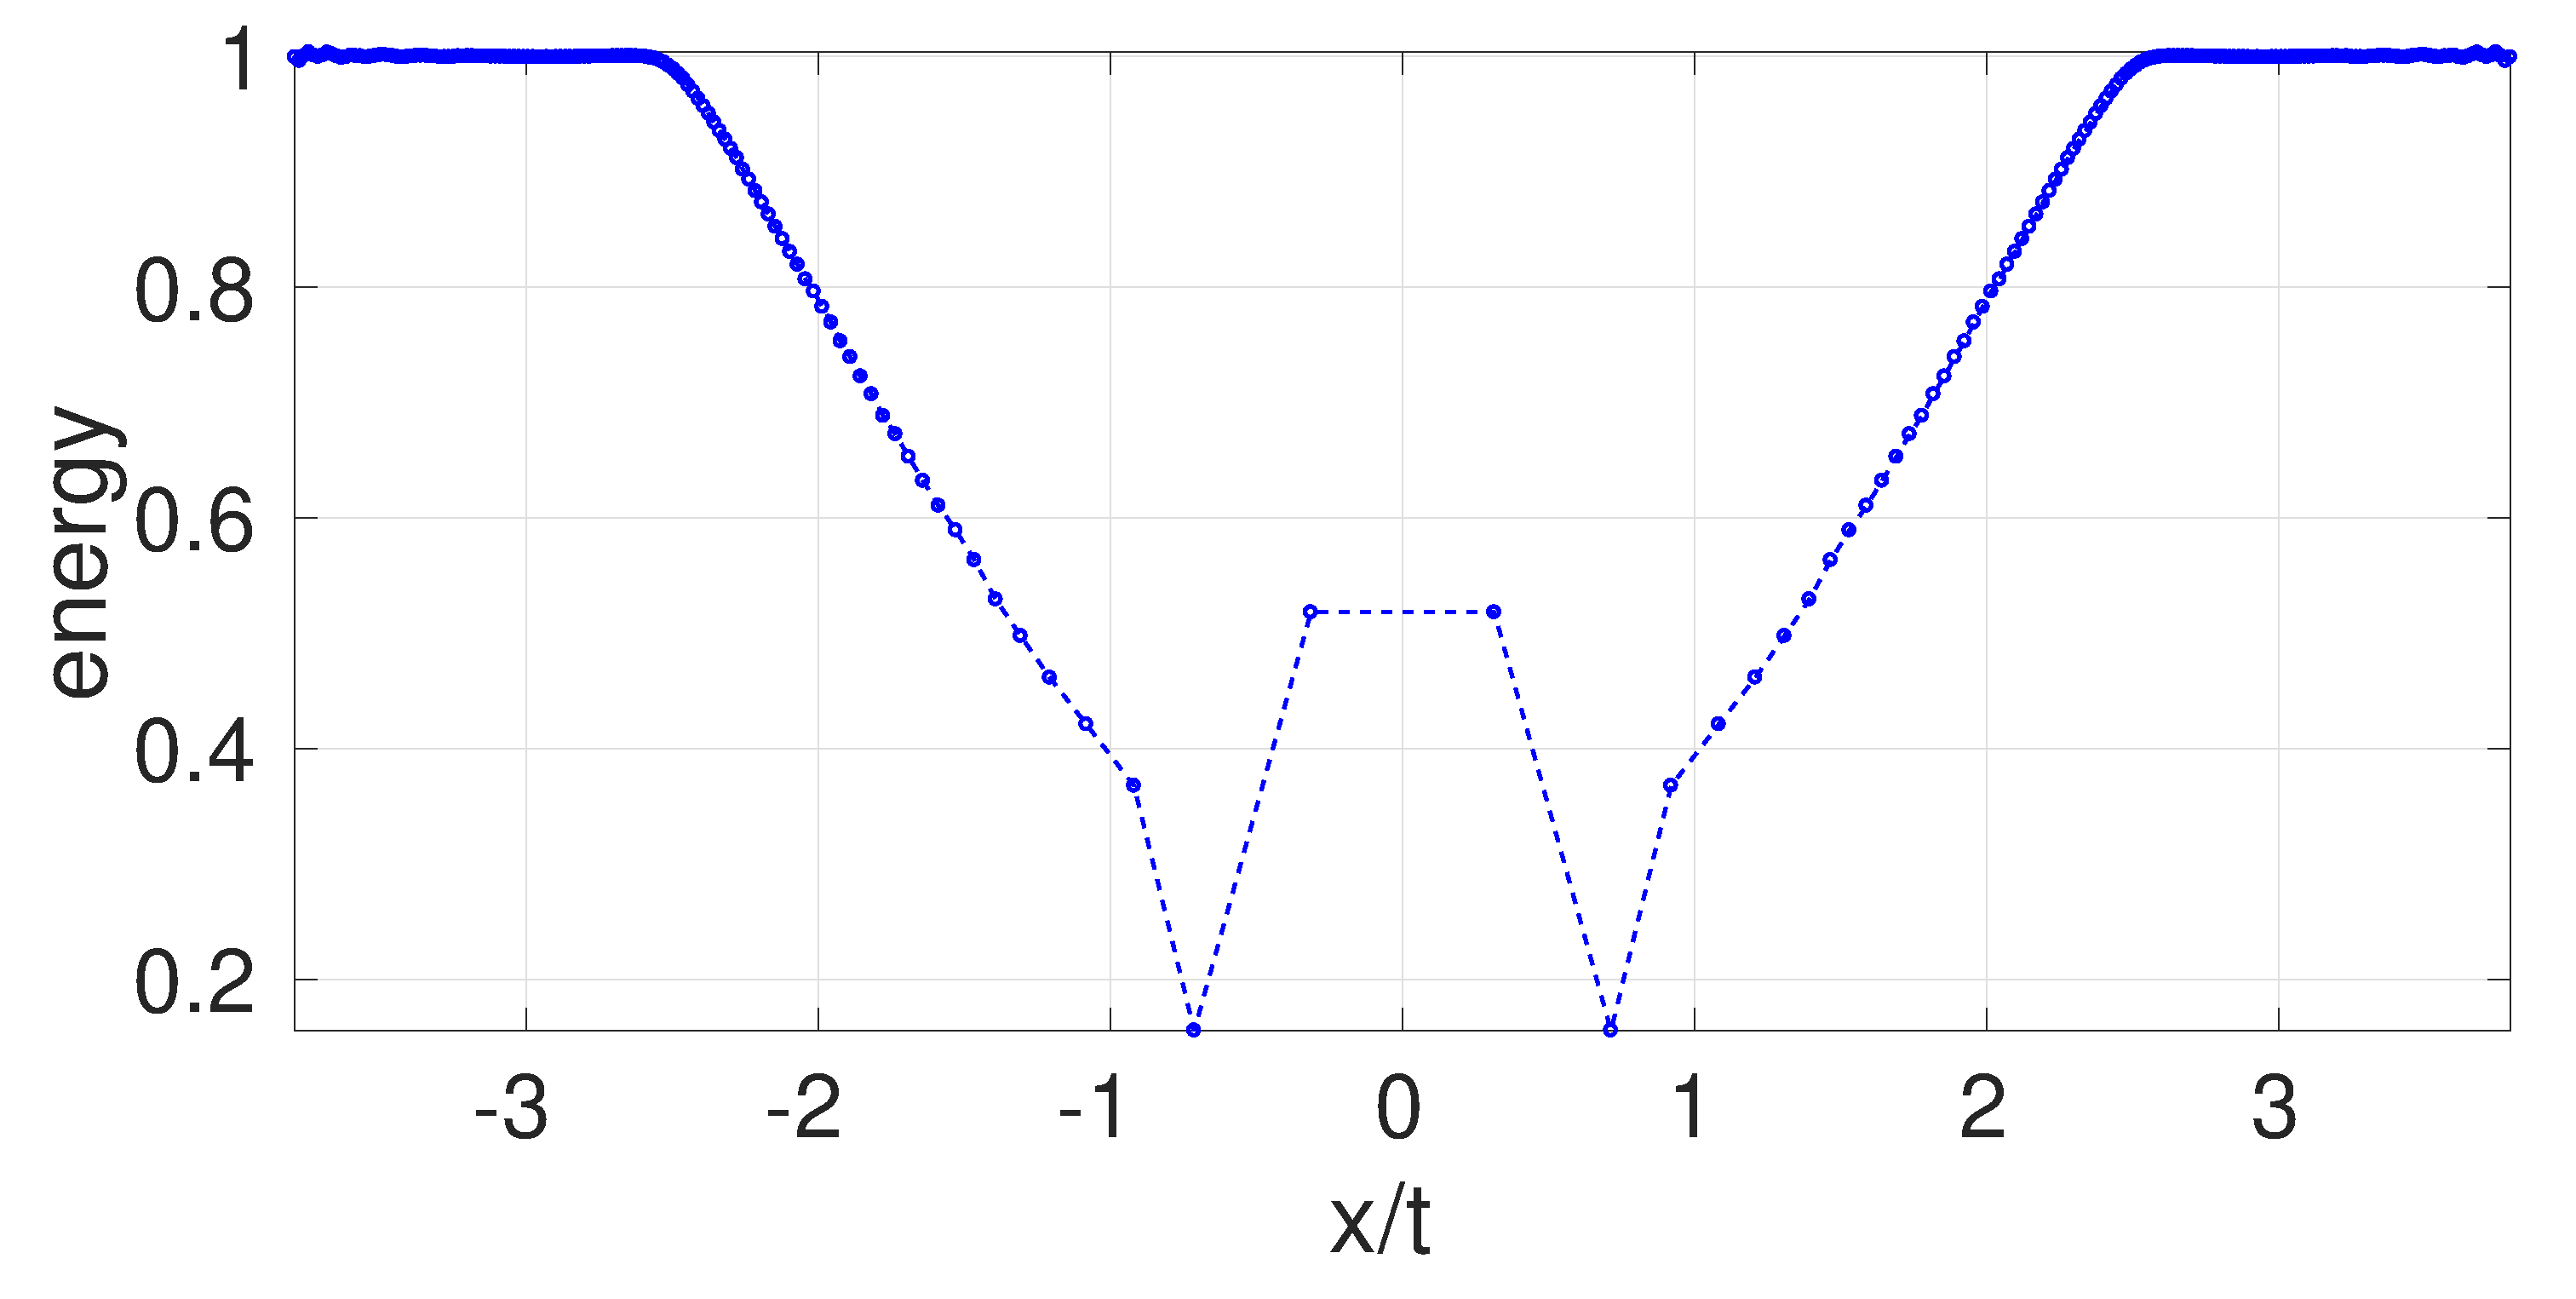
\includegraphics[width=0.99 \textwidth]{Chapter-4/Figures/Sjogreen/Sjogreen-RCM-e-Adpt1}
    \end{minipage}%
    \begin{minipage}{.495 \textwidth}
        \centering
        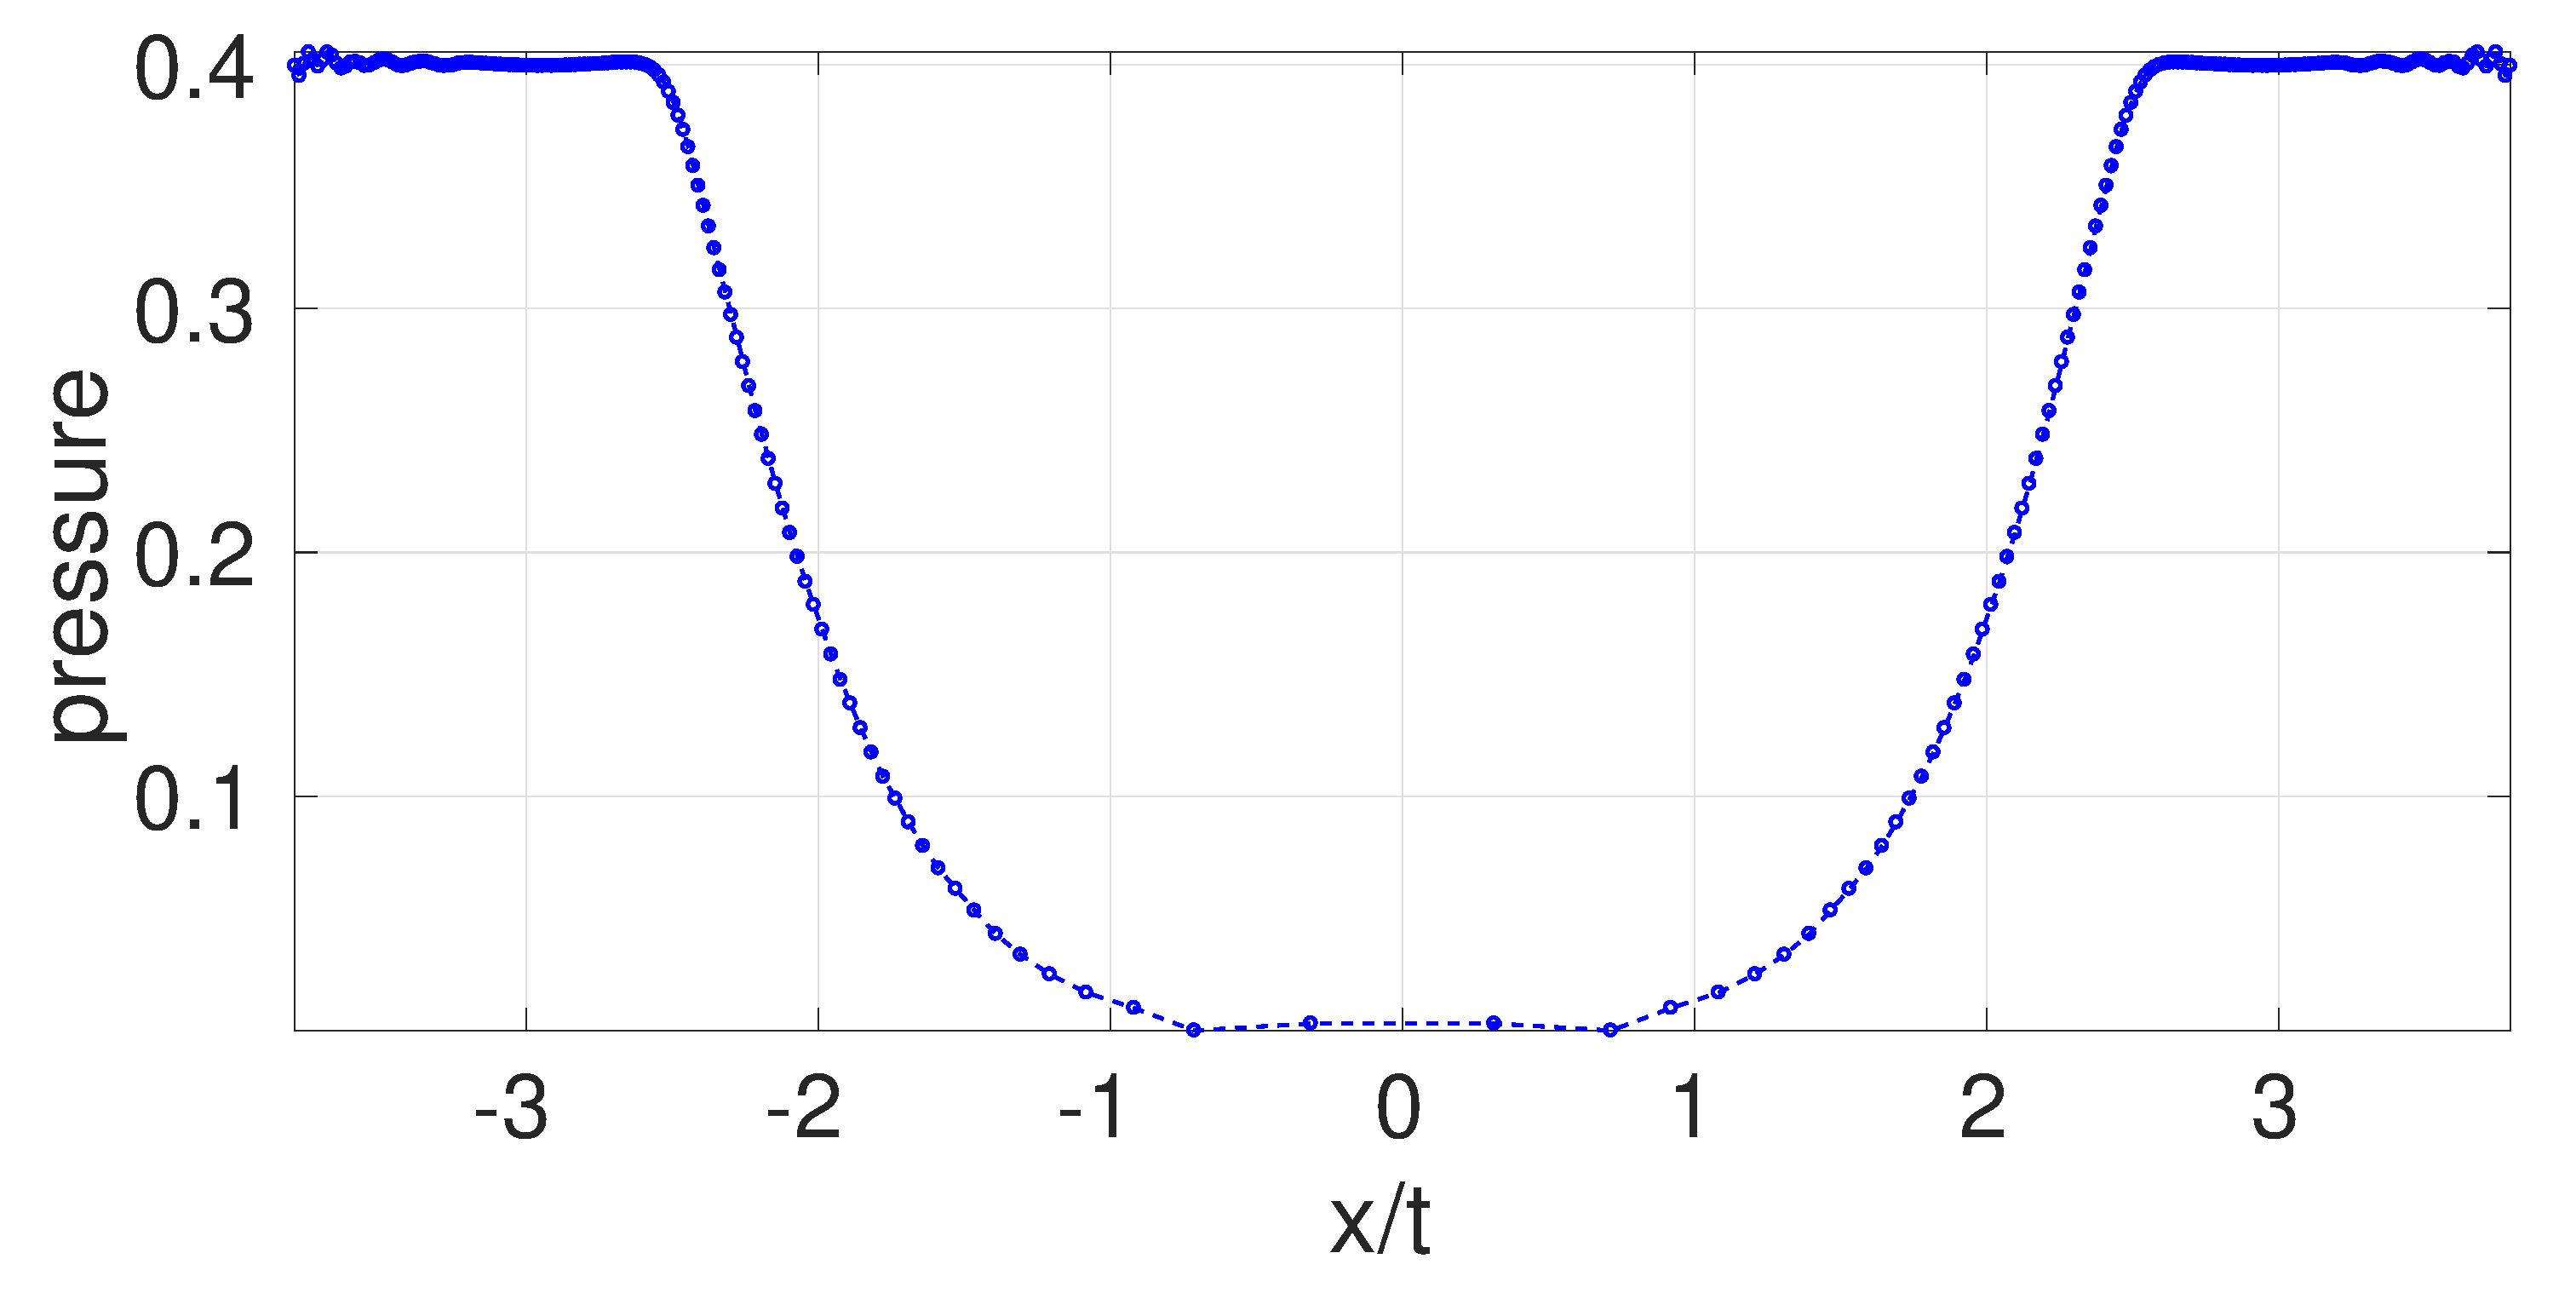
\includegraphics[width=0.99 \textwidth]{Chapter-4/Figures/Sjogreen/Sjogreen-RCM-p-Adpt1}
    \end{minipage}% 
    \caption{Results for test 5, a variation of the Sjogreen test. The density, velocity and pressure are well re-produced while the thermal energy at the origin is poorly predict. A jump of internal energy at the origin is a common issue in many SPH schemes (see, for example, \citep{monaghan1997sph,cha2003implementations,puri2014approximate})}
    \label{fig:RCM-Sjogreen}
\end{figure}

\begin{figure}[H]
    \centering
    \begin{minipage}{.495\textwidth}
        \centering
        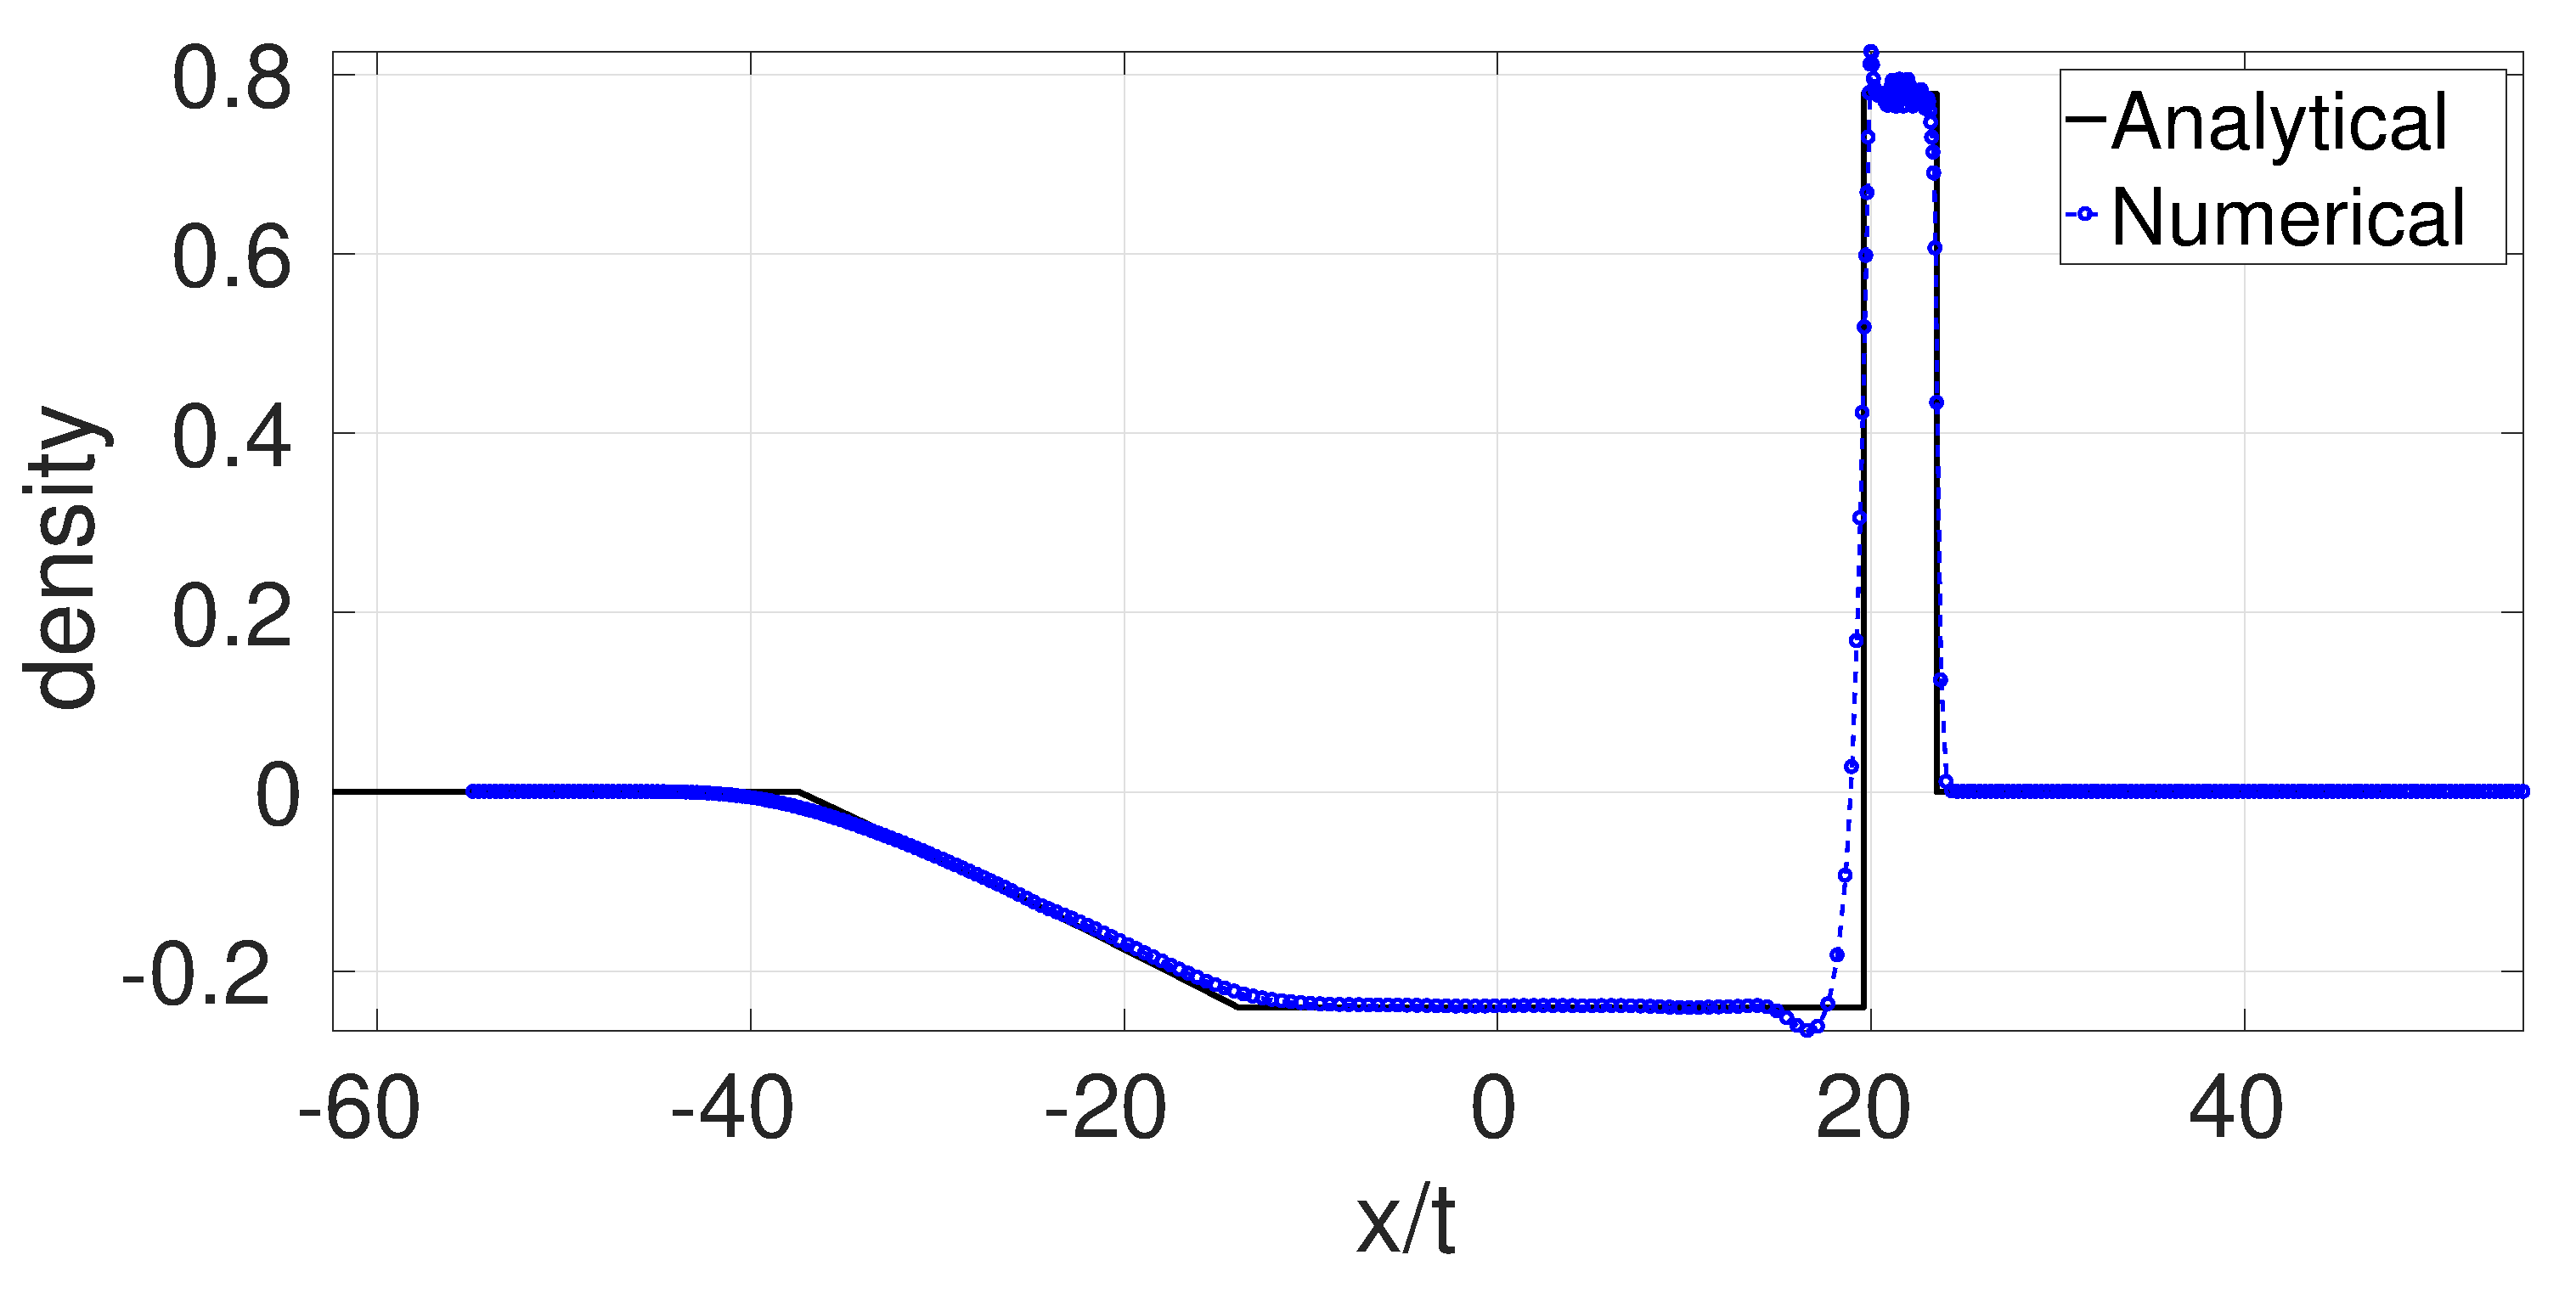
\includegraphics[width=0.99 \textwidth]{Chapter-4/Figures/strong-blast/StrBlst-RCM-rho-Rp3}
    \end{minipage}%
    \begin{minipage}{.495 \textwidth}
        \centering
        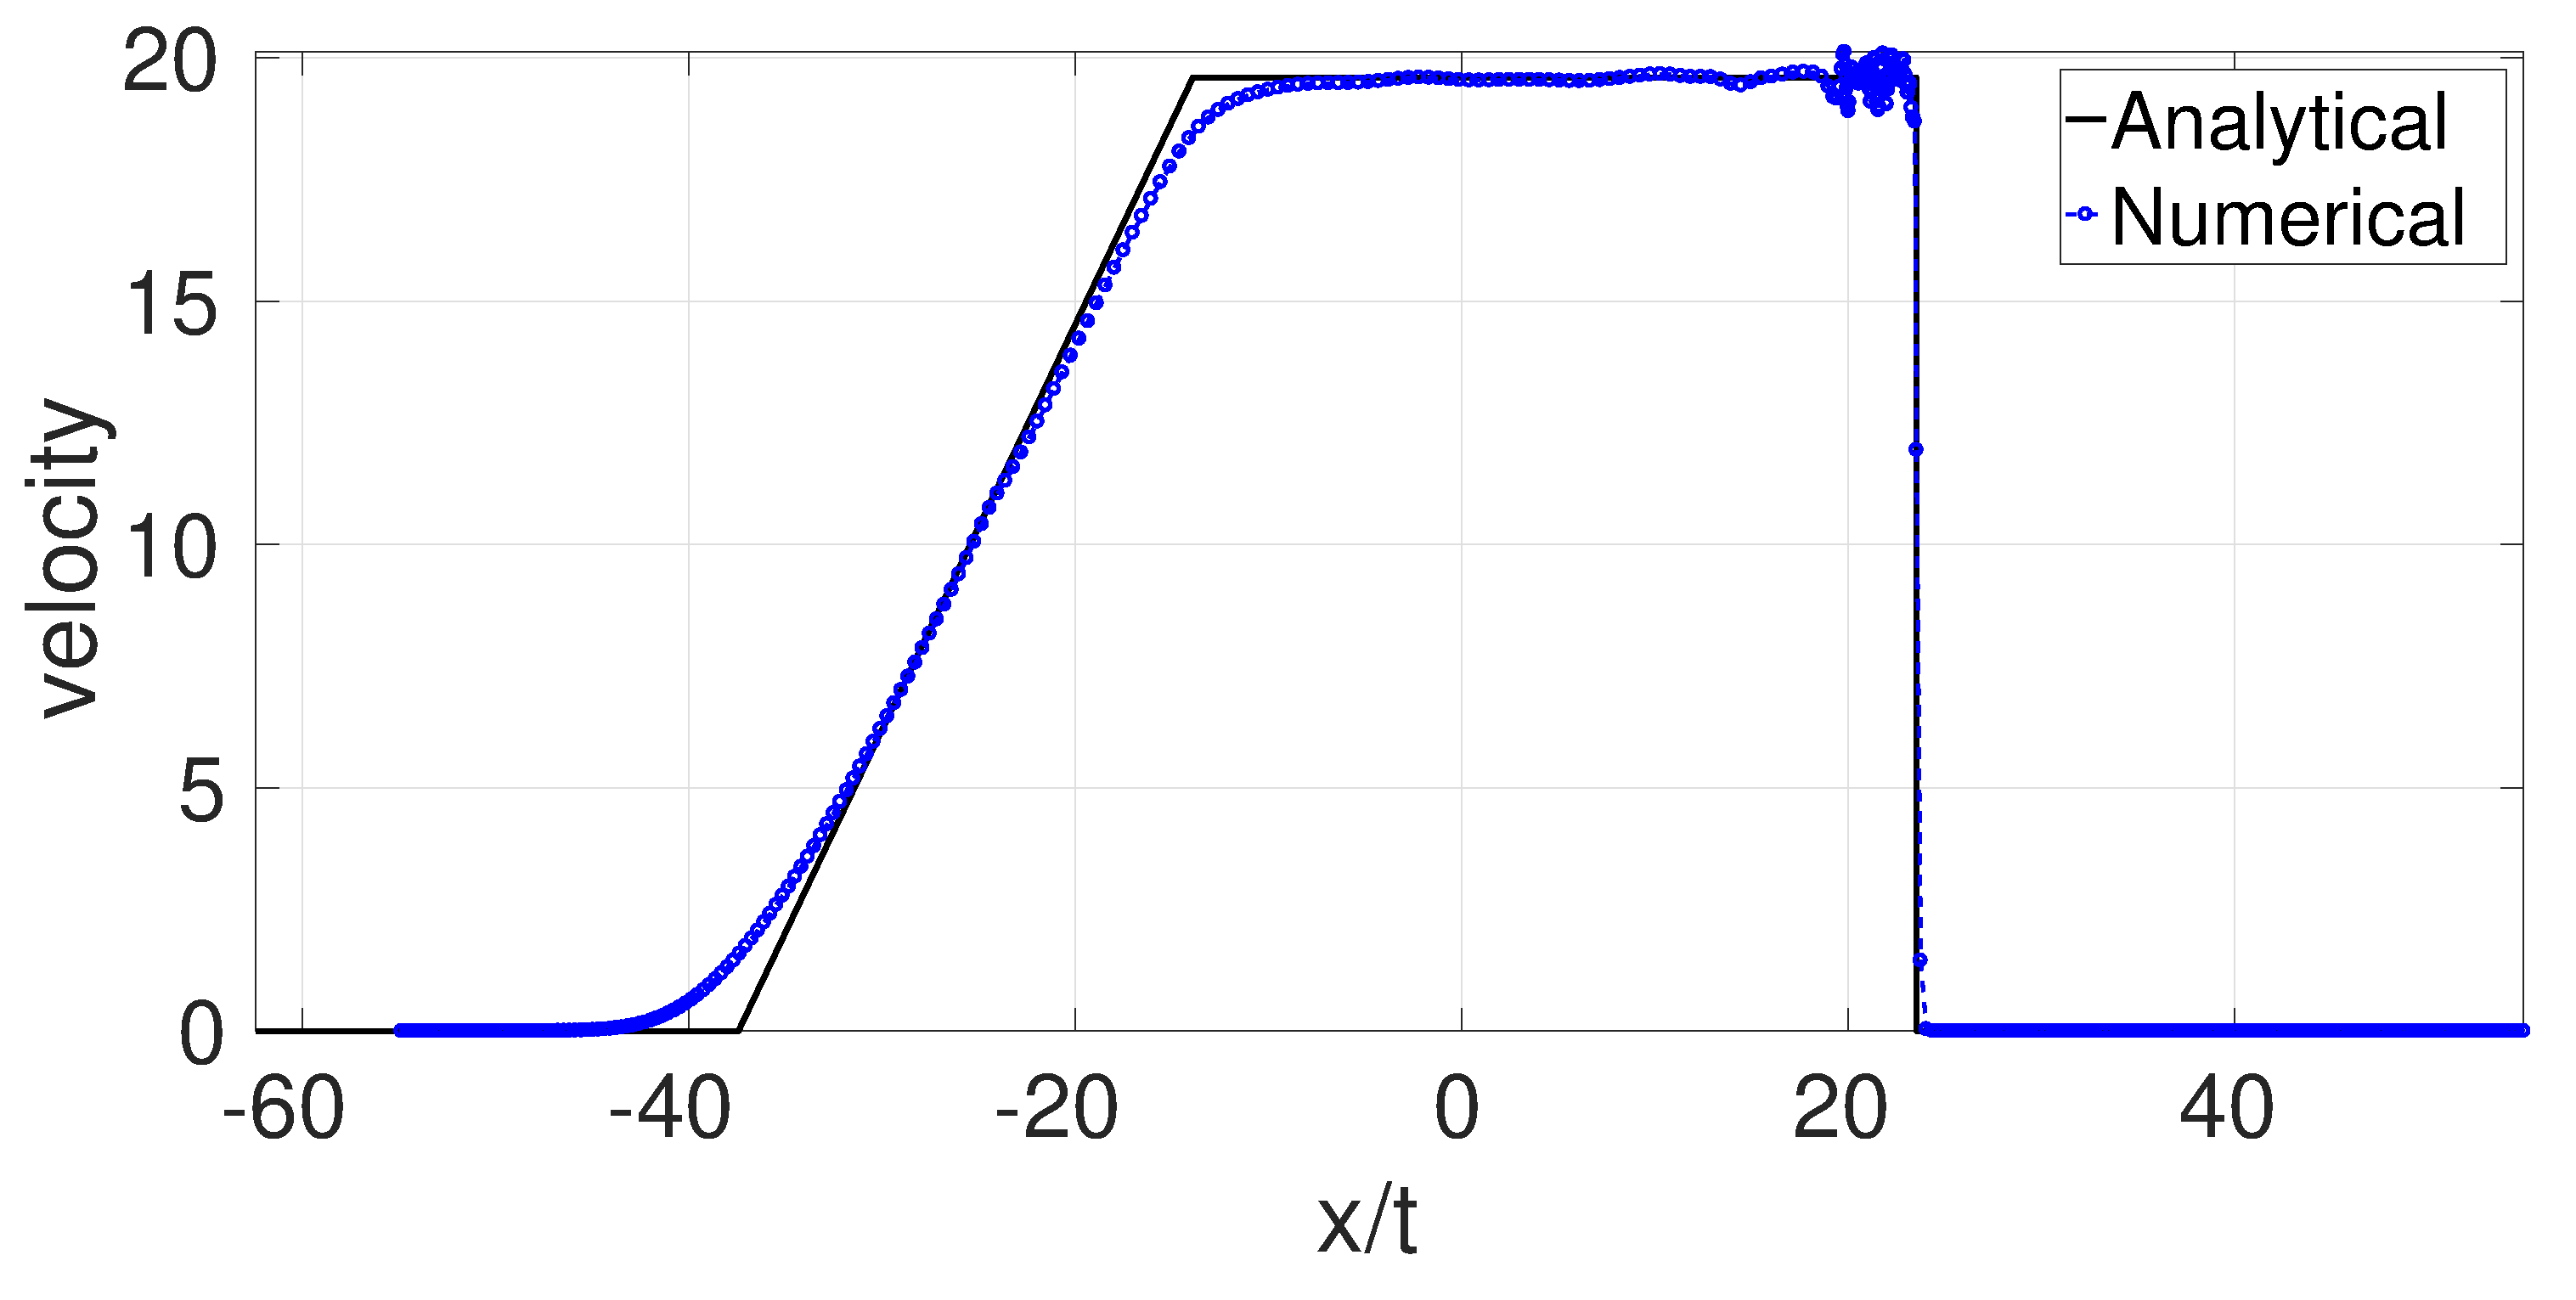
\includegraphics[width=0.99 \textwidth]{Chapter-4/Figures/strong-blast/StrBlst-RCM-v-Rp3}
    \end{minipage}%
    \\
    \begin{minipage}{.495 \textwidth}
        \centering
        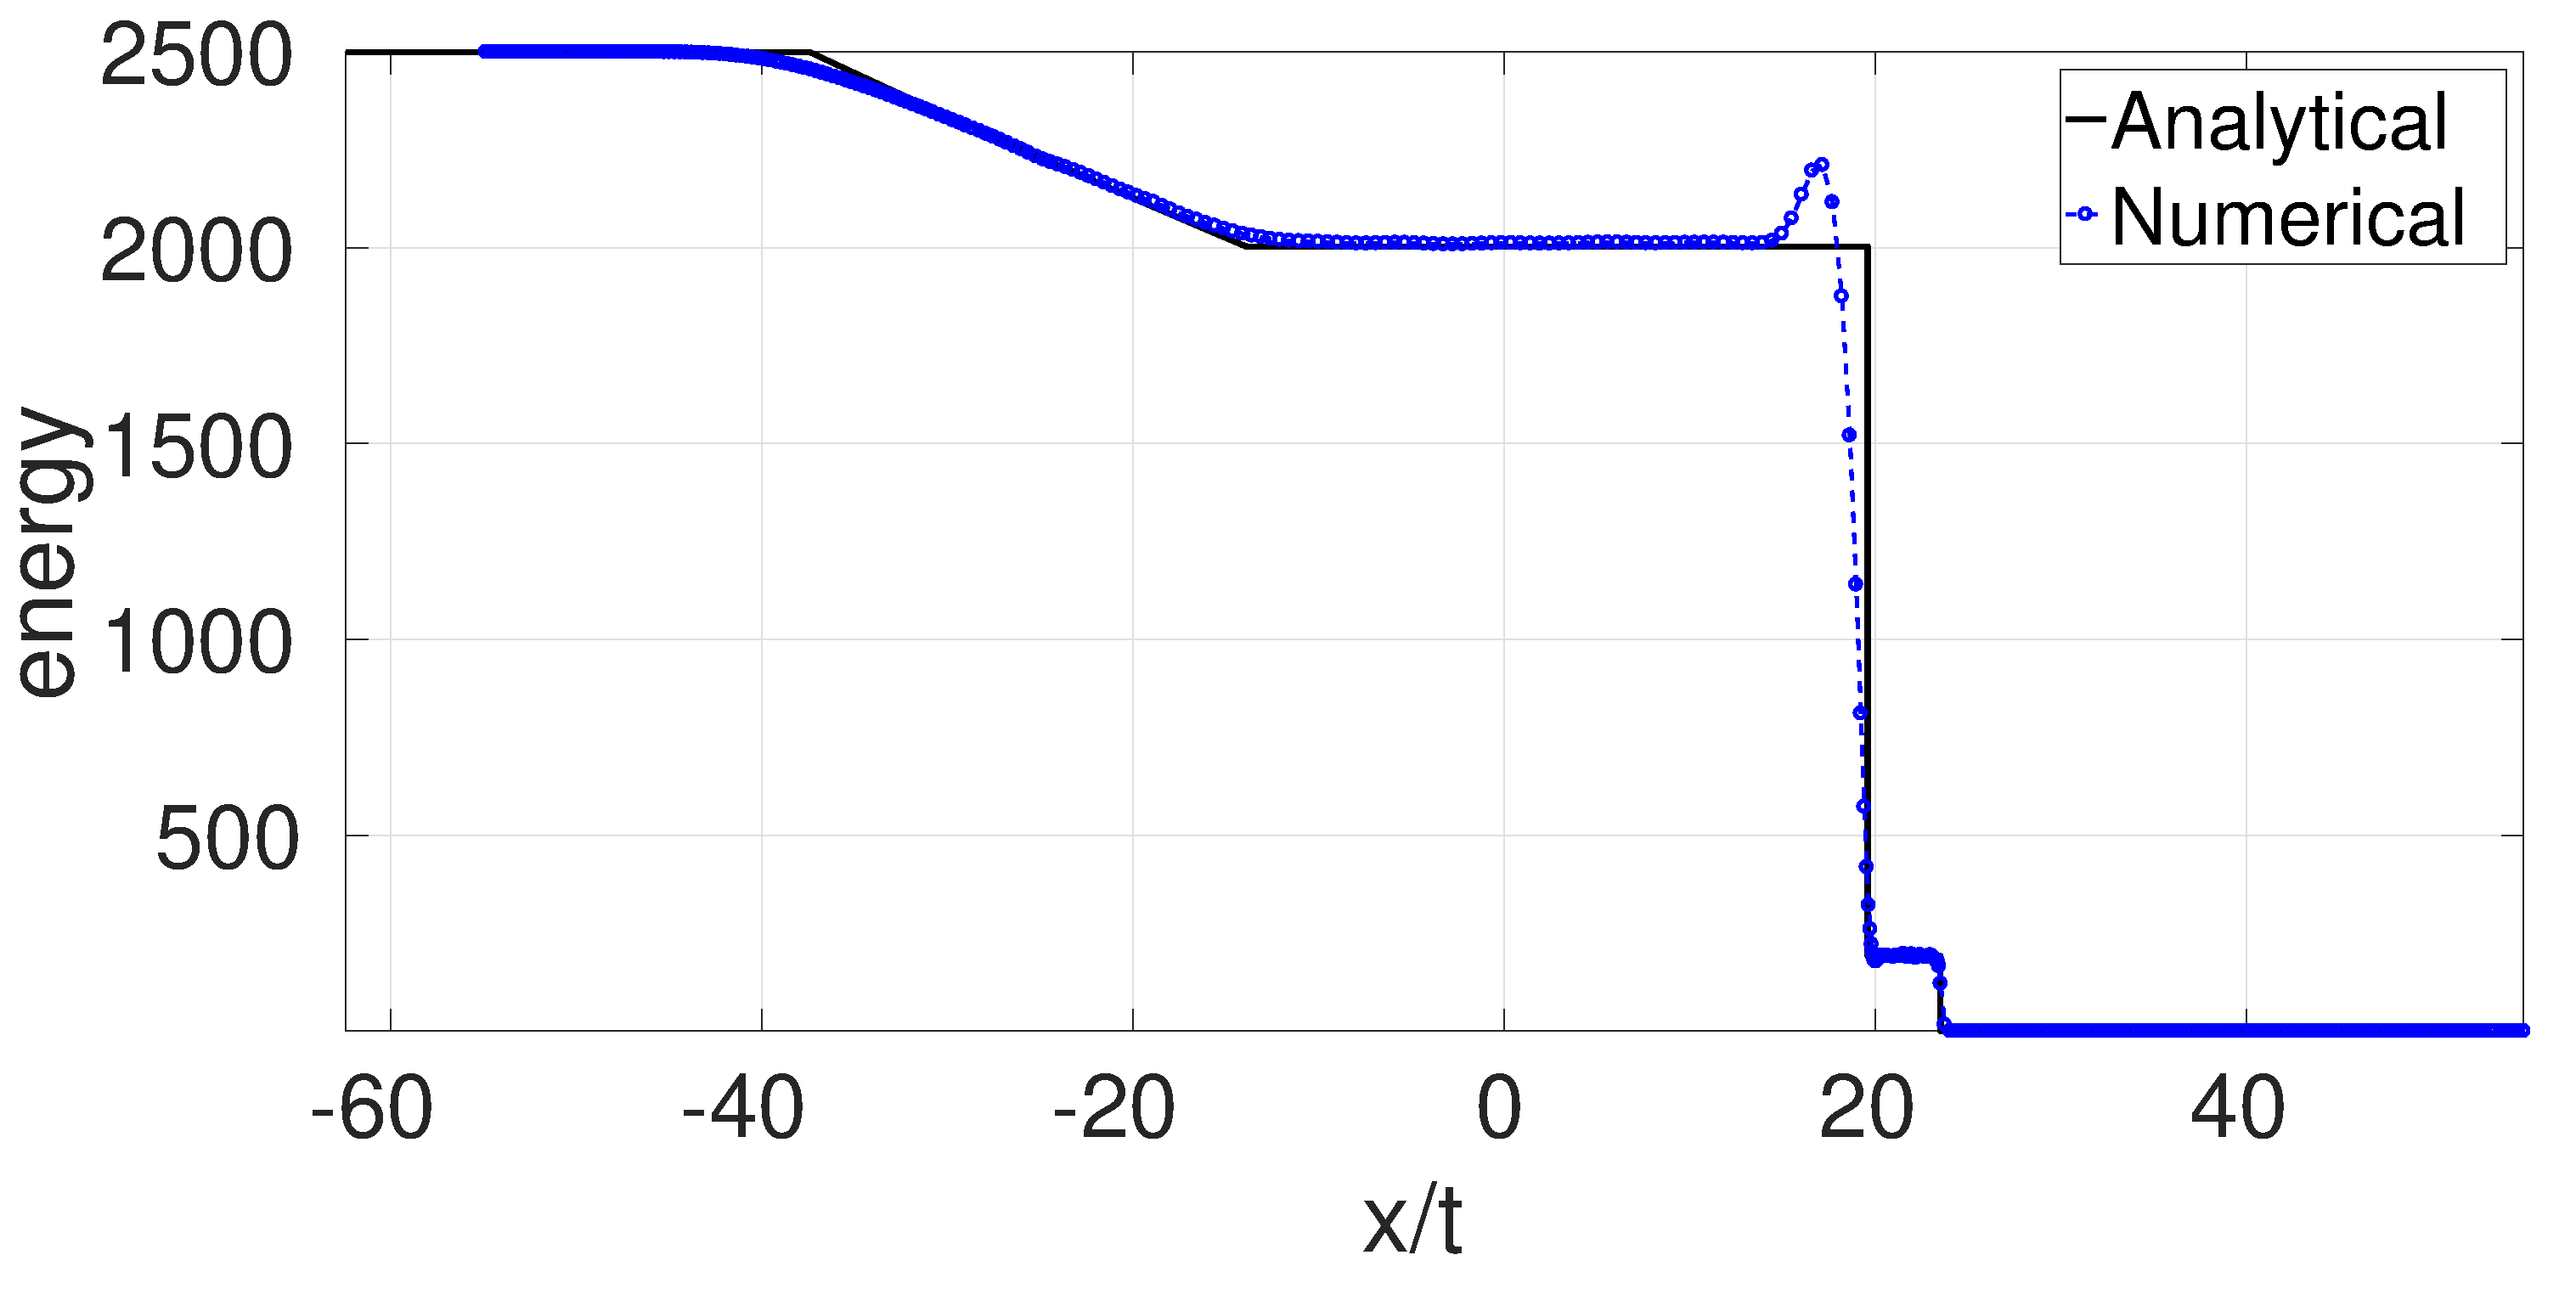
\includegraphics[width=0.99 \textwidth]{Chapter-4/Figures/strong-blast/StrBlst-RCM-e-Rp3}
    \end{minipage}%
    \begin{minipage}{.495 \textwidth}
        \centering
        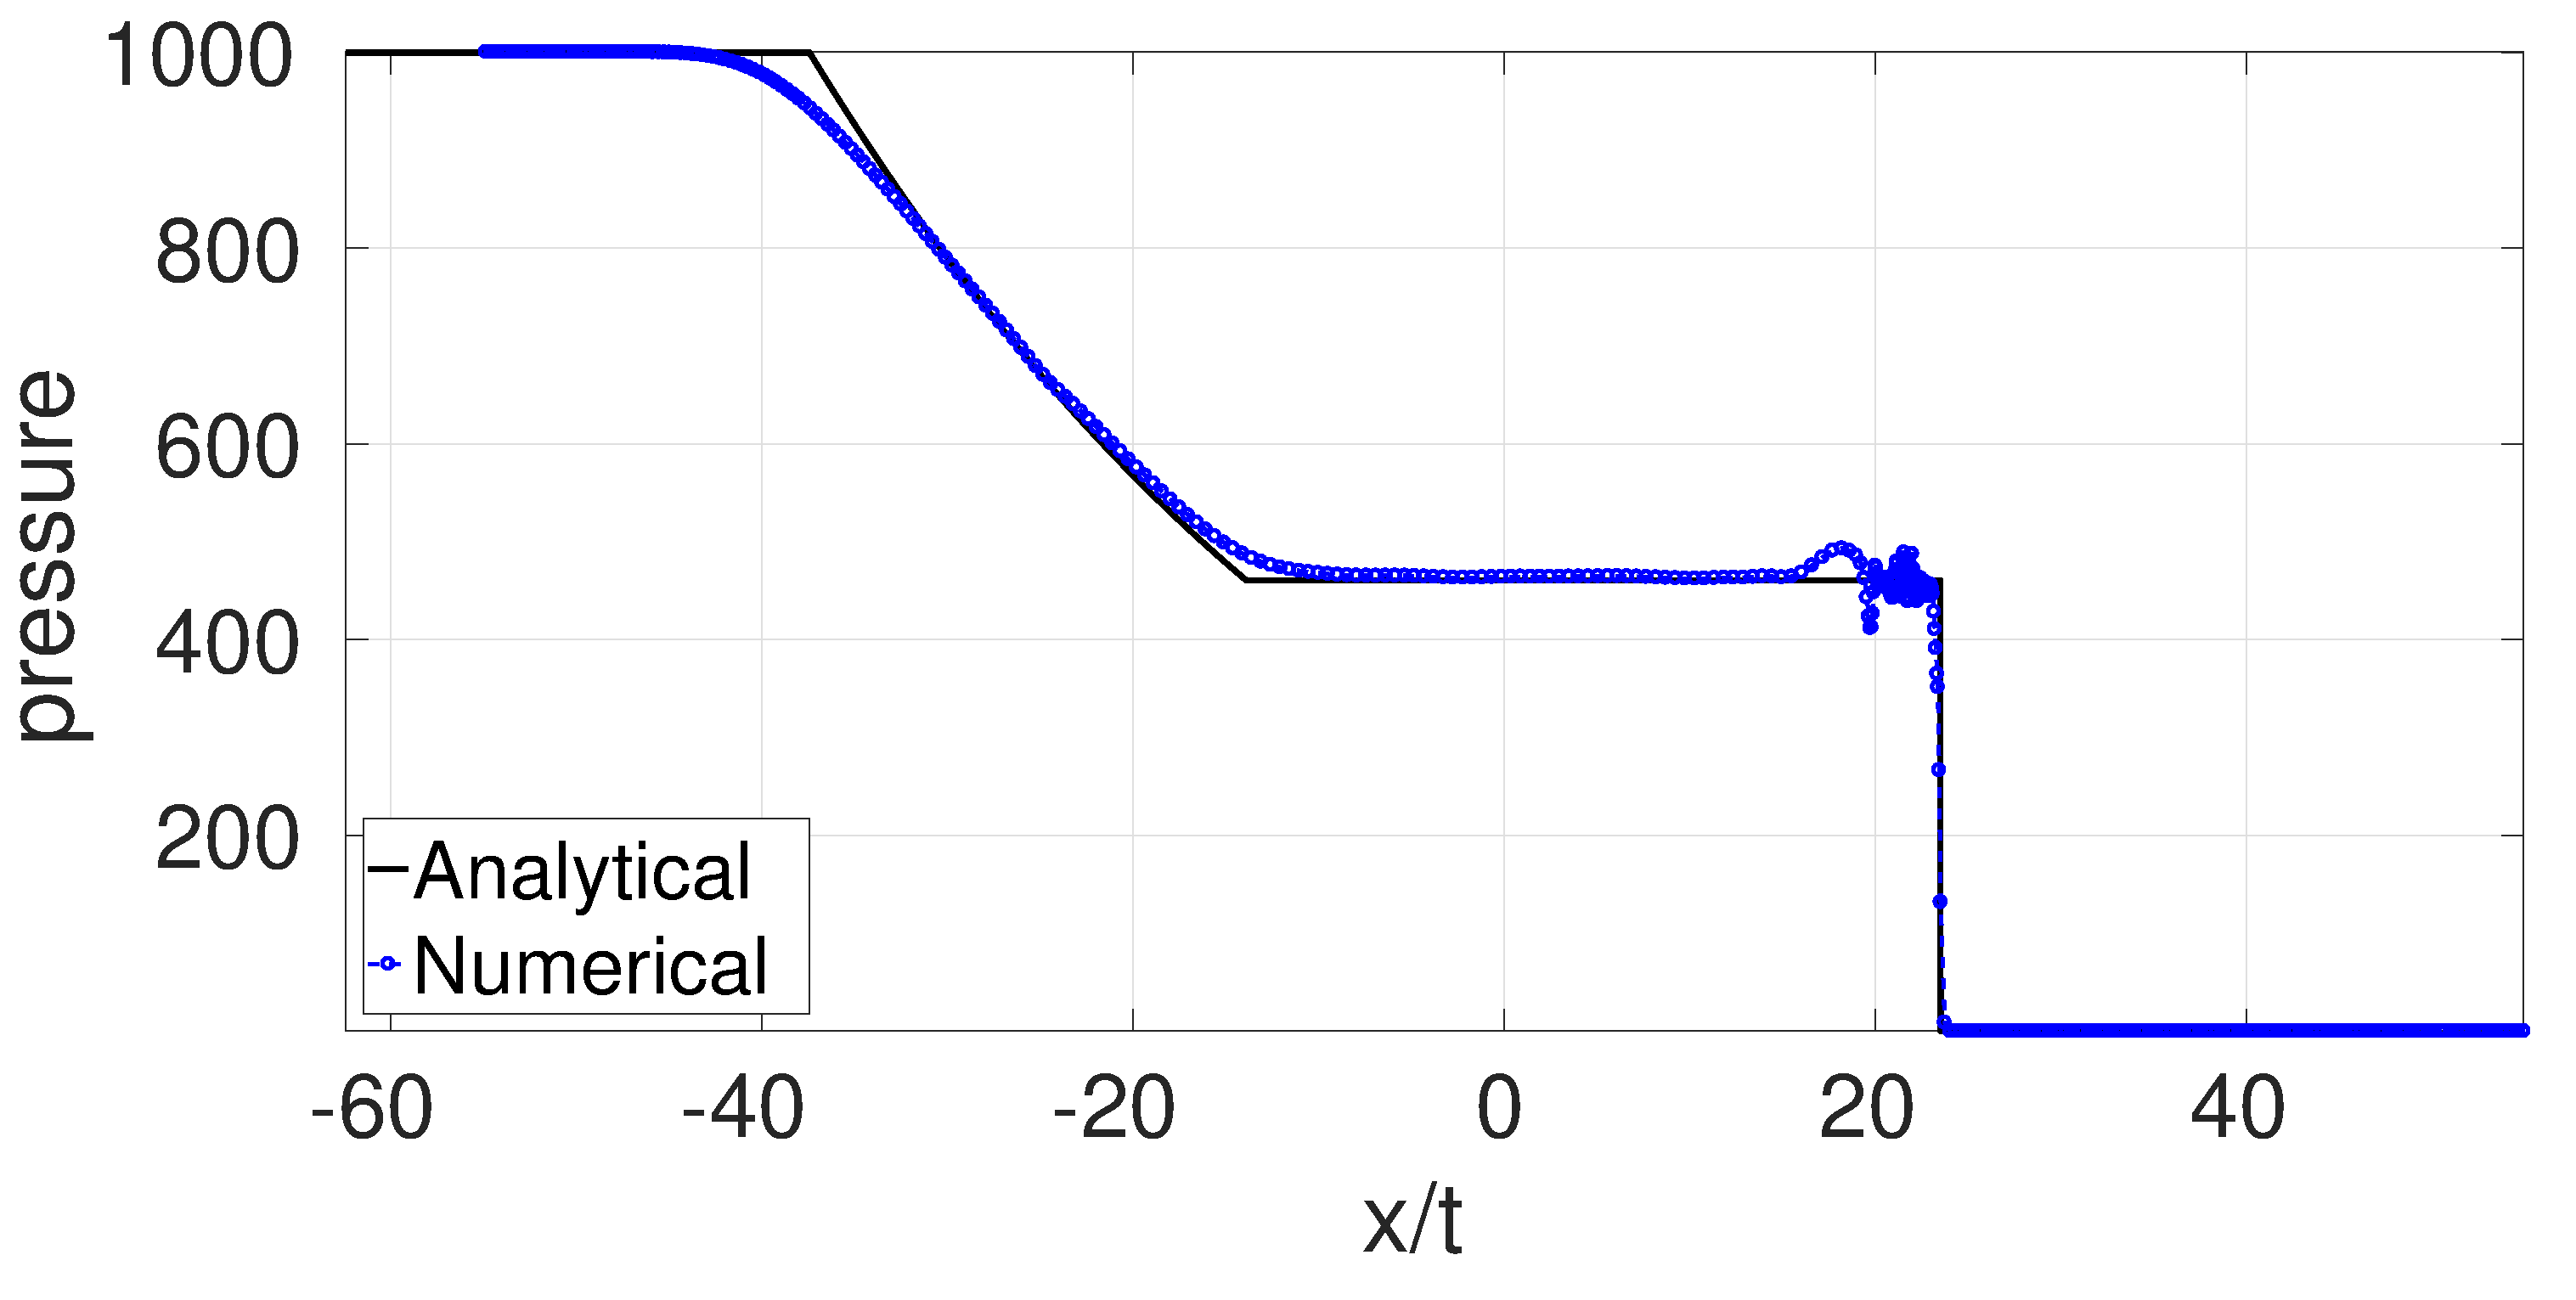
\includegraphics[width=0.99 \textwidth]{Chapter-4/Figures/strong-blast/StrBlst-RCM-p-Rp3}
    \end{minipage}% 
    \caption{Results for test 6, the strong blast test. y axis for density plot is in log base 10. All physical properties are well re-produced. The oscillations between shock and contact discontinuity is relatively larger than other area. A noticeable spike is observed near contact discontinuity.}
    \label{fig:RCM-strong-blast}
\end{figure}

\subsection{3D free jet}
Free jet flow have been studied analytically, experimentally and numerically for many decades, not only because of its wide application but also because of its fundamental significance as a basic flow to the scientific research community. To test the capacity of RSPH for multiple dimensional applications, a free jet flow is simulated in this section by solving 3D compressible Euler Equations using standard SPH, GSPH and RSPH. 
All simulations are using the same setting-up and compared at the same physical time. In this test, RSPH simulation is carried out based on piece wise constant construction of Riemann problem and a HLLC approximate Riemann solver. To do a well-controlled comparison, GSPH adopts the same way for Riemann problem construction and the same Riemann solver as RSPH. 

The computational domain in this test is a box. The boundaries can be categorized into the velocity inlet (a circular area at the center of the bottom of the box), non-slip wall boundary (box bottom) and pressure outlet (other faces of the box). The boundaries are set away from vent to avoid boundary effects on simulation.
At the vent, exit velocity $\textbf{v}$ is set to $500 m / s$ and radius of the nozzle $r$ is set to $8m $. The pressure of ejected fluid are assumed to be the same as ambient ($101 kpa$). The temperature of and ambient fluids are set to $273 K$. 
Velocity is zero for non-slip wall boundary. The heat flux across wall boundary is zero assuming adiabatic wall. The flux of mass should also be zero on the wall. As a result, internal energy flux, which consists of heat flux and energy flux carried by mass flux, vanishes on the wall boundary. 
The pressure of the surrounding ambient is given. As we ignore the viscosity, the shear stress is ignored and normal stress (whose magnitude equals to pressure) balances the ambient pressure.
\begin{equation}
p = p_a\left(z\right)  \label{eq:pressure_bc_p} 
\end{equation} 
Except for the pressure, boundary values for density, velocity, and energy on the outlet are determined by solution. Fluids properties of ideal gas are used in this simulation.

\begin{figure}[H]
    \centering
    \begin{minipage}[t]{.325\textwidth}
        \centering
        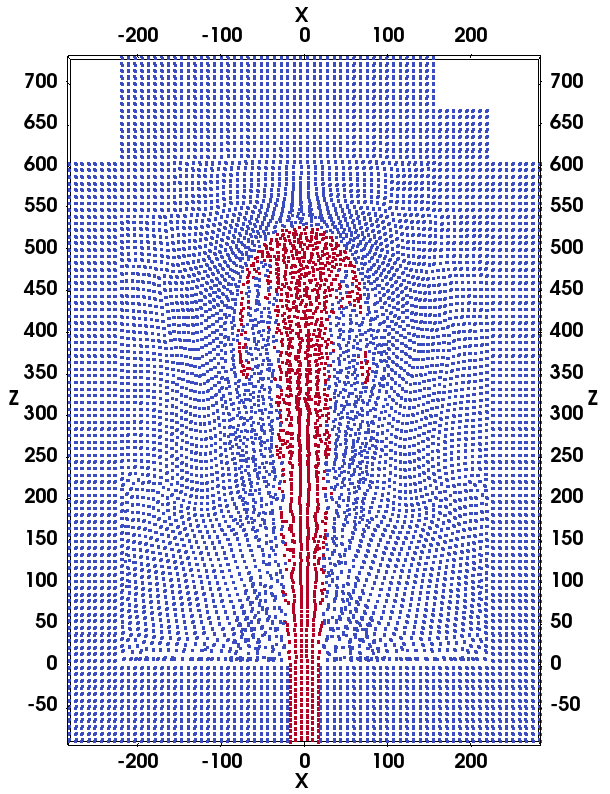
\includegraphics[width=0.99 \textwidth]{Chapter-4/Figures/SPH-alf2-t3-cutView}
    \end{minipage}%
    \begin{minipage}[t]{.325 \textwidth}
        \centering
        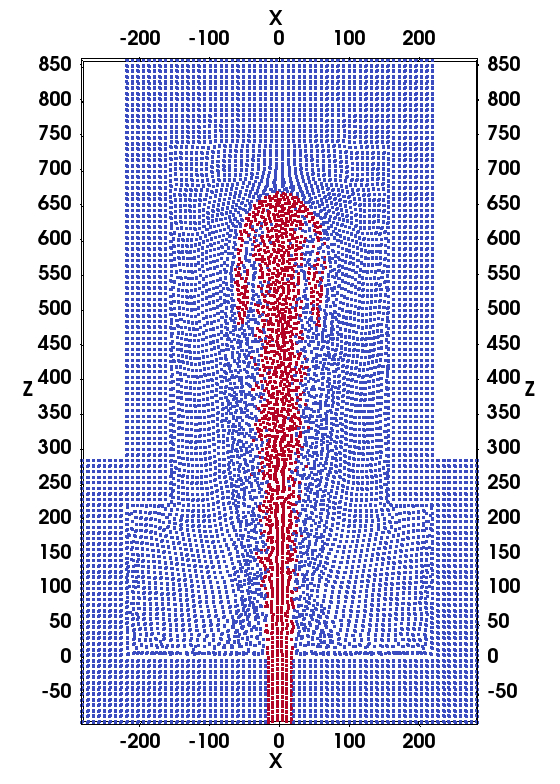
\includegraphics[width=0.99 \textwidth]{Chapter-4/Figures/SPH-alf1-t3-cutView}
    \end{minipage}%
    \begin{minipage}[t]{.325\textwidth}
        \centering
        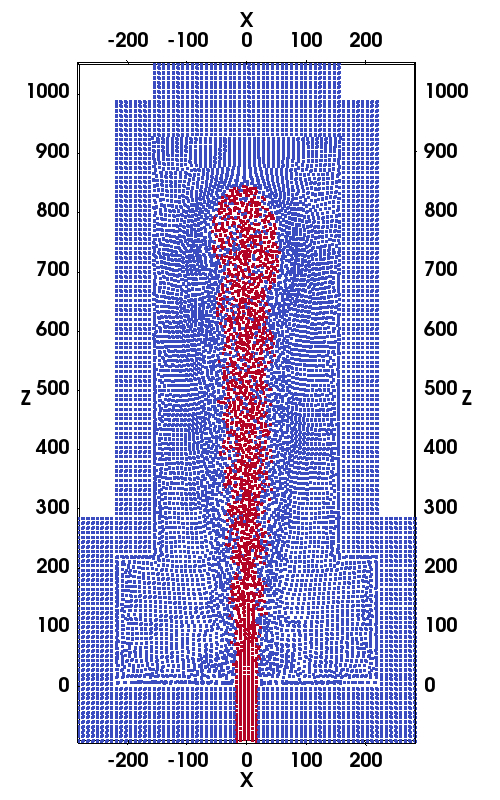
\includegraphics[width=0.99 \textwidth]{Chapter-4/Figures/SPH-alfp3-t3-cutView}
    \end{minipage}%
    \caption{Free jet flow simulation results at $t=3.0 s$ by SPH using different artificial viscosity coefficients. These pictures are front view of a slice of the domain cut by two planes parallel to $x-z$ plane at $y=-9$ and $y=9$. From left to right, the picture is corresponding to $\alpha=0.3$, $\alpha=1.0$ and $\alpha=2.0$ respectively. Another artificial viscosity coefficient $\beta$ is set to be double of $\alpha$ for all tests. Red particles in pictures are particles erupted from the nozzle while blues are ambient fluids particles.}
    \label{fig:free-jet-SPH-comparison}
\end{figure}

\begin{figure}[!ht]
    \centering
    \begin{minipage}[t]{.325\textwidth}
        \centering
        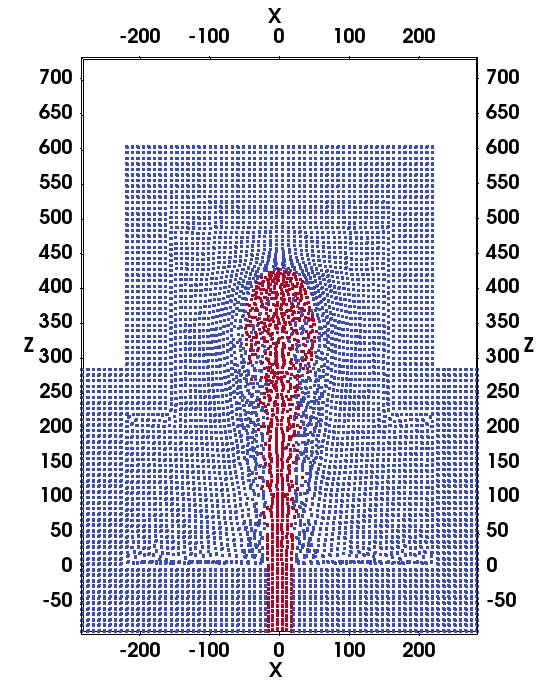
\includegraphics[width=0.99 \textwidth]{Chapter-4/Figures/SPH-alf1-t1p5-cutView}
    \end{minipage}%
    \begin{minipage}[t]{.325 \textwidth}
        \centering
        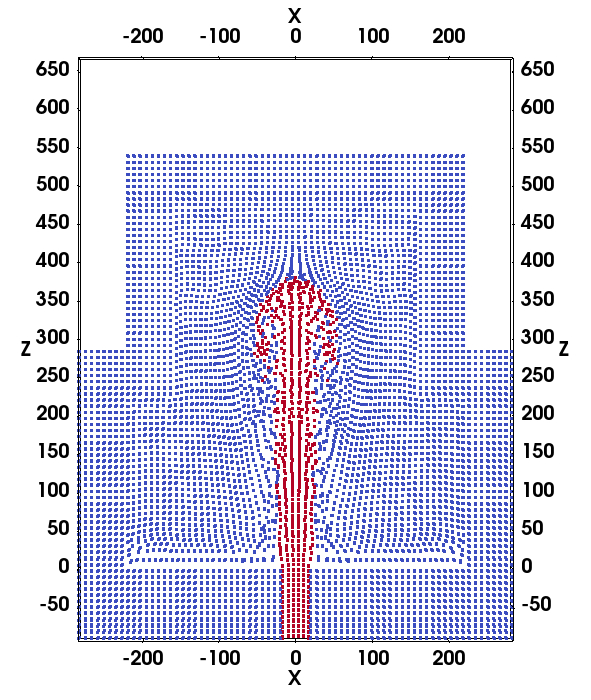
\includegraphics[width=0.99 \textwidth]{Chapter-4/Figures/GSPH-HLLC-t1p5-cutView}
    \end{minipage}%
    \begin{minipage}[t]{.325\textwidth}
        \centering
        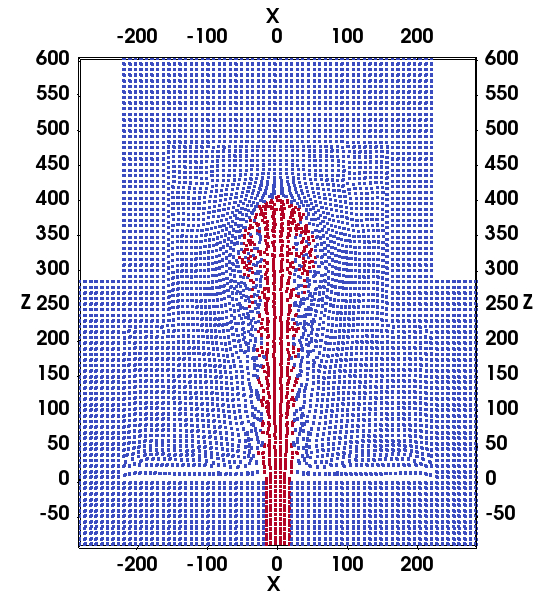
\includegraphics[width=0.99 \textwidth]{Chapter-4/Figures/RSPH-t1p5-cutView}
    \end{minipage}%
    \\
    \centering
    \begin{minipage}[t]{.325\textwidth}
        \centering
        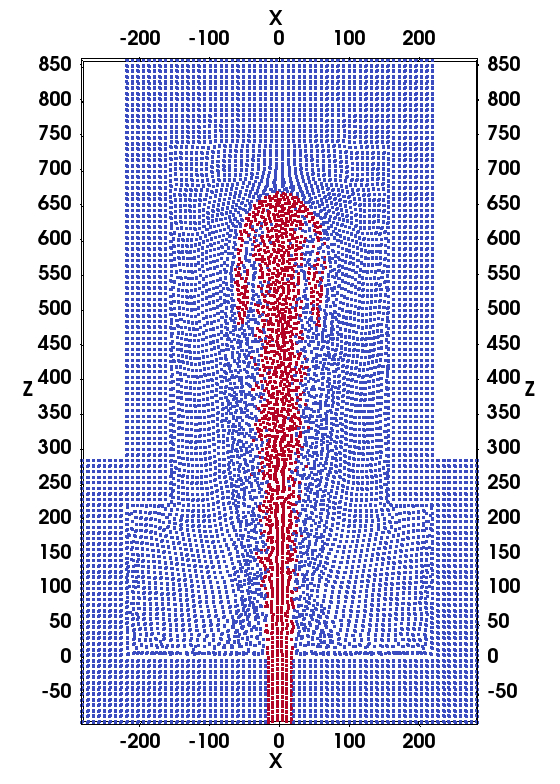
\includegraphics[width=0.99 \textwidth]{Chapter-4/Figures/SPH-alf1-t3-cutView}
    \end{minipage}%
    \begin{minipage}[t]{.325 \textwidth}
        \centering
        \includegraphics[width=0.99 \textwidth]{Chapter-4/Figures/GSPH-HLLC-t3-cutView}
    \end{minipage}%
    \begin{minipage}[t]{.325\textwidth}
        \centering
        \includegraphics[width=0.99 \textwidth]{Chapter-4/Figures/RSPH-t3-cutView}
    \end{minipage}%
    \caption{Simulation results of free jet flow by SPH with $\alpha=1.0, \beta=2.0$, GSPH and RSPH. These pictures are front view of a slice of the domain cut by two planes parallel to $x-z$ plane at $y=-9$ and $y=9$. From left to right, the picture is corresponding to SPH, GSPH and RSPH respectively. Red particles in pictures of the first row are particles erupted from the nozzle while blues are ambient fluids particles. Pictures on the first row are corresponding to $t=1.5s$ while pictures on the second row are for $t=3.0 s$}
    \label{fig:free-jet-comparison}
\end{figure}

Figure \ref{fig:free-jet-SPH-comparison} shows simulation results of the free jet flow by SPH with different artificial viscosity coefficients. The damping effect due to artificial dissipation is clearly shown in this figure. We observe that the lengths to which these jets reach at $t=3.0 s$ are various when using different artificial viscosity coefficient. It is obvious that the larger artificial viscosity, the shorter length the jet can reach. While introducing undesirable damping effects, artificial viscosity is necessary for numerical stability and simulating of shocks. So, in real applications, the artificial viscosity coefficients are usually tuned (see, for example, \citep{gmd-2017-119}) to avoid excessive artificial damping effects.

We compare RSPH with GSPH in terms of equivalent overall artificial damping effects. Different from SPH, both GSPH and RSPH introduce artificial viscosity in an implicit way by solving local Riemann problems. As has been shown in 1D tests, RSPH can introduce less artificial viscosity than GSPH. Fig. \ref{fig:free-jet-comparison} implies that RSPH introduces less overall damping effect than GSPH in 3D application as well, which is consistent with 1D tests. That is to say, RSPH's desirable property of introducing less artificial dissipation in 1D unsteady flow is inherited in 3D applications of RSPH. Recall that RCM shows ability of resolving discontinuities as true discontinuities in 1D unsteady flows but such very desirable property does not persist in genuine two (or higher) space dimensions \citep{colella1982glimm}. Integrating of RCM within the framework of SPH avoids solving higher dimensional Riemann problems overcoming the fundamental shortcoming of RCM.

\section{Conclusion}
We proposed RSPH, a novel SPH scheme for solving hyperbolic non-linear PDEs. The artificial viscosity in RSPH is determined implicitly by randomly sampling solution of a local Riemann problem. No explicit artificial viscosity coefficients is needed. The artificial viscosity introduced by RSPH is demonstrated to be much less than GSPH and SPH without parameter tuning. Besides introducing less amount of dissipation, there are several other attractive features. The pressure ``wiggle" around contact discontinuity, which persists in SPH results, is eliminated in RSPH. It also shows higher order of convergence rate than GSPH when the same construction of local Riemann problem and Riemann solvers. The attractive property of less dissipation persist in multi-dimensional applications.
This new method enables shock capturing with lower dissipation. One potential application of the method is high speed mixing flow, for example, supersonic combustion.
By overcoming a fundamental shortcoming of RCM and inheriting attractive feature of RCM, RSPH provide a powerful numerical method for solving combustion problems in multi-dimensional space.

One shortcoming of RSPH is its inability to completely suppress numerical perturbation caused by non-uniform distribution of smoothing length in space. Such perturbation, as long as it does not lead to numerical instability, is within acceptable range for many tests. However, for very strong shocks, dissipation introduced by RSPH turns out to be not sufficient to stabilize simulation, which finally ends up with negative energy. Since GSPH has been shown introducing more dissipation and hence is more suitable for situation with very strong shocks.

In our investigation presented in this paper, an approximate HLLC Riemann solver is used in place of exact iterative Riemann solver. It would be interesting to see the difference, between using other approximate Riemann solvers and exact Riemann solver. Alternative Riemann solvers, alternative ways for constructing Riemann problems and alternative ways for sampling solution of Riemann problem might also worthwhile for future exploring. In addition, this paper focused on solving of compressible Euler equations. Applications of RSPH in other computational fluids dynamic problems or solving other hyperbolic PDEs are on the list to be explored.
\chapter{Code Architecture and Parallelism}

\section{Introduction}
\label{sect:introduction}
Smoothed particle hydrodynamics (SPH) is a mesh-free scheme, initially developed for astrophysical applications and later extended to computational fluid mechanics. SPH has several features that match well with demands in geophysical flow simulation. It is easier in SPH to include multiple phases and handle complicated geometry and free boundaries. The first implementation of SPH in volcanology was presented by Bursik \cite{bursik2003smoothed} with more developed recently (eg.\cite{ haddad2016smoothed}). The development  of a volcano plume (see Fig. \ref{fig:Plume}) is essentially a multiphase turbulent ejection mixing process accompanied by microphysics phenomena like phase change of water, aggregation, reaction, etc. Accurate prediction of such complicated phenomena in a given time window requires resolution (very high particle counts) that can not be accomplished without parallel computing. Imposing  some types of boundary conditions (such as wind field, eruption boundary condition at the vent) requires dynamically adding and removing particles during simulation. This requires an efficient and flexible data management scheme.\\
Most implementations of the parallel SPH method presented to date are limited to standard SPH and benchmark problems like dam breaks, or relatively
simple scenarios like breaking-waves, flooding, etc. Work on more complicated implementations is relatively rare. Among existing CPU parallel SPH schemes, most of them focus on neighbor searching algorithms and dynamic load balancing. (eg. \cite{ferrari2009new, crespo2015dualsphysics}). Less attention has been paid to developing more flexible data management schemes. 
Fortunately, efficient and flexible data management strategies for parallel computing have been successfully implemented in mesh based methods (eg. \cite{laszloffy2000simple} for adaptive hp finite element method (FEM), and \cite{patra2005parallel} for finite volume method (FVM)). Motivated by these techniques developed for mesh based methods, we present a complete framework for parallelizing SPH program with the MPI standard allowing flexible and efficient data access.\\
Any implementation of SPH requires efficient searching and updating of neighbors during the simulation. Of the many possible choices we adopt the popular background grid method \cite{monaghan1985refined}, which is also used for domain decomposition. We refer to the elements of the background grid as buckets. 
As for the actual storage of data representing the physical quantities associated to each particle, different strategies have been adopted in existing implementations of SPH. 
In DualSPHysics\cite{crespo2015dualsphysics}, the physical quantities of each particle (position, velocity, density...) are stored in arrays, and the particles (and the arrays with particle data) are reordered following the order of the cells. It is not flexible enough to add, delete and especially access particles for such fixed-size arrays. Ferrari\cite{ferrari2009new} adopted linked lists using pointers so that particles can be deleted or added during the simulation. Storage problems caused by fixed-size arrays are thereby also eliminated. We adopt hash tables to store pointers to objects of particles and buckets, which give us not only flexibility of deleting and adding of elements, but also quicker access compared with linked lists. A SFC-based index is adopted to give each particle and background bucket an unique identifier -- a strategy known to preserve some locality at minimal cost. The SFC based numbering strategy is further extended to include time step information so that particles added at the same position but different time will have different identifiers. 
We adopt an easy-programming scheme based on SFC \cite{patra1999efficient} to decompose the domain.\\
To the best of the author's knowledge, no current implementation of SPH has the feature of adjusting the computational domain based on simulation needs. For volcano plume simulation, this feature will greatly reduce computational cost by avoiding computing of uninfluenced fluids. This feature is accomplished by adding a scan function to monitor the outermost layer of the domain and turn ghost particles to real particles at the proper time thus effectively defining a halo domain with an almost optimally defined size.\\
\section{Data Structure and Load Balance}
\begin{figure*}[!t]
\centering
\includegraphics[scale=0.32]{Chapter-5/Figures/Work_flow}
\hfil
\includegraphics[scale=0.32]{Chapter-5/Figures/Work_flow_adjust}
\caption{Workflow for SPH code. Figure to the left is the basic workflow. The right figure is the workflow that enables dynamic halo domain.}
\label{fig:Work_flow}
\end{figure*}
In SPH, the domain is discretized by particles and the position of each particle is updated at every time step. The physical laws written in the form of partial differential equations need to be transformed into the Lagrangian particle formalism of SPH. Using a kernel function that provides the weighted estimation of the physical properties in the neighborhood of a discrete point (particle), the integral equations are evaluated as sums over neighbor particles. Only particles located within the support of the kernel function will interact. Thus, physical properties associated with the particle are updated based on its neighbors. A neighbor search therefore needs to be carried out before updating physical properties. A basic workflow of our SPH code is shown in Fig. \ref{fig:Work_flow}. We use buckets, which contain all particles associated with a sub-domain (see Fig. \ref{fig:SFC_domain_decomposition}) 
and keep them stationary during the entire simulation, to reduce searching cost (since the search can now be restricted to only neighboring domains).
Domain is decomposed based on a SFC going through centroids of all buckets, as shown in Fig. \ref{fig:SFC_domain_decomposition}.
\subsection{SFC based indexing}
Our data structure starts from assigning each particle and bucket an identifier, we refer to it as a key, which should be unique throughout the simulation. The key for a bucket is determined by the centroid coordinate of the bucket while the key for a particle is determined by adding coordinates and time step of the particle. The map from coordinates to key is based on SFC \cite{sagan2012space} which maps a n-dimensional domain to a one dimensional sequence. The standard procedure for obtaining the SFC is: 
\begin{itemize}
\item Scale all coordinates in computational domain ($\textbf{X}^\prime$) into an $n$ dimensional unit hypercube $[0,1]^n $: $\textbf{X}^\prime \rightarrow \textbf{X}$, where $\textbf{X}$ represents coordinates in the hypercube.
\item Compute $k_r = h_n(\textbf{X})$. Where $h_n$ is the map $h_n: [0,1]^n \rightarrow [0,1]$. 
\item Convert $k_r$ to integer $k$ by multiplying $k_r$ with a large integer and removing decimal part.
\item Sort all keys to form a SFC sequence. The SFC represents a curve passing through all particles (or centroids of buckets).
\end{itemize}
%
\begin{figure*}[!t]
\centering
\includegraphics[scale=0.17]{Chapter-5/Figures/SFC_particles_buckets}
\hfil
\includegraphics[scale = 0.18]{Chapter-5/Figures/SFC_particles_buckets_partition}
\caption{The left figure shows SFCs passing all particles and buckets. The right figure shows an example of a domain decomposition based on the SFC of buckets.}
\label{fig:SFC_domain_decomposition}
\end{figure*}
%
Details for constructing the map $h_n$ can be found in \cite{patra1995problem}. These keys denote a simple addressing and ordering scheme for the data, i.e., a global index space for all the objects.\\
In some situations, new particles need to be added during the simulation. For example, new particles need to be added at the bottom of the eject vent (see Fig. \ref{fig:Particle_adding_with_link}). To assign distinct identifiers for particles added at the "same position" but at different time steps, we extend the SFC-based key to a time-dependent SFC based key by including date of birth of particles into their keys. The time-dependent SFC based key can be denoted as: $[k,t]$, where $t$ is the time step. The map $h_n$ will become:
\begin{equation}
h_n: [0,1]^n \times \textbf{T} \rightarrow [0,1] \times \textbf{N}
\end{equation}
Where $\textbf{T} \subset [0,\infty)$ is the time dimension, and $\textbf{N}=\lbrace 0, 1, 2, 3...\rbrace$.
To guarantee locality, sorting of particle keys is based on $k$, that is to say, particles with smaller $k$ always come before particles with larger $k$. For particles that have the same $k$, ordering will then depend on $t$. Figure \ref{fig:SFC_domain_decomposition} shows SFC ordering of buckets and particles in buckets. 
Several features of this indexing scheme are suitable for SPH:
\begin{itemize}
\item Guaranteed uniqueness of keys.
\item The key of each object is generated purely based on its own coordinates. When we add new objects on different processes, the key of each object can be generated fast and independently.
\item Objects that are located closely in the Euclidian space will also be close to each other in the one dimensional SFC key space in a mean sense. Since SPH particles only interact with their neighbors, geometric locality can be exploited for efficient access of data.
\item This type of key effectively generates a global address space. Globalism of key and conservation of spatial locality make it easy to partition the sorted key sequence and obtain a decomposition of the problem.
\end{itemize}
\subsection{Data management strategies}
%\subsubsection{Particle and bucket}
The most basic data structure of SPH are particles and buckets. Both are defined as C++ classes. Information that is contained in particle objects can be categorized into six categories: identifier (the key), affiliate(rank of the process that the particle belongs to), primitive variables (variables in governing equations, e.g. density, velocity), secondary variables (physical properties that can be computed from primitive variables, they are stored to avoid repeated computations, e.g., pressure and temperature), flags (indicators, such as indicator for ghost particle or real particle) and neighbor information (it is a vector of particle keys in our application). Similarly,  information that is contained in a bucket object can also be categorized into different categories: identifier, affiliate, dimension information (maximum and minimum coordinates, boundary information), flags (indicators, such as guest indicator, which is used  to indicate whether the bucket belongs to another adjacent subdomain or not), neighbor information (keys of 27 neighbor buckets including its own key) and owned particles (it is a vector of particle keys in our application). Objects are then accessed through hash tables.\\
%\subsubsection{Hash table and hash collision}
One of the fundamental data structures that allows flexible data access is a hash table. Based on the keys of data, the address-calculator(hashing) function determines in which slot the data should be stored:
\begin{equation}
Index = hash(key)
\end{equation}
Data in a hash table can be accessed with time complexity of O(1) when there is no hash collision. One way to handle hash collisions is to use an additional sorted vector attached to the hash table. When several keys hash to the same index, a vector will be created. The vector is sorted based on keys so that a binary search (with an average time complexity of O(log n)) can be used to find the correct position for adding, deleting or retrieving of data. Another option is using an additional linked list which is more flexible in memory allocation but slower in searching (O(n)). In addition, pointer based memory accessing of linked lists will greatly slow down the efficiency of data access for long linked lists. Choosing the proper way to handle hash conflicts greatly depends on the problem itself. For volcano plume simulation, new particles are added at the bottom of the eruption vent (see Fig. \ref{fig:Particle_adding_with_link}), making the linked list a better choice. Pointers to these new particles will be stored in external linked lists as shown in Fig. \ref{fig:Particle_adding_with_link}.
\begin{figure}
\centering
{\includegraphics[scale=0.28]{Chapter-5/Figures/Particle_adding_with_link}}
{\caption{Non-uniform distribution of particles in the $[0,1]^n \times \textbf{T}$ space due to adding of new particles at a small area of the whole domain.}
\label{fig:Particle_adding_with_link}}
%\killfloatstyle
%\ffigbox
{\includegraphics[scale=0.34]{Chapter-5/Figures/int_bar}}
{\caption{The influence of different load balance check intervals on simulation time. The bar values are the extra simulation time in log scale. The optimized interval is 3s.}
\label{fig:check_int}}
%\end{floatrow}
\end{figure}
%\subsubsection{Hash function for time dependent key}
For time-independent keys, the hash function can be a simple function like:
\begin{equation}
Index= \frac{Key - Min\,Key}{Max\,Key - Min\,Key} 
\times Hash\,Table\,Size 
\label{eq:hash_function}
\end{equation}
One natural way to hash time-dependent keys $[k,t]$ is to convert the two elements in the key into one number taking $k$ as the higher digit and $t$ as the lower digit of the large number. However, for volcano plume simulation, only ghost particles for eruption boundary condition will be successively added at the same place: the bottom of the vent. That is to say, particles are distributed non-uniformly in the $[0,1]^n \times \textbf{T}$ space as shown in Fig. \ref{fig:Particle_adding_with_link}. To avoid a non-uniform sparse hash table and conserve spatial locality, we only plug the first number, $k$, of the key, $[k,t]$, into the hashing function, Eq. (\ref{eq:hash_function}). All particles with the same birth location will hash to the same index and be handled by external linked lists.
\subsection{Domain decomposition and load balancing strategy}
\label{sect:load_balance}
%\subsubsection{Weighted work load} \label{sec:Weighted_work_load}
Particles in our problem can be categorized into four types: real particles, wall ghost particles, pressure ghost particles and eruption ghost particles. Ghost particles are for imposition of corresponding boundary conditions (See Fig. \ref{fig:Plume}). As different types of particles involve different amount of computational work, shown by table \ref{tab:Computational_cost_steps}, we assign different work load weights for different types of particles based on profiling data. Instead of simply using number of contained particles as work load for buckets, work load of each bucket is determined by summing up work load weights of all particles within the bucket. The SFC of buckets now becomes a weighted sequence. Domain decomposition  is conducted by cutting the weighted SFC of buckets into pieces. Each piece of the SFC should then have a balanced total work load.
\begin{figure}
\centering
%\CenterFloatBoxes
%\ttabbox
%{	  
	  \begin{tabular}{lrrrrrr}
	    \hline
	    Step & Cost ($ms$) & Real & wall & eruption & pressure\\
	    \hline
	    neighbor search & 0.41 & Yes & No & No & No \\
	    update momentum and energy & 0.70 & Yes & No & No & No\\
	    update density & 0.42 & Yes & No & No & No \\
	    update position & 0.01 & Yes & No & Yes &  No\\
	    velocity filtering& 0.43 & Yes & No & No & No\\
	    apply wall boundary condition     & 0.75 & No & Yes & No & No\\
	    summation ($ms$) & - & 1.97 & 0.75 & 0.01 & 0.00\\
	    \hline
	  \end{tabular}
%}
{\caption{Computational cost per particle for different steps}	}
\label{tab:Computational_cost_steps}
\end{figure}

%\subsubsection{Domain decomposition and dynamic load balancing}
Figure \ref{fig:SFC_domain_decomposition} shows how the domain is decomposed based on partition of the SFC of buckets. The particles are automatically split into several groups along with buckets that contain them. As the SFC of buckets is a curve in three dimensional (3D) space, partition of this curve will automatically lead to 3D domain decomposition. 
Movement of particles, addition of new particles, and adjustments of domain will lead to significant load imbalance between processes. To restore load balance, computational load is monitored at a given interval which is optimized based on numerical experiments. Repartitioning is carried out when load imbalance is larger than a given tolerance.
\\
As some of the neighbor particles reside in other partitions, a set of ``guest'' particles and buckets are used to synchronize data across partitions. To minimize communications, data is synchronized only where needed, using non-blocking MPI communications. 
\section{Dynamic Halo Domain} 
For plume simulation and similar phenomena, where some fluid ejects into a stationary fluid and gets mixed, the stationary fluid must be represented.
A lot of CPU time will be spent on computing associated with these stationary particles. If simulation of stationary particles can be avoided, the computational cost will be greatly reduced.
We propose a simple strategy to add such a feature to our code with low computational cost. We add a scan function to monitor the outermost layer of the domain. When the ejected fluid reaches the boundary of the current domain, pressure ghost particles (light blue particles in the right figure of Fig. \ref{fig:Plume}) will be turned to real particles (red particles in the right figure of Fig. \ref{fig:Plume}) and then add a new layer of pressure ghost particles for pressure boundary conditions. Wall ghost particles (grey particles in the right figure of Fig. \ref{fig:Plume}) will also be added when necessary. The original workflow is modified to enable such a feature. The modified workflow is shown on the right in Fig. \ref{fig:Work_flow}).\\
An involvement flag is added to particle class to distinguish different states of involvement. Particles are categorized into three groups based on the value of the involvement flag: involved, potentially involved, and not involved. The involved particles are particles that have already been affected by the mixing. The potentially involved particles are particles that have not been involved in mixing but are adjacent to involved particles and will thus be involved in the near future. 
All communication and computation associated with uninvolved particles can be ignored. That is to say, only potential involved and involved particles need to be simulated.
As simulation progresses, the ejected fluid will reach a larger area and more and more particles will be influenced. When originally stationary air is influenced by erupted material, the mass fraction of the erupted material will increase from zero to a positive value. So we can determine whether a particle should turn to involved status based on whether the mass fraction of that particle is larger than a given threshold ($10^{-5} $ in our simulation) or not. Other physical properties, like velocity, can also serve as alternative ``switch criteria.''\\
A similar scheme is also deployed for buckets resulting in a categorization of buckets. The additional complexity is that potentially involved ghost particles must also be taken into accounted.
\begin{figure*}[!t]
\centering
\includegraphics[width=3.4cm,height=3.8cm]{Chapter-5/Figures/plume_photo}
\hfil
\includegraphics[width=5.0cm,height=3.8cm]{Chapter-5/Figures/Plume_simulation}
\hfil
\includegraphics[width=4.8cm,height=3.8cm]{Chapter-5/Figures/Boundary-condition}
\caption{The left figure shows a plume photo of Sakurajima Volcano eruption, the middle figure shows a typical simulation results with the same input parameters as "Run P1" in reference \cite{suzuki2005numerical}. The right figure is a cross-section view of the computational domain, it illustrates how particles are deployed on different boundaries: red are real particles, dark blue are eruption ghost particles, grey are wall ghost particles, the light blue are pressure ghost particles.}
\label{fig:Plume}
\end{figure*}
\section{Numerical Test}
We use the same governing equations and input parameters as the plume simulation presented by Suzuki \cite{suzuki2005numerical}. %Details about discretization of the governing equations will not be covered in this paper, neither. 
A typical simulation result of volcano plume by our code is shown in Fig. \ref{fig:Plume}.
%
\subsection{Scalability test}
\begin{figure*}[!t]
\centering
\includegraphics[scale=0.31]{Chapter-5/Figures/strong_scale}
\hfil
\includegraphics[scale=0.31]{Chapter-5/Figures/strong_scale_zoom}
\hfil
\includegraphics[scale=0.31]{Chapter-5/Figures/weak_scale}
\caption{The left figure shows strong scalability tests result. middle figure is the zoomed view of first one. It is obviously shown that strong scalability is better when the problem size is larger. The right figure is weak scalability test results}
\label{fig:2cases_efficiency}
\end{figure*}
%
Experiments have been carried out on the computational cluster of Center for Computational Research (CCR) at Buffalo. 
The compute servers have 12 cores (two Xeon E5645 processors per server) running at 2.40GHz clock rate with 4GB memory per core on a Q-Logic Infiniband network. Main memory and level 3 cache are shared on each node. The simulation domain is a box with initial dimension $[-4.8km, 4.8km]\times [-4.8km, 4.8km] \times [0km, 6km]$ for case 1 and $[-10km, 10km]\times [-10km, 10km] \times [0km, 5km]$ for case 2. The smoothing length (we set initial intervals between particles equal to smoothing length) equals to 200m and 100m respectively for test case 1 and test case 2. So the computational work load of test case 2 is larger than that of the test case 1. The simulations run for 20s physical time.  Parallel speed up is shown in Fig. \ref{fig:2cases_efficiency}. Test case 2 shows better speed up than test case 1 which implies that strong scalability can be improved by increasing total amount of work load.
The weak scalability test is conducted with the same initial domain as test case 1 and various smoothing length. Each simulation runs for 400 time steps. The average number of real particles for each process keeps constant at $25900$, so the average work load for each processor is approximately constant. 
Right side figure in Fig \ref{fig:2cases_efficiency} shows the timing of a weak scalability test.\\
\subsection{Effect of workload check interval and calibrated particle weight}
\begin{figure}
\centering
%\CenterFloatBoxes
%\ttabbox
{	  
	  \begin{tabular}{lrrrr}
	    \hline
	    Physical time & 10 s & 20s & 30 s & 40 s \\
	    \hline
	    Same weight & 1141.7 & 4119.4 & 10371.0 & 12453.7\\
	    Different weights & 1108.2 & 4057.0 & 10281.5 & 12166.3\\
	    \hline
	  \end{tabular}
}
{\caption{Simulation time for the same particle weight and different particle weights at different physical times.}}
\label{tab:same_diff_particle_weight}
\end{figure}
In section \ref{sect:load_balance}, we proposed to use different particle weights for different types of particles when estimate the workload of buckets. The effect of using different particle weight is demonstrated in table \ref{tab:same_diff_particle_weight}. The simulation time is reduced by using different particle weights. However, the amount of time that is reduced is not as significant as we expected. One possible explanation is that real particles are the major population, so the load imbalance caused by assigning improper weight values to ghost particles is small.\\
The best load balance check interval is calibrated based on a series of simulations with different load balance scan intervals. From 0 - 50 seconds physical time, the interval of 1 second shows a better load balance than interval of 2 seconds. However, for the simulation of 50 - 100 seconds, interval of 2 seconds is better. This implies that loss of load balance accumulates faster and requires a more frequent re-decomposition of domain at the early stages of simulation. This is consistent with the plume development process: the domain grows quickly at the beginning as erupted material ejects into the environment and spreads. Afterwards, the spreading speed of the front edge slows down due to viscosity and momentum exchange leading to slowing down of domain growth. We need to emphasize that, these optimized parameters, including weights of particles and load balance checking interval, are case sensitive and need to be re-calibrated for different applications and hardware architecture.
%
\subsection{Effect of dynamic halo domains}
\begin{figure}
\centering
%\CenterFloatBoxes
%\begin{floatrow}
%\ttabbox
{	  
    \begin{tabular}{lrr}
    \hline
    Functions & Total time (s) & Called times\\
    	\hline
    UPME & 2954.8 & 201 \\
    UPP & 38.55 &  201 \\
    ADPP & 21.51 & 3 \\
    ADWP  & 8.88 & 3 \\
    SWCH & 0.08 &  2 \\
    SCN  & 7.72 & 201 \\
    \hline
  \end{tabular}
}
{\caption{Computational work load of extra steps for domain adjusting. SWCH represents step that switch pressure ghost particle to real particle, ADPP is short for adding new pressure ghost particles, ADWP represents adding wall ghost particles, SCN is short for scanning the outmost layer of the domain.  Momentum and energy update (UPME) and position update (UPP) also included for comparison.}
\label{tab:Computational_cost_doamin_adj}}
\centering
{\includegraphics[scale=0.35]{Chapter-5/Figures/adj_vs_no}}
{\caption{The figure on the top shows execution time without domain adjusting, the figure on the bottom shows execution time with domain adjusting. Different bins represent execution time up to specific physical time indicated by horizontal axis.}
\label{fig:adj_vs_no}}
%\end{floatrow}
\end{figure}
For the test problem in this paper, the volcano plume finally reaches to a region of $[-10km \,\,\, 10km] \times [-10km\,\,\,10km] \times [0km\,\,\,20km]$ after around 300 seconds of eruption. When numerical simulation goes up to 90 seconds, the plume is still within a region of $[-3km\,\,\,3km] \times [-3km\,\,\,3km] \times [0km\,\,\,6km]$. This implies that adjusting of domain can avoid computing large number of uninfluenced particles, especially for the early stages of simulation. On the other hand, additional functions (see Fig. \ref{fig:Work_flow}) for domain adjusting will add extra computational cost. Table \ref{tab:Computational_cost_doamin_adj} shows the extra computational cost corresponding to these functions. Profiling data for momentum and energy update (UPME) and position update (UPP) is also included in the table for the purpose of comparison. As we can see from the table, the cost of SCN is even smaller than UPP function, which is the cheapest function (as shown in table \ref{tab:Computational_cost_steps}) in the regular workflow (see Fig. \ref{fig:Work_flow}). The other three functions, ADPP, ADWP and SWCH, are only called a few times during the simulation, and as a consequence, the extra computational cost due to them are negligible. To summarize, the additional cost caused by the domain adjusting functions is ignorable.
Figure \ref{fig:adj_vs_no} shows that simulation time of the test problem is greatly reduced when we adopt the domain adjusting strategy in our code.
\section{Conclusion}
We developed data management strategies for a MPI-parallel implementation of the SPH method to simulate volcano plumes. Neighbor searching and domain decomposition is based on the background grid. A SFC based index scheme is adopted to identify buckets and time-dependent SFC keys are used as identifiers for particles. 
Hash tables with external linked lists are adopted for accessing particles and buckets data. Based on calibrated particle weights, a dynamic load balance strategy is developed by checking load balance and re-decomposing the domain at an optimized interval. The performance of the code was further improved by several factors by adjusting the computational domain during simulation.
Overall we obtain good scalability and performance.\\
The flexibility of our data access methodology enables implementing mesh-free methods for solving more complicated problems and using more advanced techniques, such as dynamic particle splitting techniques\cite{vacondio2012accurate, feldman2007dynamic}, which will give higher resolution at the area of interest by splitting one large particle to several smaller ones. The data structure, particle and bucket indexing strategies, domain decomposition, dynamic load balancing method and domain adjusting strategies in this paper can be adopted to other mesh-free methods (not just SPH).

\chapter{Verification and Case Studies}

\section{Introduction}
SPH is a mesh-free Lagragian method. In SPH, the domain is discretized by a set of particles or discretization points and the position of each particle is updated at every time step based on the motion computed. Approximation of all field variables (velocity, density and pressure, ect.) is obtained by interpolation based on discretization points. The physical laws (such as conservation laws of mass, momentum and energy) written in the form of PDEs (partial differential equations)  or ODEs (ordinary differential equations) need to be transformed into the Lagrangian particle formalism of SPH. Using a kernel function that provides the weighted estimation of the field variables at any point, the integral equations are estimated as sums over particles in a compact subdomain defined by the support of the kernel function associated with the discretization points. Thus, field variables associated to the particle are updated based on its neighbors. Each kernel function has a compact support determined by smoothing length of each particle. There are several review papers by \citet{monaghan1992smoothed, monaghan2005smoothed, rosswog2009astrophysical, price2012smoothed, monaghan2012smoothed}, giving a pretty comprehensive view over SPH. We only refer here to the representation of the constitutive equations in SPH and put more focus on specific numerical techniques for plume modeling.

We present a series of numerical simulations to verify and validate our model in this section. Plume-SPH is first verified by 1D shock tube tests then by a JPUE (jet or plume that is ejected from a nozzle into a uniform environment) simulation. Velocity and mass fraction distribution both along the central axis and cross transverse are compared with experimental results. The pattern of ambient particles entrainment is also clearly shown. Then a simulation of representative strong volcanic plume is conducted. Integrated local variable are comparable with simulation results from existing 3D plume models.

\section{1D Shock Tube Tests}
1D shock tube tests are first conducted to verify our code. Input parameter of each tests can be found in Table \ref{tab:1D-shock-input_parameters}. These tests can represent typical cases in 1D.
Test 1 consists of a left rarefaction, a right travelling contact and a right shock. Density decreases at down wind of contact wave.
Test 2 also consists of a left rarefaction, a right travelling contact and a right shock. Density increases at down wind of contact wave.
Test 3 is a double expansion test with different initial dnesity.

\begin{table}[htp]
\centering
      \caption{Input parameters of 1D shock tube tests}		
	  \begin{tabular}{lrrrrrrr}
	    \hline
	          & $\rho_L$ & $p_L$ &$v_L$ & $\rho_R$ & $p_R$ &$v_R$ & $t_f$\\
	    \hline
	    Test 1 & $1.0$ & $1.0$ &$0$ & $0.5$ & $0.2$ &$0$ & $0.2$\\
	    Test 2 & $1.0$ & $1.0$ &$0$ & $0.25$ & $0.1795$ &$0$ & $0.17$\\
	    	Test 3 & $2.0$ & $1.95$ &$1.0$ & $1.0$ & $1.95$ &$-1.0$ & $0.13$\\
	    \hline
	  \end{tabular}
	  \label{tab:1D-shock-input_parameters}
\end{table}

In  table \ref{tab:1D-shock-input_parameters},  subscript $L$ refers left side and $R$ for right side, $t_f$ is the total simulation time. The initial interval between two adjcent particles is 0.03. The computational domain is $[-0.4, 0.4]$. The specific internal energy is is compared against exact solutions. As shown in Fig. \ref{fig:1D-shock-tests-verification}, the position and magnitude of the waves are correctly predicted. The fluctuations near the contact discontinuity are caused by sharp change of smoothing length.

\begin{figure}[!htb]
    \centering
    \begin{minipage}{.325\textwidth}
        \centering
        \includegraphics[width=0.99 \textwidth]{Chapter-6/Figures/GSPH-Sod-verification-e}
    \end{minipage}%
    \begin{minipage}{.325 \textwidth}
        \centering
        \includegraphics[width=0.99 \textwidth]{Chapter-6/Figures/Sod-verification-e}
    \end{minipage}%
    \begin{minipage}{.325 \textwidth}
        \centering
        \includegraphics[width=0.99 \textwidth]{Chapter-6/Figures/d-exp-verification-e}
    \end{minipage}%   
    \caption{Comparison of specific internal energy of simulation results agaist analytical results for shock tube tests. The plots from left to right are corresponding to test 1, test 2 and test 3 respectively.}
    \label{fig:1D-shock-tests-verification}
\end{figure}

\section{Simulation of JPUE}
JPUE can be considered as a simplified volcanic plume. While the effect of stratified atmosphere and the effect of expansion due to high temperature in volcanic plume are not represented, JPUE reproduces the entrainment due to turbulent mixing which is one of the key elements in volcanic plume development. There exist consistently good experimental data \citep { list1982turbulent,dimotakis1983structure, papanicolaou1988investigations, ezzamel2015dynamical} that describe the JPUE flow field giving an insight into details of JPUE, such as transverse velocity and concentration profile. In this section, we verify that our code and the $SPH-\varepsilon$ turbulence model is able to reproduce feature of turbulent entrainment by a JPUE simulation.

As many of these experiments were conducted with liquid, we replace the original equation of state (Eq. (\ref{eq:EOS})) with a weakly compressible Tait equation of state \citep {becker2007weakly} (see Eq. (\ref{eq:EOS-Tait})) to avoid solving the Poisson equation.
\begin{equation}
p=B\left[\left(\dfrac{\rho}{\rho_0}\right)^{\gamma}-1\right]
\label{eq:EOS-Tait}
\end{equation}
with $\gamma=7$ and $B$ is evaluated by:
\begin{equation}
B=\dfrac{\rho_0 c^2}{\gamma}
\end{equation}
where $c$ is the speed of sound in the liquid. The energy equation is actually decoupled from the momentum conservation equation and the mass conservation equation by using this equation of state (EOS). In addition, the "atmosphere" is assumed to be uniform and gravity is set to be zero. We set the temperature and density of ejected material the same as surrounding ambient. This further simplifies the scenario for the convenience of studying turbulent mixing. 

One overall feature of JPUE is "self-similarity" which means that the evolution of the JPUE is determined solely by the local scale of length and velocity which theoretically account for the fact that the rate of entrainment at the edge of JPUE is proportional to a characteristic velocity at each height. As a results, physical and numerical experiments do not necessary to have exactly the same setups and are compared on a non-dimensional basis.

\begin{table}[htp]
	\begin{centering}
      \caption{List of eruption condition for the test cases}		
	  \begin{tabular}{lrrr}
	    \hline
	    Parameters & Units  & JPUE & Plume \\
	    \hline
	    Vent velocity          & $m\cdot s^{-1}$  & 500               & 275 \\
	    Vent gas mass fraction &                  & 1.0               & 0.05 \\
	    Vent Temperature       & $K$              & 273               & 1053 \\
	    Vent height            & $m$              & 0                 & 1500 \\
	    Mass discharge rate    & $kg\cdot s^{-1}$ & $5.47 \times 10^7$ & $1.5 \times 10^9$\\
	    \hline
	  \end{tabular}
	  \label{tab:input_parameters}
	\end{centering}
\end{table}

\begin{figure}[!htb]
    \centering
    \begin{minipage}{.425\textwidth}
        \centering
        \includegraphics[width=8cm]{Chapter-6/Figures/vel_cross}
    \end{minipage}%
    \begin{minipage}{.425 \textwidth}
        \centering
        \includegraphics[width=8cm]{Chapter-6/Figures/conc_cross}]
    \end{minipage}%  
    \caption{Dimensionless concentration and velocity distribution across the cross-section.}
    \label{fig:JPUE_cross-section}
\end{figure}

\begin{figure}[!htb]
    \centering
    \begin{minipage}{.425\textwidth}
        \centering
        \includegraphics[width=8cm]{Chapter-6/Figures/velo_along_axis}
    \end{minipage}%
    \begin{minipage}{.425 \textwidth}
        \centering
        \includegraphics[width=8cm]{Chapter-6/Figures/conc_along_axis}
    \end{minipage}%  
    \caption{The left plot is normalized jet width (which determined based on velocity) along the centerline. The right plot shows normalized concentration along the centerline.}
    \label{fig:JPUE_along-axis}
\end{figure}
%
%\begin{figure}
%\includegraphics[width=8cm]{vel_cross}
%\caption{Dimensionless velocity distribution across the cross-section.}
%\label{fig:JPUE_cross-section_vel}
%\end{figure}
%
%\begin{figure}
%\includegraphics[width=8cm]{conc_cross}
%\caption{Dimensionless concentration distribution across the cross-section.}
%\label{fig:JPUE_cross-section_conc}
%\end{figure}

%\begin{figure}
%\includegraphics[width=8cm]{velo_along_axis}
%\caption{Dimensionless velocity and concentration distribution along centraline.}
%\label{fig:JPUE_along-axis_vel}
%\end{figure}
%\begin{figure}
%\includegraphics[width=8cm]{conc_along_axis}
%\caption{Dimensionless concetration distribution along centraline.}
%\label{fig:JPUE_along-axis_conc}
%\end{figure}

A three dimensional axisymmetric JPUE which ejects from a round vent is simulated with eruption parameters listed in Table \ref{tab:input_parameters}. Material properties of water are used as material properties for both phases. The results are compared with experiments \citep {george1977turbulence, papanicolaou1988investigations} for verification purposes. Experimental data of concentration and velocity distribution across the cross-section were fit into a Gaussian profile (See Eq. (\ref{eq:JPUE-experiment-fit-corss})) by \citet{papanicolaou1988investigations} and  \citet{ george1977turbulence} even though the actual profile are slightly different from the Gaussian profile.

\begin{equation}
\dfrac{\varphi}{\varphi_c}=exp \left[-coef\left( \left(\dfrac{r}{z}\right)^2\right)\right]
\label{eq:JPUE-experiment-fit-corss}
\end{equation}

where $\varphi$ is either velocity or concentration, the subscript $c$ represents the centreline. $r$ is the distance from the centreline on any cross-section. $z$ is the axial distance from the origin of the jet transverse section under consideration. 
The coefficient $coef$ for concentration is 80 and 50 respectively according to \citet{george1977turbulence} and \citet{papanicolaou1988investigations}.
$coef$ for velocity is 90 and 55 respectively according to \citet{george1977turbulence} and \citet{papanicolaou1988investigations}. 

\citet{papanicolaou1988investigations} also fit concentration distribution and jet width based on velocity along centerline into a straight line (See Eq. (\ref{eq:JPUE-experiment-fit-along-axis})).. 

\begin{equation}
\dfrac{\varphi_0}{\varphi_c}=slope \left(\dfrac{z}{D} + intercept \right)
\label{eq:JPUE-experiment-fit-along-axis}
\end{equation}

where subscript $0$ represents the cross-sectionally averaged exit value, $D$ is the diameter of vent. 
$slope$ for jet width based on velocity is 0.104 and for concentration is 0.157. 
$intercept$ for jet width based on velocity is 2.58 while that for the concentration is 4.35.

Although both velocity and concentration are found to be well matched with experimental results, a small disparity in both velocity and concentration are observed near the boundary of the jet. Which is possibly caused by overestimating of the drag effect by standard SPH \citep {ritchie2001multiphase}. \citet {ritchie2001multiphase} also proposed an alternative way for density update which releived the overestimating of the drag effect. However, how well does his method conserve mass is not clear. There are several other factors that might also attribute to such disparity. Reynolds number is not reported in many experiments assuming a high enough Reynolds number. In addition, some details of the experiments, such as exit velocity profile and viscosity of the experimental liquid, are not reported. These factors prevent us from numerically reproducing these experiments in an exact way as they were conducted. However, the features of JPUE are correctly reproduced with our code.

We also investigated the mixing due to turbulence in JPUE simulation by checking the mixture of the two phases. It is shown in Fig. \ref{fig:Turb_mixing} that the ejected material and ambient fluids are mixed through eddies at the outer shear region. And the inner dense core dispersed gradually due to erosion of the outer shear region. Hence, our confidence in the numerical correctness of our code is greatly reinforced.
%What need to be noticed is that the mass of particle of phase 1 (blue) is 8 time of that of phase 2 (red). It is a trade off between resolution and computational expense to give particle of two phases different particles mass. Both advanced SPH techniques like adaptive particles size and better data management and access strategies need to be exploited to address this issue.

\begin{figure}
\includegraphics[width=8cm]{Chapter-6/Figures/JPUE_entrainment.png}
\caption{The left figure shows particle distribution. Particles of phase 1 (blue) are gradually entrained and mixed with erupted particles (red) as jet flows down stream. The right figure shows the mass fraction of erupted material at the moment corresponding to the left figure.}
%What need to be noticed is that the mass of particle of phase 1 (blue) is 8 time of that of phase 2 (red). It is a trade off between resolution and computational expense to give particle of two phases different particles mass.
\label{fig:Turb_mixing}
\end{figure}

\section{Simulation of Pinatubo June 15 1991}
The development of a volcanic plume is more complicated than JPUE in several aspects. Besides turbulent entrainment of ambient fluids, development of volcanic plume also involves heating up of entrained air and expanding in a stratified atmosphere. A strong eruption column without wind is tested in this section for the purpose of further verification and validation.
Both global variable and local variables are compared with existing models.

\subsection{Input parameters}
Eruption parameters, material properties and atmosphere are chosen to be the same as the strong plume no wind case in a comparison study on eruptive column models by \citet {costa2016results}. Eruption conditions are listed in Table \ref{tab:input_parameters}. As our model does not distinguish solid particles of different sizes, only mass fraction of solids of all size is used in simulation even though two size classes were provided by \citet {costa2016results}. The density of erupted material at the vent and radius of the vent can be computed from the given parameters. The eruption pressure is assumed to be as the same as pressure of ambient at the vent and hence is not given in the table. The vertical profiles of atmospheric properties were obtained based on the reanalysis data from ECMWF (European Centre for Medium-Range Weather Forecasts) for the period corresponding to the climactic phase of the Pinatubo eruption (Philippines, 15 June 1991). These conditions are more typical of a tropical atmosphere (see Fig. 1B in \citep{costa2016results}). 
%Wind speed is not used in our current model even though it is given (by one component speed from west to east and another component speed from south to north). 
Vertical distribution of temperature, pressure and density is used to establish stratified atmosphere. Wind velocity and specific humidity are not used in our simulation even though they were also provided in Fig. 1B \citep{costa2016results}. Material properties, shown in Table \ref{tab:material_properties}, are selected based on properties of Pinatubo and Shinmoe-dake eruption. Other material properties not given in the table can be inferred from these given parameters based on their relationships.

\begin{table}[htp]
	\begin{centering}
      \caption{List of material properties}		
	  \begin{tabular}{lrrr}
	    \hline
	    Parameters & Units  & Value \\
	    \hline
	    	Specific heat of gas at constant volume     & $J \cdot kg^{-1}\cdot K^{-1}$& 717     \\
	    Specific heat of air at constant volume     & $J \cdot kg^{-1}\cdot K^{-1}$& 1340    \\
	    	Specific heat of solid                      & $J \cdot kg^{-1}\cdot K^{-1}$& 1100    \\
	    	Specific heat of gas at constant pressure   & $J \cdot kg^{-1}\cdot K^{-1}$& 1000    \\
	    	Specific heat of air at constant pressure   & $J \cdot kg^{-1}\cdot K^{-1}$& 1810    \\
	    	Density of air at vent height               & $kg \cdot m^{-3}$       & 1.104   \\
	    Pressure at vent height                        & $Pa$              & 84363.4 \\
	    \hline
	  \end{tabular}
	  \label{tab:material_properties}
	\end{centering}
\end{table}

Fig. \ref{fig:pinatubo-simulation-results-vis} shows the mass fraction of simulated volcanic plume at 300s after eruption, at which time the plume starts spreading radially. A contour plot of the mass fraction on the vertical cross-section (y-z plane) were also provided. The zoomed view of the quivier plot shows detailed entrainment of air at the margin of the plume.

\begin{figure}[!htb]
    \centering
    \begin{minipage}{.45\textwidth}
        \centering
        \includegraphics[width=0.99 \textwidth]{Chapter-6/Figures/mssfrc-Diverging}
    \end{minipage}%
    \begin{minipage}{.45 \textwidth}
        \centering
        \includegraphics[width=0.99 \textwidth]{Chapter-6/Figures/mssfrc-Diverging-cut}
    \end{minipage}%
    \\
    \begin{minipage}{.45 \textwidth}
        \centering
        \includegraphics[width=0.99 \textwidth]{Chapter-6/Figures/gmd-mssfrc-yz}
    \end{minipage}% 
    \begin{minipage}{.45 \textwidth}
        \centering
        \includegraphics[width=0.99 \textwidth]{Chapter-6/Figures/gmd-mssfrc-yz-zoomed}
    \end{minipage}%  
    \caption{Mass fraction for $t=300s$ after eruption. Figures on the first row are visualization of SPH simulation results. The figure on the up right corner is visualization of a slice of the computational, whose thickness is around $10000m$. The lowest portion of the plume represents erupted material in eruption vent (the underground portition). Figures at the second row show contour of mass fraction and velocity quiver on y-z plane. These figures are plotted utilizing post-processed data (see Appendix \ref{app:project-SPH-grid}). The contour level in the plot are $0.00001, 0.0001, 0.001, 0.1, 0.3, 0.75, 0.95$. The figure on the lower right corner is a zoomed view of velocity quivier showing plume expansion and entrainment of air.}
    \label{fig:pinatubo-simulation-results-vis}
\end{figure}

\subsection{Global and local variables}
One of the key global quantities of great interest is the altitude to which the plume rises. The top height predicted by our model is around 40 km which agrees with other plume models. For example, the height predicted by PDAC is 42500 m, by SK-3D is 39920 m, by ATHAM is 33392 m, by AHSEE is 36700 m. As for local variables, the profiles of integrated temperature, density, mass fraction of entrained air, gas mass fraction, mass fraction of solid and the radius of the plume as a function of height are compared with existing 3D models in Fig. \ref{fig:strong_local_temp} $\sim$ \ref{fig:strong_local_radius}. To get rid of significant fluctuations in time and space we conducted a time averaging and spatial integration of the dynamic 3D flow fields by following \citet {cerminara2016large}.

As particles distribute irregularly in the space in SPH simulation results. We need to project simulation results (on irregular particles) onto a pre-defined grid before doing time average and spatial integration. See appendix A for more details of post processing.

The profiles of local variables match well with simulation results of existing 3D models in a general sense. The basic phenomena in volcanic plume development is correctly captured by our model.

\begin{figure}
\center
\includegraphics[width=7cm]{Chapter-6/Figures/Temp}
\caption{Temperature as a function of height}
\label{fig:strong_local_temp}
\end{figure}

\begin{figure}
\includegraphics[width=15cm]{Chapter-6/Figures/msfrac}
\caption{The mass fraction of entrained air, gas, and solid as a function of height.}
\label{fig:strong_plume_mass_fraction}
\end{figure}

As the height increases, the amount of entrained air also increases. Around the neutral height, where the umbrella expands, the entrainment of air shows a slight decrease due to lack of air surrounding the column at that height. The profile for gas, which account for both air and vapor, shows a very similar tendency as that of entrained air. Recall that vapor condensation is not considered in our model. In addition, we assume that erupted material behaves like a single phase fluid. So the mass fraction of gas is simply a function of entrained air (Eq. (\ref{eq:gas-frac-express})).
\begin{equation}
\xi_a + \xi_g = \xi_a + \left(1-\xi_a\right) \xi_{g0}
\label{eq:gas-frac-express}
\end{equation}
 
Among these 3D models, ATHAM takes vapor condensation into account and Eq. (\ref{eq:gas-frac-express}) does not hold for ATHAM. However, the profile of entrained air and profile of gas predicted by ATHAM are still very close to each other which implies that ignoring of water phase change is a valid assumption for eruptions similar to this test case (strong plume with erupted water fraction in erupted material less than 5\%). This observation can be explained by the fact that air occupies a larger portion of the gas and ignoring of phase change of vapor (which is only a small portion of gas) causes slight influence on plume development. As for mass fraction of solid, similarly, Eq. (\ref{eq:solid-frac-express1}) and Eq. (\ref{eq:solid-frac-express2}) hold for our model. 
\begin{equation}
\xi_s = \left(1 - \xi_a\right) \left(1- \xi_{g0}\right)
\label{eq:solid-frac-express1}
\end{equation}
\begin{equation}
\xi_s = 1 - \left(\xi_a + \xi_g\right)
\label{eq:solid-frac-express2}
\end{equation}

PDAC, which treats particles of two different sizes as two separate phases, predicted a similar mass fraction profile. That implies that assumption of dynamic equilibrium in our model is at least valid for eruptions similar to the test case.

With more cool air entrained into the plume and mixing with the hot erupted material, the temperature of the plume decreases as the height increases as shown in Fig. \ref{fig:strong_local_temp}. In the meanwhile, bulk density decrease due to entrainment and expansion (Fig. \ref{fig:strong_local_density}).
\begin{figure}
\center
\includegraphics[width=7cm]{Chapter-6/Figures/density_strong}
\caption{Density of the strong plume without wind after reaching its top height}
\label{fig:strong_local_density}
\end{figure}
\begin{figure}
\center
\includegraphics[width=7cm]{Chapter-6/Figures/radius_strong}
\caption{Radius of the strong plume without wind after reaching its top height.}
\label{fig:strong_local_radius}
\end{figure}
Our model adopts the same assumptions and governing equations as SK-3D. However, there is still a obvious disparity between the profiles of local variables of our model and SK-3D. One of the big differences between these two models is that we adopt a LANS type of turbulence model while SK-3D adopts a LES (large eddy simulation) turbulence model. This implies that choice of  turbulence model might play a critical role in plume simulation.

%\subsubsection{Evolution of plume} 
%
%\begin{figure}
%\center
%\includegraphics[width=15cm]{strong_elevation}
%\caption{This figure shows the dynamic evolution process of the Pinatubo with time. At the very beginning, it is driven by initial momentum and rises up quickly, mixing and entraining surround air. Around 100s, the jet stage finishes and it becomes a plume as there were enough air entrained. The plume keeps rising up until reaches the top height then starts spreading.}
%\label{fig:strong_evolution}
%\end{figure}
%
%\begin{figure}
%\includegraphics[width=10cm]{t50}
%\caption{Contour of mass fraction and velocity quiver at 50 seconds in plane x=0, the column keeps rising up and at the same time entraining air into the plume. The zoomed view (right figure) of the quiver plot clearly shows mechanism of air entrainment. The contour levels of mass fraction are 0.7, 0.5, 0.3, 0.1, $1\times 10 ^{-1}$, $1\times 10 ^{-2}$, $1\times 10 ^{-3}$, $1\times 10^{-4}$ and $1\times 10^{-5}$.}
%\label{fig:strong_plume_t50}
%\end{figure}
%
%Figure \ref{fig:strong_evolution} shows the overall evolution process of plume. Plume keeps rising up and entraining air into the plume until it reaches its top height(around t=300 seconds). Afterwards the mixtures of erupted material and air then fall back to neutral height and starts spreading radially. Detailed velocity quiver plot in Fig. \ref{fig:strong_plume_t50} shows entraining of air into the plume at the edge of column. The evolution of the plume further verifies our model.

\section{Conclusion}  \label{sec:conclusion}%% \conclusions[modified heading if necessary]
A new plume model was developed based on the SPH method. Extensions necessary for Lagrangian methodology and compressible flow were made in the formulation of the equations of motion and turbulence models. Advanced numerical techniques in SPH were exploited and tailored for this model. High performance computing was used to mitigate the tradeoff between accuracy (depends on comprehensiveness of the model, resolution, order of accuracy of numerical methods, scheme for time upgrading.) and simulation time (depends on comprehensiveness of model, resolution, order of accuracy of numerical methods, scheme for time upgrading ... and computational techniques). The correctness of the code and model was verified and validated by a series of test simulations. Dimensionless velocity and concentration distribution across the cross-section and along the jet axis match well with experimental results of JPUE. Top height and integrated local variables simulated by our model are consistent with simulation results of existing 3D plume models. Comparison between our results with those of SK-3D implies that turbulence model plays a significant role in plume modeling.

Currently existing 3D models focus on certain aspect of the volcanic plume (PDAC on pyroclastic flow, ATHAM on microphysics, and SK-3D on entrainment with higher accuracy and higher order of accuracy) and hence, naturally, different assumptions were made in these models. However, these different aspects of volcanic plumes are not independent, but are actually coupled. For example, it has been illustrated by \cite{cerminara2016large} that gas-particle non-equilibrium would introduce a previously unrecognized jet-dragging effect, which imposes great influence on plume development, especially for weak plumes. In addition, there is no absolute boundary to determine which kind of hazard is dominant in certain eruptions. So it is necessary to simulate all associated hazards in one model. Actually, effort has already been put on developing more comprehensive plume models. For example, a large-particle module (LPM) was added to ATHAM to track the paths of rocky particles (pyroclastic or tephra) within the plume and predict where these particles fall \citep{kobs2009modeling}. We were also motivated by such an evolution of plume modeling to choose SPH as our numerical tool. Besides its ability in dealing with interfaces for multiphase flows, as mentioned in the introduction section, SPH method has good extensibility and adding new physics and phases requires much less modification of the code compared with mesh based methods. Last but not least, the dramatic development of computational power makes it possible to establish a comprehensive model. While current computational capacity may not allow us to have a fully comprehensive model, the easy-extension feature of SPH makes it convenient to keep adding new physics into the model when necessary and computationally feasible. 

We have presented in this paper an initial effort and results towards developing a first principle based plume model with comprehensive physics, adopting proper numerical tools and high performance computing. More advanced numerical techniques, such as adaptive particle size, Godunov-SPH, semi-explicit time advancing scheme and better data management strategies and algorithms are on our list to exploit in the future. In the near future, effect of wind field will be take into account. Our code will also be made available in the open source form for the community to enhance.
%In all existing 3D plume models, numerical calculations are performed on a non-uniform (vertically and horizontally stretched) grid, with different grid resolutions and domain sizes. However, implementation of different resolution in SPH methods is not straight forward and requires more work.
\chapter{Ash Transportation and Dispersal Simulation}
\section{Introduction}

The initial ash cloud which serve as initial conditions for volcanic ash transportation and dispersal simulation are traditionally created based on semiempirical plume shape expressions, which are written as function of several parameters including key global descriptors of the volcanic plumes. These key global descriptors, such as maximum height, are either obtained from 1D (one dimensional) plume simulation or merely parameter calibration. We present in this paper a new method for obtaining initial ash cloud based on 3D (three dimensional) plume simulation without any assumption regarding plume shape. Case study of Pinatubo eruption demonstrates that this new method can create more realistic initial ash cloud and improve accuracy of ash transportation forecast significantly. The importance of initial condition is convinced in sensitivity analyses which prove that volcanic ash transportation simulation is much more sensitive to initial condition than all other input parameters. A further investigation through calibrating of maximum height shows that initial ash particle distribution in vertical direction is one of the dominant aspects of initial ash cloud.
Except for the disadvantage of high computational cost the new method requires less assumptions and hence less user intervention when generating initial ash cloud. 
 
%Volcanic cloud transportation of the Pinatubo eruption on June 15 1991 is simulated with different initial conditions obtained by the new method and traditional methods. Comparison of simulation resutls demonstrates that initial conditons, especially vertical distribution of volcanic ash particles in the initial ash cloud, have significant effects on ash cloud evolution. The calibrated key global descriptors, such as maximum height, is usually departure from observed top height. The global plume descriptors based on 1D plume model, on the other hand, even though closer to observed key global features of plume, would lead to poor forecast of ash transportation. This is majorly attribute to the fact that ash particles' distribution in vertical direction is greatly departure from reality. With initial ash cloud obtained by the new method, which has more realistic key global descriptors of volcanic plume, the volcanic ash transportation can be predicted more accurately.

\section{Background}

\subsection{Volcanic cloud forecast}

The fine-grained fraction of tephra (volcanic ash) can be widely dispersed and can lead to a degradation of air quality and pose threats to aviation. Identification of volcanic ash helps schedule the flight accordingly to avoid flying through area where ash presents. Observations, such as satellite measurements, even though provide snapshots of ash cloud concentration downwind and support ash forecasts, may be compromised due to the fact that meteorological clouds obscure ash clouds beneath them and multiple ash layers may develop. Numerical estimation of ash distribution using known wind fields is necessary if we are to accurately predict ash cloud evolution.

Numerous VATDs (volcanic ash transport and dispersion models) have been developed by both civil and military aviation or meteorological agencies to provide forecasts of ash cloud motion \citep{witham2007comparison}. Traditionally, eruption source parameters, such as plume height, mass eruption rate and the vertical distribution of erupted particles are required by VATDs. Observational data for such source parameters are usually unavailable in the first minutes or hours after an eruption is detected. Moreover, these input parameters are subject to change during an eruption, requiring rapid re-assignment of new parameters. Usually, plume models are used to provide these source terms for VATDs. It is also a common practice to pick up the "best match`` source terms by parameter calibration through comparing simulation results based on different sets of source terms against observation. 

No matter which method is adopted to obtain source terms, a portion of them serve to define initial ash clouds in 3D (three dimensional) space, namely, the initial condition for VATDs. Traditionally, the initial ash clouds are generated according to an assumed plume shape expression, which takes several parameters as input. Considering the complexities of volcano eruption, the actual shape of initial ash clouds should vary from case to case. It is difficult to have one general expression that suitable for all cases. As has been reported and will been convinced in this paper, initial condition has significant effects on simulation of volcanic ash transportation. Initial condition created based on assumed plume shape might be far away from realistic and impair the accuracy of ash transportation forecast. In this paper, we investigate another way of creating the initial ash clouds without assumed plume shape based on simulation results of 3D plume model.

We choose PUFF \citep{searcy1998puff} as the VATD model among several available ones \citep[e.g.][]{searcy1998puff,schwaiger2012ash3d} because the "restart feature" of PUFF makes it technically easier.

\subsection{Volcano Plume models}

1D (one dimensional) plume models \citep{woods1988fluid, bursik2001effect, mastin2007user, degruyter2012improving, woodhouse2013interaction, devenish2013using, de2015plume, folch2016fplume, pouget2016sensitivity} usually simplify the scenario and account for mass, momentum and energy conservation in 1D. Due to the simplification in 1D plume models, the entrainment of air is evaluated based on two coefficients: entrainment coefficient due to turbulence in the rising buoyant jet and the crosswind field. Different 1D models adopt different entrainment coefficients based on specific formulation or calibration against well-documented case studies. The feedback from plume to atmosphere is usually ignored in 1D models. While these 1D models generated well-matched results with 3D models for weak plumes, much greater variability is observed for strong plume scenarios, especially in terms of local variables \citep{costa2016results}. In addition, there is need for greater skill in hazards forecasts especially where the plume model is used to generate source conditions for complex 2D (two dimensional) and 3D VATD models.

The development of first principle based, entrainment coefficients free, 3D numerical models for volcanic plume not only provides more accuracy prediction and new explanations for many features of explosive volcanism but also naturely create an 3D ash cloud, which can perfectly serves as initial condition for VATDs. However, to the best of author's knowledge, there is no VATD simulation taking such 3D ash clouds as initial condition yet. Our focus in this paper is to explore doing VATD simulation with initial ash cloud based on 3D plume simulation. Among 3D plume models \citep{oberhuber1998volcanic,neri2003multiparticle,suzuki2005numerical,cerminara2016ashee,gmd-2017-119}, we choose Plume-SPH \citep{gmd-2017-119} due to its easy availability to our group.

\subsection{The Pinatubo eruption}

The 1991 eruption of Mountain Pinatubo is used as case study in this paper. The Mountain Pinatubo erupted between June 12 and 16, 1991, after weeks of precusory activity. The climactic phase starts at June 15 0541 UTC and ends around 1341 UTC \citep{holasek1996satellite}. This climactic phase generated voluminous pyroclastic flows and sent Plinian and coignimbrite ash and gas columns to great altitudes \citep{scott1996pyroclastic}. The evolution of the Pinatubo ash and $SO_2$ clouds was tracked using the visual spectrum \citep{holasek1996satellite}, the ultraviolet spectrum with a total ozone mapping spectrometer (TOMS) \citep{guo2004re}, and the infrared spectrum with a variety of sensors, including advanced very high-resolution radiometer (AVHRR) \citep{guo2004particles}. There are also sufficient observational data to estimate the eruption condition for climactic phase of Pinatubo eruption \citep{suzuki2009three}. The availability of calibrated eruption condition and extensive observational data makes the Pinatubo eruption an ideal case for our research. 

\section{Seting up simulations} \label{sec:Methodology}

In this study, several numerical tools are used. Two different plume models are employed to generate initial condition for VATDs.
The first plume model is a 1D volcanic eruption column model, bent \citep{bursik2001effect}. In producing its eruption outputs, bent accounts for atmospheric (wind, temperature, humidity, etc.) conditions as given by atmospheric sounding data. Thus plume rise height is given as a function of volcanic source and environmental conditions. The second plume model is Plume-SPH \citep{gmd-2017-119}, a 3D volcanic plume model based on smoothed particle hydrodynamic method (SPH). The outputs of Plume-SPH is an ash cloud, represented by a group of SPH particles in 3D space, which can be directly taken by Lagrangian VATDs as the initial ash cloud. A VATD, PUFF \citep{tanaka1991development,searcy1998puff}, is used to propagate ash parcels in the wind field taking the initial ash clouds as input. Thanks to the "restart feature" of PUFF, taking an existing ash cloud as initial condition is technically feasible. That's one reason motivating us choosing PUFF among several available VATDs \citep[e.g.][]{searcy1998puff,schwaiger2012ash3d}. It is desired for other VATDs to develop similar start/restart capacity to have handshake with 3D plume models. The output of PUFF is a record of ash concentrations in space and time. In the case study, we use global NOAA/OAR/ESRL 6-h, 2.0° reanalysis wind fields data \citep{whitaker2004reanalysis, compo2006feasibility, compo2011twentieth}.

\subsection{Creating of initial ash cloud}

Portion of source terms, which will be referred to as initial parameters, define the initial ash cloud for PUFF simulation. Initial parameters include maximum and minimum plume height, vertical spread (a vertical scale over which the ash will be distributed), column radius, plume shape and number of particles. There are two different ways to determine these parameters for VATDs. The first manner defines initial parameters directly by calibrating these parameters so that the simulated ash evolution match as much as possible with observation of ash transportation \citep[e.g.][]{fero2008simulation,fero2009simulating}. However, the calibrated parameters might departure from observation. For example, the calibrated maximum height of Pinatubo eruption ($<25 km$) is reported to be much lower \citep{fero2009simulating} than observed top height of $35 \sim 40 km$. It is also a common practice that VATDs (such as PUFF) take output of plume models as initial parameters. For example, \citet{bursik2012estimation} and \citet{ stefanescu2014temporal} use bent \citep{bursik2001effect} to generate source terms for VATDs. The new method proposed in this paper generates initial ash cloud directly from output of 3D plume model.

We take Plume-SPH as an example when describing the procedure for obtaining initial ash cloud from 3D plume simulations. In case of other 3D plume models, the steps are similar. Plume-SPH is a two phases model based on a Lagrangian method, SPH, in which, the computational domain is discretized by SPH particles. The current version, Plume-SPH 1.0, uses two types of SPH particles, particle of phase 1 to represent ambient air and particles of phase 2 to represent erupted material. After reaching to a steady state and starting spreading horizontally, particles of phase 2 forms an initial ash cloud. See, Fig. \ref{fig:Plume-SPH-Pinatubo-ash-cloud} for the initial ash cloud of the Pinatubo eruption at 600s. Plume-SPH simulation is considered being completed at this point. The lower part of the plume keeps moving vertically upwards and hence does not involve in horizontal ash transportation and dispersion. Thereby, we define only the upper part of the plume as initial ash cloud with an elevation threshold. In this way, we obtain a group of particles that are involved in ash transportation. Since SPH particles are essentially discretization points and have no size, we need to assign grain size to each particle according to given distribution, mean and standard deviation of grain size \citep{paladio1996tephra}. As a consequence, the discretization points (has no size) are switch to Lagrangian tracers with size. The coordinates of these tracers in a local coordinate system of Plume-SPH need to convert into coordinates under PUFF's coordinate system. PUFF then takes the initial ash clouds consisting of batch of Lagrangian tracers and propagates from time step $k$ to time step $k+1$ via an advection/diffusion equation.

To summarize, it takes four steps to create initial ash cloud from output of Plume-SPH: 1) filtering by SPH particle type to select SPH particles that represent erupted material, 2) filtering by an elevation threshold to select these particles involved in horizontal spreading, 3) switching discretization points to Lagrangian tracers by assigning grain size to each particle, 4) converting coordinates of Lagrangian tracers into VATD's coordinate system. The volcanic plume and initial ash clouds used in the case study are shown in Fig. \ref{fig:Plume-SPH-Pinatubo-ash-cloud}. We have to point out that since both Plume-SPH and PUFF are based on Lagrangian method, no other step is required to project results on Lagrangian particles onto Eulerian mesh grid.

\begin{figure}[!htb]
    \centering
    \begin{minipage}{.325\textwidth}
        \centering
        \includegraphics[width=0.99 \textwidth]{Chapter-7/Figures/mssfrc_front-filter-by-phase}
    \end{minipage}%
    \begin{minipage}{.325 \textwidth}
        \centering
        \includegraphics[width=0.99 \textwidth]{Chapter-7/Figures/mssfrc_top-with-axis}
    \end{minipage}%
    \begin{minipage}{.325 \textwidth}
        \centering
        \includegraphics[width=0.99 \textwidth]{Chapter-7/Figures/mssfrc_front-z15000}
    \end{minipage}%   
    \caption{The Pinatubo plume simulated by Plume-SPH. Red represents high mass fraction of erupted material while blue represents low mass fraction. All particles in the pictures are of type phase 2 (SPH particles that represent erupted material) at 600s after eruption, at which time, the plume has already reached the steady state and started spreading radially. The radially expanding portion of the plume are extracted as initial ash cloud. Pictures from left to right are: front view of the whole plume, top view of the plume and front view of the initial ash cloud, which is essentially portion of the whole plume with elevation higher than a given threshold (in this picture is $15000 m$)}
    \label{fig:Plume-SPH-Pinatubo-ash-cloud}
\end{figure}

Table \ref{tab:VATDs-source-term-determination} compares three different manners for creating initial conditions for VATDs: creating initial ash cloud without any plume model, creating initial ash cloud based on output of 1D plume model and extracting initial ash cloud from 3D plume simulation. The first method determines all parameters by calibration. Then create initial ash cloud according to semiempirical plume shape expression. Other two methods both depend on plume models. Compared with 3D plume models, even though 1D plume models also accounting for basic conservation laws, requires calibration of entrainment coefficients. What's more, 3D plume model can generate an initial ash cloud in a 3D space while 1D plume assumes a specific plume shape (such as Poisson or Suzuki). In addition, the number of particles in the first two manners for generating initial ash cloud is free parameter while it depends on simulating in the third manner. 
 
\begin{table}[htp]
\centering
      \caption{Three different manners for determining input parameters that define the initial ash clouds for PUFF simulation}		
	  \begin{tabular}{p{19mm}p{23mm}p{20mm}p{20mm}p{20mm}p{20mm}p{18mm}}
	    \hline
	          & Maximum \newline height & Average \newline height & Vertical \newline spread & Column \newline radius & Plume \newline shape & number \newline of particles\\
	    \hline
	    No model & Observation $\&$ \newline Calibration & Calibration & Calibration & Calibration & Semiempirical & Free \newline parameter \\
	    bent (1D) & Semiempirical & Conservation \newline laws (1D) & Semiempirical & Conservation \newline laws (1D) & Semiempirical & Free \newline parameter\\
	    Plume-SPH \newline (3D) & 1st principle & 1st principle & 1st principle & 1st principle & 1st principle & Based on \newline simulation \\
	    \hline
	  \end{tabular}
	  \label{tab:VATDs-source-term-determination}
\end{table}

\subsection{Sensitivity of other parameters}

Besides initial parameters, other input parameters for PUFF simulation are: horizontal diffusivity, vertical diffusivity, mean grain size, grain size standard deviation, particles' number and eruption duration. We present in this section determination of eruption duration and sensitivity studies on other parameters.

The plume development and ash transportation are of different time scale and length scale.
It takes around 600s for Pinatubo plume to reach the steady state. However the duration of climactic phase of eruption might persist for a few hours (9 hours in our case study). It is computationally too expensive to do 3D plume simulation for several hours. To handle these difficulties, we restart PUFF at an interval of $600 s$. At every restart, we integrate the output of PUFF of the last simulation with the ash cloud obtained from output of Plume-SPH. In this way, the persistent eruption is mimicked by pulse releasing of ash clouds. The interval of the pulse release equals to the simulation time of plume model, that is $600 s$ in our case study. The total number of particles used in PUFF equals to summation of particles in all these releases. The number of particles in each ash clouds depends on plume simulation, and the total number of releases depends on eruption duration. So the number of particles is not a parameter selected by user any more.

A systematic sensitivity study is applied to check how other input parameters would influence the simulation results. Such sensitivity analyses will serve as basis for identifying possible sources of disparities between simulation and observation.
The sensitivity analyses illustrate that adjustment of other input parameters produces negligible visual differences in ash cloud distribution. Using different vertical diffusivities in range of $[100, 100000] m^2s^{-1} $ and different horizontal diffusivities in range of $[1, 20] m^2s^{-1}$ produces visually negligible differences, too. 
The eruption duration should depend on the actual eruption duration (or the duration of climactic phase) of a specific eruption. We conducted several simulations with eruption duration varying in range of $[5, 11] hours$ with slight different starting time of climactic phase. Table \ref{tab:sensitivity-start-end-time} lists all these simulations. However, only tiny visible differences are observed among the simulated ash distributions. The mean of grain size also has visually ignorable effects on long-term ash distribution according to our sensitivity tests varying the log mean (base 10) grain radius in a range of $[-7.3, -3.5] m$. 
%When using extreme small mean grain size, PUFF is supposed to forecast transportation of volcanic gases. 
The standard deviation, when varying in range of $[0.1, 10]$, also generate ignorable difference on long-term ash distribution. Similar conclusion on parameter sensitivity is reported by \citet{fero2008simulation}.
Among these parameters, the eruption duration and beginning time shows, even though tiny, the most obvious influence on simulated ash distribution. In order to show such differences in an intuitive way, Fig. \ref{fig:PUFF-sensitivity-duration} shows ash distribution corresponding to 4.9 hours duration, 9 hours duration and 11 hours duration respectively. After 72 hours, relative to the simulation starting time, these three cases generate generally similar result, with high concentration ash covers almost the same region. The difference of lower concentration distribution is relatively more obvious. Simulated volcanic ash covers broadest area when eruption duration is 11.1 hours. To summarize, all other input parameters have either tiny or ignorable affects on long-term ash distribution simulation. 

\begin{table}[htp]
\centering
      \caption{The starting and ending time (UT) for simulating the climactic phase of Pinatubo eruption on June 15 1991.}		
	  \begin{tabular}{p{45mm}p{23mm}p{23mm}p{23mm}p{23mm}}
	    \hline
        Eruption duration & 4.9 hours & 9 hours & 10 hours & 11.1 hours \\
	    \hline
	    Start Time & 0441 & 0441 & 0441 & 0334 \\
	    	Observed height at the start & 37.5 km & 37.5 km  & 37.5 km  & 24.5 km \\
	    
	    End time   & 0934 & 1341 & 1441 & 1441  \\
	    		Observed height at the end & 35 km & 26.5 km & 22.5 & 22.5 km \\
	    \hline
	  \end{tabular}
	  \label{tab:Pinatubo-eruption-duration}
\end{table}

\begin{figure}[!htb]
    \centering
    \begin{minipage}{.325\textwidth}
        \centering
        \includegraphics[width=0.99 \textwidth]{Chapter-7/Figures/199106180441-ash-5hr-cut15000}
    \end{minipage}%
    \begin{minipage}{.325 \textwidth}
        \centering
        \includegraphics[width=0.99 \textwidth]{Chapter-7/Figures/199106180441-ash-9hr-cut15000}
    \end{minipage}%
    \begin{minipage}{.325 \textwidth}
        \centering
        \includegraphics[width=0.99 \textwidth]{Chapter-7/Figures/199106180441-ash-11hr-cut15000}
    \end{minipage}%   
    \caption{Simulated ash cloud distribution corresponding to eruption duration of 4.9 hours, 9 hours and 11.1 hours (from left to right) respectively. Starting and ending time for each case is in Table \ref{tab:VATDs-source-term-determination}. The contours are for ash distribution at 72 hours after eruption.}
    \label{fig:PUFF-sensitivity-duration}
\end{figure}

The new methodology of generating initial ash cloud introduces another new parameter: elevation threshold. We also carry out sensitivity analysis on this parameter by varying the elevation threshold from $1500 m$ (the height of the vent) to $25000 m$. The simulated ash distributions show obviously visible differences. Such influence is especially obvious when the elevation threshold is either very large or very small. However, varying the elevation threshold in the range of $[12000, 18000] m$ generates relatively small difference in ash distribution. Figure \ref{fig:PUFF-sensitivity-elevation-threshold} compares the simulated ash distribution corresponding to elevation thresholds of $1500 m$ and $15000 m$. Compared with ash distribution for threshold of  $15000 m$, an extra long tail appears when using elevation threshold of $1500 m$. Adopting smaller elevation thresholds essentially adds more tracers at lower elevation. As the direction of wind at different elevation are different, these newly added tracers at lower elevation would transpose to different directions.

\begin{figure}[!htb]
    \centering
    \begin{minipage}{.325\textwidth}
        \centering
        \includegraphics[width=0.99 \textwidth]{Chapter-7/Figures/199106180441-ash-9hr-cut1500}
    \end{minipage}%
    \begin{minipage}{.325 \textwidth}
        \centering
        \includegraphics[width=0.99 \textwidth]{Chapter-7/Figures/199106180441-ash-9hr-cut15000}
    \end{minipage}%  
    \caption{Simulated ash distribution taking initial ash clouds obtained using different elevation thresholds ($1500 m$ and $15000$ m) from output of Plume-SPH. The contours are corresponding to ash concentration at 72 hours after eruption. The starting and ending time are corresponding to 9 hours case in Table \ref{tab:Pinatubo-eruption-duration}}
    \label{fig:PUFF-sensitivity-elevation-threshold}
\end{figure}

The sensitivity analyses demonstrate that the initial ash cloud, or the initial condition for VATDs has the most significant effect on simulated ash distribution while all other input parameters have either tiny or ignorable influence. The initial ash cloud generated based on semiempirical expression, which is a function of several parameters, might be significantly disparate from realistic ash cloud. Such initial condition might greatly compromise the accuracy of PUFF simulation.

\section{Results and discussion}

Ash distribution are simulated based on initial parameters generated by 1D plume simulation (bent) and initial ash cloud extracted from 3D plume simulation (Plume-SPH). The maximum height is then adjusted manually to obtain best match ash distribution. The results are compared against observational ash clouds to evaluate the accuracy of each simulation. To identify the source of disparity between simulation and observation of long-term ash transportation, PUFF simulation results are also compared against observed $SO_2$ clouds.

%\begin{table}[htp]
%	\centering
%      \caption{List of eruption condition and material properties for plume simulation}		
%	  \begin{tabular}{lrr}
%	    \hline
%	    Parameters & Units & Plume \\
%	    \hline
%	    Vent velocity          & $m\cdot s^{-1}$  & 275 \\
%	    Vent gas mass fraction &                  & 0.05 \\
%	    Vent Temperature       & $K$              & 1053 \\
%	    Vent height            & $m$              & 1500 \\
%	    Mass discharge rate    & $kg\cdot s^{-1}$ & $1.5 \times 10^9$\\
%	    	Specific heat of gas at constant volume     & $J \cdot kg^{-1}\cdot K^{-1}$ & 717     \\
%	    Specific heat of air at constant volume     & $J \cdot kg^{-1}\cdot K^{-1}$ & 1340    \\
%	    	Specific heat of solid                      & $J \cdot kg^{-1}\cdot K^{-1}$ & 1100    \\
%	    	Specific heat of gas at constant pressure   & $J \cdot kg^{-1}\cdot K^{-1}$ & 1000    \\
%	    	Specific heat of air at constant pressure   & $J \cdot kg^{-1}\cdot K^{-1}$ & 1810    \\
%	    	Density of air at vent height               & $kg \cdot m^{-3}$       & 1.104   \\
%	    Pressure at vent height                     & $Pa$                    & 84363.4 \\
%	    \hline
%	  \end{tabular}
%	  \label{tab:input_parameters_plume_simulation}
%\end{table}

%Eruption parameters, material properties and atmosphere for both plume simulations are the same. Parameters for the strong plume no wind case in a comparison study on eruptive column models \citep {costa2016results} are adopted. Eruption conditions and material properties are listed in Table \ref{tab:input_parameters_plume_simulation}. Note that the density of erupted material at the vent and radius of the vent can be computed from the given parameters. The eruption pressure is assumed to be as the same as pressure of ambient at the vent and hence is not given in the table. The vertical profiles of atmospheric properties were obtained based on the reanalysis data from ECMWF (European Centre for Medium-Range Weather Forecasts) for the period corresponding to the climactic phase of the Pinatubo eruption.

The plume development simulation are described in detail in Chapter 6. 1D plume simulation using bent adopts exactly the same eruption parameters, material properties and atmosphere as Plume-SPH (Table \ref{tab:material_properties}, Table \ref{tab:input_parameters}).
For ash transportation simulation, initial condition is defined based on plume simulation output. Two parameters obtained directly from bent simulation, the horizontal spread and height of plume, are used to define the initial ash cloud together with several other parameters assigned semiempirically \citep{bursik2012estimation}. See details in Table \ref{tab:input_parameter_PUFF_simulation}. The output of Plume-SPH is a group of SPH particles in 3D space, from which the initial ash cloud can be directly extracted based on an elevation threshold without using any other parameters. The simulation parameters which control the simulation characteristics are the same for both simulations. As has been shown in sensitivity analyses section, these parameters have less influence on simulation results compared with initial condition. Details can be found in Table \ref{tab:input_parameter_PUFF_simulation}.

\begin{table}[htp]
\centering
      \caption{Other parameters for PUFF simulation of the climactic phase of Pinatubo eruption on June 15 1991. The first six parameters define the initial condition. The first four parameters for bent are based on plume modeling.}	
	  \begin{tabular}{lrrr}
	    \hline
	    Parameters    & Unit & Bent & Plume-SPH \\
	    \hline
	    Maximum Height & $m$ & 41343.9 & - \\
	    Minimum Height & $m$ & 28019.7 & - \\
	    Horizontal Spread & $km$ & 103.808 & -\\
	    Vertical Spread & $km$ & 6.662  & - \\
	    Plume Shape & - & Poisson & - \\
	    Total Ash Particles  & - & 1768500 & - \\
	    Elevation Threshold & $m$ & - &  15000 \\
	    Horizontal Diffusivity & $m^2/s$ &10000 & 10000\\
	    Vertical Diffusivity & $m^2/s$ & 10 & 10 \\
	    Grain Size Distribution & - & Gaussian & Gaussian  \\
	    Mean of Grain Size (Radius) & $mm$ & $3.5 \times 10 ^-2$ & $3.5 \times 10 ^-2$ \\
	    Standard Deviation of Grain Size & - &  1.0 & 1.0 \\
	    	Start Time & UT & 0441 & 0441 \\
	    End time & UT & 1341 & 1341 \\
	    Simulation Duration & hr & 120 & 120 \\
	    \hline
	  \end{tabular}
	  \label{tab:input_parameter_PUFF_simulation}
\end{table}

\subsection{``Plume-SPH+PUFF" and ``bent+PUFF"}

Simulation results based on input parameters list in Table \ref{tab:input_parameters}, Table \ref{tab:material_properties} and Table \ref{tab:input_parameter_PUFF_simulation} are compared with TOMS images and AVHRR BTD ash cloud map in Fig. \ref{fig:Plume-SPH-PUFF-ash-cloud}.

\begin{figure}[!htb]
    \centering
    \begin{minipage}{.325\textwidth}
        \centering
        \includegraphics[width=0.99 \textwidth]{Chapter-7/Figures/bent-23hr-ash}
    \end{minipage}%
    \begin{minipage}{.325 \textwidth}
        \centering
        \includegraphics[width=0.99 \textwidth]{Chapter-7/Figures/SPH-Plume-23hr-ash}
    \end{minipage}%
    \begin{minipage}{.325 \textwidth}
        \centering
        \includegraphics[width=0.99 \textwidth]{Chapter-7/Figures/OB-ash-23hr-ash}
    \end{minipage}% 
    \\
        \begin{minipage}{.325\textwidth}
        \centering
        \includegraphics[width=0.99 \textwidth]{Chapter-7/Figures/bent-31hr-ash}
    \end{minipage}%
    \begin{minipage}{.325 \textwidth}
        \centering
        \includegraphics[width=0.99 \textwidth]{Chapter-7/Figures/SPH-Plume-31hr-ash}
    \end{minipage}%
    \begin{minipage}{.325 \textwidth}
        \centering
        \includegraphics[width=0.99 \textwidth]{Chapter-7/Figures/OB-ash-31hr-ash}
    \end{minipage}% 
    \\
        \begin{minipage}{.325\textwidth}
        \centering
        \includegraphics[width=0.99 \textwidth]{Chapter-7/Figures/bent-55hr-ash}
    \end{minipage}%
    \begin{minipage}{.325 \textwidth}
        \centering
        \includegraphics[width=0.99 \textwidth]{Chapter-7/Figures/SPH-Plume-55hr-ash}
    \end{minipage}%
    \begin{minipage}{.325 \textwidth}
        \centering
        \includegraphics[width=0.99 \textwidth]{Chapter-7/Figures/OB-ash-55hr-ash}
    \end{minipage}% 
    \caption{Comparison of ``bent+PUFF" and ``Plume-SPH+PUFF" simulation results. Pictures from left to right are: PUFF simulation based on bent, PUFF simulation based on Plume-SPH, TOMS or AVHRR image of Pinatubo ash cloud. Ash clouds at different hours after eruption are on different rows. From top to bottom, the images are corresponding to around 23 hours after eruption (UT 199106160341), 31 hours after eruption (UT 199106161141), 55 hours after eruption (UT 199106171141). The observation data on the first row are TOMS ash and ice map. The observation data on the second and third row are AVHRR BTD ash cloud map with atmospheric correction method applied.}
    \label{fig:Plume-SPH-PUFF-ash-cloud}
\end{figure}

The difference in simulation results between ``bent+PUFF" and ``Plume-SPH+PUFF" is obvious. The simulated ash distribution based on initial condition created from Plume-SPH is much closer to observation than that based on bent. Around 23 hours and 31 hours after the beginning of the climactic phase, ``Plume-SPH+PUFF" simulation generates ash images that generally close to observational image, especially the location where the high concentration ash presents. However, these ash at near west to Pinatubo mountain observed in satellite images does not present in ``Plume-SPH+PUFF" simulation results. This disparity is very possible due to the fact that the Pinatubo eruption continued after climactic phase while our simulation only simulates the climactic phase. The ash released after climactic phase is not accounted in the simulation results. The ``bent+PUFF" simulation, however, forecasts an ash distribution faster and narrower than observation. The location, where the high concentration ash presents, locates to the northwest of observed ash. 
Around 55 hours after the beginning of the climactic phase, the disparity between observation and simulation becomes more obvious. Ash distribution of ``bent+PUFF" simulation locates far west to the observed ash. The high concentration area of ``Plume-SPH+PUFF" simulation, even though closer to observation than that of ``bent+PUFF", is still more west than observation.

Both ``bent+PUFF" simulation and ``Plume-SPH+PUFF" simulation are conducted using the same eruption condition, material properties and atmosphere condition. In addition, except for initial conditions, both simulations are conducted based on the same other input parameters. The number of ash particles and particle size distribution are the same for both. That is to say, the only difference between these two simulations is the initial condition. Recall the conclusions we drew in the sensitivity analyses section that the initial condition has significant influence on ash transportation and dispersion simulation. It is clear that the big difference between simulation results of ``Plume-SPH+PUFF" and ``bent+PUFF" is attribute to the initial condition.

It is nature to suspect that the poorer prediction of the Pinatubo plume development by bent leads to poorer initial condition and hence poorer PUFF simulation. However, this is not true. One of the key global property of plume, the maximum height, predicted by bent is 41343.9 $m$, which matches very well with observation \citep{lynch1996mount}. Local variables, such as radius, temperature, pressure, mass fraction of entrained air, as functions of elevation are compared in a recent internal plume models comparison study \citep{costa2016results}. Bent shows generally comparable results with other 1D and 3D plume models. It has been illustrated that 1D plume models including bent, with proper entrainment coefficients calibration, are capable of predicting global key features, such as maximum height, and local variable of volcano plumes. The maximum height simulated by Plume-SPH, see Fig. \ref{fig:Plume-SPH-Pinatubo-ash-cloud} is around 40000 m, which is also very close to observation and the value simulated by bent. So the accuracy of bent simulation is not to be blamed for the large disparity between ``bent+PUFF" simulation results and observation.
%Integrated local variables predicted by Plume-SPH are compared against other plume models, as shown in Fig. \ref{fig:Plume-SPH-Vs-Bent-local-variables}. 

\subsection{Calibration of maximum height}

It is the semiempirical way of creating initial ash cloud based on assumed plume shape that contributes to the large differences between ``bent+PUFF" and observation. In this section, we majorly focus on the vertical distribution of ash particles in initial ash cloud. The vertical ash distribution created according to assumed plume shape based on observed maximum height might be significantly away from real ash distribution.
The majority of volcanic ash particles usually present a lower elevation than maximum height. For instance, \citet{holasek1996satellite, holasek1996experiments} reported the maximum Pinatubo plume height as high as around $39 km$ while the cloud heights were estimated at $20 \sim 25 km $, \citet{self1993atmospheric} report the maximum plume height could be $>35 km$ and the plume heights are $23 \sim 28 km$ after $15 \sim 16$ hours. The neutral buoyant regions of the Pinatubo aerosol estimated by different measurements are: $17 \sim 26 km$ (lidar) by \citet{defoor1992early}, $20 \sim 23 km$ (balloon) by \citet{deshler1992balloonborne}, $17 \sim 28 km$ (lidar) by \citet{jager1992pinatubo}, and $17 \sim 25 km$ (lidar) by \citet{avdyushin19931}. Based on comparison between simulated cloud with early infrared satellite images of Pinatubo, \citet{fero2008simulation} reported that the majority of ash was transported between $16$ and $18 km$. 

Initial ash cloud created based on semiempirical plume shapes usually tends to distribute ash particles at higher elevation even when adopting a maximum height that is close to real maximum height. Here we check two plume shapes, the Poisson and Suzuki.
For Poisson plume shape, the vertical height of ash particles are determined according to Eq. (\ref{eq:Poisson-plume-shape}).
\begin{equation}
H=H_{max}-H_{width}*P+0.5 H_{width}R
\label{eq:Poisson-plume-shape}
\end{equation}
where $P$ is an integral value drawn from a Poisson
distribution of unit mean, $R$ is a uniformly distributed random number between 0 and 1, $H_{max}$ is the maximum plume height, $H_{width}$ represents an approximate vertical range over which the ash will be
distributed.
For Suzuki plume shape \citep{suzuki1983theoretical}, volcano ash mass is assumed to distributed vertically following the Suzuki equation (Eq. (\ref{eq:Suzuki-plume-shape})).
\begin{equation}
Q(z)=Q_m* \frac{k^2(1-z/H_{max})exp\left(k(z/H_{max} -1 )\right)}{H_{max}\left[1-(1+k)exp(-k)\right]}
\label{eq:Suzuki-plume-shape}
\end{equation}
Where $Q_m$ is the total mass of erupted material, $k$ is shape factor, which is an adjustable constant that controls ash distribution with height. A low value of $k$ gives a roughly uniform distribution of mass with elevation, while high values of $k$ concentrate mass near the plume top.
Particle distribution (in terms of mass percentage or particle number percentage) in vertical direction in the initial ash cloud are shown in Fig. \ref{fig:Particle-distribution-Plume-SPH-vs-semiempirical}. In that figure, the particle distribution based on Plume-SPH output are compared with particle distribution created based on semiepirical shape expressions and the same key features of the plume predicted by bent. When adopting Poisson plume shape, the majority of the particles are between $30 km \sim 40 km$. Obviously, Poisson distributes majority ash at a much higher elevation. As for Suzuki, the majority of ash particles also distribute in a range that significantly higher than $25 km$. As for initial ash cloud based on Plume-SPH simulation, the major population of ash particles distribute between $17 km \sim 28 km$, which match well with observations. The maximum height is also consistent with observation. To summarize, unrealistic initial ash cloud might be generated by semiempirical plume shape expression even based on realistic plume maximum height.

\begin{figure}[!htb]
    \centering
    \begin{minipage}{.247\textwidth}
        \centering
        \includegraphics[width=0.99 \textwidth]{Chapter-7/Figures/Plume-SPH-ParticleDis-NoTrucation-z}
    \end{minipage}%
    \begin{minipage}{.247 \textwidth}
        \centering
        \includegraphics[width=0.99 \textwidth]{Chapter-7/Figures/Plume-SPH-ParticleDis-z}
    \end{minipage}%
    \begin{minipage}{.247 \textwidth}
        \centering
        \includegraphics[width=0.99 \textwidth]{Chapter-7/Figures/Possion-Hmax40k-ParticleDis-z}
    \end{minipage}% 
    \begin{minipage}{.247 \textwidth}
        \centering
        \includegraphics[width=0.99 \textwidth]{Chapter-7/Figures/Suzuki-Hmax40k-ParticleDis-z}
    \end{minipage}% 
    \caption{Particle distribution of initial ash cloud in vertical direction. The picture to the left is corresponding to initial ash cloud obtained from Plume-SPH output. The second picture is corresponding to ash distribution truncated by a elevation threshold of $15000 m$. Third picture is corresponding to Poisson distribution with maximum height based on bent simulation. Another parameter, the vertical spread, in the expression of Poisson plume shape is $6662 m$. The picture to the right is corresponding to Suzuki distribution with maximum height based on bent simulation. Another parameter in Suzuki distribution, the shape factor, is $4$. The $x$ axis is the percentage of particle number for Plume-SPH and Poisson, is the percentage of erupted material mass percentage for Suzuki.}
    \label{fig:Particle-distribution-Plume-SPH-vs-semiempirical}
\end{figure}

For Poisson and Suzuki plume shape, vertical distribution of ash particles can't be lower down without changing the maximum height. To distribute majority population of ash particles at lower elevation, the maximum height has to be reduced to a value smaller than observed maximum height. This strategy is the same as the traditional source term calibration method. A set of initial ash clouds using different maximum heights based on Poisson plume shape assumption is shown in Fig. \ref{fig:Particle-distribution-Plume-calibrate-semiempirical}). The maximum heights, by no means, are obtained from any plume model or observation. Except for maximum height, all other parameters for creating initial ash cloud are the same as these in Table \ref{tab:input_parameter_PUFF_simulation}. The range between which major populations of ash particles locate is different when using different maximum heights. These ash clouds based on different maximum heights are then used as initial condition in PUFF simulation. The ash transportation simulation results with initial condition based on different maximum height are show in Fig. \ref{fig:Various-Maximum-height-Pinatubo-ash-cloud}.

\begin{figure}[!htb]
    \centering
    \begin{minipage}{.247 \textwidth}
        \centering
        \includegraphics[width=0.99 \textwidth]{Chapter-7/Figures/Possion-Hmax10k-ParticleDis-z}
    \end{minipage}%
    \begin{minipage}{.247 \textwidth}
        \centering
        \includegraphics[width=0.99 \textwidth]{Chapter-7/Figures/Possion-Hmax20k-ParticleDis-z}
    \end{minipage}% 
    \begin{minipage}{.247 \textwidth}
        \centering
        \includegraphics[width=0.99 \textwidth]{Chapter-7/Figures/Possion-Hmax30k-ParticleDis-z}
    \end{minipage}% 
    \begin{minipage}{.247 \textwidth}
        \centering
        \includegraphics[width=0.99 \textwidth]{Chapter-7/Figures/Possion-Hmax35k-ParticleDis-z}
    \end{minipage}% 
    \caption{Particle distribution based on Poisson plume shape in vertical direction with different maximum heights. Pictures from left to right are corresponding to maximum height of $10000 m$,  $20000 m$,  $30000 m$, $35000 m$. Another parameter, the vertical spread, in the expression of Poisson plume shape is $6662 m$ for all cases. The $x$ axis is the percentage of particle number.}
    \label{fig:Particle-distribution-Plume-calibrate-semiempirical}
\end{figure}

\begin{figure}[!htb]
    \centering
    \begin{minipage}{.245\textwidth}
        \centering
        \includegraphics[width=0.99 \textwidth]{Chapter-7/Figures/bent-55hr-ash-MaxH10000}
    \end{minipage}%
    \begin{minipage}{.245 \textwidth}
        \centering
        \includegraphics[width=0.99 \textwidth]{Chapter-7/Figures/bent-55hr-ash-MaxH20000}
    \end{minipage}%
    \begin{minipage}{.245 \textwidth}
        \centering
        \includegraphics[width=0.99 \textwidth]{Chapter-7/Figures/bent-55hr-ash-MaxH30000}
    \end{minipage}%  
    \begin{minipage}{.245 \textwidth}
        \centering
        \includegraphics[width=0.99 \textwidth]{Chapter-7/Figures/bent-55hr-ash-MaxH35000}
    \end{minipage}%   
    \caption{Ash transportation simulated by PUFF using different initial ash cloud created with different maximum heights. Pictures from left to right are: PUFF simulation with maximum plume height of $10000 m$, $20000 m$, $30000 m$ and $35000 m$. The images are corresponding to around 55 hours after eruption (UT 199106171141).  See the observed cloud image in Fig. \ref{fig:Plume-SPH-PUFF-ash-cloud}. }
    \label{fig:Various-Maximum-height-Pinatubo-ash-cloud}
\end{figure}

Figure \ref{fig:Various-Maximum-height-Pinatubo-ash-cloud} shows that the maximum height has significant influence on ash transportation simulation. When the maximum height is $10000 m$ or $20000 m$, the high concentration area is lag behind observation. While the designated maximum height is $35000 m$, the high concentration area is a little bit faster and much narrower than observation. When using maximum height of $41343.9 m$, the high concentration area is faster and narrower (see Fig. \ref{fig:Plume-SPH-PUFF-ash-cloud}) than those of the simulation results based on maximum height of $35000 m$. The simulated high concentration area is closest to observation when assigning a maximum height of $30000 m$. The front of volcano ash, with lower concentration, locates west to high concentration area. A lower concentration tailing area also appears in the simulation results while there is no such tail in observed image. PUFF simulation result based on calibrated maximum height of $30000 m$ shows similar footprint to, even though smaller in terms of covered area than, those of ``Pume-SPH+PUFF" simulation. We conclude that, for climactic phase of Pinatubo eruption, the initial ash cloud created with maximum height around 30000 m generates best match ash distribution with observation. That is to say, a maximum height lower than real maximum height of plume is required by Poisson plume shape to distribute ash particles at the same elevation as real ash distribution. Our hypothesis regarding the source of disparity between "bent+PUFF" simulation and observation is confirmed.

In this section, only maximum height is adjusted to obtain more realistic ash distribution. Other parameters that also control the plume shape, such as such as vertical spread and plume width, if calibrated properly, could generate an initial ash cloud that closer to real one. However, the degree of freedom to adjust plume shape might still be limited. 3D plume models, which can generate 3D initial ash cloud without any assumption about plume shape, provide an alternative way for creating initial conditions.

\subsection{$SO_2$ clouds}
In terms of long-term ash transportation simulation, for example, two days after climactic phase starts, ash distribution simulated by ``Plume-SPH+PUFF" are faster and wider spread than observation. Several factors could contribute to the disparity between simulation and real distribution. Such as simplification in physics model, numerical error, initial condition and boundary conditions. We suspect that the disparity between simulation and observation of long-term ash transportation are majorly attributed to the simplification in PUFF, in which no microphysics is considered. PUFF takes into account the predominant physical processes that control particle movement, such as winds, dispersion and settling, but it does not account for small scales physical processes. However, the microphysics, especially the mixed aggregation of ice and ash particles has been reported to enhance fallout \citep{guo2004particles} of Pinatubo ash particles. Thereby, both ice and ash particles declined very rapidly within 3 days. Without considering the effect of mixed aggregation due to presence of ice, PUFF did poor job in long-term ash transportation forecast of Pinatubo eruption.

The physics model of PUFF underestimates fallout of particles in scenarios when ice presents. The presence of ice, however, has less influence on $SO_2$ transportation. That is to say, PUFF might be used to simulate long-term $SO_2$ transportation, even though it was originally developed for volcanic ash transportation. The settling accounted in PUFF might be viewed as "mass sink" of $SO_2$ due to, for example, absorption or chemical reaction. More rigorous "mass sink" needs to be developed to adapt PUFF to be a real $SO_2$ cloud transportation model. In this section, we roughly use PUFF for $SO_2$ simulation to investigate why we observe more obvious disparity between simulation and observation of long-term ash distribution. 

\begin{figure}[!htb]
    \centering
    \begin{minipage}{.325\textwidth}
        \centering
        \includegraphics[width=0.99 \textwidth]{Chapter-7/Figures/SPH-Plume-7p3hr-ash}
    \end{minipage}%
    \begin{minipage}{.325 \textwidth}
        \centering
        \includegraphics[width=0.99 \textwidth]{Chapter-7/Figures/OB-SO2-7p3hr-ash}
    \end{minipage}% 
    \\
    \begin{minipage}{.325\textwidth}
        \centering
        \includegraphics[width=0.99 \textwidth]{Chapter-7/Figures/SPH-Plume-23hr-ash}
    \end{minipage}%
    \begin{minipage}{.325 \textwidth}
        \centering
        \includegraphics[width=0.99 \textwidth]{Chapter-7/Figures/OB-SO2-23hr-ash}
    \end{minipage}% 
    \\
    \begin{minipage}{.325\textwidth}
        \centering
        \includegraphics[width=0.99 \textwidth]{Chapter-7/Figures/SPH-Plume-31hr-ash}
    \end{minipage}%
    \begin{minipage}{.325 \textwidth}
        \centering
        \includegraphics[width=0.99 \textwidth]{Chapter-7/Figures/OB-SO2-31hr-ash}
    \end{minipage}% 
\\
    \begin{minipage}{.325\textwidth}
        \centering
        \includegraphics[width=0.99 \textwidth]{Chapter-7/Figures/SPH-Plume-55hr-ash}
    \end{minipage}%
    \begin{minipage}{.325 \textwidth}
        \centering
        \includegraphics[width=0.99 \textwidth]{Chapter-7/Figures/OB-SO2-55hr-ash}
    \end{minipage}% 
\\
    \begin{minipage}{.325\textwidth}
        \centering
        \includegraphics[width=0.99 \textwidth]{Chapter-7/Figures/SPH-Plume-73hr-ash}
    \end{minipage}%
    \begin{minipage}{.325 \textwidth}
        \centering
        \includegraphics[width=0.99 \textwidth]{Chapter-7/Figures/OB-SO2-73hr-ash}
    \end{minipage}% 
    \caption{Comparison of volcanic clouds simulated by ``Plume-SPH+PUFF" and observed $SO_2$ cloud. Pictures to the left are PUFF simulation based on Plume-SPH, pictures on the right are TOMS or AVHRR image of Pinatubo $SO_2$ cloud. $SO_2$ clouds at different hours after eruption are on different rows. From top to bottom, the images are corresponding to around 7.3 hours after starting of climatic phase (UT 199106151201), 23 hours after starting of climatic phase (UT 199106160341), 31 hours after starting of climatic phase (UT 199106161141), 55 hours after starting of climatic phase (UT 199106171141), 73 hours after starting of climatic phase (UT 199106180541).}
    \label{fig:Plume-SPH-Pinatubo-SO2-cloud}
\end{figure}

We observe in Fig. \ref{fig:Plume-SPH-Pinatubo-SO2-cloud} that the simulated ash distribution match well with observed $SO_2$ cloud after more than one day since the beginning of climactic phase. At around 7.3 hours and 21 hours after eruption, the observed $SO_2$ ash covers a obviously large area. This is due to the fact that our simulation is only for the climactic phase but satellite observation includes $SO_2$ clouds existing before the climactic phase. At around 31 hours after starting of climactic phase, the simulated cloud match well with observation. The location of high concentration area in simulation is also consistent with observation. At 55 hours and 73 hours after starting of climactic phase, the front of simulated volcano cloud is close to observation, while the tail of simulated volcano cloud locate west to the observed tail. The area of high concentration also locates to the west of observed high concentration area. Considering that Pinatubo continued eruption after climactic phase, it is understandable that tail of observed $SO_2$ clouds is at east to the simulated tail. To reduce such disparity, the eruption duration for PUFF should be extended to include pre-climactic phase and post-climactic phase. Of course, the initial ash cloud corresponding to pre-climactic phase and post-climactic phase should be different from that of climactic phase.

To conclude, the obvious disparity between observation and PUFF simulation results of long-term ash transportation is due to inability of PUFF in accounting for acceleration of ash settling caused by ice. More physics, such as the ice caused acceleration of ash particle settling, should be included so that PUFF is able to account for aggregation and predict fallout in a more accurate way. A source term, which represents losing of $SO_2$ during transportation, is necessary to extend PUFF to a $SO_2$ transportation model.

\section*{Conclusion}

In this paper, we presented, for the first time, a new methodology to create initial conditions for volcanic ash transportation and dispersal simulation. The new method extracts initial ash cloud from 3D plume simulation while traditional methods create initial ash cloud based on semiemperical plume shape expression. Case study of Pinatubo eruption demonstrates that this new method can create more realistic initial ash cloud and improve accuracy of ash transportation forecast. In order to explain why we got much closer ash dispersal forecast merely by adopting new initial conditions, more investigations were conducted. Sensitivity analyses illustrate that initial condition has more significant effects on volcanic ash transportation forecast than most of the other input parameters. Calibrating of the maximum height in semiemperical plume shape expression reveals how vertical ash particle distribution in initial ash cloud could affect ash transportation forecast. At the end, the disparity between simulation and observation of long-term ash transportation is investigated concluding that it is necessary for VATDs to account for aggregation due to ice to reduce disparity in Pinatubo ash transportation forecast.

This new method provides an alternative option for creating initial conditions for ash transportation simulations. Except for the disadvantage of high computational cost it helps overcome several shortcomings of existing methods.
As numerical models based on first principle, 3D plume models eliminate parameterization and hence user intervention associated with entrainment coefficients. Thereby, obtaining initial conditions from 3D plume models could improve forecast capacity of ash transportation simulation. More importantly, with output in 3D space, no assumption about plume shape needed. The plume shape generated directly by 3D simulation is more realistic and adaptive to various scenarios.
Contrastingly, semiempirical plume shape expressions only have several parameters control the shape of initial ash cloud, it might have difficulties to generate initial ash cloud that close to reality for some eruptions.
For the case study of Pinatubo eruption, we got closer simulation results to observation when using maximum height of around $30 km$, which is much lower than observed plume height of $40 km$. It is evidence that initial ash cloud created according to semiempirical plume shape would be discrepant from real one for some eruptions. As has been shown by sensitivity analyses, such disparity has much greater influence on ash evolution simulation than all other input parameters.

The full range of research issues raised by the numerical forecasting of volcanic clouds is many and diverse. We described in this paper the effect of initial conditions on numerical forecasts of volcanic ash transportation simulation, especially the effects of vertical ash particles distribution in the initial ash cloud. 
In fact, the difference between assumed plume particle distribution and actual (or simulated by 3D plume) model is not only in vertical direction. How do other aspects of particle distribution in the initial ash cloud affect ash transportation is yet to explore. Wind field, another important factor in volcanic ash transportation simulation is not discussed in this paper, either. Some other aspects, such as small scale physical processes, even though plays less roles, might need to be included by VATDs to improve accuracy. In addition, the eruption condition, hence the initial ash clouds are subject to change during eruption, even during climactic phase of eruption. More realistic initial condition for VATDs can be created from 3D plume simulation with time-dependent eruption conditions.
%SourceDoc ../YourName-Dissertation.tex
\chapter{Future Work} \label{chapter:Future-Work}
\section{Improvement of the software}
This research presented in this thesis developed the first version of the 3D plume simulation software.
My plans for future work includes four aspects of the software: physics model, numerical techniques, software performance and software usability.

\subsection{More comprehensive physics model}
The highest priority of the future research will be given to improvment of the physics model. Simplification based on assumptions facilitated the development of the software from all sides. On the other hand, these assumptions also impair the predition capability of the software. The first assumption that should be removed is the stationary atmosphere assumption, which gets rid of wind field from the model. Without accounting for the effect of the wind fields, the software can only be used to simulating strong plume, for which the effects of windfields is ignorable. It is straight forward to include wind field in physical model. No changes in governing equations are needed. Only the pressure outlet boundary condition needs to be changed. More challenges will come from numerical techniques for imposing the new types of boundary conditions in SPH. There are few researches on such topic up to date. Let alone successful implementations in real complicated phenomena simulation. Besides the stationary atmosphere assumption, the immediate dynamics and thermal dyanmics equilibrium assumption can be removed, too. In that case, each phase will be described by a full set of mass conservation equation, momentum equations and energy equation. Another assumption, which assumes that the erupted material is well mixed and behaves like a single phase fluid, will need to be removed if more subtle phenomena are of interest, such as, the aggregation, falling down of solid particles, phase change of $HO_2$ et al. Including of wind field is indispensable while including of other physical effects depend on specific eruption scenario and phenomena of interest. PDAC\citep{neri2003multiparticle} adopts true multiphase governing equations and might serve as a good point to get start. ATHAM  \citep{oberhuber1998volcanic}, which accounts for several microphysics in the model, would also be a good reference for including more microphysics. 1D plume models  \citep{bursik2001effect, pouget2016sensitivity, folch2016fplume} are now pretty comprehensive, conclusions based on 1D plume simulation would also provide merit for more comprehensive 3D plume development.

\subsection{Advanced numerical technique}
SPH, even though is considered as a promising method, is still not considered as a serious candidate to become tomorrow's numerical tool. One of the main reason of this is that SPH still has unknown properties, and many questions remain unanswered on a purely theoretical ground, such as convergence, numerical stability, boundary conditions, kernel properties, time marching, existence and properties of solutions.
Adopting of more advanced numerical techniques will greatly depend on progress in purely theoretical understanding of SPH. 
Besides these more general aspects, accuracy and prediction capability of the software can be improve if the following numerical techniques can be implemented successfully. 
\begin{itemize}
\item {A better way to handle ``mixing issue". As discussed in first chapter, classical SPH has problems in correctly integrating fluid instabilities and mixing at boundaries \citet{read2010resolving}. There are different opinions on the sources of the ``mixing issue" and different strategies to handle this issue among researchers \citep{chen1999improvement, ritchie2001multiphase, agertz2007fundamental, wadsley2008treatment, price2008modelling, read2010resolving, borgani2012hydrodynamic}. A better understanding on ``mixing issue" and new techniques to tackle ``mixing issue" is critical for improving accuracy of the software.}
\item {Adaptive SPH particles size \citep{lopez2013dynamic,draxler2015hysplit,vacondio2016variable} is one of the advanced numerical techniques that might be worthwhile to explore. Benefits of successfully implementing such techniques are multiple folders. Number of particles (the discretized points) can be reduced by assigning fine resolution only when necessary and hence computational cost could be reduced. Accuracy could be increased in refined areas such as interface between volcano plume and surrounding atmosphere. Losing of strict conservation of momentum and energy caused by uneuqal particle mass could also be relieved by adopting the adaptive particle size scheme. The algorithm for particle splitting has to specify the number of split (daughter) particles, their distribution, spacing and kernel size. Vice verse for particle coalescing. The adaptive resolution techniques could make it feasible for simulating of umbrella stage of volcano plume development, which involves larger time scale and spcae sclae.}
\item {A LANS type of turbulence model is adopted and extended in current plume model. I would be interesting (maybe necessary) to compare the effects of using different types of turbulence models.}
\end{itemize}

\subsection{Computational efficiency and parallel scalability}
The computational efficiency and scalability of the software is enough for implementations presented in Chapter 6 and Chapter 7. However future extending of the software by including more physics and phases would impose higher requirement. Adopting of new numerical techniques could also raise new challenges. In addition, even for other applications, current computational efficiency is not enough. For example, the attempt of simulating umbrella stage of volcano plume development was failed as it involves a much larger computational domain and much longger physical time. The following strategies might worthwile to attempt to handle these challenges and demands. 

\begin{itemize}
\item {A better domain decomposition strategy is worthwhile to try. Current SFC based domain decomposition strategy pays enough attention to load balance. No constraint included in the algorithm to minimizing overlaping particles and hence minimizing communications. Either avoiding splitting domain through high-particle-density area or recuding "length" of interface between subdomains could reduce amount of information that needs to be communicated. What's more, the dynamic halo domain algorithm might lead to heavy communication overhead due to irregular shape of computational domain.}
\item {Current way for handling hash conflict is adding a linked list, which can increase memory accessing time dramatically when the list is long. Extra time spending on memory accessing would lead to increase of workload of these particles in the linked list. A dynamic way of determing workload of these particle in a more precise way is necessary. In addition, an alternative way with lower memory access cost, for handle hash conflictions, is desired.}
\item {The current basic data structure adopts indirect memory access pattern. To access physical quantities associated with a particle, the pointer to the HashEntry is first found through hash function and then the pointer to the particle is founded based on HashEntry. Finally the physical quantity will be access based on pointer to the particle object. That is to say, to load physical quantities of a particles, the memory needs to be accessed for several times.
So the time spend on memory access (time on waiting for data loading from memory) might be much more than that spend on computing with such zigzags memory accessing pattern. So eliminating of one or two intermediate pointers is highly desired.}
\item {As the capacity of " memory access buses" is the bottle neck of current code, hybrid parallelization that combines shared memory mode and distributed memory mode would not increase the computational efficiency as expected. However, after adopting a less zigzags memory access partten, the hybrid parallelization can greatly increase computational efficiency and scalability due to significant decrease in communication.}
\item {Any efforts to take advantage of heterogeneous platforms and tackle challenges related to diversity and heterogeneity of hardware are also necessary.}
\end{itemize}

\subsection{Improve usability}
The usability of the software could be improved in several aspects, for example, putting all input parameters in a single file, or at lease, avoiding re-compile if input parameters changed. Several utilities should be developed for determining smoothing lengths, particle masses and domain specifications.
A wrap up around the solvers, which could provide well defined user interface, is highly desirable for users purely interested in application study. Post processing in this thesis were carried out based on some low efficience paraview based python/matlab scripts, which requires proficiency in paraview, python and matlab to use. Actually, it is not written for users usage and requires getting familiar with source code to use them. An efficient and user-friendly post processing module is necessary, too.

\section{Future implementations}
Beside improving the forecast capability, the parallel efficiency and usabilitiy of the software, more implementations are desired. These implementations will also help to identify hidden bugs and defects of the software and will drive future software development.
We propose several potential implementations.
\begin{itemize}
\item {Simulating of other strong eruptions. The current model is suitable for simulating eruptions in which wind field, large size solid particles and micro-physics play ignorable role during plume development. It is also desired that there are enough observational data available for certain eruption to be suitable for case study. One eruption at hand is the second phase of 2010 eruptions of Eyjafjallajökull. However, the eruption conditions of Eyjafjallajökull varied in a large range leading to top heights varying in a large range. In addition, the quick cooling down and extra water fraction due to metling of ice might not able to properly accounted for by current model.}
\item {Eruption condition sensitivity study. Sensitivity studies with respect to eruption parameters have been conducted based on other 1D and 3D plume models. However, it is still valuable to confirm their conclusions with a new model and test the capacity of this new model.}
\item {Sensitivity studies on other aspects of the volcano eruption. For example, uniform and parabolic eruption velocity profiles are readily available in the software. There are also four different types of atmosphere conditions available: uniform, purely hydrostatic, approximation model based on observation, realistic atmosphere based on input data. Sensitivity study regarding these aspects can be easily done.}
\item {Combining the plume development model with other VATDs. A combination of Plume-SPH with one of the VATDs, PUFF, is implemented in this thesis. However, more comprehensive 3D VATDs are available. It might be worthwhile to combine the 3D plume model with other more comprehensive 3D VATDs.}
\item {Combining the plume model with underground magma reservior models. Current plume development simulations are based on eruption parameters that are obtained from post-eruption estimations. An altertive way is combining the plume model development model with magma reservior models that can accurately predict eruption conditions.}
\item {Itegrating the current plume model into existing uncertainty and data integration framework for volcanic ash hazards forecasting. Uncertainties in volcaninc plume modeling and ash transportation forecast would not be eliminated by comprehensive 3D plume model. Dynamic eruption condition estimation is always necessary when modeling real eruptions, during which eruption conditions changes along time. However, the computational efficiency has to be improved first. The current computational speed is not fast enough to support either uncertainty quanlification nor data integration.}
\end{itemize}
%%%%%%%%%%%%%%%%%%%%%%%%%%%%%%%%%%%%%%%%%%%%%%%%%%%%%%%%%%%%%%%
% Appendices
%
% Because of a quirk in LaTeX (see p. 48 of The LaTeX
% Companion, 2e), you cannot use \include along with
% \addtocontents if you want things to appear the proper
% sequence. Since the PSU Grad School requires
%%%%%%%%%%%%%%%%%%%%%%%%%%%%%%%%%%%%%%%%%%%%%%%%%%%%%%%%%%%%%%%
\appendix
\Appendix{Post processing of particle data}

\label{app:project-SPH-grid}    %% Appendix A
%\appendixfigures
\begin{figure}[!htb]
    \centering
	\includegraphics[width=14cm]{Appendix-A/Figures/FigA1.png} 
    \caption{Procedure of projection of simulation results carried by particles onto regular grids. as shown in these figures from left to right: 1) raw data of SPH simulation results (irregularly distributed in space), 2) Add regular mesh, 3) searching for neighbours of each node (the blue SPH particles within the green circle around the red dot). The last step is not shown in these pictures, which is treating each node on the regular mesh as a SPH particle and projecting data on particles onto nodes utilizing "SPH interpolation" ( see Eq. (\ref{eq:SPH-fundamental-principle})).}
    \label{appfig:1D-shock-tests-verification}
\end{figure}

Particles distribute irregularly in SPH simulation results. To adapt post processing originally proposed for mesh-based method, we need to project simulation results onto a pre-defined regular mesh. As shown in Fig. \ref{appfig:1D-shock-tests-verification}, the basic steps for such projection are:
\begin{itemize}
\item obtain raw simulation results carried by particles that irregularly distribute in the space
\item create regular grids
\item search for neighbour paricles for each node of the regular grids.
\item interpolate physical quanties from neighbour particle onto corresponding node of regular grids according to Eq. (\ref{eq:SPH-fundamental-principle})
\end{itemize}
%\Appendix{DOI Afterthoughts}

\section{Introduction}
When in the Course of human events, it becomes necessary for one people  to dissolve the political bands which have connected them with another,  and to assume among the powers of the earth, the separate and equal station  to which the Laws of Nature and of Nature's God entitle them, a decent respect to the opinions of mankind requires that they should declare  the causes which impel them to the separation.

\section{More Declaration}

We hold these truths to be self-evident, that all men are created equal,  that they are endowed by their Creator with certain unalienable Rights,  that among these are Life, Liberty and the pursuit of Happiness. --That to secure these  rights, Governments are instituted among Men, deriving their just powers  from the consent of the governed, --That whenever any Form of Government  becomes destructive of these ends, it is the Right of the People to alter  or to abolish it, and to institute new Government, laying its foundation on  such principles and organizing its powers in such form, as to them shall  seem most likely to effect their Safety and Happiness. Prudence, indeed, will dictate that Governments long established should not  be changed for light and transient causes; and accordingly all experience  hath shewn, that mankind are more disposed to suffer, while evils are  sufferable, than to right themselves by abolishing the forms to which they  are accustomed. But when a long train of abuses and usurpations, pursuing invariably the same  Object evinces a design to reduce them under absolute Despotism, it is their  right, it is their duty, to throw off such Government, and to provide new Guards for their future security. --Such has been the patient sufferance of these Colonies; and such is now the  necessity which constrains them to alter their former Systems of Government.  The history of the present King of Great Britain [George III] is a history  of repeated injuries and usurpations, all having in direct object the  establishment of an absolute Tyranny over these States. To prove this, let Facts be submitted to a candid world.
%%%%%%%%%%%%%%%%%%%%%%%%%%%%%%%%%%%%%%%%%%%%%%%%%%%%%%%%%%%%%%%
% ESM students need to include a Nontechnical Abstract as the %
% last appendix.                                              %
%%%%%%%%%%%%%%%%%%%%%%%%%%%%%%%%%%%%%%%%%%%%%%%%%%%%%%%%%%%%%%%
% This \include command should point to the file containing
% that abstract.
%\include{nontechnical-abstract}
%%%%%%%%%%%%%%%%%%%%%%%%%%%%%%%%%%%%%%%%%%%
} % End of the \allowdisplaybreak command %
%%%%%%%%%%%%%%%%%%%%%%%%%%%%%%%%%%%%%%%%%%%

%%%%%%%%%%%%%%%%
% BIBLIOGRAPHY %
%%%%%%%%%%%%%%%%
% You can use BibTeX or other bibliography facility for your
% bibliography. LaTeX's standard stuff is shown below. If you
% bibtex, then this section should look something like:
   \begin{singlespace}
   \bibliographystyle{apsr}
   \addcontentsline{toc}{chapter}{Bibliography}
   \bibliography{dissertation}
   \end{singlespace}

%\begin{singlespace}
%\begin{thebibliography}{99}
%\addcontentsline{toc}{chapter}{Bibliography}
%\frenchspacing

%\bibitem{Wisdom87} J. Wisdom, ``Rotational Dynamics of Irregularly Shaped Natural Satellites,'' \emph{The Astronomical Journal}, Vol.~94, No.~5, 1987  pp. 1350--1360.

%\bibitem{G&H83} J. Guckenheimer and P. Holmes, \emph{Nonlinear Oscillations, Dynamical Systems, and Bifurcations of Vector Fields}, Springer-Verlag, New York, 1983.

%\end{thebibliography}
%\end{singlespace}

\backmatter

% Vita
\vita{SupplementaryMaterial/Vita}

\end{document}

